% Options for packages loaded elsewhere
\PassOptionsToPackage{unicode}{hyperref}
\PassOptionsToPackage{hyphens}{url}
\documentclass[12pt,a4paper]{article}
\usepackage[top=2.5cm,bottom=2.5cm,left=3.5cm,right=2.5cm]{geometry} % margenes de la plantilla UM
\usepackage[spanish,es-noshorthands]{babel}
\usepackage{float}
\usepackage{newunicodechar}
\newunicodechar{→}{\ensuremath{\rightarrow}}
\newunicodechar{ǫ}{\ensuremath{\epsilon}}
\usepackage{xcolor}
\usepackage{amsmath,amssymb}
\setcounter{secnumdepth}{3} % numeracion hasta subsubseccion
\usepackage{iftex}
\ifPDFTeX
  \usepackage[T1]{fontenc}
  \usepackage[utf8]{inputenc}
  \usepackage{textcomp} % provide euro and other symbols
  % characters pdfLaTeX does not know by default
  \usepackage{newunicodechar}
  \newunicodechar{λ}{\ensuremath{\lambda}}
  \newunicodechar{η}{\ensuremath{\eta}}
  \newunicodechar{μ}{\ensuremath{\mu}}
  \newunicodechar{Ω}{\ensuremath{\Omega}}
  \newunicodechar{−}{\ensuremath{-}}
  \newunicodechar{₂}{\textsubscript{2}}
  \newunicodechar{€}{\texteuro}
\else % if luatex or xetex
  \usepackage{unicode-math} % this also loads fontspec
  \defaultfontfeatures{Scale=MatchLowercase}
  \defaultfontfeatures[\rmfamily]{Ligatures=TeX,Scale=1}
\fi
\usepackage{lmodern} % fuente estandar de LaTeX (Computer/Latin Modern)
% Use upquote if available, for straight quotes in verbatim environments
\IfFileExists{upquote.sty}{\usepackage{upquote}}{}
\IfFileExists{microtype.sty}{% use microtype if available
  \usepackage[]{microtype}
  \UseMicrotypeSet[protrusion]{basicmath} % disable protrusion for tt fonts
}{}
\makeatletter
\@ifundefined{KOMAClassName}{% if non-KOMA class
  \IfFileExists{parskip.sty}{%
    \usepackage{parskip}
  }{% else
    \setlength{\parindent}{0pt}
    \setlength{\parskip}{6pt plus 2pt minus 1pt}}
}{% if KOMA class
  \KOMAoptions{parskip=half}}
\makeatother
\usepackage{longtable,booktabs,array}
\usepackage{caption}
\captionsetup[table]{skip=6pt}
\newcounter{none} % for unnumbered tables
\usepackage{calc} % for calculating minipage widths
% Correct order of tables after \paragraph or \subparagraph
\usepackage{etoolbox}
\makeatletter
\patchcmd\longtable{\par}{\if@noskipsec\mbox{}\fi\par}{}{}
\makeatother
\usepackage{graphicx}
\makeatletter
\newsavebox\pandoc@box
\newcommand*\pandocbounded[1]{% scales image to fit in text height/width
  \sbox\pandoc@box{#1}%
  \Gscale@div\@tempa{\textheight}{\dimexpr\ht\pandoc@box+\dp\pandoc@box\relax}%
  \Gscale@div\@tempb{\linewidth}{\wd\pandoc@box}%
  \ifdim\@tempb\p@<\@tempa\p@\let\@tempa\@tempb\fi% select the smaller of both
  \ifdim\@tempa\p@<\p@\scalebox{\@tempa}{\usebox\pandoc@box}%
  \else\usebox{\pandoc@box}%
  \fi%
}
% Set default figure placement to htbp
\def\fps@figure{htbp}
\makeatother
\ifLuaTeX
  \usepackage{luacolor}
  \usepackage[soul]{lua-ul}
\else
  \usepackage{soul}
\fi
\setlength{\emergencystretch}{3em} % prevent overfull lines
\providecommand{\tightlist}{%
  \setlength{\itemsep}{0pt}\setlength{\parskip}{0pt}}
\usepackage{bookmark}
\IfFileExists{xurl.sty}{\usepackage{xurl}}{} % add URL line breaks if available
\urlstyle{same}
% fallback for those not using the hyperref driver hyperxmp:
\makeatletter
\@ifundefined{xmpquote}{\newcommand{\xmpquote}[1]{#1}}{}
\makeatother
\hypersetup{
  hidelinks,
  pdfcreator={LaTeX via pandoc}}


\usepackage{csquotes}
\usepackage[style=ieee,backend=biber,sorting=none,language=american]{biblatex}
\addbibresource{referencias.bib}
\DeclareDelimFormat{multicitedelim}{\addcomma\space}
\DeclareDelimFormat{multisitedelim}{\addcomma\space}
\usepackage{setspace}
\onehalfspacing % interlineado 1,5

% ---- Titulos numerados automaticamente ----
\usepackage{titlesec}
\titleformat{\section}{\bfseries\large}{\thesection.}{0.6em}{}
\titleformat{\subsection}{\bfseries}{\thesubsection}{0.6em}{}
\titleformat{\subsubsection}{\bfseries}{\thesubsubsection}{0.6em}{}

% ---- Indice automatico: partes + formato ----
\setcounter{tocdepth}{3}
\usepackage{titletoc}
\titlecontents{section}
  [0em]
  {\addvspace{4pt}\bfseries}
  {\contentslabel{2.2em}}
  {\hspace*{-2.2em}\bfseries}
  {\titlerule*[0.5pc]{.}\contentspage}
\titlecontents{subsection}
  [1.5em]
  {}
  {\contentslabel{2.8em}}
  {\hspace*{-2.8em}}
  {\titlerule*[0.5pc]{.}\contentspage}
\titlecontents{subsubsection}
  [4.5em]
  {}
  {\contentslabel{3.6em}}
  {\hspace*{-3.6em}}
  {\titlerule*[0.5pc]{.}\contentspage}
\makeatletter
\newcommand*\l@parte[2]{%
  \ifnum \c@tocdepth >-2 \relax
    \addpenalty{-\@highpenalty}%
    \addvspace{1.0em \@plus.2\p@}%
    {\centering\bfseries #1\par}%
    \addvspace{0.5em \@plus.2\p@}%
  \fi}
\newcommand{\parte}[1]{%
  \addcontentsline{toc}{parte}{#1}%
  \begin{center}{\Large\bfseries #1\par}\end{center}%
}
\@ifundefined{toclevel@parte}{\def\toclevel@parte{0}}{}%
\makeatother

% ---- Datos de portada y hoja de aprobacion (completar) ----
\newcommand{\pendiente}[1]{\textcolor{red}{[#1]}}
\colorlet{RED}{red} % \MakeUppercase tambien pasa el nombre del color a mayusculas
\newcommand{\tesistitulo}{StratoVision}
\newcommand{\tesissubtitulo}{Sistema de transmisión de telemetría y video en tiempo real desde la estratosfera}
\newcommand{\tesisautores}{Camila Ferreira\\ Patrick Hobbins\\ Juan Manuel Vazquez}
\newcommand{\tesisfacultad}{Facultad de Ingeniería}
\newcommand{\tesiscarrera}{Ingeniería Telemática}
\newcommand{\tesisdirector}{Marcelo Abreu\\ Juan Pechiar}
\newcommand{\tesisfecha}{6 de noviembre de 2026}

\author{}
\date{}

\begin{document}

% ================= Portada =================
\begin{titlepage}
\singlespacing
\setlength{\parskip}{0pt}
\centering

\includegraphics[width=0.45\textwidth]{./imagenes/logo_um.png}\par
\vspace{0.35cm}
{\fontsize{16}{19}\selectfont\bfseries \tesisfacultad\par}
\vspace{1.3cm}
{\fontsize{16}{19}\selectfont\bfseries \tesistitulo\par}
\vspace{0.2cm}
{\fontsize{14}{17}\selectfont\bfseries \tesissubtitulo\par}
\vspace{1.1cm}
{\fontsize{14}{17}\selectfont por\par}
\vspace{0.15cm}
{\fontsize{16}{19}\selectfont\bfseries \tesisautores\par}
\vspace{1.1cm}
{\fontsize{14}{17}\selectfont Trabajo final de carrera presentado para optar al título de\par
\tesiscarrera\par}
\vspace{0.8cm}
{\fontsize{14}{17}\selectfont Director de tesis\par
\tesisdirector\par}
\vfill
Montevideo, Uruguay\par
\tesisfecha\par
\end{titlepage}

\pagenumbering{roman}

% ================= Hoja de aprobacion =================
\thispagestyle{empty}
\begin{spacing}{1}
\setlength{\parskip}{0pt}
\noindent
\includegraphics[width=3.5cm]{./imagenes/logo_um.png}\par
\vspace{\baselineskip}
\begin{center}
{\fontsize{18}{22}\selectfont\bfseries UNIVERSIDAD DE MONTEVIDEO\par}
\vspace{0.25cm}
{\fontsize{18}{22}\selectfont\bfseries \tesisfacultad\par}
\vspace{0.8cm}
{\bfseries \tesisautores\par}
\vspace{0.65cm}
{\bfseries \MakeUppercase{\tesissubtitulo}\par}
\vspace{0.6cm}
Nombre o nombres de director, tutor o asesor:\par
\tesisdirector\par
\vspace{0.7cm}
TFC presentado para aspirar al título de \tesiscarrera,\par
Opción \makebox[4cm]{\hrulefill}\par
\vspace{0.65cm}
Juicio del Tribunal:\par
\vspace{0.2cm}
\makebox[0.85\textwidth]{\hrulefill}\par
\vspace{0.7cm}
Recomendación para su publicación en el Repositorio de la UM:\par
\vspace{0.25cm}
\makebox[0.7\textwidth]{\dotfill}\par
\vspace{0.25cm}
\makebox[0.7\textwidth]{\dotfill}\par
\vspace{0.25cm}
\makebox[0.7\textwidth]{\dotfill}\par
\vspace{0.7cm}
Presidente: \makebox[0.65\textwidth]{\dotfill}\par
{\small (Firma) \hspace{5cm} (Aclaración)}\par
\vspace{0.5cm}
Secretario: \makebox[0.65\textwidth]{\dotfill}\par
{\small (Firma) \hspace{5cm} (Aclaración)}\par
\vspace{0.5cm}
Vocal: \makebox[0.65\textwidth]{\dotfill}\par
{\small (Firma) \hspace{5cm} (Aclaración)}\par
\vspace{0.5cm}
Montevideo, 6 de noviembre de 2026\par
\end{center}
\end{spacing}

% ================= Descargo de responsabilidad =================
\newpage
\textbf{Descargo de responsabilidad:}

El/Los autor/autores de este trabajo final de carrera declara(n) que es/son el/los único(s) responsable(s) de su contenido, y en particular de las opiniones expresadas en él, las que no necesariamente son compartidas por la Universidad de Montevideo; asimismo, declara(n) que no se infringe ningún derecho de terceros, ya sea de propiedad intelectual, industrial o cualquier otro. En consecuencia, es/son el/los único(s) responsable(s) y de manera exclusiva puede(n) asumir eventuales reclamaciones de terceros (personas físicas o jurídicas) que refieran a la autoría de la obra y a otros aspectos vinculados a ésta, incluido el reclamo por plagio.

% ================= Agradecimientos =================
\newpage
\section*{Agradecimientos}

\pendiente{Texto de agradecimiento. También se puede incluir un apartado de dedicatorias en esta misma página.}

% ================= Tabla de contenido =================
\newpage
\begin{center}
{\Large\bfseries Tabla de contenido\par}
\end{center}
\vspace{0.5em}
{\hypersetup{linkcolor=black}\tableofcontents}


% ================= Resumen =================
\newpage
\section*{Resumen}

\pendiente{Incluya el resumen del TFC.}

\textbf{Palabras clave:} \pendiente{ingrese las palabras clave separadas por punto y coma (;)}

\newpage
\pagenumbering{arabic}

\parte{Parte I: Presentación del proyecto}

\section{Alcance del proyecto}\label{introduccion}

\subsection{Descripción}\label{descripciuxf3n}

En este proyecto se propone un sistema compuesto por un globo sonda y una estación terrena, para transmitir información desde la estratosfera hasta la superficie terrestre. Durante el vuelo, se va a capturar video y datos de telemetría, como la posición, temperatura y presión, que serán procesados y transmitidos a la superficie en tiempo real. Se diseñará un sistema de comunicación que minimice el consumo de energía y maximice la calidad de la transmisión. El dispositivo descenderá de forma controlada para poder recuperarlo, permitiendo su análisis y reutilización. A su vez, incorporará un sistema para visualizar los datos obtenidos.

\subsection{Motivación}\label{motivaciuxf3n}

El proyecto permite explorar una área tecnológica emergente con creciente relevancia en el ámbito aeroespacial y de las telecomunicaciones, vinculada al uso de plataformas estratosféricas para la observación, comunicación y experimentos. Estas plataformas presentan desafíos particulares, especialmente en la comunicación eficiente y confiable en entornos dinámicos y con recursos limitados, un problema central que está también presente en satélites de baja órbita (LEO).

Por otro lado, la altura alcanzada por el dispositivo permitirá registrar grandes áreas del país, lo que resultará útil para aplicaciones como la detección de incendios y el monitoreo de distintas zonas. Los datos de telemetría también permiten analizar las condiciones climáticas. La implementación de un balloon-sat nos permite estudiar estos desafíos en un entorno real, aplicando tecnologías modernas para la toma de decisiones a la hora de la comunicación con la estación terrestre.

El proyecto nos da la oportunidad de adquirir experiencia práctica en el diseño de sistemas de comunicación, integración de hardware y software, y análisis de datos en condiciones cercanas a las espaciales. Esto contribuye a la formación académica y a la generación de conocimiento para futuras investigaciones y desarrollos en la industria aeroespacial y de telecomunicaciones.

\subsection{Objetivo general y objetivos específicos}\label{objetivo-general}

Desarrollar un sistema de transmisión para enviar datos de telemetría y video en tiempo real desde un globo sonda en la estratosfera hasta una estación terrena que minimice el consumo de energía y maximice la calidad del streaming. La misión terminará una vez encontrado el globo sonda y habiendo obtenido todos los datos.

\textbf{Objetivos específicos}\label{objetivos-especificos}


Para cumplir con el objetivo general planteado, se definió una serie de objetivos específicos orientados al diseño, implementación y validación del sistema de comunicación del globo sonda:

\begin{itemize}
\item
  Desarrollar un dispositivo capaz de soportar las condiciones atmosféricas hasta 30 km de altura desde el suelo.
\item
  La arquitectura del dispositivo debe ser robusta ante fallas inesperadas.
  \begin{itemize}
  \item
    Falla en GPS, unidad de procesamiento, transmisor o cámara.
  \item
    Falla de energía o bajo nivel de batería por pico de consumo debido a sobreconsumo de algún componente.
  \item
    Explosión temprana del globo.
  \end{itemize}
\item
  Con un globo sonda, subir el dispositivo hasta la estratosfera.
\item
  Habrá un tiempo máximo de vuelo de 3 horas. Una vez transcurrido el tiempo se construirá un sistema de amortiguación para el dispositivo.
\item
  En caso de ruptura del globo o salida de un área especificada, también se forzará la caída y se comenzará el descenso.
\item
  En todo momento, desde la salida hasta el aterrizaje, el dispositivo debe sensar datos de telemetría, guardarlos localmente y además enviarlos a la estación terrena al menos cada 10 segundos.
\item
  Telemetría:
  \begin{itemize}
  \item
    Temperatura exterior e interior (sensor de temperatura).
  \item
    Posición (GPS).
  \item
    Presión atmosférica (barómetro).
  \item
    Estado de batería.
  \end{itemize}
\item
  Cuando llegue a la estratosfera se abrirá una ventana de al menos 20 minutos para transmitir el video en tiempo real.
\item
  Disminuir las funcionalidades dependiendo del consumo de la batería.
\item
  Desarrollar una estación terrena con una antena direccional que reciba los datos de telemetría y de fotos/video, y que los envíe a la nube para ser mostrados en el dashboard. Se deberá implementar un sistema de orientación de antena y estructura de soporte. Tendrá integrada una calculadora para mediciones de la calidad del enlace.
\item
  Desarrollar un dashboard con arquitectura segura y tolerante a fallos para observar la telemetría, fotos/video en tiempo real y calidad de enlace.
\item
  El sistema deberá cumplir con las regulaciones aeronáuticas y de telecomunicaciones actuales.
\item
  Implementar un sistema para acotar la ubicación del dispositivo cuando está por aterrizar.
\end{itemize}

\subsection{Restricciones}\label{restricciones}

El diseño y desarrollo del sistema se encuentra principalmente condicionado por las siguientes restricciones:

\begin{itemize}
\item
  \textbf{Presupuesto:} el proyecto cuenta con un presupuesto menor a USD 2.500.
\item
  \textbf{Peso y capacidad de elevación:} la capacidad de carga está limitada por el empuje del helio. Esto impone una restricción de peso en el dispositivo, ya que la carga útil no debe superar cierto peso, para alcanzar el objetivo de altura de 30 km.
\item
  \textbf{Autonomía de la batería:} las baterías en conjunto deben tener una autonomía suficiente para poder ubicarlo cuando aterrice, como mínimo 10 horas.
\end{itemize}

% 



\section{Solución propuesta}\label{solucion-propuesta}

\newpage
\parte{Parte II: Fundamentos}

\section{Marco teórico}\label{marco-teorico}

\subsection{Entorno estratosférico}\label{condiciones-ambientales}

La atmósfera de la tierra está compuesta por 5 capas principales. De más baja a más alta son: troposfera, estratosfera, mesosfera, termosfera y exosfera.

La troposfera se extiende desde la superficie terrestre hasta aproximadamente 12 kilómetros en altura, dependiendo de qué tan cerca o alejado esté del ecuador o de los polos. Contiene todo el aire que las plantas requieren para la fotosíntesis y los animales para respirar. Además, contiene el 99\% de todos los vapores de agua y micro partículas contenidas en la atmósfera. La troposfera es la capa más densa de todas, comprimida por el paso de las capas superiores. Su temperatura tiende a decrecer a medida que se asciende ya que la mayoría del calor contenida en ella surge por la transferencia de la energía que tiene la superficie. La estratosfera se extiende entre 12 a 50 kilómetros de la superficie terrestre. Se destaca por ser la capa que protege contra la radiación ultravioleta. Debido a esto, a medida que se sube, la temperatura aumenta \cite{ref1}.

La mesosfera se extiende entre 50 a 80 kilómetros de la superficie terrestre. A mayor altura, menor es la temperatura. Se destaca por contener el punto más frío del sistema terrestre en su capa superior, pudiendo llegar a los -85 °C. La termosfera se extiende entre 80 a 700 kilómetros de la superficie terrestre. Su capa más inferior contiene la ionosfera. En esta capa, la temperatura incrementa con la altura debido a la poca densidad de moléculas que se pueden encontrar. La exosfera se extiende entre 700 a 10.000 kilómetros de la superficie terrestre. Es la capa más alta de la atmósfera donde las moléculas son de extremadamente baja densidad \cite{ref1}.

Durante el verano de 2019, un grupo de estudiantes del programa \emph{Innovation to Flight}, llevado a cabo en laboratorios de la NASA y el JPL, utilizó un globo estratosférico para ensayar un CubeSat. Esta demostración, llamada \emph{Zephyrus X}, se desarrolló a unos 36 km de altura, en un entorno cercano al espacial, donde se replicaron condiciones térmicas y ambientales muy similares a las de la órbita. Además, la distancia alcanzada permitió evaluar el desempeño de los sistemas de comunicación de largo alcance \cite{ref2}.

En 2022, estudiantes de \emph{Penn State University} publicaron un paper sobre un prototipo de CubeSat que desarrollaron utilizando \emph{commercial off-the-shelf products.} Se enfrentaron al problema de que no existe ningún equipo de laboratorio capaz de validar las funciones integradas de un CubeSat, por lo que construyeron un globo sonda. La decisión nació a raíz de que la altura a la que alcanzan los globo sonda ofrece condiciones ambientales muy similares a las del espacio. La presión atmosférica a 15 y 30 kilómetros es del 12\% y 2\% del nivel del mar respectivamente. Adicionalmente, la densidad atmosférica es del 16\% y 1.5\% del nivel del mar respectivamente. Destacaron que la temperatura atmosférica entre 15 a 30 kilómetros de altura varía entre -57 °C y -47 °C respectivamente \cite{ref3}.

La exposición a bajas temperaturas es una consideración importante, ya que el límite inferior de operación de muchos componentes electrónicos es de alrededor de −40 °C. Sin embargo, la baja densidad atmosférica hace que la transferencia de calor por conducción y convección con el aire circundante sea extremadamente limitada. Como resultado, aunque el aire ambiente es muy frío, la superficie de la carga útil orientada hacia el sol puede llegar a calentarse más que lo haría cerca del suelo. Incluso los materiales de la superficie y el color de la pintura afectarán su temperatura. Otras experiencias de vuelos en globo muestran que una carga útil típica debe prepararse para un rango térmico de −50 °C a 50 °C, lo cual es comparable al de los CubeSats en órbitas bajas terrestres cuyo rango térmico de operación tiende a estar entre −40 °C a 70 °C \cite{ref3}.

Gran parte de los satélites orbitan en la termosfera, llamada Órbita Terrestre Baja. Otros satélites, como GPS a 36.000 kilómetros, orbitan en la exosfera. Los globos de gran altitud, lanzados a la estratosfera, pueden llegar hasta aproximadamente 40 km. Son una gran herramienta para hacer validaciones iniciales de satélites antes de ser insertados en órbita. Como presentan dos trabajos anteriormente, la altura entre 30 y 40 kilómetros ofrece condiciones ambientales muy similares a las que existen en Órbita Terrestre Baja. Aunque la temperatura de las moléculas en la termosfera es mucho mayor que las de la estratosfera, su extrema baja densidad molecular genera una sensación térmica muy baja, por lo que sin exposición al sol, la temperatura de los satélites sigue siendo extremadamente baja. Por lo tanto, en términos de radiación ultravioleta, sensación térmica, presión y densidad las capas superiores de la estratosfera logran asimilar las condiciones a la que se exponen satélites en la termosfera y superior. Además, con un globo no se puede ir más allá que la estratosfera porque la baja presión expande el gas interior causando que reviente.

Otro factor determinante para el éxito operativo de los globos estratosféricos es el viento. Debido a su enorme superficie, los globos experimentan un alto arrastre, incluso en la atmósfera reducida de la estratosfera. Los vientos tienden a moverse de forma horizontal, pero su dirección cambia según la altitud. Sin medios activos de resistencia, la tendencia natural de estas naves es moverse a la deriva con los vientos predominantes, lo que constituye su mayor limitación operativa. Además, las ráfagas de viento repentinas son peligrosas, ya que pueden superar la resistencia de los materiales y atentar contra la integridad estructural de la plataforma \cite{ref4}.

\subsection{Física del vuelo en globo}\label{fisica-del-vuelo}

\subsubsection{Fundamento físico del vuelo}\label{fundamento-fuxedsico-del-vuelo}

El vuelo del globo se describe con una ecuación de movimiento sobre el eje vertical. La masa total del sistema por su aceleración es igual al balance entre el empuje que lo sube y las fuerzas resistentes:

\(M_{total}\ \ \ .\ \ a\  = \ Empuje\  - \ Arrastre\  - \ Peso\)

La masa total es la suma de los tres componentes: estructura del globo, carga útil (payload) y la masa del helio \cite{ref73}. Para entender el comportamiento del globo durante el ascenso es necesario entender dos relaciones físicas. La primera es la flotabilidad (empuje de Arquímedes) y la otra es la ley de los gases ideales.

\subsubsection{Flotabilidad (empuje de Arquímedes)}\label{flotabilidad-empuje-de-arquuxedmedes}

El helio genera una fuerza hacia arriba porque es menos denso que el aire de alrededor. Por el principio de Arquimedes, la fuerza de empuje es igual al peso del aire desplazado por el volumen del globo. La fuerza neta queda como la diferencia entre la densidad del aire y la del helio, multiplicada por el volumen del globo:

\(Empuje\ neto\  = \ (p_{aire} - \ p_{helio})\ .\ Volumen\ \ .\ g\)

Esta fuerza neta es la que debe levantar el peso del globo y del payload. Lo que sobra después de vencer ese peso, es lo que hace subir al sistema.

\subsubsection{Ley de gases ideales y altura de explosión}\label{ley-de-gases-ideales-y-altura-de-explosion}

Cada globo tiene un diámetro de explosion (burst diameter) fijo. Es un dato del fabricante. Mientras el globo sube, la presión atmosférica va bajando. Para compensar esto, por la ley de los gases ideales (Boyle), el helio se expande. El globo va creciendo de manera continua hasta que alcanza su máximo diámetro y explota.

De acá surge una decisión importante en la planificación del vuelo, que depende de cuánto helio se ponga al principio:

\begin{itemize}
\item
  Más helio inicial: el globo llega antes a su diámetro de reventón. Esto es menor altura máxima, pero mayor velocidad de ascenso.
\item
  Menos helio inicial: sube más lento, pero alcanza una altura mayor antes de reventar.
\end{itemize}

Esto está confirmado en la documentación técnica de High Altitude Science. Para dos vuelos con el mismo modelo de globo, el que lleva menos helio revienta a mayor altitud \cite{ref74}.

\subsection{Tecnologías de comunicación}\label{tecnologias-de-comunicacion}

\subsubsection{LoRa}\label{lora}

Long Range, desarrollada por Semtech, es una tecnología de transmisión de paquetes de datos pequeños a largas distancias, con baja potencia, bajo consumo de energía y una baja tasa de transmisión de datos. Utiliza una modulación basada en Chirp Spread Spectrum (CSS). Esta técnica permite transmitir pequeños paquetes de datos a largas distancias con alta robustez frente al ruido y a señales débiles \cite{ref29,ref31}.

En aplicaciones terrestres, LoRa puede alcanzar distancias aproximadas de entre 2 y 15 km \cite{ref29} mientras que en enlaces aire-tierra con línea de vista, como en proyectos de globos estratosféricos, pueden alcanzarse distancias del orden de 100--300 km. Una de las principales ventajas de LoRa es su elevada sensibilidad, permitiendo detectar señales extremadamente débiles, típicamente entre −116 dBm y −136 dBm dependiendo de la configuración utilizada \cite{ref31}.

Los parámetros de configuración son el ancho de banda, spreading factor y tasa de codificación. Puede manejar tasas de datos típicas comprendidas aproximadamente entre 0.3 kbps y 50 kbps \cite{ref31}.

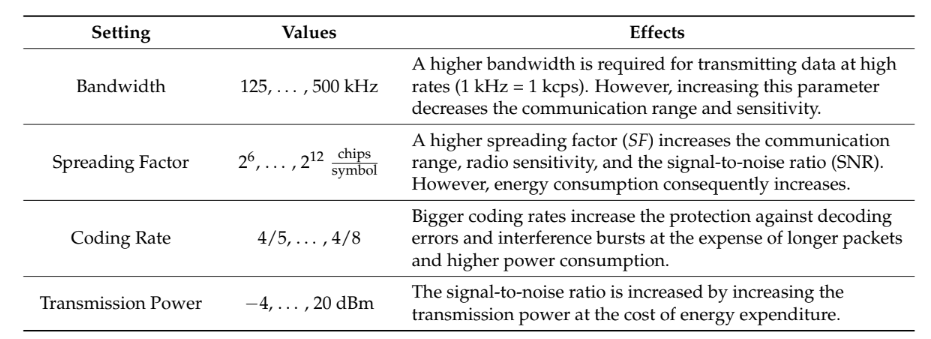
\includegraphics[width=\linewidth,keepaspectratio]{./imagenes/image79.png}

Opera en las bandas ISM de 433, 868 o 915 MHz, dependiendo de la región donde se implemente. Además, cada transmisión puede transportar una carga útil de entre 2 y 255 octetos \cite{ref30,ref31}.

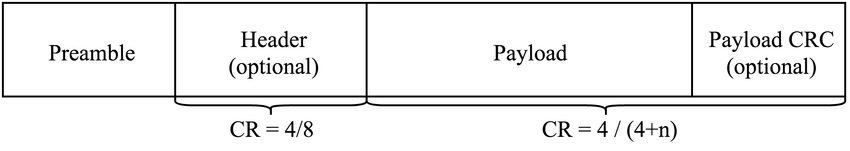
\includegraphics[width=\linewidth,keepaspectratio]{./imagenes/image66.png}

\subsubsection{Narrowband IoT}\label{narrowband-iot}

Es un estándar de comunicación inalámbrica diseñado para conectar dispositivos de bajo consumo a redes celulares usando una franja de banda muy angosta, apenas 180 kHz \cite{ref67}. Como menciona Antel, Nb-IoT es una evolución de LTE enfocados en la optimización de batería. Fue pensado específicamente para dispositivos que envían poca información (bajo ancho de banda) y con poca frecuencia \cite{ref68}.

NB-IoT tiene un link budget de 164 dB, mientras que GPRS y LTE tienen 144 dB y 142.7 dB respectivamente. Esto permite mucho mayor capacidad de penetración y alcance \cite{ref69}. Por otro lado, Antel tiene una cobertura de casi el 80\% del territorio uruguayo de NB-IoT \cite{ref68}.

\subsubsection{DVB-S2 (Europeo)}\label{dvb-s2-europeo}

DVB-S2 (\emph{Digital Video Broadcasting} - Segunda Generación) es un sistema flexible de modulación y codificación de canal diseñado para aplicaciones de banda ancha por satélite. Fue desarrollado como sucesor de los estándares DVB-S y DVB-DSNG originales, aprovechando los avances tecnológicos para ofrecer aproximadamente un 30\% más de capacidad bajo las mismas condiciones de ancho de banda y potencia del transpondedor \cite{ref27}.

El estándar incluye \cite{ref27}:

\begin{itemize}
\item
  Corrección de Errores (FEC): Utiliza un sistema potente basado en códigos LDPC (\emph{Low-Density Parity Check}) concatenados con códigos BCH. Esto permite que el sistema opere muy cerca del límite de Shannon.
\item
  Modulación Flexible: DVB-S2 soporta cuatro constelaciones: QPSK, 8PSK, 16APSK y 32APSK. Mientras que QPSK y 8PSK son ideales para aplicaciones limitadas por potencia, como la radiodifusión. 16APSK y 32APSK están optimizadas para servicios limitados por ancho de banda. A diferencia de QPSK y 8PSK, ofrecen una eficiencia espectral mucho mayor, pero son más sensibles a distorsiones no lineales.
\item
  Herramientas Avanzadas de Adaptación:

  \begin{itemize}
  \item
    ACM (\emph{Adaptive Coding and Modulation}): Optimiza dinámicamente la codificación y la modulación cuadro a cuadro para ajustarse a las condiciones actuales de propagación.
  \item
    VCM (\emph{Variable Coding and Modulation}): Permite diferentes niveles de protección contra errores para distintos componentes del servicio.
  \end{itemize}
\end{itemize}

\begin{itemize}
\item
  Eficiencia Espectral: Ofrece tres factores de \emph{roll-off} (0.35, 0.25 y 0.20) para moldear el espectro de la señal y optimizar el uso del ancho de banda.
\end{itemize}

DVB-S2 es compatible con servicios de televisión codificados MPEG-2 y MPEG-4 \cite{ref27}.

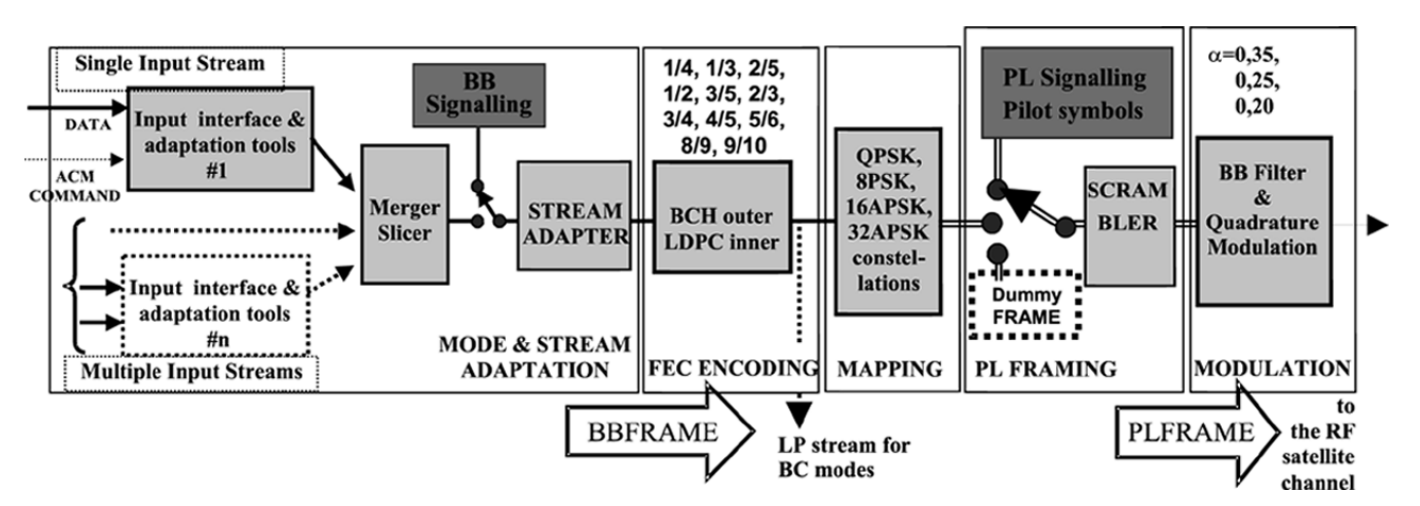
\includegraphics[width=\linewidth,keepaspectratio]{./imagenes/image15.png}

\subsubsection{Radios definidos por software}\label{radios-definidos-por-software}

Un SDR es un sistema de comunicación por radio donde los componentes que tradicionalmente se implementan en hardware (como filtros, amplificadores y moduladores) se definen mediante software \cite{ref49}.

\hl{A diferencia de los dispositivos de radio convencionales, que son estrictamente de hardware y tienen especificaciones fijas (como rangos de frecuencia y filtros predeterminados), un SDR ofrece una gran flexibilidad. Esto nos permite ajustar parámetros como la frecuencia, el ancho de banda y el método de modulación o demodulación utilizando programas informáticos sin necesidad de cambiar o comprar más componentes físicos.}

\subsubsection{Elección de banda}\label{elecciuxf3n-de-banda}

Los factores involucrados en la elección de banda son los siguientes:

\begin{enumerate}
\def\labelenumi{\arabic{enumi}.}
\item
  Pérdida de Trayectoria en Espacio Libre (FSPL): Teóricamente, la pérdida en el espacio libre es directamente proporcional al cuadrado de la frecuencia \cite{ref39}.

  \(L_{FS} = \ {(\frac{4\pi df}{c})}^{2}\)

  \(L_{FS}\) : pérdida por propagación

  \(d\) : \hl{velocidad de la luz}

  \(f\) : frecuencia

  \(c\) : velocidad de la luz

  A frecuencias más altas (como la banda Ka), las pérdidas son mucho mayores que en frecuencias bajas (como UHF), lo que requiere compensar con mayor potencia de transmisión o antenas de mayor ganancia \cite{ref39}.
\item
  Capacidad del Canal (Ecuación de Shannon): La necesidad de mayores tasas de datos (por ejemplo, para transmitir video) impulsa el uso de frecuencias más altas. Según la Ecuación de Shannon, la capacidad de información de un canal está ligada a su ancho de banda y a la relación señal-ruido \cite{ref39}.

  \(C\  = \ B\log_{2}(1\  + \ SNR)\)
\end{enumerate}

\(C\) : Capacidad

\(B\) : Ancho de banda

\(SNR\) : Relación señal a ruido

\begin{quote}
Las bandas superiores (X, Ka) ofrecen un ancho de banda mucho mayor, permitiendo tasas de transferencia de datos superiores a 100 Mbps, mientras que las bandas VHF/UHF suelen estar limitadas a tasas bajas para telemetría y comando \cite{ref39}.
\end{quote}

\begin{enumerate}
\def\labelenumi{\arabic{enumi}.}
\setcounter{enumi}{2}
\item
  Ganancia de la Antena y Apuntamiento: El área efectiva (o apertura efectiva) de una antena es una medida de su capacidad para extraer potencia de una onda electromagnética incidente. En términos sencillos, representa la superficie "útil" de la antena que realmente captura la señal \cite{ref39}.
\end{enumerate}

\(A_{ef} = \ \frac{G\lambda^{2}}{4\pi}\)

\(A_{ef}\) : Área efectiva de apertura

\(G\) : \hl{Ganancia}

\hl{}\(\lambda\) \hl{: Longitud de onda}

\begin{quote}
\hl{Para mantener una ganancia constante, si se aumenta la frecuencia (reduciendo la longitud de onda), el área efectiva necesaria disminuye drásticamente. El aumento de la ganancia mediante el incremento de la frecuencia o del área efectiva resulta en un ancho de haz más estrecho. Esto exige una precisión de apuntamiento mucho mayor hacia la estación terrestre para no perder el enlace} \cite{ref39}\hl{.}

\hl{En el caso de las antenas omnidireccionales, su área efectiva es inherentemente pequeña y depende principalmente del cuadrado de la longitud de onda, lo que las hace muy dependientes de la frecuencia para cerrar el enlace} \cite{ref39}\hl{}\cite{ref40}\hl{.}
\end{quote}

\begin{enumerate}
\def\labelenumi{\arabic{enumi}.}
\setcounter{enumi}{3}
\item
  \hl{Atenuación Atmosférica y Ruido: Las frecuencias superiores sufren una mayor atenuación por gases atmosféricos y lluvia debido a la interacción física entre las ondas electromagnéticas de longitud de onda corta y las moléculas presentes en la atmósfera} \cite{ref40}\hl{.}
\end{enumerate}

\subsection{Video digital}\label{video-digital}

\subsubsection{Codificación de video}\label{codificaciuxf3n-de-video}

La codificación de video es el proceso mediante el cual se comprime y se transforma el formato de un contenido de video sin procesar en un archivo digital, de modo que pueda reproducirse en distintos dispositivos y plataformas.

\textbf{Input}: Video Crudo Digital (formato YUV)

\textbf{Output}: Video Comprimido (formato H.264, H.265)

El objetivo principal de este proceso es reducir el tamaño del archivo. Para lograrlo, se eliminan datos que no son esenciales. Al reproducirse, el video resultante no es una copia exacta del original, sino una aproximación suficientemente fiel. En el caso del streaming en vivo, es especialmente importante, ya que al comprimir el video se disminuye el uso de ancho de banda, facilitando su transmisión desde la fuente hasta el reproductor, sin sacrificar la calidad percibida por los usuarios \cite{ref24}.

El códec H.264 (AVC) destaca por su buena eficiencia de compresión, permitiendo reducir significativamente el tamaño del video manteniendo una calidad aceptable, además de requerir un bajo costo computacional y ofrecer alta velocidad de codificación, lo que lo hace ideal para aplicaciones en tiempo real. Su principal limitación es que es menos eficiente que códecs más modernos, por lo que necesita mayores tasas de bits para lograr la misma calidad. A pesar de esto, sigue siendo ampliamente utilizado debido a su compatibilidad casi universal con dispositivos.

El códec H.265 (HEVC) presenta como principal ventaja su alta eficiencia de compresión, ya que permite obtener la misma calidad de video utilizando aproximadamente un 40--50\% menos de bitrate que H.264, lo que reduce significativamente el consumo de ancho de banda y el tamaño de los archivos. Sin embargo, requiere una mayor capacidad de procesamiento, lo que implica tiempos de codificación más largos y mayores exigencias de hardware.

\subsubsection{Encapsulamiento}\label{encapsulamiento}

La encapsulación es el proceso de envolver datos de video codificados en unidades estructuradas y paquetizadas para facilitar su transmisión, almacenamiento y sincronización en distintos sistemas multimedia. En el caso de los estándares HEVC (H.265) y AVC (H.264), ambos utilizan una capa de abstracción, llamada Network Abstraction Layer, para cumplir esta función \cite{ref26}.

\textbf{Input}: Video Comprimido (formato H.264, H.265)

\textbf{Output}: Paquetes Transport Stream

El MPEG-2 Transport Stream (TS) es un estándar global utilizado para la difusión de televisión digital (vía satélite, cable y terrestre), el almacenamiento en discos ópticos (como Blu-ray) y sistemas de IPTV gestionados. Su función principal es definir la multiplexación y sincronización de datos de audio y video comprimidos \cite{ref26}.

Los datos codificados (unidades NAL) se empaquetan primero en PES (Packetized Elementary Stream). El encabezado PES contiene información de temporización esencial, como una base de reloj común y marcas de tiempo para indicar cuándo se deben decodificar (DTS) y presentar (PTS) los datos. Los paquetes PES se fragmentan en unidades de longitud fija de 188 bytes. Esta estructura de longitud fija es fundamental para entornos donde es probable que ocurran errores, ya que facilita que el receptor mantenga la sincronización en canales con pérdidas. Cada paquete TS incluye un PID en su encabezado para identificar a qué componente (video, audio o datos) pertenece, permitiendo al receptor demultiplexar los servicios \cite{ref26}.

\subsection{Componentes de RF}\label{componentes-rf}

\subsubsection{Amplificador de potencia}\label{amplificador-de-potencia}

Un amplificador de potencia (PA) convierte señales de baja potencia en una de mayor potencia \cite{ref88}. Los parámetros clave que se toman en cuenta para seleccionar amplificadores son los siguientes:

\begin{itemize}
\item
  Ganancia: Mide cuánto aumenta la señal de entrada de un amplificador de potencia de RF, expresado en decibelios (dB) como la relación de salida a potencia de entrada \cite{ref89}.
\item
  Eficiencia: Refiere a la eficacia con la que la potencia de CC de entrada se convierte en potencia de salida de RF, expresada típicamente como un porcentaje. La alta eficiencia minimiza el desperdicio de energía, reduce la generación de calor y extiende la vida útil de la batería \cite{ref89}.
\item
  Linealidad (IPn): Si un amplificador se comporta linealmente, entonces la señal de salida cambiará proporcionalmente a la señal de entrada \cite{ref90}. La no linealidad tiene como producto armónicos e interferencia intermodulación. Los productos de orden par tienden a ser fáciles de filtrar. Los de orden impar son más difíciles de filtrar porque los términos caen mas cerca de la banda útil. Debido a esto, el parámetro IP3 es una medida fundamental al tomar en cuenta el producto de tercer orden. Es el impar más significativo a excepción del primer orden \cite{ref91}. 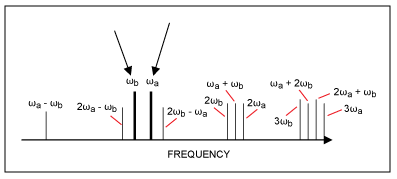
\includegraphics[width=3.0489in,keepaspectratio]{./imagenes/image18.png}
\item
  P1dB: Es el punto de compresión de un amplificador en el que su potencia de salida es 1 dB menor que la que tendría si mantuviera un comportamiento lineal ideal. Esta especificación permite determinar el límite superior de la región de operación lineal del amplificador. A partir de este punto, la ganancia comienza a disminuir y la potencia de salida deja de aumentar proporcionalmente con la potencia de entrada \cite{ref92}.
\end{itemize}

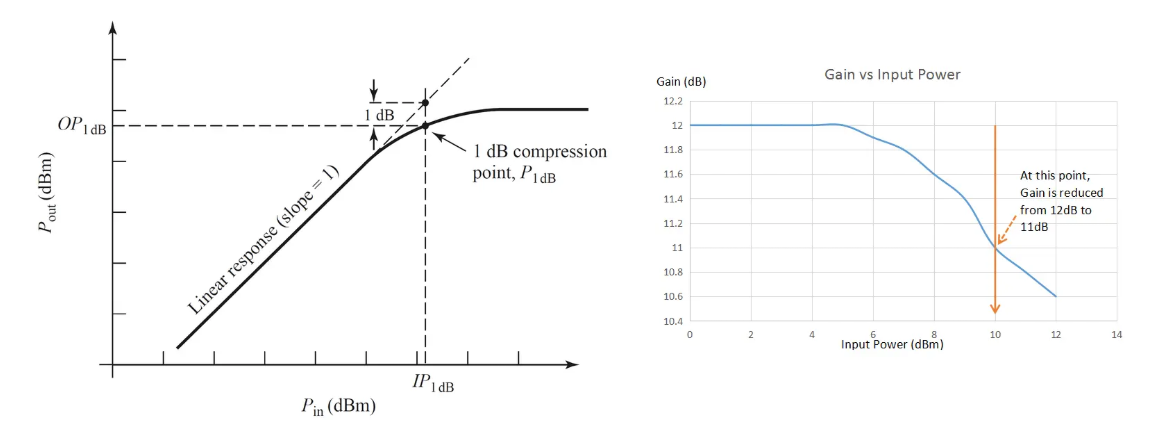
\includegraphics[width=\linewidth,keepaspectratio]{./imagenes/image62.png}

\cite{ref94}\begin{itemize}
\item
  Psat: Es la potencia máxima de salida de un amplificador. Corresponde al punto en el que el amplificador alcanza la saturación y ya no puede aumentar su potencia de salida, incluso si se continúa incrementando la potencia de entrada \cite{ref92}.
\item
  Frecuencia de operación: Define el espectro de frecuencias dentro del cual un amplificador de potencia de RF mantiene el rendimiento especificado \cite{ref93}.
\end{itemize}

\subsubsection{Amplificador de bajo ruido}\label{amplificador-de-bajo-ruido}

Un Amplificador de Bajo Ruido (LNA) es un componente electrónico fundamental ubicado en la etapa inicial de un receptor. Su función es amplificar las señales débiles captadas por la antena, incorporando la menor cantidad posible de ruido interno. Se utiliza principalmente para minimizar la temperatura de ruido total del sistema. Reduce de forma efectiva la contribución de ruido de todas las etapas posteriores de la cadena de recepción. Al amplificar la señal desde el comienzo y disminuir el efecto del ruido térmico generado por los componentes subsiguientes, el LNA permite mantener una relación señal-ruido (SNR) suficientemente alta para que el receptor pueda recuperar correctamente los datos transmitidos del ruido de fondo \cite{ref40}.

\subsubsection{Atenuadores}\label{atenuadores}

Un atenuador es un componente pasivo que introduce una pérdida conocida y fija (en dB) entre el transmisor y el receptor. La idea es reemplazar el espacio libre por un atenuador calibrado que simule la atenuación que tendría la señal a esa distancia real. Primero se calcula la atenuación que se quiere simular con la fórmula de espacio libre (FSPL), que depende de la distancia y la frecuencia. Los atenuadores comerciales vienen en valores fijos (3, 6, 10, 20, 30 dB) y soportan una potencia determinada que el transmisor no puede superar. Se combinan varios en cascada para sumar el valor objetivo. Se prueba transmitiendo paquetes reales y revisando RSSI/SNR en el receptor, aumentando la atenuación gradualmente hasta encontrar el punto donde empieza a fallar. Esto da el margen de enlace real, útil para anticipar pérdidas adicionales en vuelo.

\subsubsection{Construcción y materiales de antenas}\label{construcciuxf3n-y-materiales-antenas}

La velocidad de propagación de la onda de radio a lo largo de un hilo conductor de cobre es ligeramente menor que la velocidad de la luz en el espacio libre. Debido al propio material y otros efectos capacitivos, la longitud del elemento radiador suele ser aproximadamente 5\% menor que la longitud teórica de un cuarto de onda \cite{ref70}.

Materiales conductores para radiadores \cite{ref70}:

\begin{itemize}
\item
  Cobre: Es el estándar para antenas de hilo, como dipolos y sistemas de radiales, debido a su conductividad superior, que minimiza las pérdidas por resistencia y maximiza la eficiencia del sistema.
\item
  Aluminio: El aluminio es el material predilecto para estructuras rígidas como antenas Yagi, mástiles y radiadores verticales, debido a su excelente relación resistencia-peso y su bajo costo. Su utilización en forma de tubos de mayor diámetro que un cable convencional permite que las antenas operen con un mayor ancho de banda. Además, el aluminio es fácil de mecanizar manualmente y no se oxida fácilmente.
\end{itemize}

\subsection{Interfaces de comunicación}\label{interfaces-comunicacion}

\subsubsection{SPI}\label{spi}

SPI (Serial Peripheral Interface) es un protocolo de comunicación digital utilizado para conectar un microcontrolador con sensores, memorias, pantallas y otros periféricos.

\begin{itemize}
\item
  Serial: Los bits se envían uno detrás de otro.
\item
  Peripheral: Permite la comunicación entre un dispositivo principal y periféricos.
\item
  Interface: Define la forma en que se conectan y comunican los componentes.
\end{itemize}

\textbf{Características}

\begin{itemize}
\item
  Síncrono: utiliza una señal de reloj para sincronizar la comunicación.
\item
  Full Duplex: permite enviar y recibir datos al mismo tiempo.
\item
  Main - Subnode: existe un dispositivo principal (Main) y uno o varios dispositivos subordinados (Subnodes). También conocido como Master-Slave.
\end{itemize}

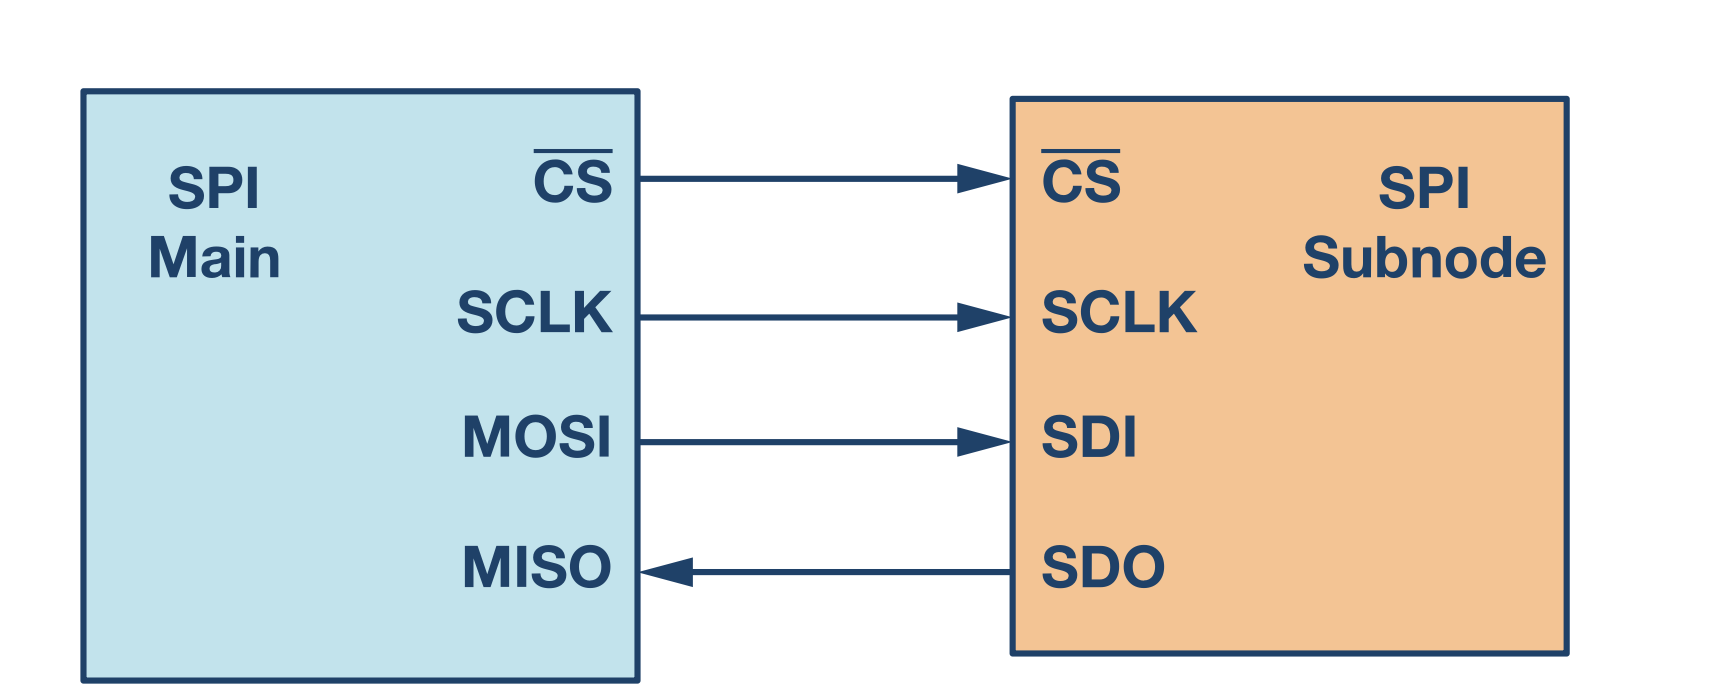
\includegraphics[width=3.2135in,keepaspectratio]{./imagenes/image68.png}

\textbf{Lineas}

\begin{enumerate}
\def\labelenumi{\arabic{enumi}.}
\item
  SCLK (Serial Clock): Es la señal de reloj generada por el Main. Esta señal sincroniza la transmisión y recepción de datos entre el Main y el Subnode. Se le llama Serial Clock porque sincroniza la transmisión serial de los datos, es decir, bit a bit.
\item
  CS (Chip Select): Es la señal utilizada por el Main para seleccionar con qué Subnode desea comunicarse. Normalmente esta señal permanece en 1. Cuando el Main quiere comunicarse con un Subnode específico, coloca su línea CS en nivel 0. Cada Subnode posee una línea CS independiente.
\item
  Líneas de Datos: SPI utiliza dos líneas de datos independientes, lo que permite la comunicación Full Duplex.

  \begin{enumerate}
  \def\labelenumii{\alph{enumii}.}
  \item
    MOSI (Main Out, Subnode In): Línea utilizada para transmitir datos desde el Main hacia el Subnode.
  \item
    MISO (Main In, Subnode Out): Línea utilizada para transmitir datos desde el Subnode hacia el Main.
  \end{enumerate}
\end{enumerate}

\cite{ref80}\textbf{Funcionamiento}

\begin{enumerate}
\def\labelenumi{\arabic{enumi}.}
\item
  Shifting: Consiste en desplazar los bits dentro de un registro para transmitir el siguiente bit por la línea de comunicación. (Cambiar el bit a enviar)
\item
  Sampling Consiste en leer o capturar el valor presente en la línea de datos en un instante determinado por el reloj.
\end{enumerate}

\cite{ref80}\textbf{Secuencia de comunicación}

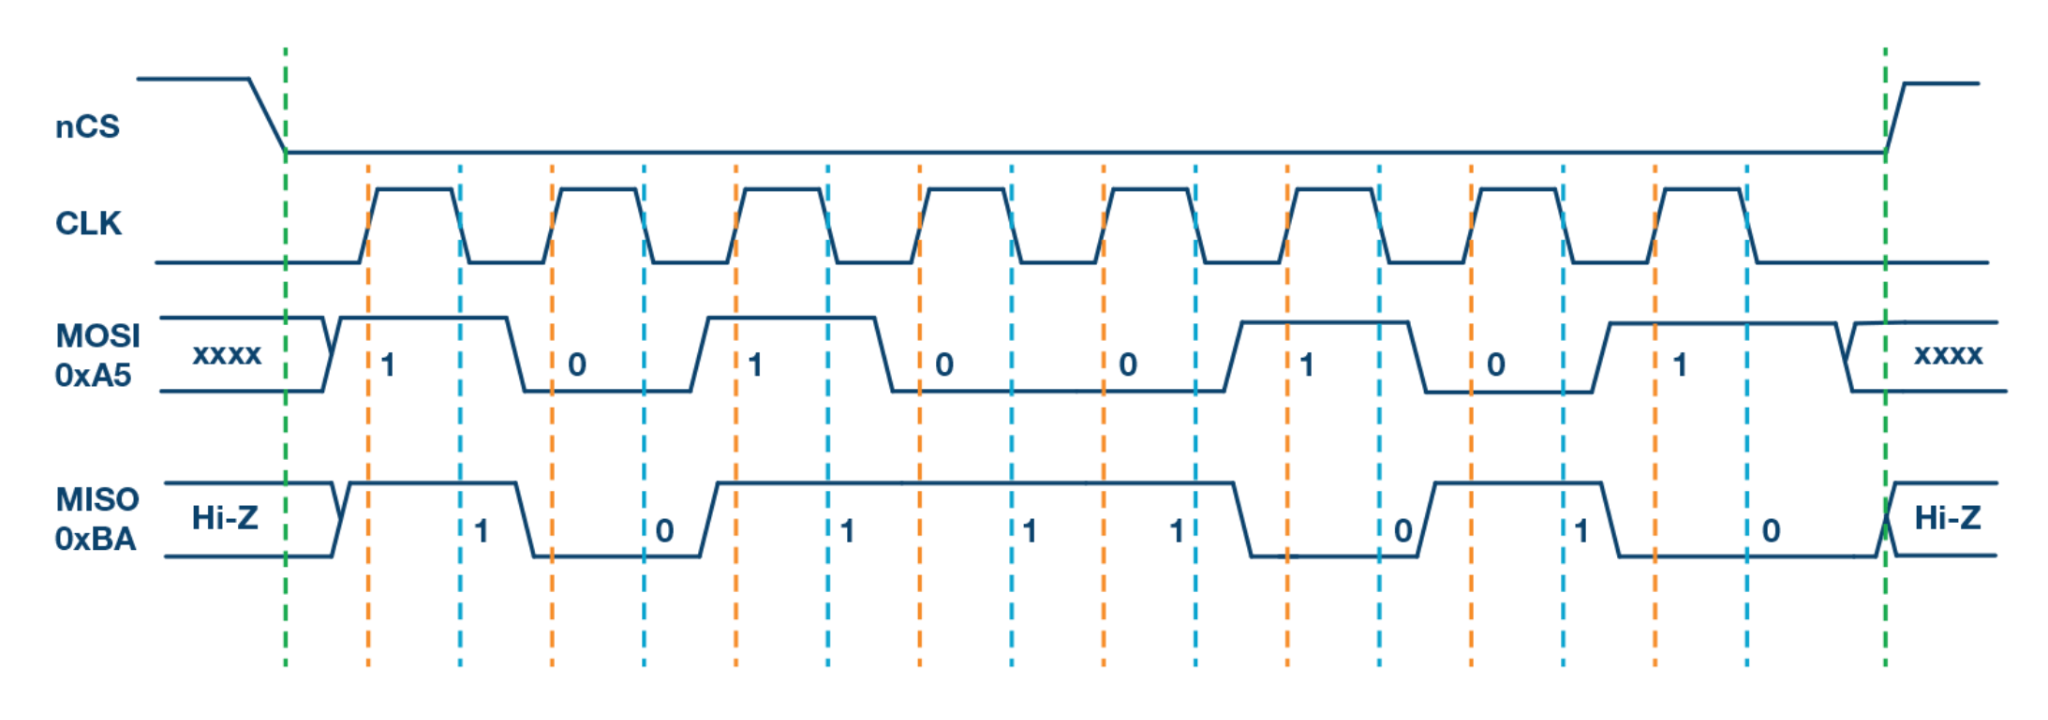
\includegraphics[width=\linewidth,keepaspectratio]{./imagenes/image53.png}

\begin{enumerate}
\def\labelenumi{\arabic{enumi}.}
\item
  El Main coloca la señal CS pasa a 0, seleccionando el Subnode.
\item
  El Main comienza a generar la señal de reloj (SCLK).
\item
  MOSI (Main → Subnode): En cada flanco de subida del reloj (línea naranja), el Subnode lee (samplea) el bit enviado por el Main. En cada flanco de bajada (línea azul), el Main actualiza la línea MOSI con el siguiente bit a transmitir (shift).
\item
  MISO (Subnode → Main): En cada flanco de subida del reloj (línea naranja), el Main lee (samplea) el bit enviado por el Subnode. En cada flanco de bajada (línea azul), el Subnode actualiza la línea MISO con el siguiente bit a transmitir (shift).
\end{enumerate}

\cite{ref80} La configuración de si se lee en la subida o bajada del clock depende de los parámetros CPOL (Clock Polarity) y CPHA (Clock Phase) que tanto el Main como el Subnode deben configurarse previamente con el mismo modo SPI para que la comunicación funcione. Hay 4 modos diferentes \cite{ref80}.

\textbf{Múltiples subnodos SPI}

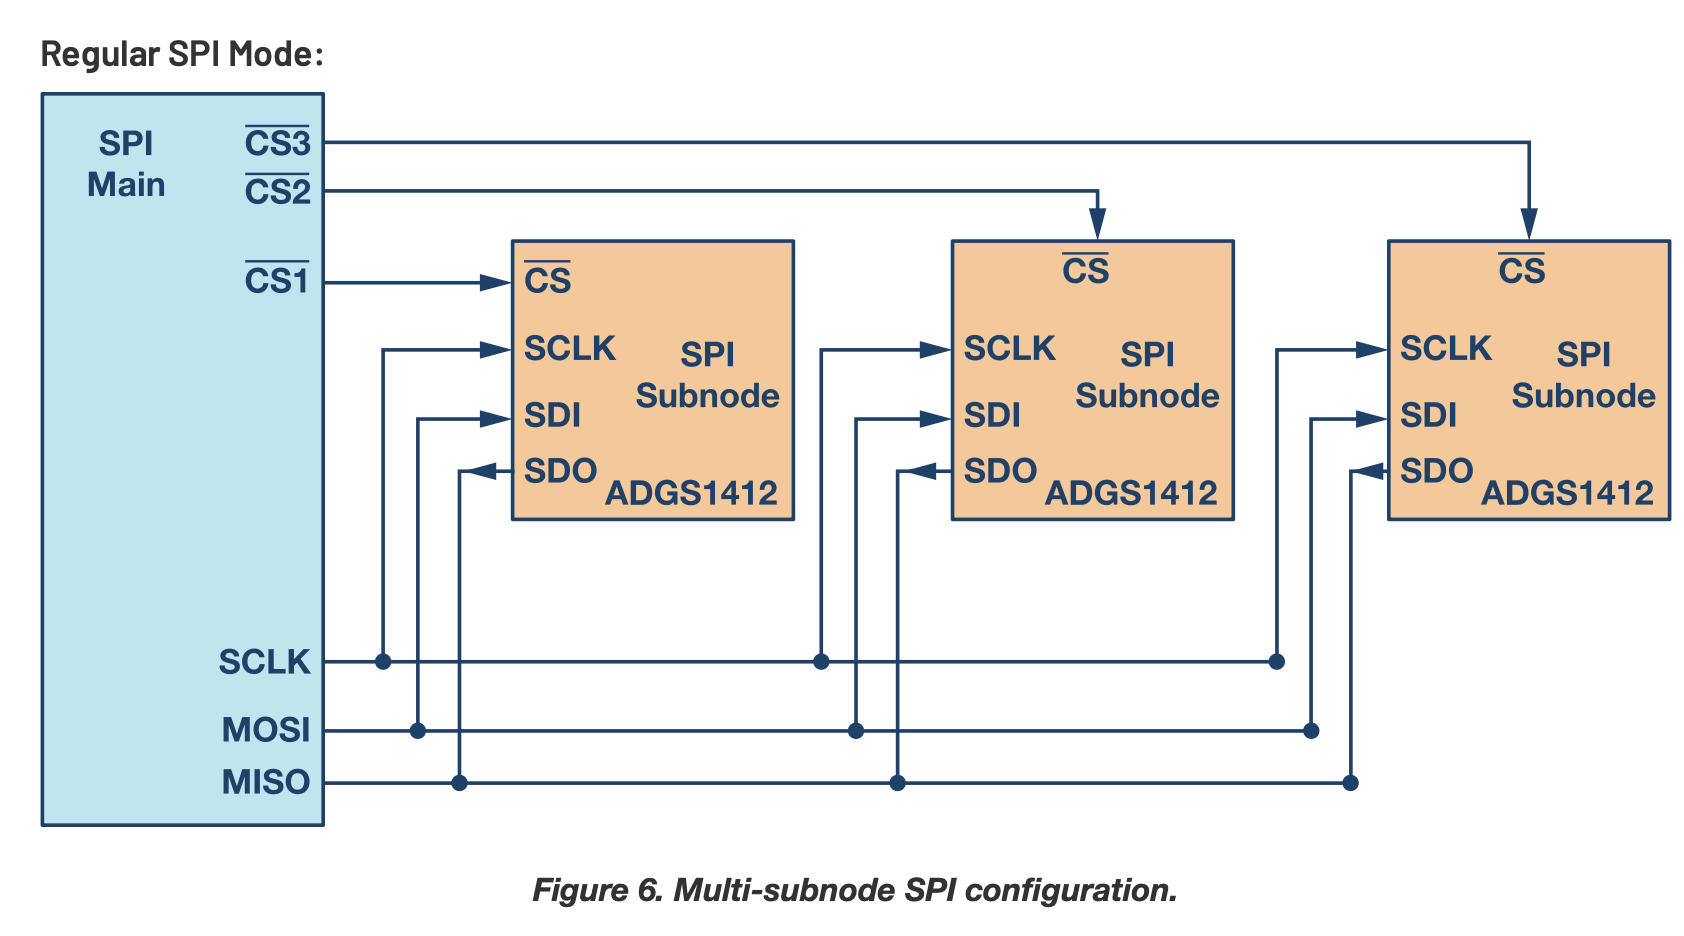
\includegraphics[width=\linewidth,keepaspectratio]{./imagenes/image46.png}

Todos los dispositivos comparten:

\begin{enumerate}
\def\labelenumi{\arabic{enumi}.}
\item
  MOSI
\item
  MISO
\item
  SCLK
\end{enumerate}

Sin embargo, cada dispositivo posee una línea CS independiente. El Main selecciona el dispositivo con el que desea comunicarse colocando su señal CS correspondiente en 0, mientras mantiene las demás en 1 \cite{ref80}.

\subsubsection{I2C}\label{i2c}

I2C (Inter-Integrated Circuit) es un protocolo de comunicación digital utilizado para conectar un microcontrolador con sensores, memorias, pantallas y otros periféricos utilizando únicamente dos líneas principales.

\textbf{Características}

\begin{itemize}
\item
  Síncrono: utiliza una señal de reloj para sincronizar la comunicación.
\item
  Half Duplex: no transmite y recibe datos al mismo tiempo por líneas separadas, sino que ambos sentidos usan la misma línea SDA.
\item
  Multi-main y multi-node: puede haber uno o varios dispositivos principales y varios sub nodos conectados al mismo bus.
\item
  Direccional por dirección: cada subnodo tiene una dirección propia de 7 bits o 10 bits.
\end{itemize}

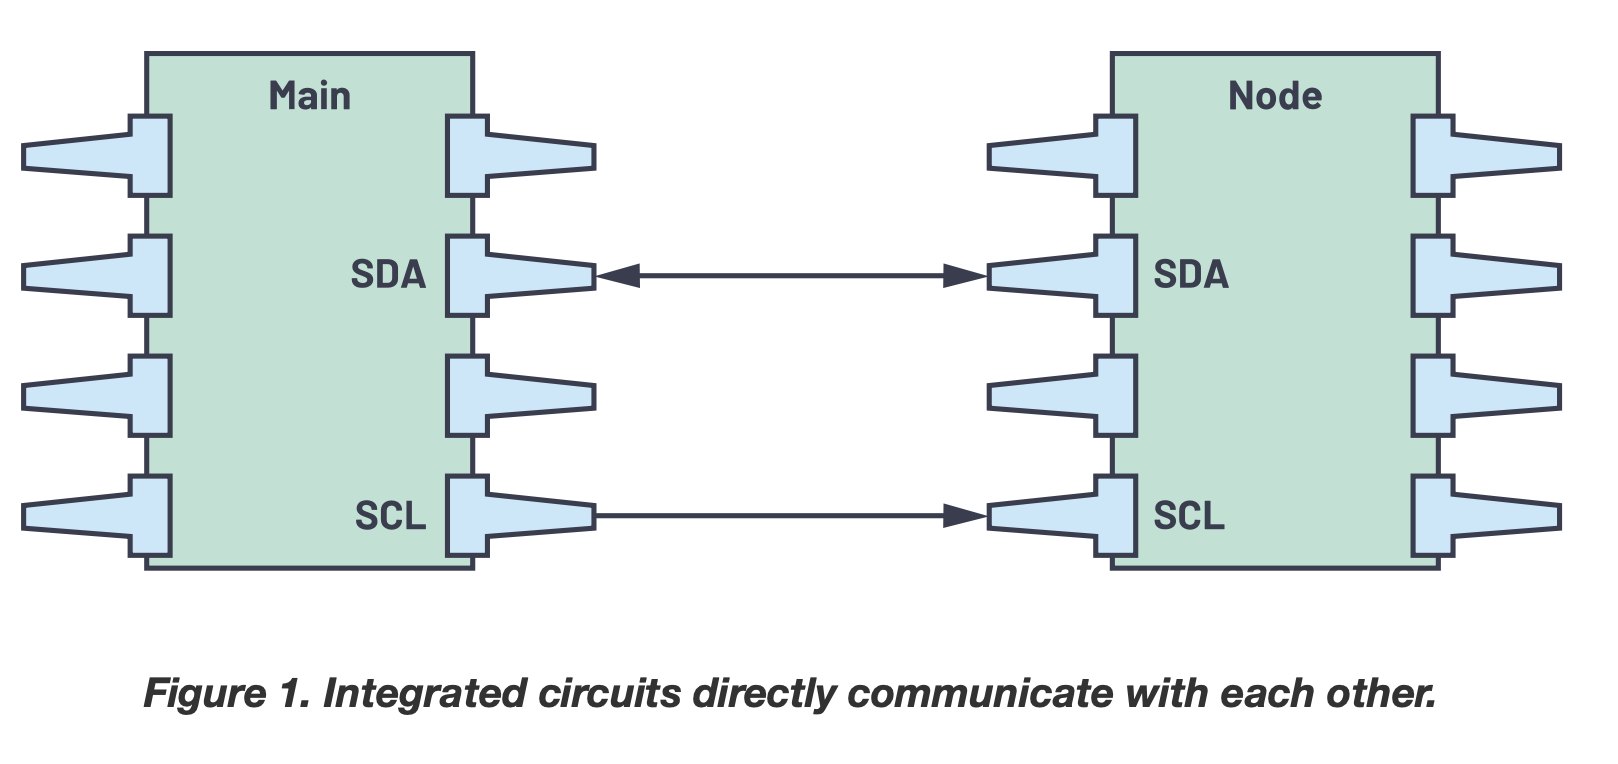
\includegraphics[width=\linewidth,keepaspectratio]{./imagenes/image27.png}

\textbf{Lineas}

\begin{itemize}
\item
  SDA (Serial Data): línea bidireccional usada para enviar y recibir datos.
\item
  SCL (Serial Clock): línea de reloj generada normalmente por el Main. Sirve para sincronizar cuándo se leen los bits.
\end{itemize}

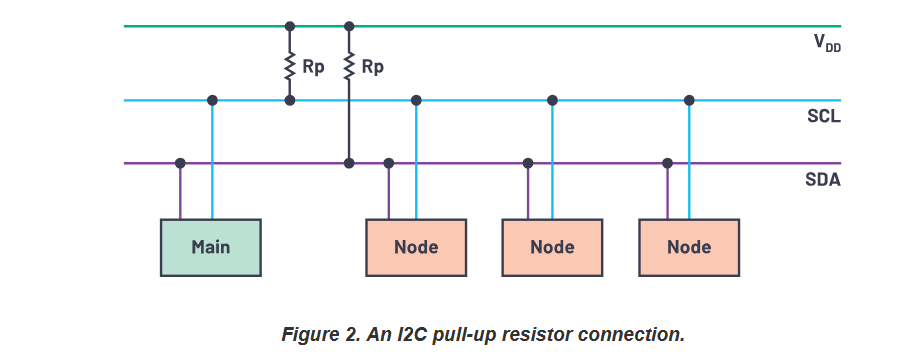
\includegraphics[width=\linewidth,keepaspectratio]{./imagenes/image76.png}

\textbf{Resistencias Pull-Up}

En I2C, las líneas SDA y SCL usan resistencias de pull-up (Rp). Estas resistencias hacen que las líneas estén por defecto en HIGH.

\begin{itemize}
\item
  Para enviar un 0, el dispositivo baja la línea a LOW.
\item
  Para enviar un 1, el dispositivo libera la línea y la resistencia la vuelve a subir a HIGH.
\end{itemize}

Esto permite que varios dispositivos compartan el mismo bus sin que uno fuerce HIGH mientras otro fuerza LOW.

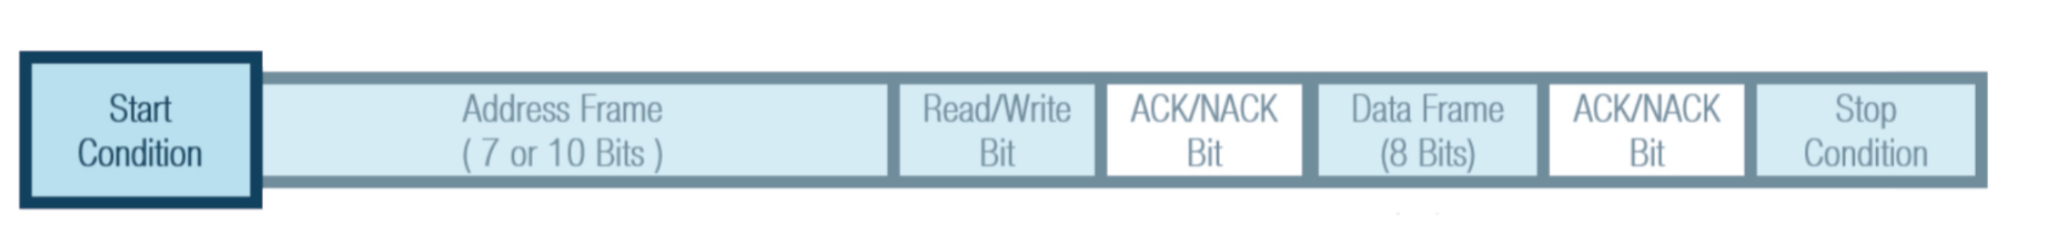
\includegraphics[width=\linewidth,keepaspectratio]{./imagenes/image32.png}

\cite{ref81}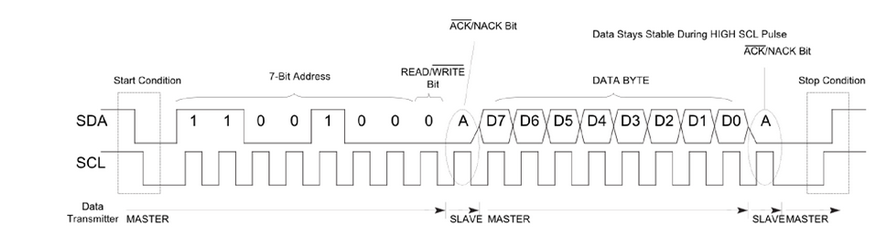
\includegraphics[width=\linewidth,keepaspectratio]{./imagenes/image86.png}

\cite{ref82}\textbf{Proceso de Transmisión \cite{ref81}}

\begin{enumerate}
\def\labelenumi{\arabic{enumi}.}
\item
  El Main genera una condición de START, bajando SDA de HIGH a LOW mientras SCL está en HIGH. (La señal de clock estaba ``apagada'' y ahora arranca)
\item
  El Main envía la dirección del subnodo con el que quiere comunicarse.
\item
  También envía un bit que indica si quiere escribir o leer.
\item
  El subnodo que reconoce su dirección responde con un ACK, bajando SDA.
\item
  Se transmite el frame de datos.
\item
  Después de cada dato recibido, el receptor correspondiente envía otro ACK.
\item
  Para terminar, el Main genera una condición de STOP, subiendo SDA a HIGH mientras SCL está en HIGH.
\end{enumerate}

\textbf{Múltiples subnodos I2C}

Todos los dispositivos comparten \cite{ref81}:

\begin{itemize}
\item
  SDA
\item
  SCL
\end{itemize}

A diferencia de SPI, no hace falta una línea CS para cada dispositivo. El Main selecciona con quién comunicarse enviando la dirección del subnodo.

\subsubsection{UART}\label{uart}

UART (Universal Asynchronous Receiver-Transmitter) es un protocolo de comunicación serie asíncrono que utiliza dos líneas principales: Transmitter (Tx) y Receiver (Rx). Al ser asíncrono, no existe una señal de reloj compartida entre los dispositivos.

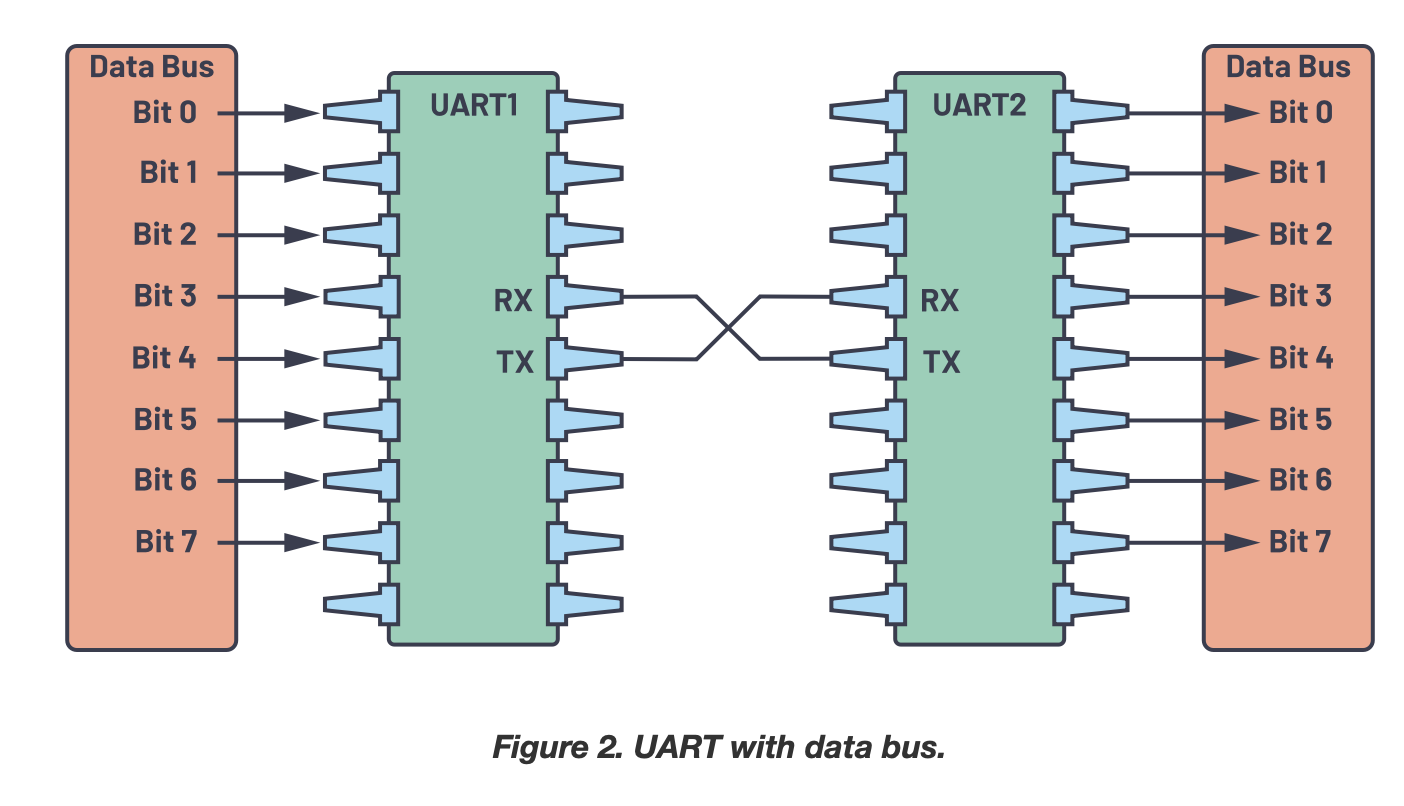
\includegraphics[width=\linewidth,keepaspectratio]{./imagenes/image19.png}

\cite{ref83} El Databus quiere enviar los bits en paralelo y la interfaz UART se encarga de transmitirlos de forma serial (uno atrás del otro). Este protocolo es entre dos dispositivos y no más. El TX de uno está conectado al RX del otro \cite{ref83}.

Para que la comunicación funcione correctamente, ambos dispositivos deben configurarse previamente con el mismo baud rate. El baud rate indica la velocidad a la que se transmiten los bits por segundo. Cada dispositivo utiliza su propio reloj interno para enviar y muestrear los datos, por lo que la clave es que ambos tengan configuraciones compatibles para minimizar errores \cite{ref83}.

La línea UART permanece en estado HIGH por defecto. Cuando el transmisor desea enviar información, lleva la línea a LOW durante un tiempo de bit, generando el bit de arranque (Start Bit). Este cambio de HIGH a LOW le indica al receptor que comienza una nueva trama de datos \cite{ref83}.

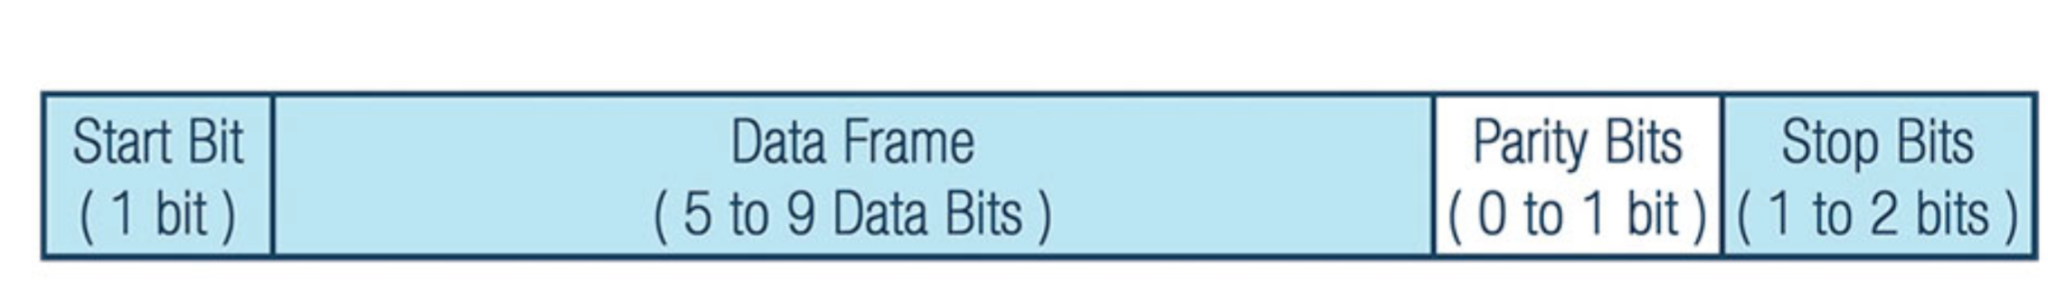
\includegraphics[width=\linewidth,keepaspectratio]{./imagenes/image57.png}

\cite{ref83} La estructura de una trama UART se divide de la siguiente manera \cite{ref83}:

\begin{enumerate}
\def\labelenumi{\arabic{enumi}.}
\item
  \textbf{Bit de arranque}

  \begin{itemize}
  \item
    Se mantiene siempre en nivel 0 (LOW).
  \item
    Su función es notificar al receptor el inicio de una nueva transmisión de datos.
  \end{itemize}
\item
  \textbf{Bits de datos}

  \begin{itemize}
  \item
    Representan la información útil o carga útil (payload) a transmitir.
  \item
    Dependiendo de la configuración previa, suelen ser 5, 6, 7, 8 o hasta 9 bits.
  \item
    Por lo general, el envío se realiza comenzando por el bit menos significativo (LSB).
  \end{itemize}
\item
  \textbf{Bit de paridad}

  \begin{itemize}
  \item
    Permite implementar un mecanismo básico para la detección de errores simples.
  \item
    Las opciones incluyen paridad par (Even), impar (Odd) o puede omitirse según se requiera.
  \end{itemize}
\item
  \textbf{Bit(s) de parada}

  \begin{itemize}
  \item
    Puede consistir en uno, uno y medio o dos bits de duración.
  \item
    Estos bits permanecen siempre en estado 1 (HIGH).
  \item
    Señalan la conclusión de la trama actual, permitiendo que el receptor se sincronice para la próxima ráfaga.
  \end{itemize}
\end{enumerate}

\textbf{Proceso de Transmisión} \cite{ref83}\begin{enumerate}
\def\labelenumi{\arabic{enumi}.}
\item
  Los datos suelen existir inicialmente en paralelo dentro del dispositivo.
\item
  La interfaz UART transmisora convierte esos bits paralelos a una tira de bits serial (uno atrás del otro).
\item
  Luego coloca el Start Bit (LOW), transmite los bits de datos uno tras otro, opcionalmente agrega un bit de paridad para detección de errores y finalmente envía uno o más bits de parada (Stop Bits) en estado HIGH.
\item
  Durante la recepción, la UART receptora detecta el Start Bit y, utilizando su propio reloj interno, comienza a muestrear la línea para reconstruir los bits transmitidos.
\item
  Una vez recibidos todos los bits de la trama, convierte nuevamente la información de serie a paralelo y la entrega al sistema receptor.
\end{enumerate}

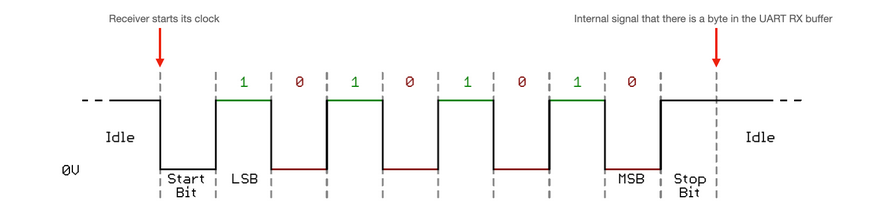
\includegraphics[width=\linewidth,keepaspectratio]{./imagenes/image14.png}

\cite{ref84} En UART no se puede mandar una cantidad variable de bits de datos dentro de una misma configuración. La cantidad de bits de datos, la presencia o no de bit de paridad, la cantidad de bits de parada y el baud rate deben configurarse previamente en ambos extremos. Como no existe una señal de reloj ni información adicional que indique dónde terminan los datos y dónde comienzan los bits de paridad o parada, el receptor necesita conocer de antemano el formato exacto de cada trama \cite{ref83}.

\subsection{Energía: baterías y conversores}\label{energia-fundamentos}

\subsubsection{Baterías}\label{baterias}

La energía solar no siempre está disponible durante las operaciones de una nave espacial. Para almacenar energía se utilizan baterías primarias y secundarias, las cuales se clasifican según su diferente composición electroquímica. Debido a que las baterías de tipo primario no son recargables, generalmente se utilizan en misiones de corta duración. Las baterías de plata-zinc (Ag-Zn) son utilizadas habitualmente debido a que son más fáciles de manipular y pueden descargarse a una mayor tasa. Sin embargo, también existe una variedad de baterías primarias basadas en litio que presentan una mayor densidad energética, entre ellas las de dióxido de azufre-litio (LiSO₂), monofluoruro de carbono-litio (LiCF\textsubscript{x}) y cloruro de tionilo-litio (LiSOCl₂) \cite{ref39}.

Las baterías de tipo secundario incluyen las de níquel-cadmio (NiCd), níquel-hidrógeno (NiH₂), polímero de litio (LiPo) e ion-litio (Li-ion), las cuales han sido ampliamente utilizadas en el pasado en pequeños satélites. Las baterías secundarias basadas en litio son utilizadas habitualmente en dispositivos electrónicos portátiles debido a su capacidad de recarga, bajo peso y alta densidad energética, y se han vuelto ampliamente utilizadas en misiones espaciales. Generalmente, se conectan a una fuente de energía primaria (por ejemplo, un panel solar) y pueden proporcionar energía recargable bajo demanda \cite{ref39}.

En general, existen dos grupos de celdas: de alta energía y de alta potencia. Las celdas de alta potencia utilizan un diseño de baja resistencia, por ejemplo, mediante el aumento del área superficial del recubrimiento o mediante múltiples puntos de contacto entre el colector de corriente y la celda. Esto permite reducir la resistencia total y alcanzar una mayor tasa de descarga. Por otro lado, las celdas de alta energía buscan optimizar la densidad energética gravimétrica para obtener la mayor cantidad de energía posible de la celda. En general, para aplicaciones espaciales es importante contar con una alta densidad energética, ya que una batería con una elevada densidad energética gravimétrica permite reducir el costo de lanzamiento a órbita al proporcionar una mayor capacidad de almacenamiento por unidad de masa \cite{ref39}.

Las baterías típicas de Li-ion presentan un rango de temperatura de operación de -20 °C a 60 °C. Esto puede no cumplir con los requisitos de misiones que requieren operar a temperaturas más bajas. Entre las baterías destinadas a aplicaciones de baja temperatura se encuentran \cite{ref39}:

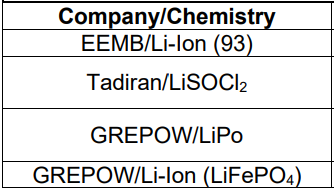
\includegraphics[width=2.1875in,keepaspectratio]{./imagenes/image33_1.png}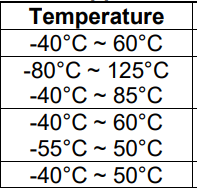
\includegraphics[width=1.2917in,keepaspectratio]{./imagenes/image33_2.png}\cite{ref39} En proyectos anteriores, \cite{ref2,ref3,ref99} se prefirieron las baterías de ion-litio. El equipo del proyecto Zephyrus X utilizó baterías de ion-litio 18650 como fuente de energía principal debido a su bajo peso, alta capacidad de potencia, posibilidad de recarga y amplio rango de temperatura de operación. Sin embargo, experiencias anteriores indicaron que el uso de baterías recargables no era la mejor opción. Si la batería se descargaba excesivamente, no podía volver a cargarse y, en algunos casos, llegaba a explotar {[}citar experiencia John{]}.

\subsubsection{Conversor de voltaje}\label{conversor-de-voltaje}

Dos tipos de conversores \cite{ref105}:

\begin{itemize}
\item
  Un conversor reductor disminuye el voltaje. Utiliza un interruptor electrónico que conecta y desconecta rápidamente la tensión de entrada. Un inductor y un capacitor suavizan esta señal para obtener una salida estable de menor voltaje. El voltaje de salida es una fracción del voltaje de entrada, determinada por el tiempo durante el cual el interruptor permanece encendido, conocido como ciclo de trabajo.
\item
  Un conversor elevador aumenta el voltaje. Utiliza un inductor para almacenar energía proveniente de la fuente de entrada. Cuando el interruptor se apaga, el inductor libera la energía almacenada. Esta energía se suma al voltaje de entrada, generando un voltaje de salida superior al de entrada.
\end{itemize}

Un conversor reductor es conocido por su excelente eficiencia en la conversión de potencia.

Es capaz de alcanzar de forma consistente eficiencias superiores al 95 \%. Esta elevada eficiencia implica que se desperdicia menos energía, lo que resulta fundamental para prolongar la duración de las baterías y reducir la generación de calor en dispositivos compactos \cite{ref105}.

Un conversor elevador también presenta una alta eficiencia, con valores que comúnmente superan el 90 \%. Un circuito bien diseñado puede alcanzar eficiencias máximas superiores al 95 \%. Sin embargo, generalmente opera en un rango de 85 \% a 95 \%. El proceso de aumentar el voltaje es ligeramente más complejo, lo que puede provocar mayores pérdidas de energía en comparación con un conversor reductor \cite{ref105}.

\subsection{Materiales y control térmico}\label{materiales-termico}

\subsubsection{Aluminio}\label{aluminio}

La conductividad térmica representa la capacidad de un material para transmitir calor. Se define como la cantidad de energía térmica que atraviesa una unidad de espesor del material, por unidad de área y por cada unidad de diferencia de temperatura. La elevada conductividad térmica del aluminio puro se debe principalmente al movimiento eficaz de los electrones libres \cite{ref85}.

La capacidad calorífica específica es una propiedad física que indica la cantidad de energía térmica requerida para aumentar en un grado Celsius (o un Kelvin) la temperatura de una unidad de masa de una sustancia. Esta propiedad es fundamental para la gestión térmica de los materiales, ya que determina la velocidad con la que estos absorben o liberan calor durante su operación. El aluminio puro destaca por su capacidad calorífica específica relativamente alta, que es de aproximadamente 0,900 kJ/(kg.K) a temperatura ambiente \cite{ref85} es decir, requiere una gran cantidad de energía térmica (calor) para elevar su temperatura en un grado Kelvin o Celsius.

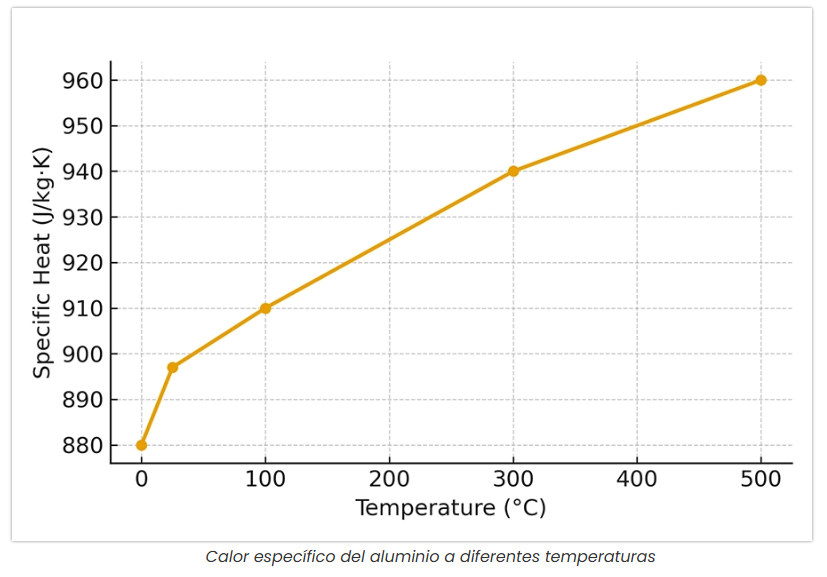
\includegraphics[width=3.3071in,keepaspectratio]{./imagenes/image90.png}

\cite{ref86} Si bien el aluminio es ampliamente reconocido por su alta capacidad para conducir el calor, también puede actuar como un excelente aislante frente a la radiación térmica gracias a su elevada reflectividad. En particular, es capaz de reflejar entre el 90 \% y el 95 \% de la radiación infrarroja incidente, reduciendo considerablemente la cantidad de energía térmica absorbida por el material \cite{ref85}.

Comparación de la conductividad térmica entre el cobre y el aluminio: El cobre y el aluminio son materiales ampliamente utilizados en aplicaciones de transferencia de calor, como radiadores e intercambiadores térmicos. Aunque el cobre presenta una conductividad térmica superior, el aluminio suele ser la opción preferida debido a su menor costo, menor densidad y mayor facilidad de fabricación y mecanizado \cite{ref85}.

\subsubsection{EPS}\label{eps}

El EPS tiene una conductividad térmica muy baja. Esto se debe a su estructura de celda cerrada, compuesta en un 98 \% de aire. Este aire atrapado dentro de las celdas es un conductor de calor muy deficiente, lo que le confiere a la espuma excelentes propiedades de aislamiento térmico \cite{ref87}.

\subsubsection{Control térmico}\label{control-termico}

El control térmico de una nave espacial tiene como objetivo principal mantener todos sus componentes dentro de los rangos de temperatura permitidos para sus requisitos operativos y de supervivencia en todas las fases de la misión. El comportamiento térmico de un satélite se rige por un balance de energía fundamentado en la cantidad de calor absorbido, almacenado, generado y disipado \cite{ref39}.

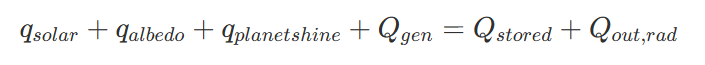
\includegraphics[width=\linewidth,keepaspectratio]{./imagenes/image82.png}

Los fundamentos de cada término son los siguientes \cite{ref39}:

\begin{itemize}
\item
  Fuentes de calor externas: Incluyen el calentamiento solar directo (q solar), el calentamiento solar reflejado por el planeta (q albedo) y el calentamiento por radiación infrarroja proveniente del planeta (q planetshine).
\item
  Generación de calor interna (Q gen): Depende de la disipación de energía de los componentes electrónicos y de carga útil de la nave espacial.
\item
  Almacenamiento de calor (Q stored): Se basa en la capacitancia térmica o masa térmica de la nave espacial.
\item
  Rechazo de calor (Q out,rad): En el vacío del espacio, el calor sólo puede disiparse mediante radiación infrarroja ya que no hay aire ni fluidos que permitan la transferencia de calor por convección.
\end{itemize}

\parte{Parte III: Diseño general del sistema}

\section{Requerimientos y arquitectura}\label{requerimientos-arquitectura}

\pendiente{Requerimientos y arquitectura.}

\subsection{Requerimientos del sistema}\label{requerimientos-sistema}

\pendiente{Requerimientos del sistema.}

\subsection{Arquitectura general: segmento de vuelo y segmento terrestre}\label{arquitectura-general}

\pendiente{Arquitectura general: segmento de vuelo y segmento terrestre.}

\subsection{Fases de la misión}\label{fases-mision}

\pendiente{Fases de la misión.}

\section{Diseño del enlace}\label{transmisiuxf3n}

ESCRIBIR UNA INTRO

\subsection{Distancia}\label{distancia}

Para definir la distancia máxima de transmisión, se investigaron proyectos de globos satélites lanzados en uruguay \cite{ref36}:

\begin{itemize}
\item
  GloboSat 01: Partió de la Base Aérea de Santa Bernardina, Durazno, y alcanzó una altura máxima de 34 km. Recuperaron la cápsula en las proximidades de la Quebrada de los Cuervos (Departamento de Treinta y Tres), habiendo recorrido aproximadamente 200 Km. Con una duración de vuelo de aproximadamente 3 horas y 15 minutos.
\item
  GloboSat 02: Partió de la Base Aérea de Santa Bernardina, Durazno, y alcanzó una altura máxima de 33,1 km. Aterrizó en Molles de Godoy (Lavalleja) habiendo recorrido una distancia horizontal de 130 km. El vuelo duró aproximadamente 2 horas y 55 minutos.
\end{itemize}

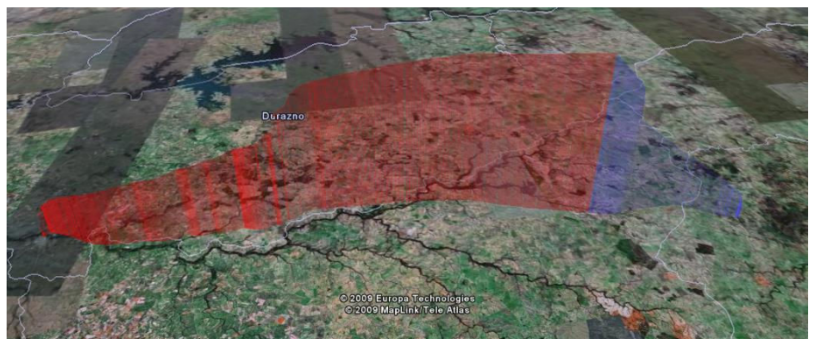
\includegraphics[width=3.7830in,keepaspectratio]{./imagenes/image85.png}

\cite{ref36} Recorrido vuelo GloboSat 02

\begin{itemize}
\item
  GloboSat 03: La distancia en línea recta desde el punto de lanzamiento hasta el aterrizaje fue de 40 km. Alcanzó una altura de 31.1 km y el vuelo duró 2 horas y 20 minutos.
\end{itemize}

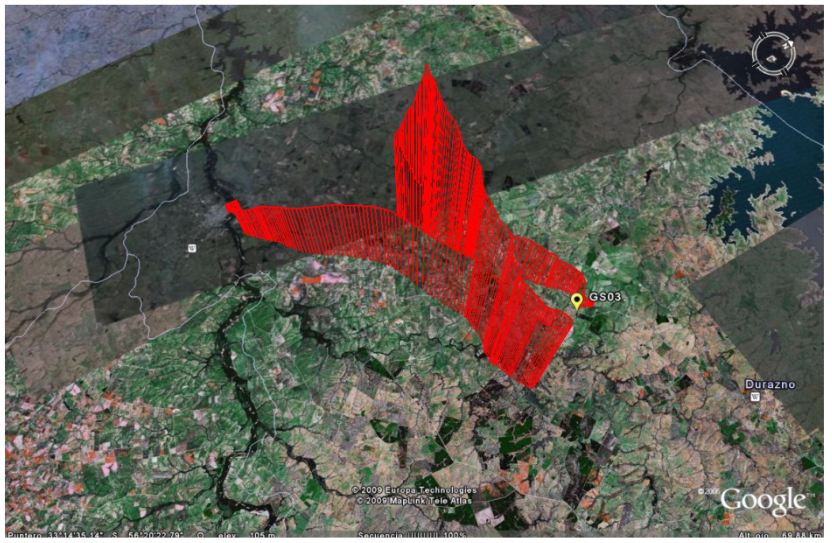
\includegraphics[width=3.0875in,keepaspectratio]{./imagenes/image49.png}

\cite{ref36} Recorrido vuelo GloboSat 03

Para la distancia del enlace de comunicación se tomó en cuenta el peor de los casos. Se realizó una predicción de la trayectoria utilizando la herramienta de Strato Flights \cite{ref37}. La herramienta utiliza las condiciones climáticas y del viento de la fecha ingresada para la predicción. Es evidente que no es exacto. En base a los lanzamientos de GloboSat, puede pasar cualquier cosa, porque depende de factores ambientales que no son predecibles. También depende de factores controlables como la velocidad de ascenso y descenso. Sin embargo, la predicción es útil para tomar como referencia el peor caso.

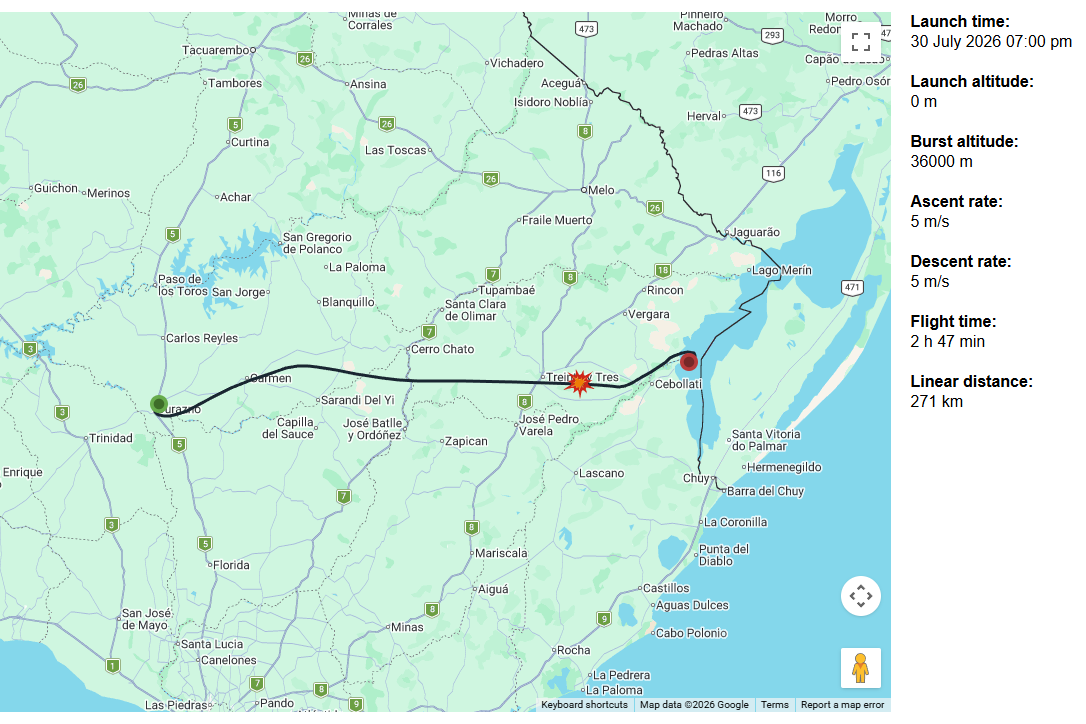
\includegraphics[width=\linewidth,keepaspectratio]{./imagenes/image84.png}

Utilizando la herramienta de SondeHub Predictor \cite{ref38} con los mismo parámetros, se realizó otra predicción, la cual dio muy similar a la anterior.

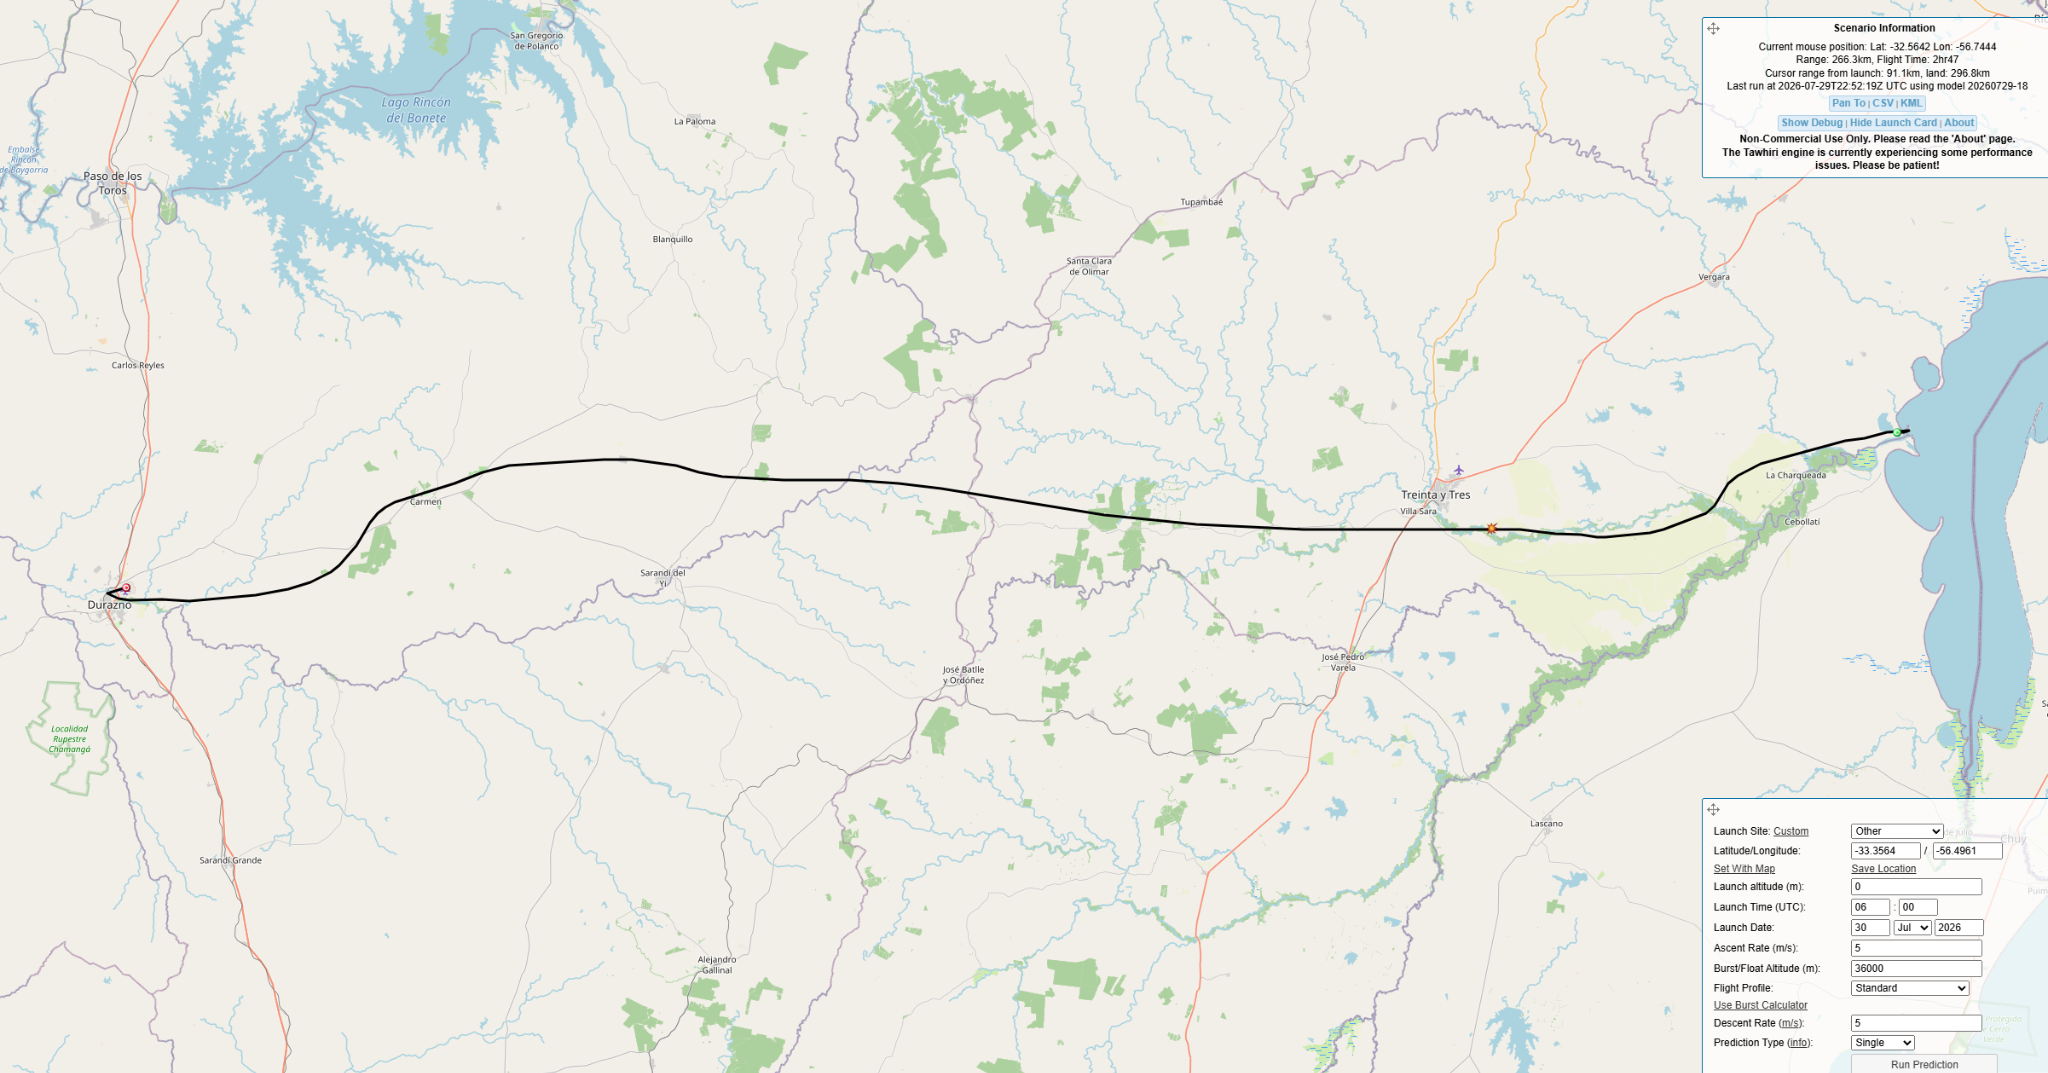
\includegraphics[width=\linewidth,keepaspectratio]{./imagenes/image50.png}

\cite{ref17,ref19,ref20,ref32} también confirman una distancia recorrida posible por arriba de los 100 km. Como la telemetría se debe recibir durante todo el trayecto, en base a las predicciones, se estima una distancia máxima de transmisión de 250 km. Aunque las predicciones establecen más distancia, se va a restringir la distancia recorrida para que no se vaya del país. En el caso del video, idealmente la transmisión solo se da en una ventana dentro de la estratosfera, es decir, aproximadamente a los 12 km de altura debe comenzar a transmitir. Según \cite{ref38} demora aproximadamente 40 minutos en llegar a la estratosfera habiendo recorrido 40 km. Y 1 hora y 20 minutos en llegar a los 25 km de altura habiendo recorrido 100 km. En base a esto, se estimó una máxima distancia de transmisión de video de 150 km.

\subsection{Selección de bandas}\label{banda}

Una vez que se resolvió la distancia de transmisión, se determinó la banda que se utilizará para transmitir. Los enlaces son unidireccionales, desde la sonda hasta la superficie terrestre. Como se mencionó antes, los módulos LoRa operan en las bandas ISM de 433, 868 o 915 MHz. Como es muy importante asegurar que la telemetría llegue a la estación terrena, se seleccionó la banda de 433 mhz por tener la mayor propagación.

Según el Reglamento del Servicio de Radioaficionados \cite{ref41} las bandas de ATV son las siguientes:

\begin{itemize}
\item
  1240 MHz a 1246 MHz
\item
  1252 MHz a 1258 MHz
\item
  1276 MHz a 1282 MHz
\end{itemize}

En términos de propagación, no hay diferencia significativa entre las bandas, pero se seleccionó la de 1240 mhz.

\subsection{Trámites para el uso de las bandas}\label{truxe1mites-para-el-uso-de-las-bandas}

Tanto la banda de 433 MHz como la de 1240 MHz se encuentran reguladas dentro del Servicio de Radioaficionados, por lo que su utilización requiere contar con el Permiso de Radioaficionado correspondiente. Este permiso es otorgado por la Unidad Reguladora de Servicios de Comunicaciones (URSEC) \cite{ref41}. Existen tres categorías de radioaficionado: Inicial, General y Superior. Para las bandas elegidas se tuvo que obtener el de categoría ``General''.

Para ingresar al Servicio de Radioaficionados, se debió cumplir con los siguientes requisitos \cite{ref65}:

\begin{itemize}
\item
  Haber participado, dentro de los 30 días corridos anteriores a la fecha del examen, en al menos una Práctica Operativa dictada por un Radio Club Habilitado, por un Radio Club o por un radioaficionado de categoría "Superior".
\item
  Aprobar el examen de ingreso, que se rinde en una plataforma informática de la URSEC.
\end{itemize}

La Práctica Operativa se realizó con un radioaficionado (Fernando Manacorda) de categoría ``Superior'' realizando varias comunicaciones radiotelefónicas con estaciones de radioaficionados ubicados en distintos puntos del país. Se usó la banda de 40 metros. Los contactos se hicieron manejando correctamente los procedimientos operativos, usando el alfabeto fonético internacional y la identificación reglamentaria de las estaciones.

El examen teórico consta de 3 partes. La primera parte es sobre la Reglamentación de las radiocomunicaciones. La segunda es de Metodos de radiocomunicaciones; Métodos para evitar y eliminar interferencias radioeléctricas; y Seguridad de las emisiones radioeléctricas. La tercera parte de Compatibilidad electromagnética y Teoría de los sistemas de radiocomunicaciones. Cada parte estaba compuesta por 15 preguntas seleccionadas al azar de un banco de 100 preguntas por parte. Se debió completar las tres partes en un tiempo máximo de 1 hora.

Se obtuvo el Permiso de Radioaficionado de Categoría ``General'', con el Distintivo de Llamada ``CX1DPH''. Con este permiso se está habilitado a transmitir en las bandas asignadas a este servicio, entre ellas la banda de 433 mHz utilizada para la telemetría y la banda de ATV 1240 mHz para la transmisión de video.

\subsection{Link budget de video}\label{link-budget-video-100-km}

Parametros:

{\def\LTcaptype{none} % do not increment counter
\begin{longtable}[]{@{}llll@{}}
\toprule\noalign{}
\endhead
\bottomrule\noalign{}
\endlastfoot
Boltzmann's Constant & \(k\) & 1,38 & j/K 10\^{}-23 \\
Temperature Reference & \(T_{0}\) & 290 & K \\
Noise Figure RTL SDR & FRX & 4 & dB \\
Noise Figure LNA & FLNA & 0.6 & dB \\
Ganancia LNA & GLNA & 17 & dB \\
\end{longtable}
}

Calculos:

{\def\LTcaptype{none} % do not increment counter
\begin{longtable}[]{@{}
  >{\raggedright\arraybackslash}p{(\linewidth - 8\tabcolsep) * \real{0.2994}}
  >{\raggedright\arraybackslash}p{(\linewidth - 8\tabcolsep) * \real{0.1304}}
  >{\raggedright\arraybackslash}p{(\linewidth - 8\tabcolsep) * \real{0.3251}}
  >{\raggedright\arraybackslash}p{(\linewidth - 8\tabcolsep) * \real{0.1851}}
  >{\raggedright\arraybackslash}p{(\linewidth - 8\tabcolsep) * \real{0.0290}}@{}}
\toprule\noalign{}
\endhead
\bottomrule\noalign{}
\endlastfoot
Parameter & Unit & Calculation & & \\
Reference Noise & dB (mW/Hz) & 10 log10 kT0 & -173,9772292 & - \\
Total Receiver Noise & dB & 10 log10 ( FLNA + (FRX − 1)/G -1 ) & -7,488006223 & - \\
Transmit Power SDR & dBm (W) & 10 log10 PT & 0 & .+ \\
Amplifier (x2) Gain & dB & 10 log10 G & 18,5 & .+ \\
Transmit Mismatch Efficiency & dB & 10 log10 ηT & -0,1322826573 & .+ \\
Transmit Efficiency & dB & 10 log10 ǫT & -0,08773924308 & .+ \\
Transmit Antenna Directivity & dBi & 10 log10 GT & 1,534059365 & .+ \\
Path Loss & dB & 10 log10 Lp & 134,3102059 & - \\
Polarization Match Efficiency & dB & 10 log10 ǫp & -3,010299957 & .+ \\
Receive Antenna Directivity & dBi & 10 log10 GR & 13,7 & .+ \\
Receive Efficiency & dB & 10 log10 ǫR & -0,08773924308 & .+ \\
Receive Mismatch Efficiency & dB & 10 log10 ηR & -0,04364805402 & .+ \\
Bit Rate & dB(b/s) & 10 log10 rb & 61,70261715 & - \\
\end{longtable}
}

Consideraciones:

\begin{itemize}
\item
  Mismatch Efficiency: Se tomó en cuenta el SWR de las antenas que se adquirieron y construyeron.
\item
  Efficiency: Las antenas, tanto de la sonda como las de la estación terrena, estarán sujetas a tubos de plástico, por lo que las pérdidas de potencia por efecto joule son mínimas.
\item
  Polarization Match Efficiency:
\end{itemize}

Resultados:

{\def\LTcaptype{none} % do not increment counter
\begin{longtable}[]{@{}
  >{\raggedright\arraybackslash}p{(\linewidth - 6\tabcolsep) * \real{0.3955}}
  >{\raggedright\arraybackslash}p{(\linewidth - 6\tabcolsep) * \real{0.0450}}
  >{\raggedright\arraybackslash}p{(\linewidth - 6\tabcolsep) * \real{0.2653}}
  >{\raggedleft\arraybackslash}p{(\linewidth - 6\tabcolsep) * \real{0.2621}}@{}}
\toprule\noalign{}
\endhead
\bottomrule\noalign{}
\endlastfoot
Eb/N0 & dB & (sum) & 15,82476255 \\
Required Eb/N0 BER=10\^{}(−6) for QPSK & dB & & 10,5 \\
Margin & dB & Eb/N0 - Required Eb/N0 & 5,324762548 \\
\end{longtable}
}

\subsection{Link budget de telemetría}\label{link-budget-telemetruxeda-250-km}

\parte{Parte IV: Segmento de vuelo}

\section{Sistema de telemetría}\label{telemetruxeda}

A la superficie terrestre se van a transmitir dos flujos de datos de distinta naturaleza: Telemetría y Video. La función principal de la telemetría es informar el estado en el que se encuentra el globo sonda. Es importante para monitorear la sonda y, en caso de falla, poder determinar el motivo. Se tomarán medidas y transmitirán los siguientes datos:

\begin{itemize}
\item
  \textbf{Temperatura (Interna y Externa):} Medición de los niveles de calor. En altitudes elevadas, las temperaturas externas pueden caer hasta los --80 °C, mientras que internamente se monitorea para asegurar que la electrónica no falle por frío o sobrecalentamiento.
\item
  \textbf{Presión Atmosférica:} Mide la fuerza ejercida por el aire. Usada en globos para validar la altitud barométrica comparándola con los datos de GPS.
\item
  \textbf{Coordenadas GPS (Latitud y Longitud):} Proporcionan la ubicación geográfica precisa para el rastreo y la recuperación tras el aterrizaje.
\item
  \textbf{Altitud:} Distancia vertical sobre el nivel del mar. Se obtiene mediante receptores GPS y se estima a partir de modelos matemáticos basados en la presión.
\item
  \textbf{Voltaje y Corriente consumida de la Batería:} Monitoreo del banco de baterías y del suministro eléctrico para asegurar que los componentes estén operando dentro de sus límites.
\item
  \textbf{Timestamp:} Mide el momento exacto en que se toman las medidas. Es importante para tener orden y asociar la medida a un momento dado.
\item
  \textbf{Estado de Control:} El vuelo se va a dividir en fases, esta medida permite informar la fase en la que se encuentra la sonda.
\item
  \textbf{Transmisión de video:} Informar cuando comience la transmisión de video.
\end{itemize}

La telemetría se va a transmitir durante todo el vuelo, pero a cada 10 segundos. No es necesario transmitir los valores continuamente porque no suma información útil y solo demandaría de más recursos de energía, que termina impactando en costos y peso.

\subsection{Sensores}\label{sensores}

Se consideraron varios tipos de sensores, teniendo en cuenta el rango operativo de temperatura, su funcionamiento a baja presión atmosférica, el consumo energético, la precisión que tiene el sensor y el costo de adquirirlo. Además, se exploraron casos en misiones de globos estratosféricos similares a las nuestras.

\begin{itemize}
\item
  \textbf{Temperatura:}

  \begin{itemize}
  \item
    DHT22: Fabricado por Aosong Electronics, es un sensor digital de temperatura y humedad muy utilizado en proyectos. Se usa en proyectos educativos porque se considera de baja complejidad. Su rango operativo declarado es de −40 °C a +80 °C, con una precisión típica de ±0,5 °C. Ensayos experimentales hechos por Lay et al. \cite{ref3} indican que el DHT22 se congela y deja de responder exactamente a −40 °C.
  \item
    BME280: Desarrollado por Bosch Sensortec, es un sensor MEMS que mide presión, humedad y temperatura, con un rango térmico de −40 °C a +85 °C y una precisión aproximada de ±1,0 °C para temperatura. El BMP280 tiene las mismas características que el BME280 solo que además mide humedad \cite{ref9}.
  \item
    DS18B20: Desarrollado por Maxim Integrated \cite{ref5} se destaca como una solución específicamente adecuada para entornos extremos. Tiene un rango de funcionamiento de −55 °C a +125 °C, con una precisión típica de ±0,5 °C. En aplicaciones reales de globos estratosféricos, este sensor ha sido probado con éxito, siendo usado como sensor exterior en múltiples vuelos del proyecto Overlook Horizon HAB \cite{ref6}.
  \item
    SHT31: Fabricado por Sensirion, ofrece un rango térmico de −40 °C a +125 °C y una alta precisión de hasta ±0,3 °C. Está orientado a aplicaciones que requieren alta exactitud en la medición ambiental \cite{ref7}.
  \item
    PT100: Es un sensor de temperatura del tipo RTD (Resistance Temperature Detector) que tiene un rango de operación desde -200 °C hasta 850 °C, superando ampliamente lo que necesitamos para este caso. Se basa en la variación de la resistencia eléctrica \cite{ref8}. El PT100 debe estar acompañado con un RTD-to-Digital Converter para registrar la temperatura usando pines GPIO que tienen micro controladores.
  \end{itemize}
\item
  \textbf{Presion:}

  \begin{itemize}
  \item
    BME280: Con un rango de presión especificado de entre 300 y 1100 hPa \cite{ref9} serviría si solo fuéramos a una altura máxima de 9 km aproximadamente.
  \item
    BMP388: Elaborado por Bosch Sensortec, es una evolución del anterior con mejor precisión, alcanzando valores del orden de ±0,5 hPa. A pesar de esta mejora, su rango de presión sigue comenzando en 300 hPa \cite{ref10}.
  \item
    MS5607: Desarrollado por TE Connectivity, tiene un rango operativo de 10 a 1200 hPa con una precisión de ±1,5. También tiene un sensor de temperatura integrado con rango de −40 a +85 °C. Además, tiene una resolución de altura de 20 cm \cite{ref11}.
  \item
    MS5611: También desarrollado por TE Connectivity, tiene un rango operativo de 10 a 1200 hPa con una precisión de ±1,5. También tiene un sensor de temperatura integrado con rango de −40 a +85 °C. Además, tiene una resolución de altura de 10 cm \cite{ref12}.
  \end{itemize}
\item
  \textbf{GPS:} El principal desafío en la elección de un receptor GPS es que, por regulaciones, cuando superan los 18 km de altitud se desactivan \cite{ref13}:

  \begin{itemize}
  \item
    U-Blox NEO-6M: Registra altura y posición hasta los 160000 FT (48768 m). Para evitar que se desactive a los 18 km, debe estar en el ``Flight Mode'' (Mode 7) configurado por software \cite{ref13}.
  \item
    NEO-M8N
  \end{itemize}
\item
  \textbf{Corriente y Voltaje:}

  \begin{itemize}
  \item
    INA226: Desarrollado por Texas Instruments, mide corriente y voltaje. Utiliza un ADC para medir el voltaje y aplica el principio del Shunt con una resistencia 0.01 para medir el la corriente con la caída de voltaje que pasa por ella. La resistencia R010 permite medir un máximo de 8A, suficiente para lo requerido. De voltaje mide como máximo 36V \cite{ref95}. Su temperatura de operación se encuentra entre -40 y +125 °C. Consume aproximadamente 330μA. Fue utilizado en el FossaSat-1 en 2019 \cite{ref96}.
  \end{itemize}
\end{itemize}

Para la temperatura externa, se decidió usar el PT100 debido a su rango operativo de -200 a 850 °C. Se va a acompañar de un conversor RTD a Digital MAX31865. El PT100 es el único sensor que va a estar afuera de la estructura. No se espera que la temperatura interior alcance temperaturas extremas. Para evitar problemas por diferencias de presión, la presión interior va a ser igual a la exterior en todo momento. Esto también permite medir la presión atmosférica correctamente. Para medir la presión se decidió usar el MS5611 por su rango operativo de 10 a 1200 hPa y su resolución de altura superior al MS5607. El MS5611 también se va a aprovechar para medir la temperatura interior. Su rango de −40 a +85 °C es suficiente. Para el posicionamiento se utilizará el GPS U-Blox NEO-6M. La altura máxima que llega a registrar es más que suficiente, permite el modo que no se desactiva a los 18 km y es muy utilizado mundialmente. Para medir la corriente y voltaje se utilizará el INA226.

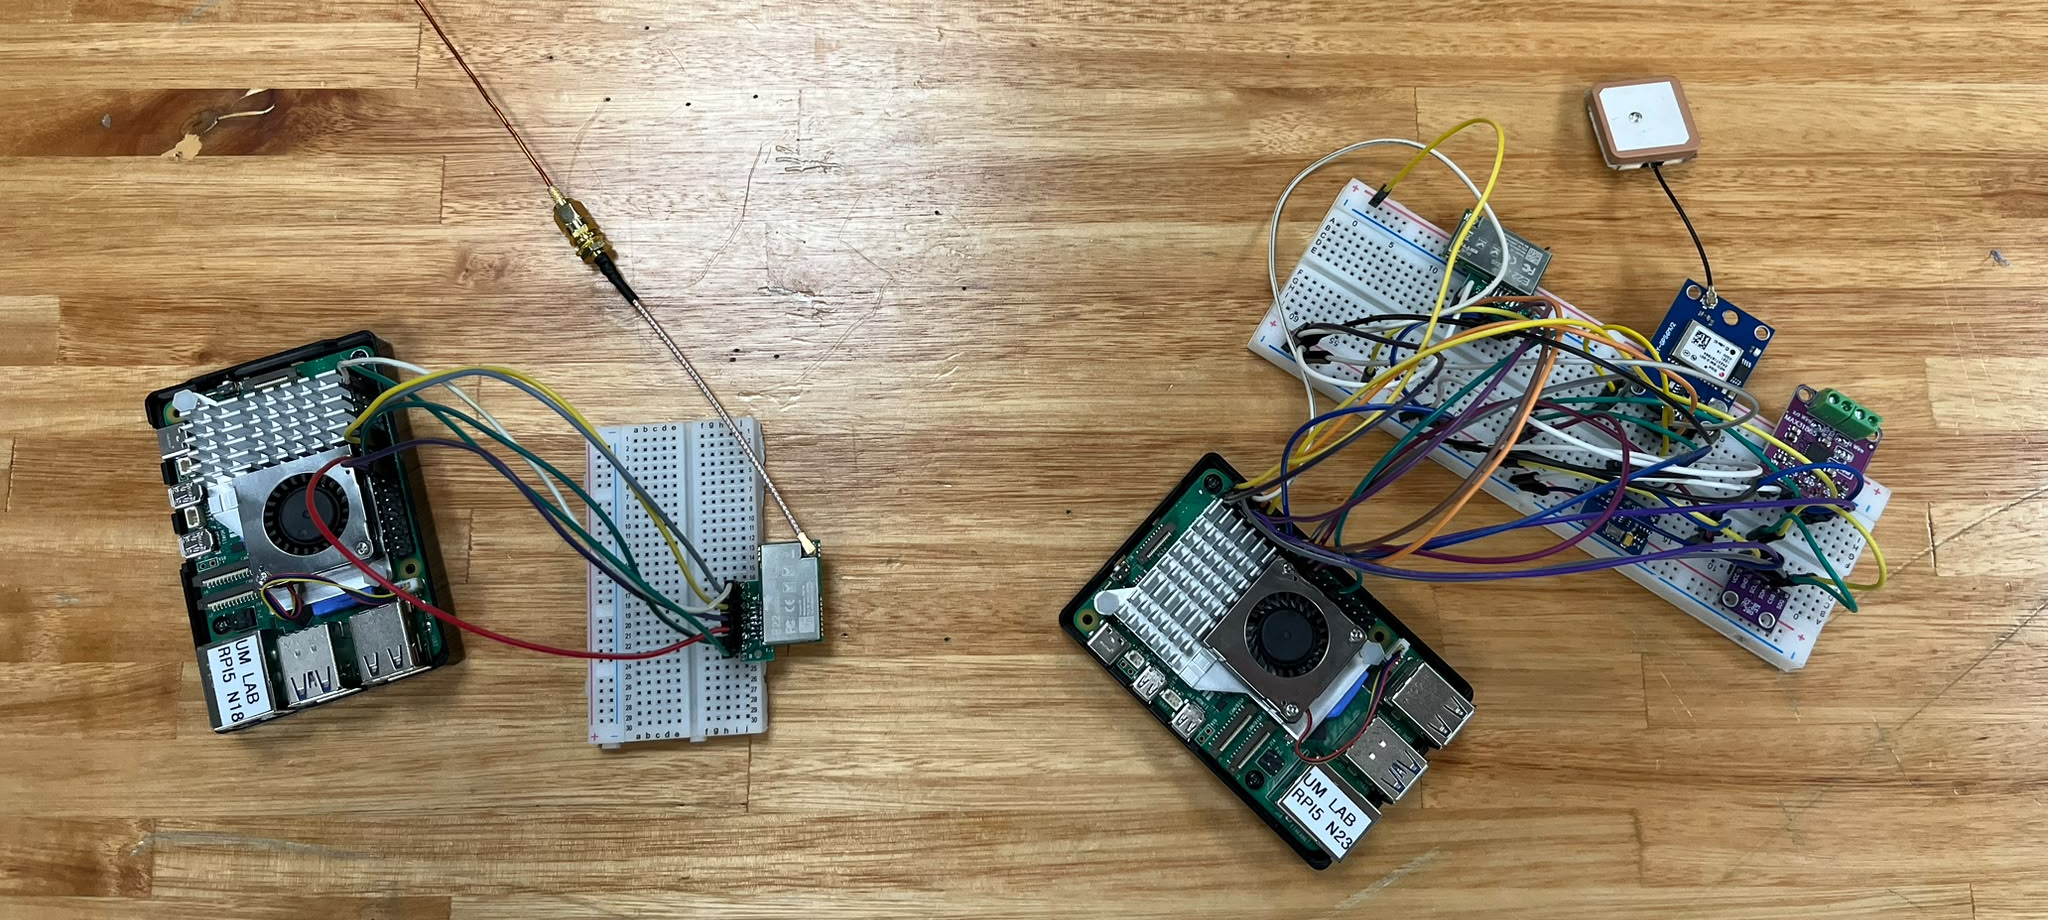
\includegraphics[width=3.6667in,keepaspectratio]{./imagenes/image59.png}

\subsection{Cantidad de bytes de telemetría a transmitir}\label{cantidad-de-bytes-de-telemetruxeda-a-transmitir}

{\def\LTcaptype{none} % do not increment counter
\begin{longtable}[]{@{}
  >{\raggedright\arraybackslash}p{(\linewidth - 6\tabcolsep) * \real{0.2926}}
  >{\raggedright\arraybackslash}p{(\linewidth - 6\tabcolsep) * \real{0.2572}}
  >{\raggedright\arraybackslash}p{(\linewidth - 6\tabcolsep) * \real{0.1801}}
  >{\raggedright\arraybackslash}p{(\linewidth - 6\tabcolsep) * \real{0.2379}}@{}}
\toprule\noalign{}
\endhead
\bottomrule\noalign{}
\endlastfoot
\textbf{Campo} & \textbf{Cantidad Caracteres} & \textbf{Bytes (UTF-8)} & \textbf{Ejemplo} \\
ID Radioaficionado & 6 & 6 & CX1DPH \\
Timestamp & 10 & 10 & 1780696364 \\
Temperatura Externa (°C) & 5 & 5 & -13.6 \\
Temperatura Interna (°C) & 5 & 5 & 25.2 \\
Presión (hPa) & 6 & 6 & 328.2 \\
Latitud & 10 & 10 & -34.883308 \\
Longitud & 10 & 10 & -56.098877 \\
Altura (m) & 9 & 9 & 23,024.50 \\
Capacidad de batería consumida (mAh) desde arranque del vuelo & 9 & 9 & 1232.1 \\
Voltaje (V) & 4 & 4 & 5.21 \\
Estado de Control & 1 & 1 & S \\
Transmisión de video & 1 & 1 & 0 \\
Delimitador & 11 & 11 & ; \\
\end{longtable}
}

Ejemplo: CX1DPH;1780696364;-13.6;25.2;1028.2;-34.883308;-56.098877;23,024.50;1232.1;5.2;S;0

Total = 78 bytes

Los estados de transmisión de video son:

\begin{itemize}
\item
  0 - No se está enviando video
\item
  1 - En menos de 5 minutos comenzará el envío de video
\item
  2 - Se está transmitiendo video
\end{itemize}

\subsection{Arquitectura Transmisión de Telemetría}\label{arquitectura-transmisiuxf3n-de-telemetruxeda}

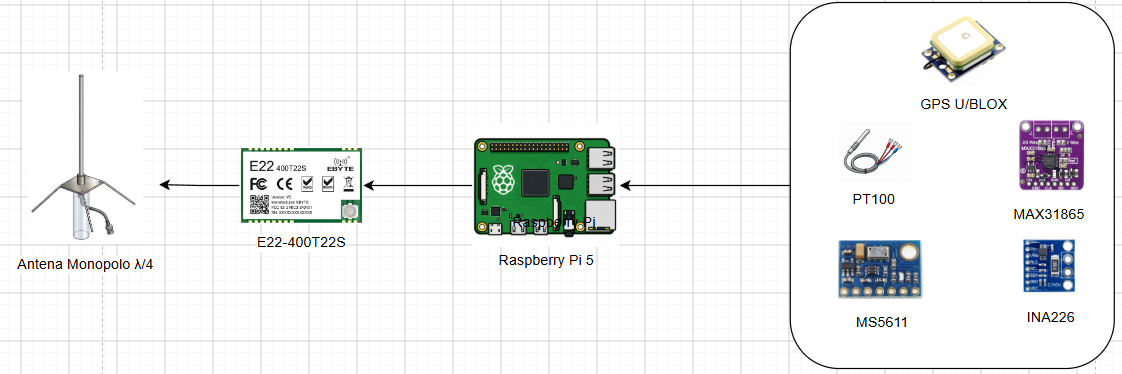
\includegraphics[width=\linewidth,keepaspectratio]{./imagenes/image60.png}

Los módulos LoRa se destacan por ser extremadamente baratos. Debido a la gran diversidad de aplicaciones IoT, existen varios tipos de módulos. Samtech desarrolló distintos chips, el más simple es el transceptor SX1262. También tienen un chip más avanzado que, además de ser un transceptor LoRa, incluye scanner de GPS y WiFi. Estos chips también se combinan con otros módulos tales como microcontroladores y bluetooth para distintas aplicaciones. Para determinar el módulo LoRa, se tomó en cuenta el rango de frecuencia de operación, la potencia de transmisión, la sensibilidad mínima, la temperatura de operación y su consumo cuando transmite. La siguiente tabla incluye los más prometedores:

{\scriptsize
\setlength{\tabcolsep}{2pt}
\renewcommand{\arraystretch}{1.15}
\hyphenpenalty=10000
\exhyphenpenalty=10000
\newcommand{\rhead}[1]{%
  \begin{minipage}[b][2.2cm][b]{\linewidth}
    \centering
    \raisebox{1pt}{\rotatebox[origin=l]{65}{\textbf{#1}}}%
  \end{minipage}}
\centering
\begin{tabular}{|
  >{\raggedright\arraybackslash}p{2.09cm}|
  >{\raggedright\arraybackslash}p{1.82cm}|
  >{\raggedright\arraybackslash}p{2.03cm}|
  >{\raggedright\arraybackslash}p{1.50cm}|
  >{\raggedright\arraybackslash}p{1.28cm}|
  >{\raggedright\arraybackslash}p{1.53cm}|
  >{\raggedright\arraybackslash}p{1.09cm}|
  >{\raggedright\arraybackslash}p{1.30cm}|
  >{\raggedright\arraybackslash}p{0.94cm}|}
\hline
\rhead{Módulo} & \rhead{Chip} & \rhead{Frecuencia} & \rhead{Potencia} & \rhead{Sensibilidad} & \rhead{Voltaje} & \rhead{Temperatura} & \rhead{Consumo TX} & \rhead{Fuente} \\
\hline
7SEMI LoRa\newline Ra-02 & SX1278 & 410--525 MHz & +20 dBm & -148 dBm & 1.8--3.3 V\newline (típ. 3.3 V) & -40 °C a\newline +85 °C & --- & \cite{ref55}\\
\hline
EBYTE LoRa\newline E22-900MM22S & SX1262 & 850--930 MHz & +21.5 dBm & -147 dBm & 1.8--3.7 V\newline (típ. 3.3 V) & -40 °C a\newline +85 °C & --- & \cite{ref56}\\
\hline
EBYTE LoRa\newline E77-400M22S & STM32WLE5\newline + SX1262 & 410--510 MHz & +21.5 dBm & -118 dBm & 1.8--3.6 V\newline (típ. 3.3 V) & -40 °C a\newline +85 °C & --- & \cite{ref19,ref58}\\
\hline
RAK5205\newline WisTrio\newline LPWAN & SX1276 & EU433, EU868,\newline CN470, US915,\newline AS923, AU915,\newline KR920, IN865 & +20 dBm & --- & 3.7--5 V & -35 °C a\newline +80 °C & 174 mA\newline (20 dBm\newline + GPS) & \cite{ref44,ref58}\\
\hline
EBYTE LoRa\newline E22-400T22S & SX1262 & 410.125--\newline 493.125 MHz & +22 dBm & -147 dBm & 2.1--5.5 V\newline (típ. 5 V) & -40 °C a\newline +85 °C & 133 mA & \cite{ref60}\\
\hline
EBYTE LoRa\newline E22-400T33S & SX1262 & 410.125--\newline 493.125 MHz & +33 dBm & -128 dBm & 2.1--5.5 V\newline (típ. 5 V) & -40 °C a\newline +85 °C & 1000 mA & \cite{ref61}\\
\hline
\end{tabular}
\par}

El módulo EBYTE LoRa E77-400M22S fue utilizado por el equipo SF-HAB \cite{ref19} en su cuarto lanzamiento para rastrear su globo. Transmitieron LoRa a +22 dBm (\textasciitilde150 mW) en 433.775 MHz a una antena ¼ de onda. Tenían 5 estaciones terrenas y el paquete más lejano que recibieron fue a aproximadamente 500 km, con el globo a 27km de altura \cite{ref19}. Tiene integrado el microcontrolador STM32WLE5 para ser programable.

\hl{El equipo del Horus Project} \cite{ref44}\hl{utilizó RAK5205 WisTrio LPWAN para transmitir la ubicación del globo a cada 3 minutos. Transmitieron en la banda 915 MHz - 928 MHz con una potencia de 50 mW. El hardware incluye GPS, sensor BME680 incorporado (presión, humedad, temperatura) y un sensor acelerómetro LIS3DH de 3 ejes. Sin embargo, es la que tiene menor potencia de transmisión.}

\hl{Se prefirió el EBYTE LoRa E22-400T22S sobre el E22-400T33S por su menor consumo energético a la hora de transmitir. Se optó por tener menos potencia de transmisión, ahorrando energía, y tener mejor sensibilidad en el receptor para compensar por la pérdida de potencia. Además, se prefirió por sobre el RAK5205 ya que tiene menor consumo energético y mayor potencia de transmisión.}

Otras tecnologías para transmitir telemetría, como APRS \cite{ref3,ref32,ref34} RTTY \cite{ref2,ref22} Sigfox \cite{ref35} son muy utilizadas en globos estratosféricos. Seleccionamos LoRa por ser una tecnología nueva y muy relevante en el mundo creciente de IoT. Además, fue muy utilizada en los proyectos estratosféricos Zephyrus \cite{ref2,ref33} respaldado por el programa Innovation to Flight del Laboratorio de Propulsión de la NASA.

\subsection{E22-400T22S}\label{e22-400t22s}

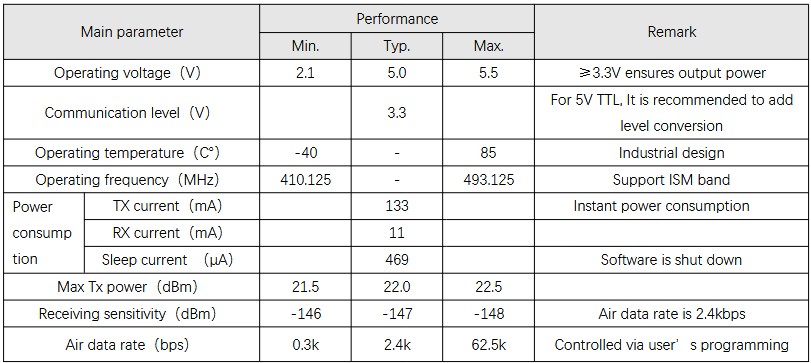
\includegraphics[width=\linewidth,keepaspectratio]{./imagenes/image65.png}

\cite{ref60}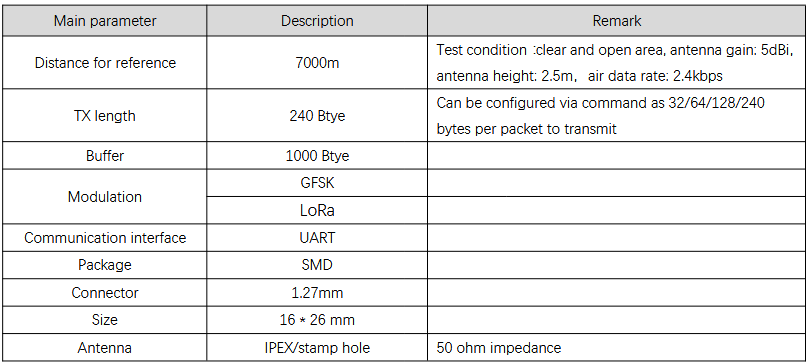
\includegraphics[width=\linewidth,keepaspectratio]{./imagenes/image42.png}

\cite{ref60} El módulo E22-400T22S solo permite modificar el Air Data Rate y con esto automáticamente ajusta los parámetros de transmisión, como el Spreading Factor, para lograr la tasa determinada. Además, tiene tamaños de paquetes configurables 32/64/128/240 y un buffer de 1000 bytes que, en caso que los datos superen el largo configurado, parte la información en distintos paquetes y usa el buffer para almacenarlos momentáneamente \cite{ref60}.

\subsubsection{PCB Adaptador}\label{pcb-adaptador}

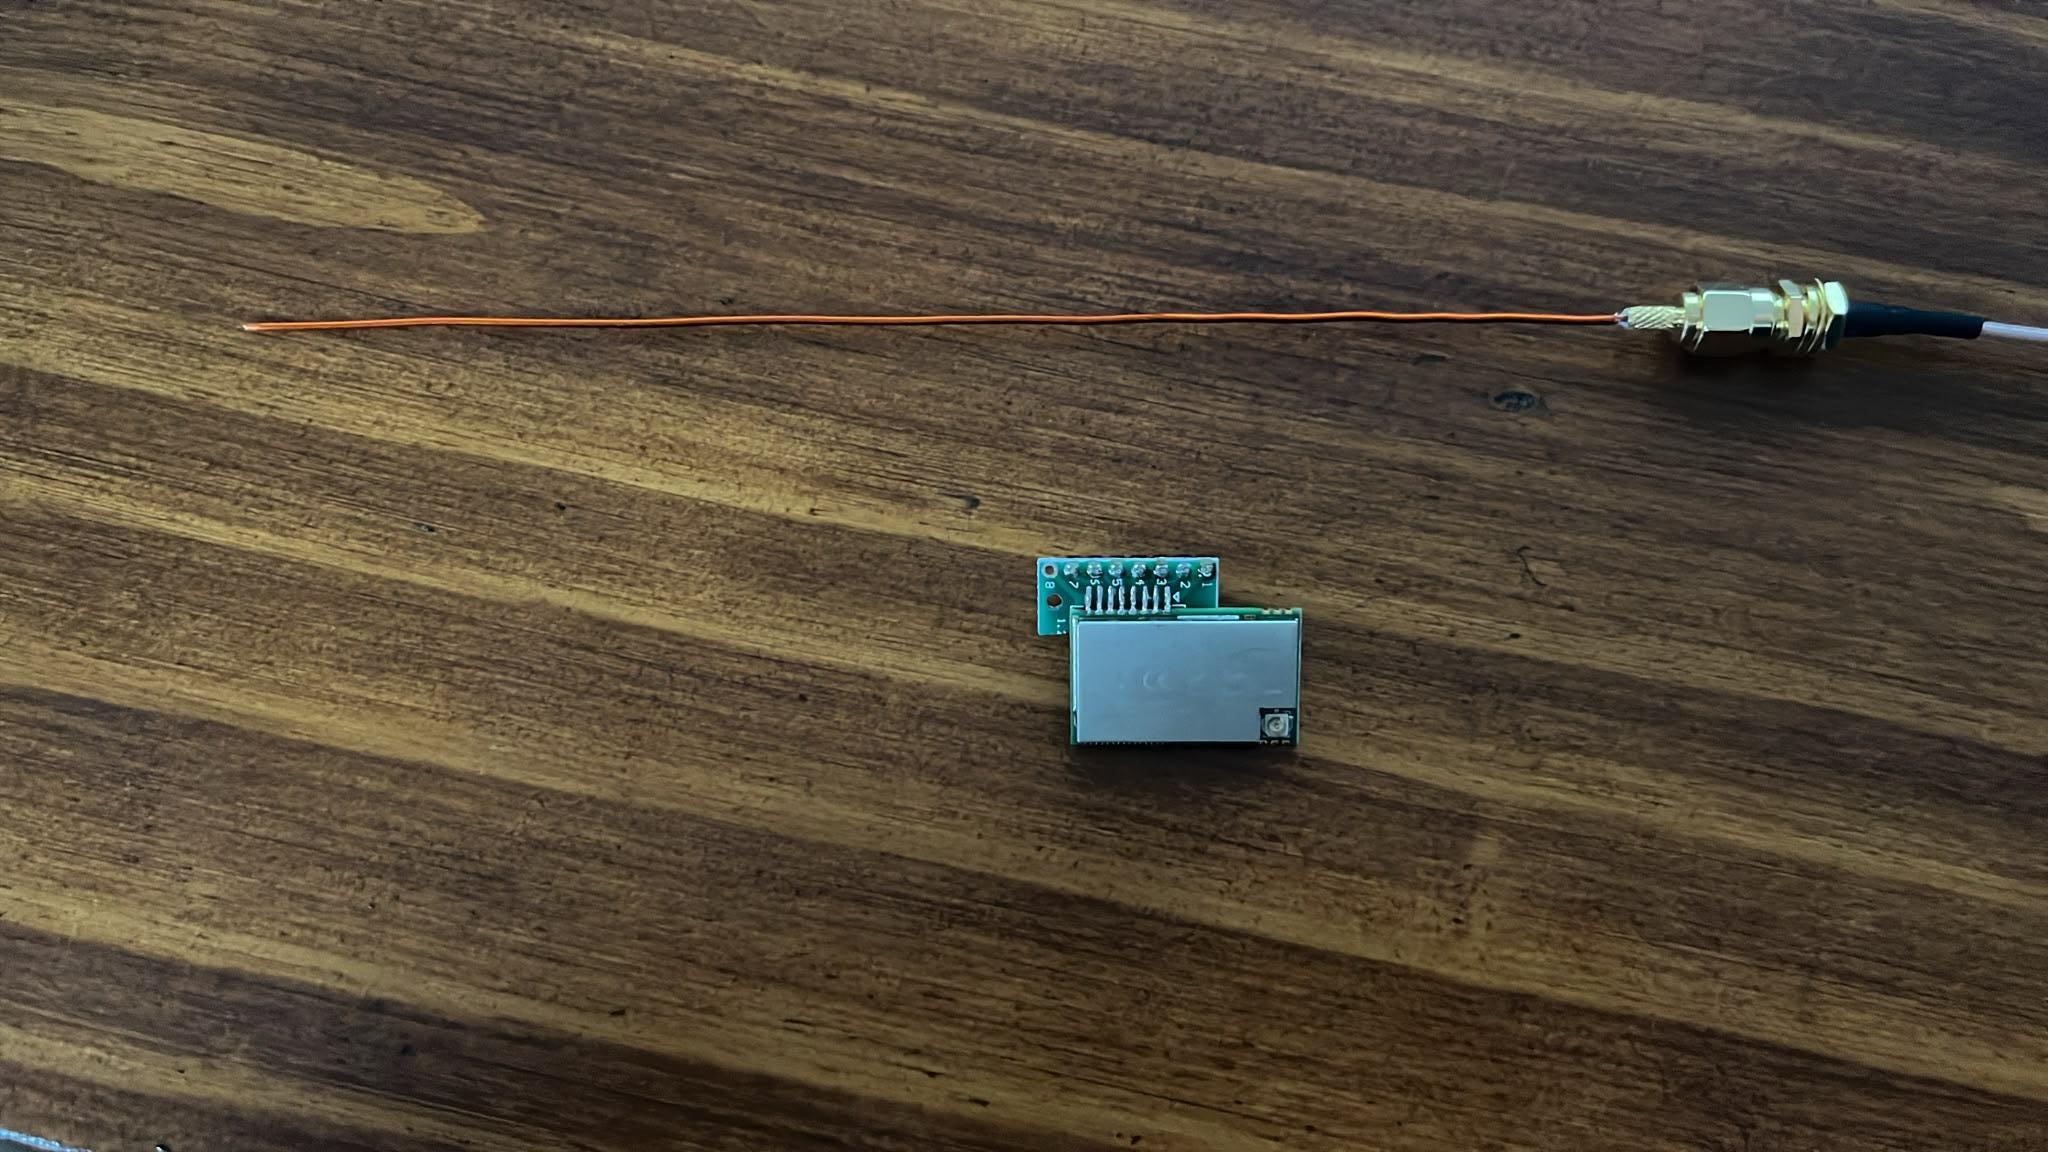
\includegraphics[width=3.6145in,keepaspectratio]{./imagenes/image51.jpg}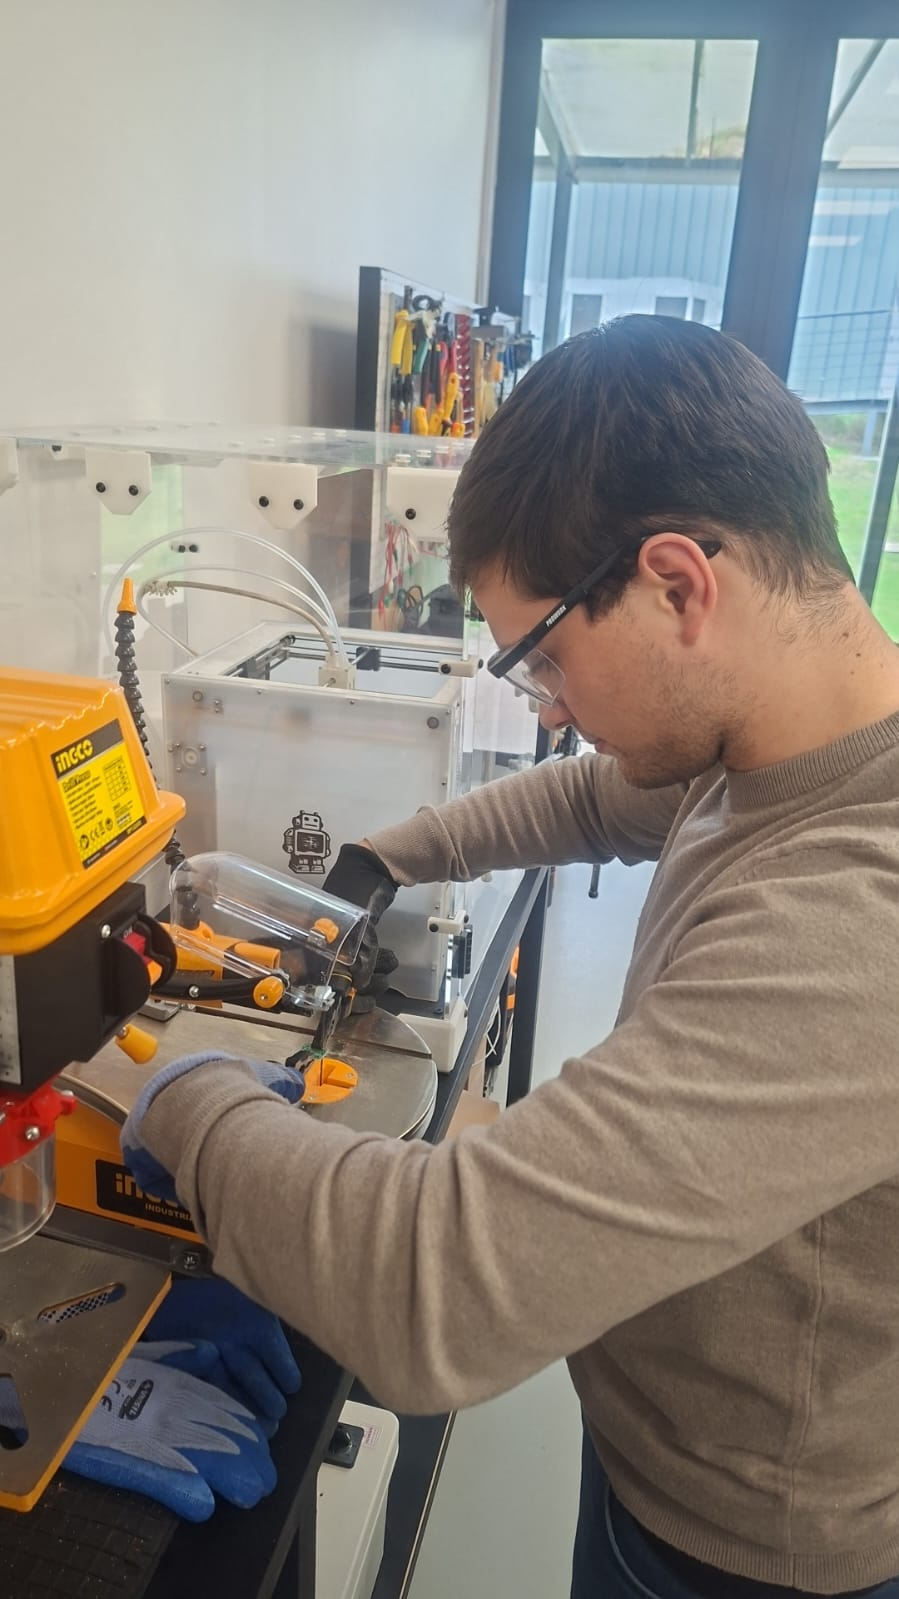
\includegraphics[width=1.7500in,keepaspectratio]{./imagenes/image80.png}

Cuando se adquirió el módulo \hl{E22-400T22S, al no tener} pines para conectarlo fácilmente con la Raspberry, se compró un PCB adaptador de SOP16 para soldar y poder conectarle pines, aprovechando el paso de 1.27 mm entre pines que tiene el módulo.

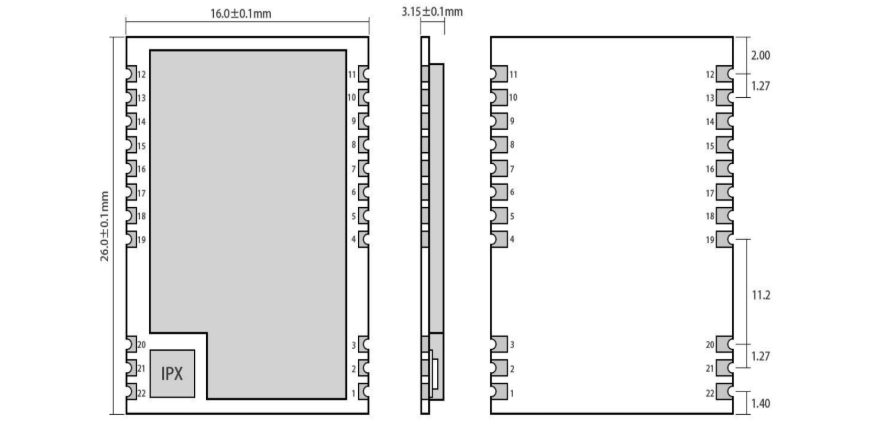
\includegraphics[width=\linewidth,keepaspectratio]{./imagenes/image45.png}

\cite{ref60}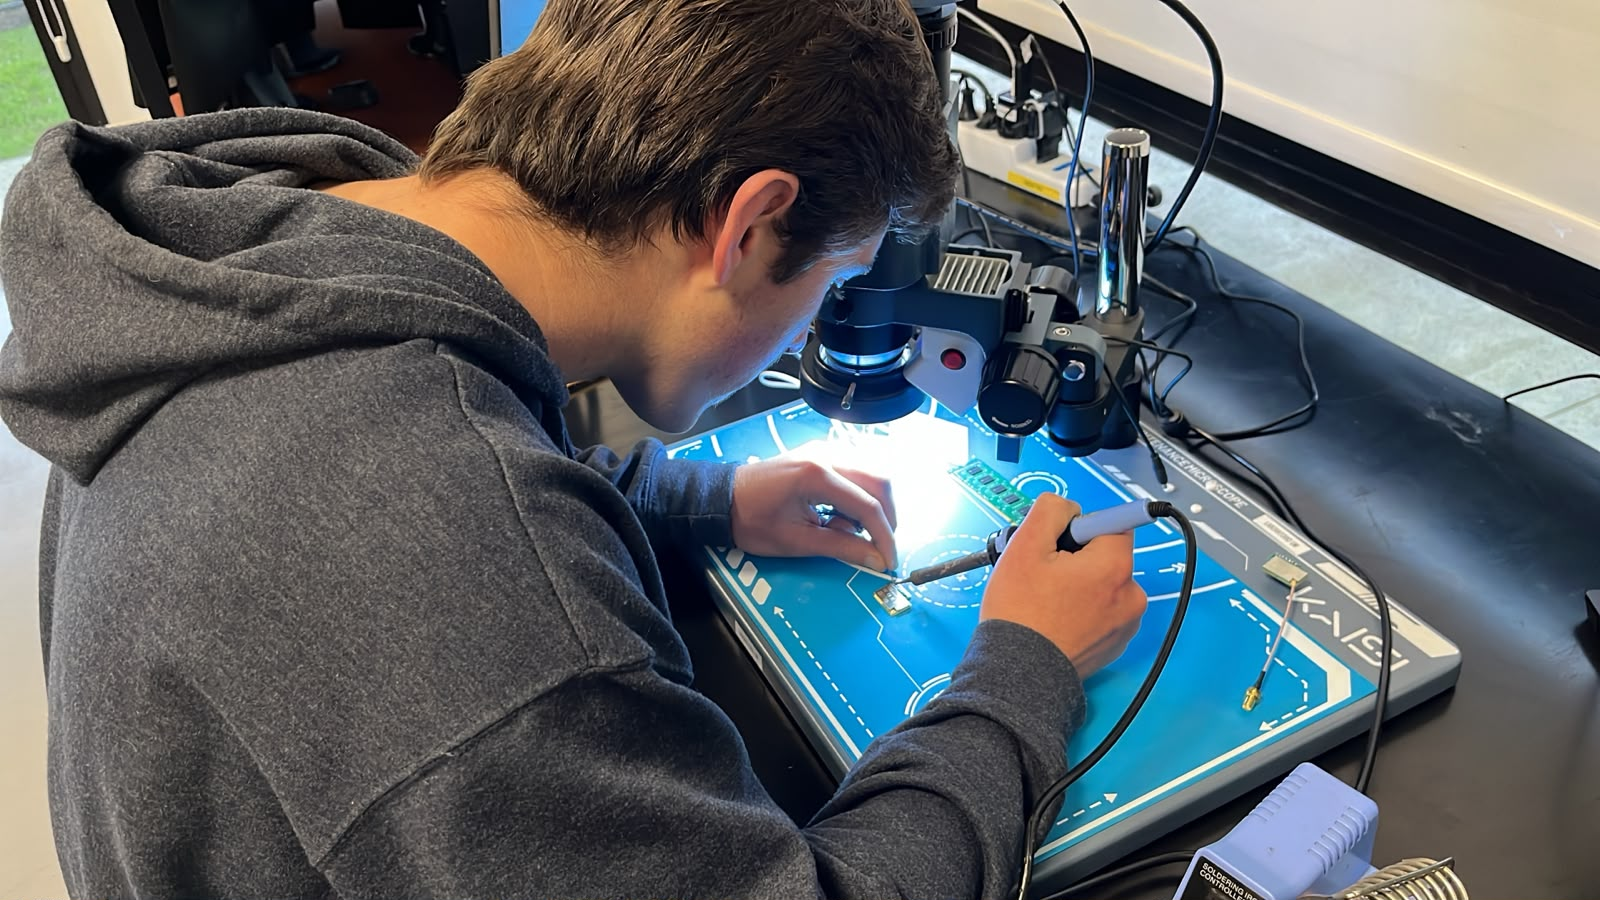
\includegraphics[width=3.2161in,keepaspectratio]{./imagenes/image81.png}

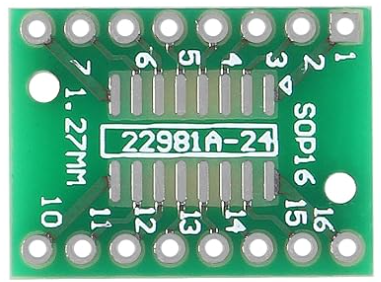
\includegraphics[width=2.5177in,keepaspectratio]{./imagenes/image38.png}

\section{Sistema de video}\label{video}


Transmitir video en tiempo real desde un globo estratosférico presenta varias dificultades teniendo en cuenta las restricciones de peso, costo, energía y ancho de banda. Además, la naturaleza del tráfico es completamente distinta a la de la telemetría.

Una de las principales restricciones que tiene el proyecto es el consumo de energía, que influye directamente en el peso del sistema. La cámara es uno de los componentes que más energía consume. Además, cuanto mayor es la calidad de video, mayor es el consumo de energía porque cada fotograma requiere de mayor procesamiento. Para este proyecto no es necesario tener una calidad de video tan alta. Transmitir video durante todo el vuelo tampoco es necesario, implica mayor consumo de energía, mayor peso y por ende mayor costo. Por lo tanto, se va a transmitir el video durante 20 - 30 minutos cuando el globo entre en la estratosfera. El objetivo principal es lograr la comunicación necesaria para uno de los tráficos de información más demandantes y poder observar la estratosfera en tiempo real.

\subsection{Cámaras}\label{cuxe1maras}

La mayoría de los proyectos similares en estos últimos años, utilizaron cámaras GoPro o cámaras RasPi. Las cámaras GoPro son reconocidas por tener un tamaño chico, son livianas y resistentes frente a golpes \cite{ref14}. Varios proyectos, como \cite{ref16,ref18,ref19,ref20,ref33} utilizaron una GoPro. Se encontraron varias opciones: GoPro Hero 5, Hero 7, Hero 8, la Insta360 One R. Todos tienen un mismo rango de operación de temperatura entre -10 °C y 35 °C \cite{ref14}. No fueron diseñadas para condiciones tan extremas, pero con algo de insolación se logra usar. De todas estas GoPro, se destacó la Hero 7 por ser la más liviana, pesando unos 116 gramos, y la más barata. La cámara también tiene una tecnología llamada HyperSmooth, que minimiza el efecto de movimientos bruscos \cite{ref15}.

Por otro lado están las cámaras RasPi. También son muy utilizadas porque son muy ligeras, compactas, baratas y graban con buena calidad. Además, son muy compatibles y fáciles de usar con las micro computadoras Raspberry Pi. Proyectos exitosos como \cite{ref2,ref17,ref21,ref22}, usaron cámaras RasPi. Se encontraron las siguientes opciones: Raspberry Pi Module 1, 2, 3, Camera Module 3 Wide, High Qualit.

Se adquirió la RasPi Module 3 por ser barata, moderna y, lo más importante, es compacta y ligera, pesando solo 4 gramos \cite{ref23}. Se descartaron las GoPro porque, a diferencia con las cámaras RasPi, son más costosas y suman más peso y complejidad al sistema. Algo que se tomó en cuenta, como menciona \cite{ref24} es que las cámaras RasPi en general pierden el foco cuando se exponen a temperaturas muy bajas.

\subsection{Soporte Cámara}\label{soporte-cuxe1mara}

Observando proyectos pasados, se ve que las cámaras tienen mucho movimiento. La sonda experimenta giros y movimientos pendulares por culpa del viento. Al comenzar el proyecto se determinó que se iba a estabilizar la cámara para minimizar el efecto de los movimientos bruscos. Durante una de las evaluaciones del peso, se descarto. El estabilizador de la cámara era unos de los componentes que más pesaba y se decidió descartar porque su función no era necesaria para cumplir con el objetivo. Se va a usar un soporte de cámara simple para tenerla asegurada contra la carcasa.

\subsection{Estándares de DTV}\label{estuxe1ndares-de-dtv}

Uruguay adoptó la versión brasileña del estándar ISDB-T (Japonés), llamado ISDB-Tb, para transmitir televisión digital desde la superficie terrestre \cite{ref59}. Existe la variante ISDB-S para transmitir ISDB vía satélite, pero, según un estudio del 2018, los estándares satelitales principales son DVB-S2 y sus variantes \cite{ref62}.

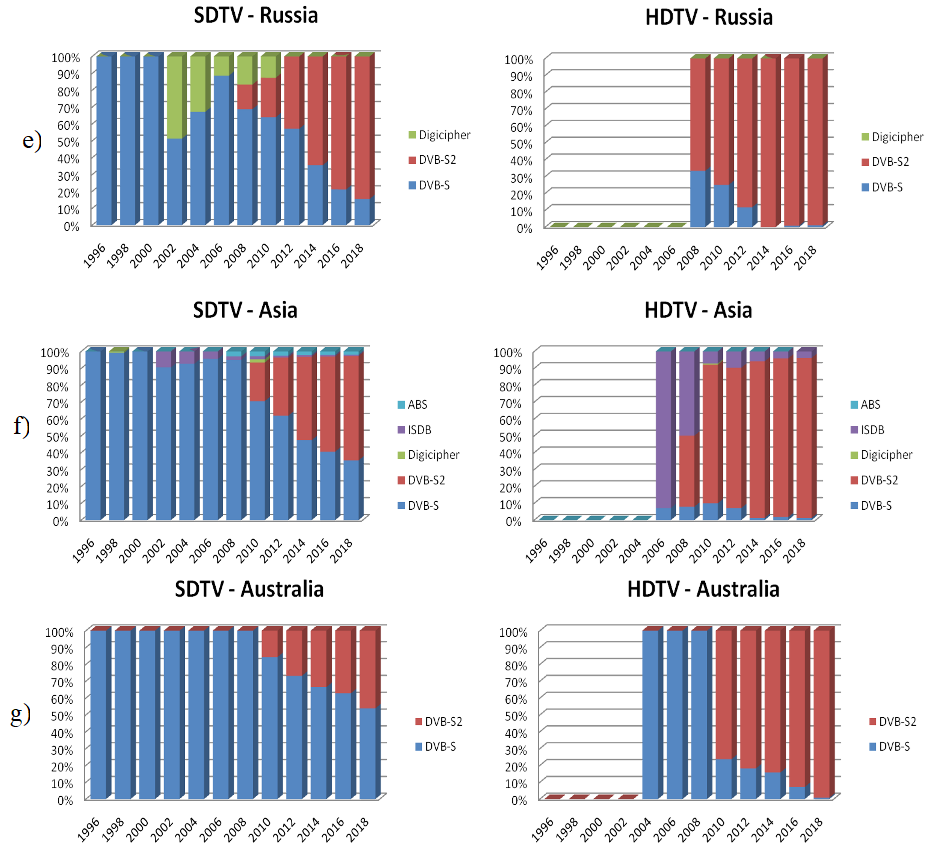
\includegraphics[width=2.6302in,keepaspectratio]{./imagenes/image1.png}

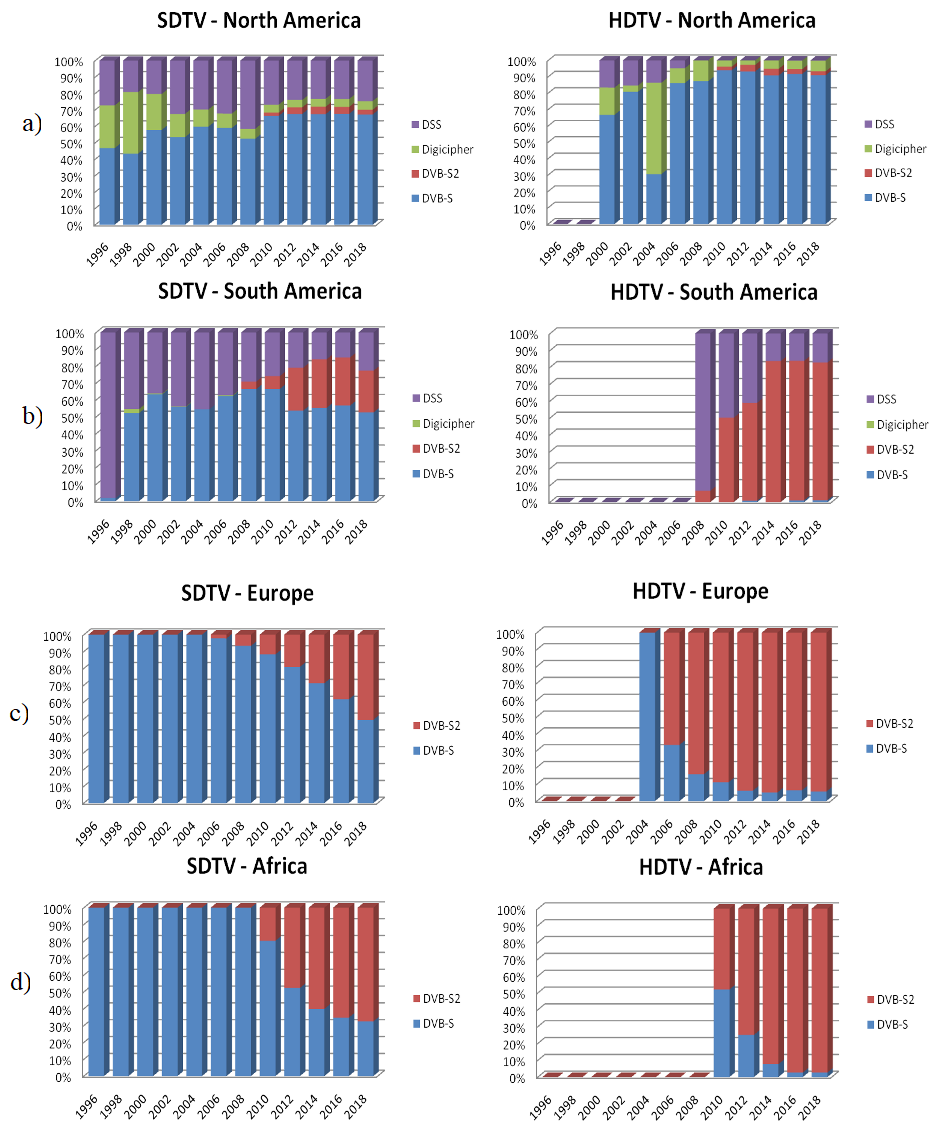
\includegraphics[width=2.7279in,keepaspectratio]{./imagenes/image4.png}\cite{ref62}\subsection{6.4 Ancho de canal de transmisión de video}\label{ancho-de-canal-transmisiuxf3n-de-video}

El CODEC es uno de los componentes que mayor procesamiento requiere por tener que disminuir el tamaño del video en tiempo real. Cuanto mayor sea la calidad del video, mayor es el procesamiento. Esto se traduce en major consumo energético, en peso y costo. El objetivo es poder observar el entorno con suficiente claridad. Después de pruebas con la cámara y observando videos con distintas calidades, se determinó la calidad de 720x480 pixeles a 30 fps cumple con nuestras necesidades.

El bitrate del video en tiempo real se calcula con la siguiente fórmula \cite{ref45}:

\(R_{video}\  = width \times \ height\  \times \ fps \times \ bpp\)

Según \cite{ref45} un valor de \emph{Bits Per Pixel} típicamente varía entre 0.05 y 0.15, dependiendo de la cantidad de movimiento entre las capturas. Cuando más movimiento hay, mayor es el BPP. La cámara va a tener un movimiento considerable. La estructura tiende a girar y oscilar en forma de péndulo. Como el peor de los casos, se toma un BPP de 0.15.

\(R_{video}\  = 720\  \times \ 480\  \times \ 30\  \times \ 0.15\  = 1.555.200\ bps\ \)

Tomando en cuenta el overhead que tienen los paquetes de Transport Stream, el cual es un 10\% adicional en promedio \cite{ref46}:

\(R_{video + TS}\  = 1.555.200\  \times \ 1.1\  = 1.710.720\ bps\)

La modulación más robusta que tiene DVB-S2 es QPSK. Permite transmitir 2 bits por símbolo y presenta una buena inmunidad al ruido. Las cuatro fases posibles se encuentran suficientemente separadas en el diagrama de constelación, reduciendo la probabilidad de error en la detección de símbolos. En comparación con modulaciones QAM de mayor orden, como 16-QAM o 64-QAM, QPSK transmite menos bits por símbolo, pero es más robusta frente al ruido y a las interferencias. Para el sistema, es importante un enlace robusto frente a interferencias debido a la distancia que se quiere alcanzar con potencia limitada.

Para calcular la tasa de símbolos, se debe tomar en cuenta los 2 bits por símbolo de QPSK y la corrección de errores \cite{ref48}. El parámetro FEC representa la relación entre bits útiles y bits totales transmitidos. Para maximizar la robustez del enlace frente a interferencia, sin sacrificar la tasa de datos del video, se toma ½ como FEC.

\(R_{S} = R_{b}/(m \times FEC\ )\  = 1.710.720/(2 \times 0.5)\  = \ 1.710.720\ sym/s\ \)

Por último, el ancho de canal se calcula con lo siguiente \cite{ref42}:

\(B\  = \ \ \)\(R_{S}\  \times \ (1\  + \ \alpha)\)

Alpha es el \emph{Roll-off Factor.} DVB-S2 permite los valores de 0.35, 0.25 y 0.2. Un valor bajo mejora la eficiencia espectral, mientras que un roll-off alto ofrece mayor robustez frente a ruidos de fase y distorsiones \cite{ref42}. Suponiendo que se tome 0.35, usando los resultados anteriores, se obtiene el máximo ancho de canal necesario:

\(B\  = \ \ \)\(1.710.720\  \times \ (1\  + \ 0.35)\  = \ 2.31\ Mhz\)

\subsection{Arquitectura de transmisión de video}\label{arquitectura-transmisiuxf3n-de-video}

Según \cite{ref40} el sistema de transmisión se compone de un transmisor, seguido de un filtro pasabanda, seguido de otros componentes como amplificadores, splitters, entre otros, y finalizado con la antena.

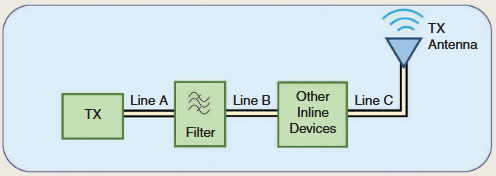
\includegraphics[width=5.1667in,keepaspectratio]{./imagenes/image70.png}

\cite{ref40} La arquitectura inicial es la siguiente:

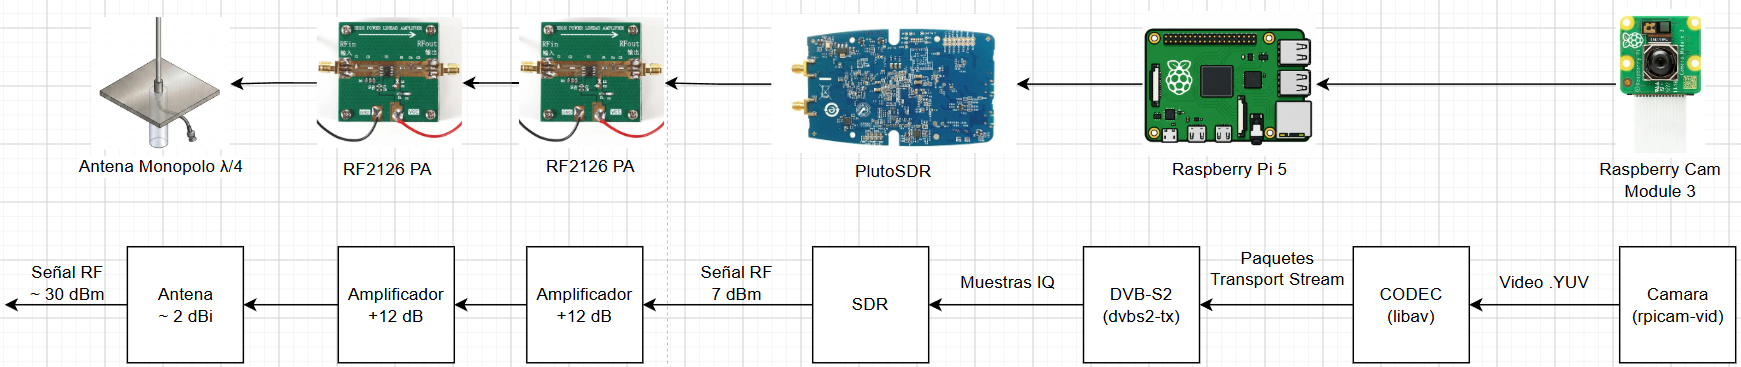
\includegraphics[width=\linewidth,keepaspectratio]{./imagenes/image89.png}

\subsubsection{Transmisor}\label{transmisor}

Debido a restricciones de tiempo, costo y conocimiento se decidió investigar Radios Definidos por Software para resolver la transmisión de video.

\cite{ref43} \hl{destaca dos plataformas de hardware SDR populares con capacidad TX:}

\begin{itemize}
\item
  \hl{PlutoSDR: Un transceptor autónomo capaz de transmitir y recibir simultáneamente (full duplex), muy utilizado en entornos académicos y de desarrollo.}
\end{itemize}

\begin{itemize}
\item
  \hl{HackRF One: Un dispositivo de half duplex conocido por su amplio rango de frecuencia (de 1 MHz a 6 GHz) y su robusto soporte comunitario.}
\end{itemize}

\hl{El equipo del Horus Project} \cite{ref44} \hl{construyó un Globo de Gran Altitud basado en el estándar DVB-S1. Utilizaron un Raspberry Pi Zero W para capturar y comprimir el video, seguidamente modulada y transmitida por un LimeSDR Mini y potenciada con un amplificador LDMOS. Logrando recibir video a casi 190 km.}

Para transmitir el video, se adquirió un ADALM-PLUTO SDR\hl{. De los tres SDR, era el más económico y disponible para comprar.} 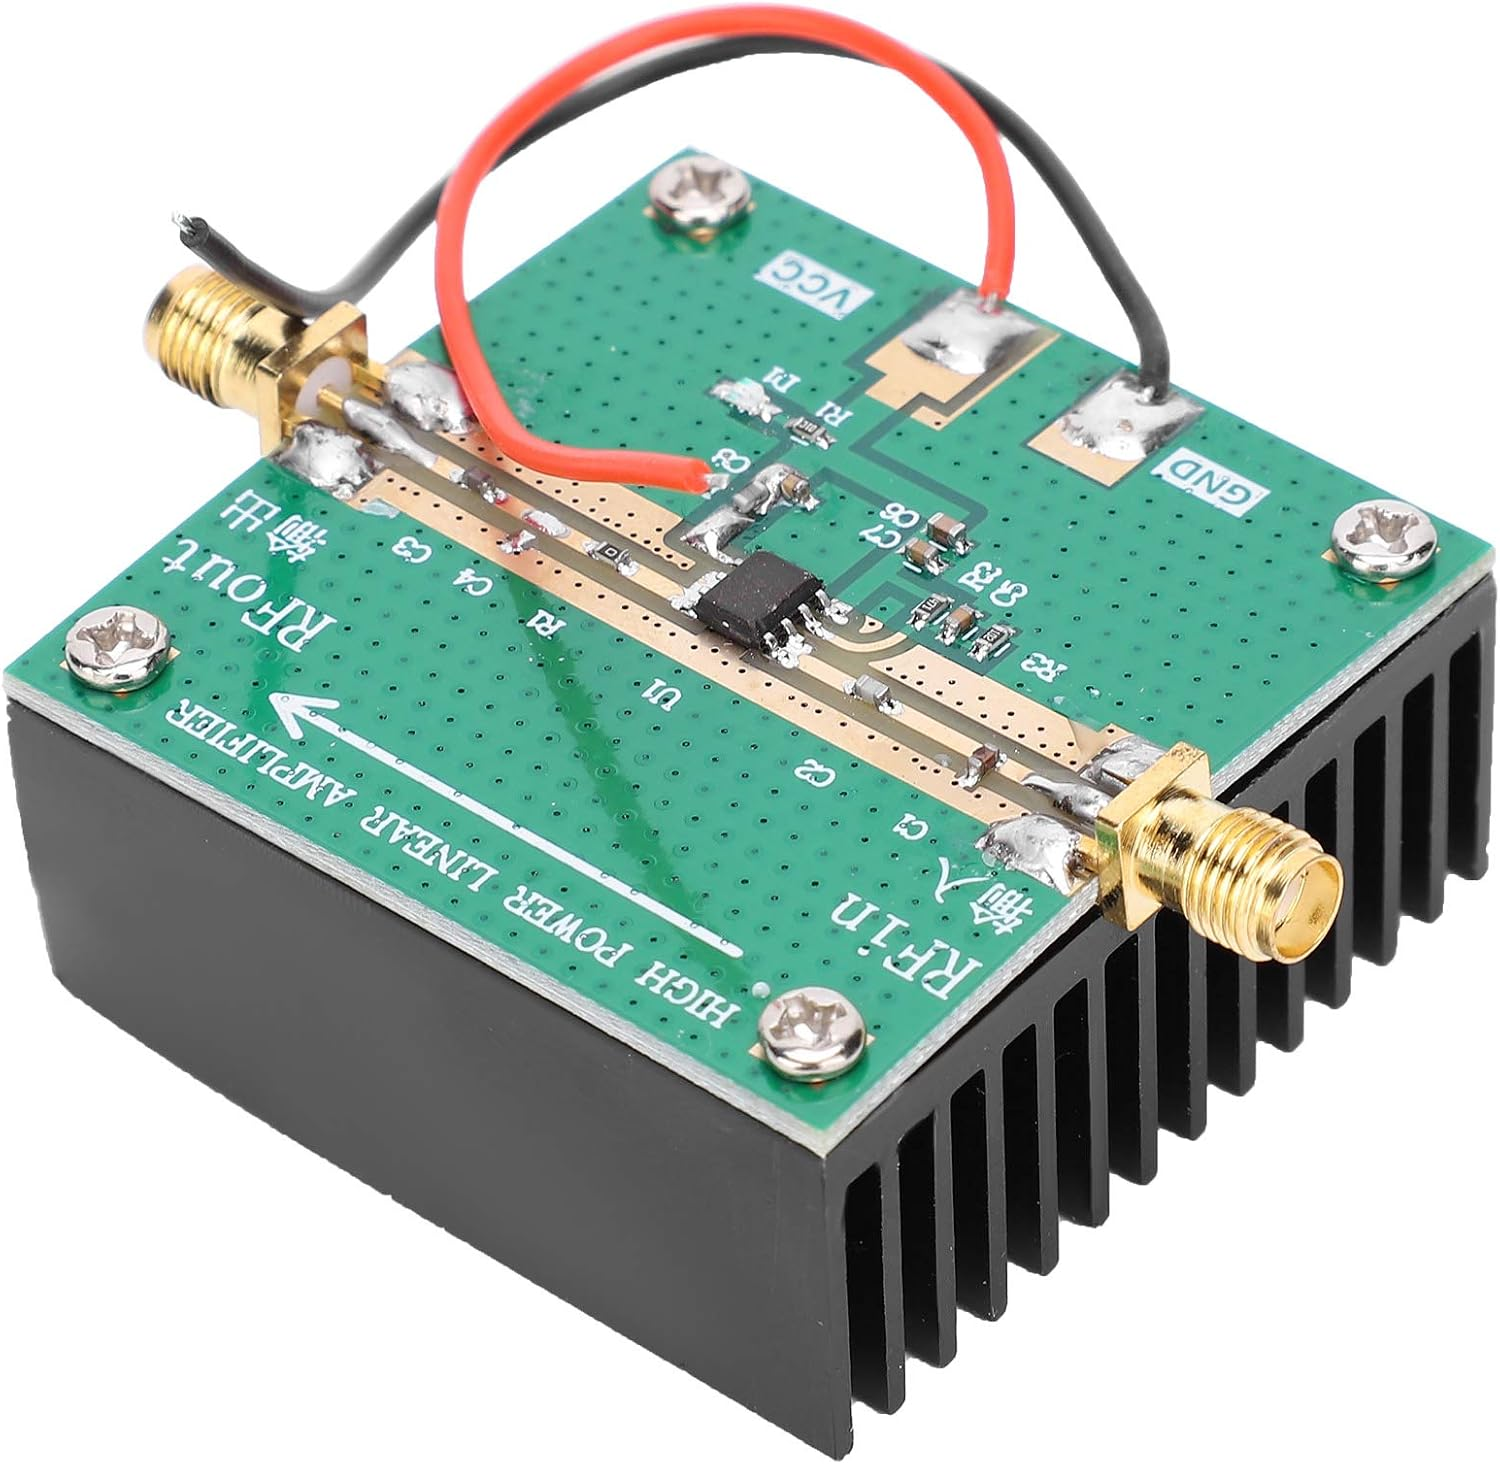
\includegraphics[width=2.0469in,keepaspectratio]{./imagenes/image26.jpg}

\subsubsection{Amplificador de Potencia}\label{amplificador-de-potencia-1}

Se adquirió el amplificador de potencia RF2126:

\begin{itemize}
\item
  Ganancia: 12 dB
\item
  Eficiencia: 45\%
\item
  Lineal
\item
  Frecuencia de Operación: 400 - 2700 mhz
\item
  IM3: 24 dBm
\item
  Máxima Potencia de Entrada: 20 dBm
\item
  Voltaje de Alimentación: 3 - 6 V
\item
  Temperatura de Operación: -40 a +125 °C
\item
  Corriente de Alimentación: 450 mA
\item
  Corriente de Alimentación Inactivo: 180 mA
\item
  Potencia Máxima de Salida: 29 dBm (VCC=4.8V, PIN=+19dBm, Freq=2450MHz)
\item
  Impedancia: 50 ohm
\end{itemize}

En principio se decidió poner dos RF2126 en serie con 6 dBm de potencia de entrada para que salgan aproximadamente 30 dBm. Se utilizó un medidor de potencia para verificar la ganancia y resultó que para 1240 mhz, solo sumaba 10 dB de ganancia. Además, uno de los que recibió estaba roto. A partir de esto, se decidió invertir en un amplificador con una ganancia de aproximadamente 20 dB y P1dB de 20 dBm, de un proveedor confiable, para ponerlo antes del RF2126. Así llegar a transmitir con aproximadamente 30 dBm.

Entonces, se adquirió el amplificador de potencia ZX60-V63+. En 1240 mhz: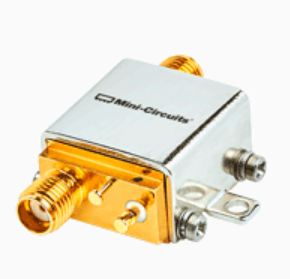
\includegraphics[width=2.2708in,keepaspectratio]{./imagenes/image78.png}

\begin{itemize}
\item
  Ganancia: 20.9 dB
\item
  IP3: 32.3 dBm
\item
  Frecuencia de Operación: 50 - 6000 mhz
\item
  Máxima Potencia de Entrada: 13 dBm
\item
  Voltaje de Alimentación: 5V
\item
  Temperatura de Operación: -40 a +85 °C
\item
  Corriente de Alimentación: 78 mA
\item
  P1dB: 18.5 dBm
\item
  Impedancia: 50 ohm
\end{itemize}

Quedando la siguiente arquitectura:

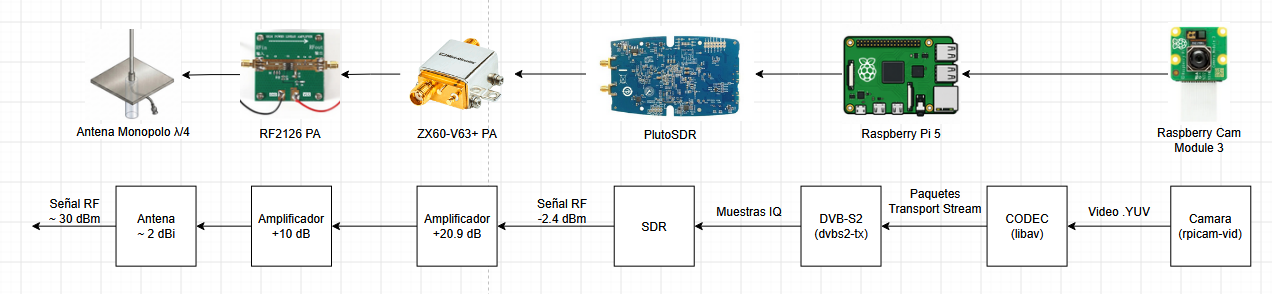
\includegraphics[width=\linewidth,keepaspectratio]{./imagenes/image31.png}

Después de pruebas con el medidor de potencia, se descubrió que el amplificador RF2126 saturaba en 20 dBm, por lo que se terminó descartando.

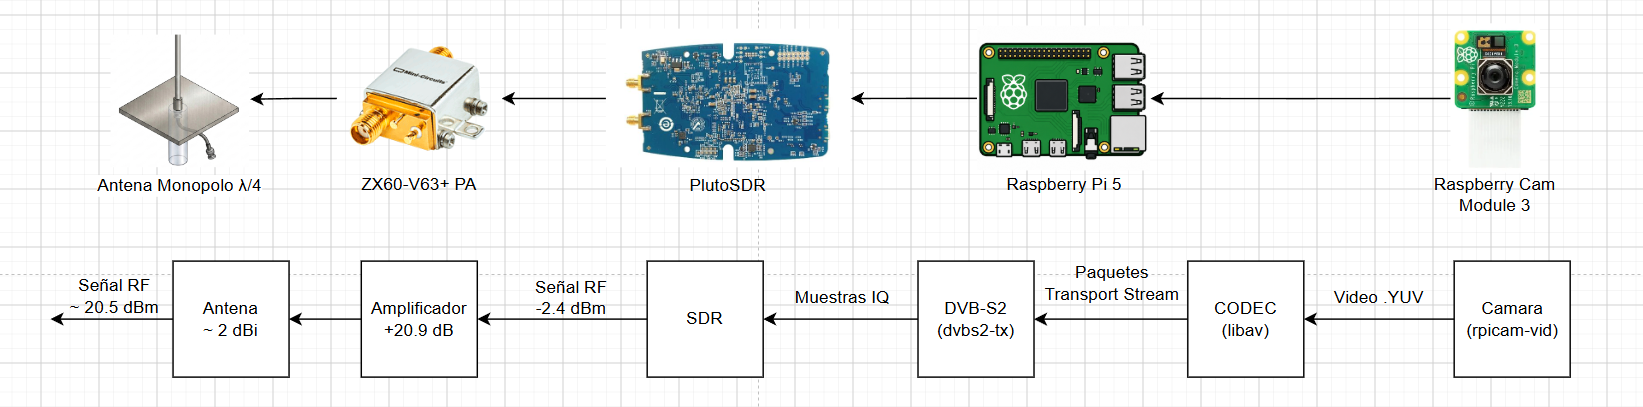
\includegraphics[width=\linewidth,keepaspectratio]{./imagenes/image93.png}

\section{Antenas de transmisión}\label{antenas-transmisiuxf3n-de-video-y-telemetruxeda}

El enlace es unidireccional, desde el globo hacia la estación terrena. En el globo, se determinó que la mejor opción es usar una antena de baja ganancia, específicamente un dipolo o monopolo. El globo gira y cambia de orientación constantemente, por lo que se necesita un patrón de radiación casi omnidireccional y ancho de haz amplio. Estas antenas son simples, muy livianas, baratas y confiables, permitiendo la comunicación sin necesidad de apuntamiento preciso \cite{ref2,ref44}.

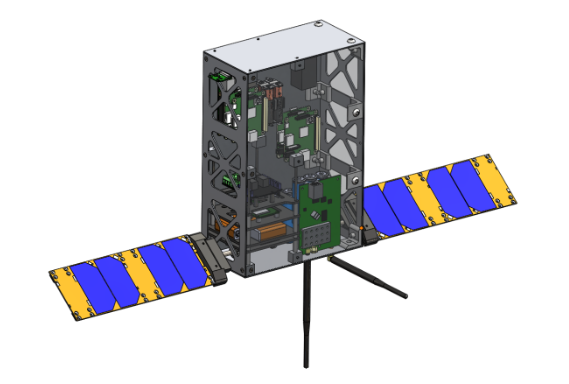
\includegraphics[width=3.3741in,keepaspectratio]{./imagenes/image77.png}

\cite{ref44} Se prefirio un monopolo debido a la forma geométrica que tiene. Una antena monopolo es un radiador vertical que representa "una mitad" de un dipolo, utilizando la tierra o un sistema de cables (radiales) como plano de referencia para actuar como la otra mitad. El diseño más común es el que mide un cuarto de la longitud de la onda que se quiere transmitir. Su parámetro más crítico para la eficiencia es el sistema de tierra. La tierra actúa como un "espejo" eléctrico que completa la antena. Si el sistema de tierra es pobre, gran parte de la potencia del transmisor se desperdiciará en forma de calor, se altera la impedancia y por ende se desajusta la Relación de Onda Estacionaria. Además, se degrada el patrón de radiación \cite{ref70}.

En caso de usar radiales como plano de tierra, se recomienda utilizar de 3 a 4 radiales que midan también un cuarto de la longitud de onda. En el proyecto GLOBOSAT01 se utilizaron 3 elementos radiales \cite{ref71}. Un monopolo de λ/4 sobre un plano de tierra tiene una impedancia cercana a 37 Ω. Al inclinar los radiales hacia abajo (monopolo vertical) unos 45 grados, la impedancia sube hacia los 50 Ω, lo que permite una conexión directa a un cable coaxial estándar con una ROE muy baja \cite{ref70}.

En caso de usar una plancha metálica y que actúe como un plano de tierra eficaz, debe tener un tamaño suficiente para "reflejar" la señal y minimizar las pérdidas. La plancha debe extenderse desde la base del radiador al menos un cuarto de longitud de onda en todas las direcciones. En este caso, no es posible modificar la impedancia para acercarla a 50 Ω por lo que se deberá de asumir un ROE de aproximadamente 1.4 o realizar otro tipo de acoplamiento \cite{ref70}.

\subsection{Construcción}\label{construcciuxf3n}

Para construir los elementos radiadores de los monopolos, se adquirieron conectores SMA y alambre de cobre de 1mm de diámetro. De esta manera se tenía una interfaz conveniente para conectar otros cables coaxiales SMA.

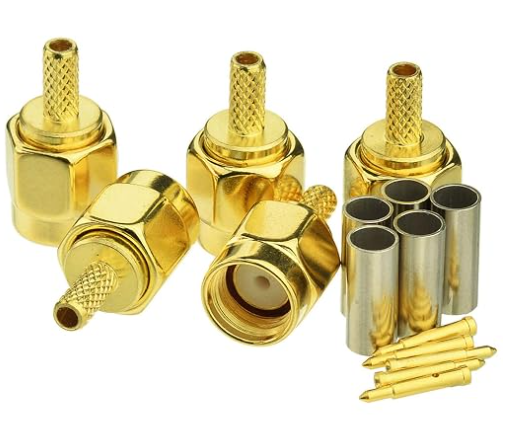
\includegraphics[width=2.2351in,keepaspectratio]{./imagenes/image54.png}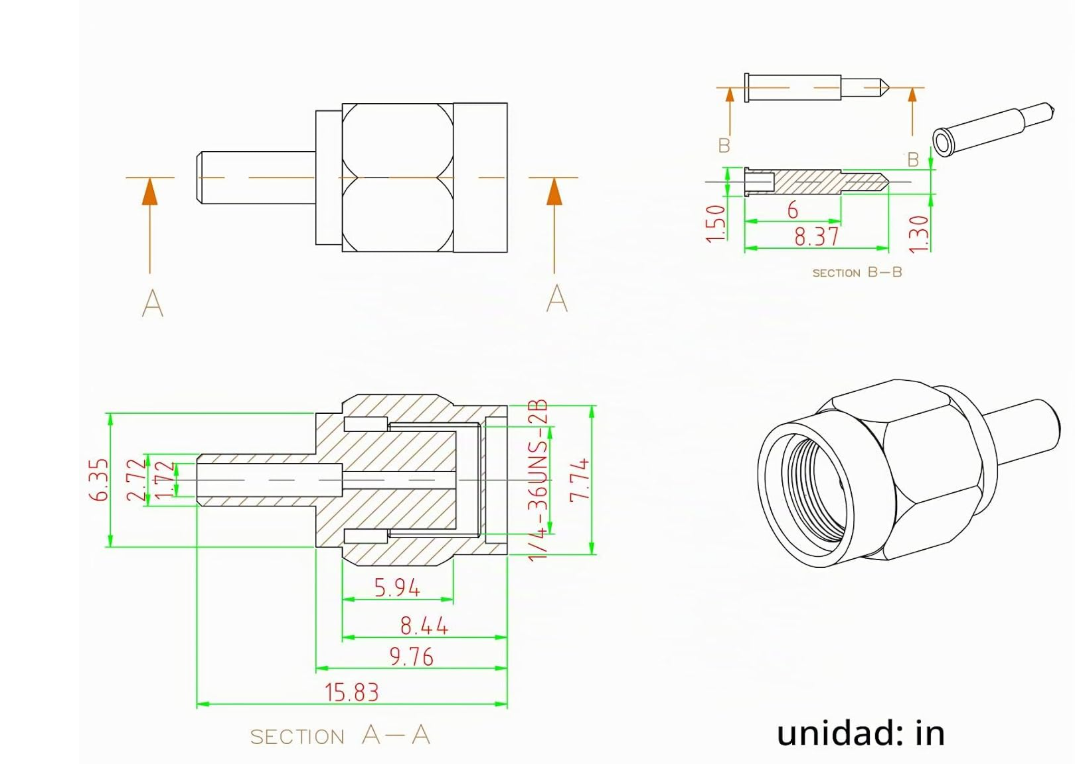
\includegraphics[width=2.7153in,keepaspectratio]{./imagenes/image25.png}

Para ensamblar, se cortó un pedazo de alambre de cobre, se redujo una parte de la punta y se insertó en la clavija del conector utilizando estaño. 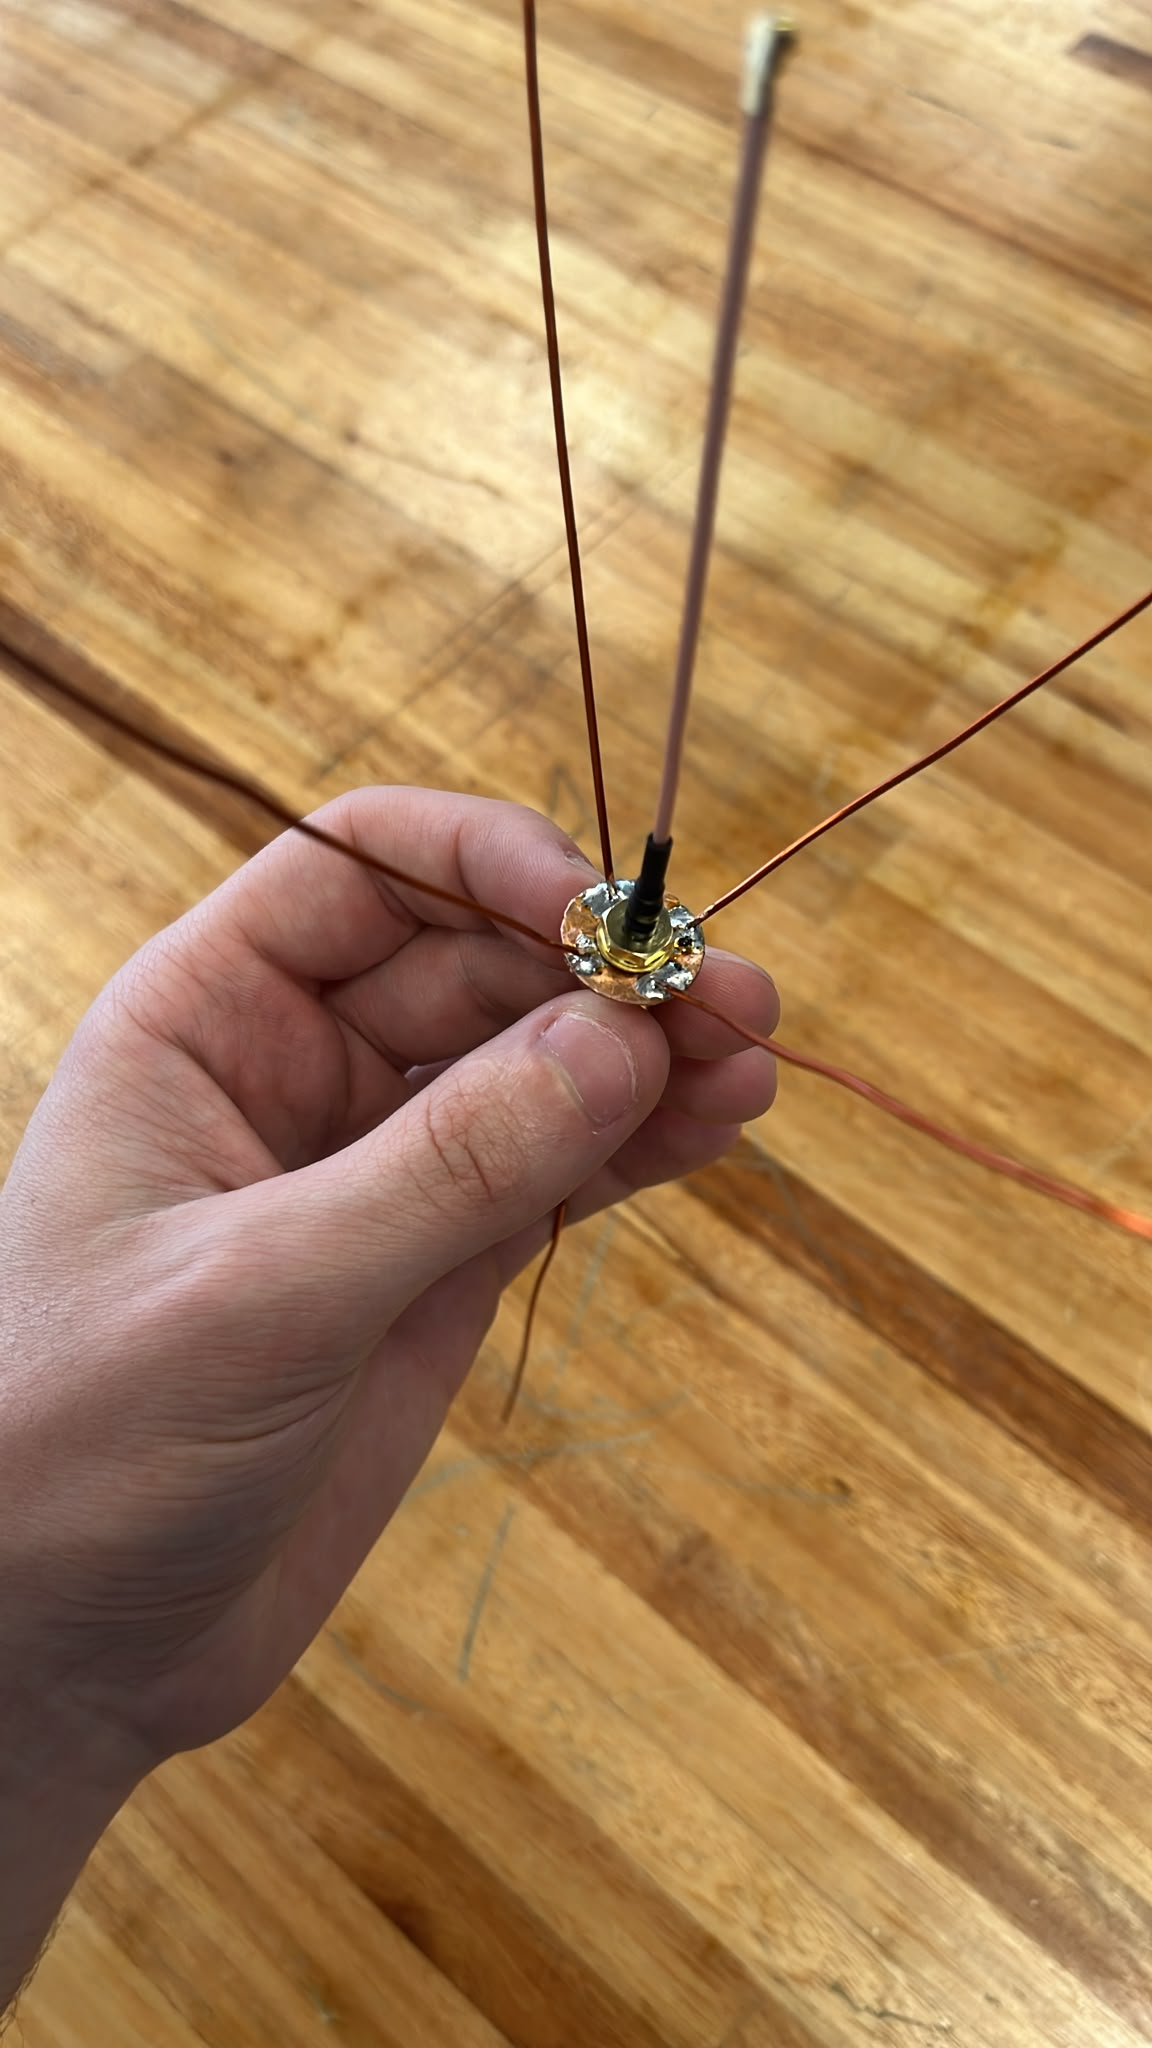
\includegraphics[width=1.6019in,keepaspectratio]{./imagenes/image67.png}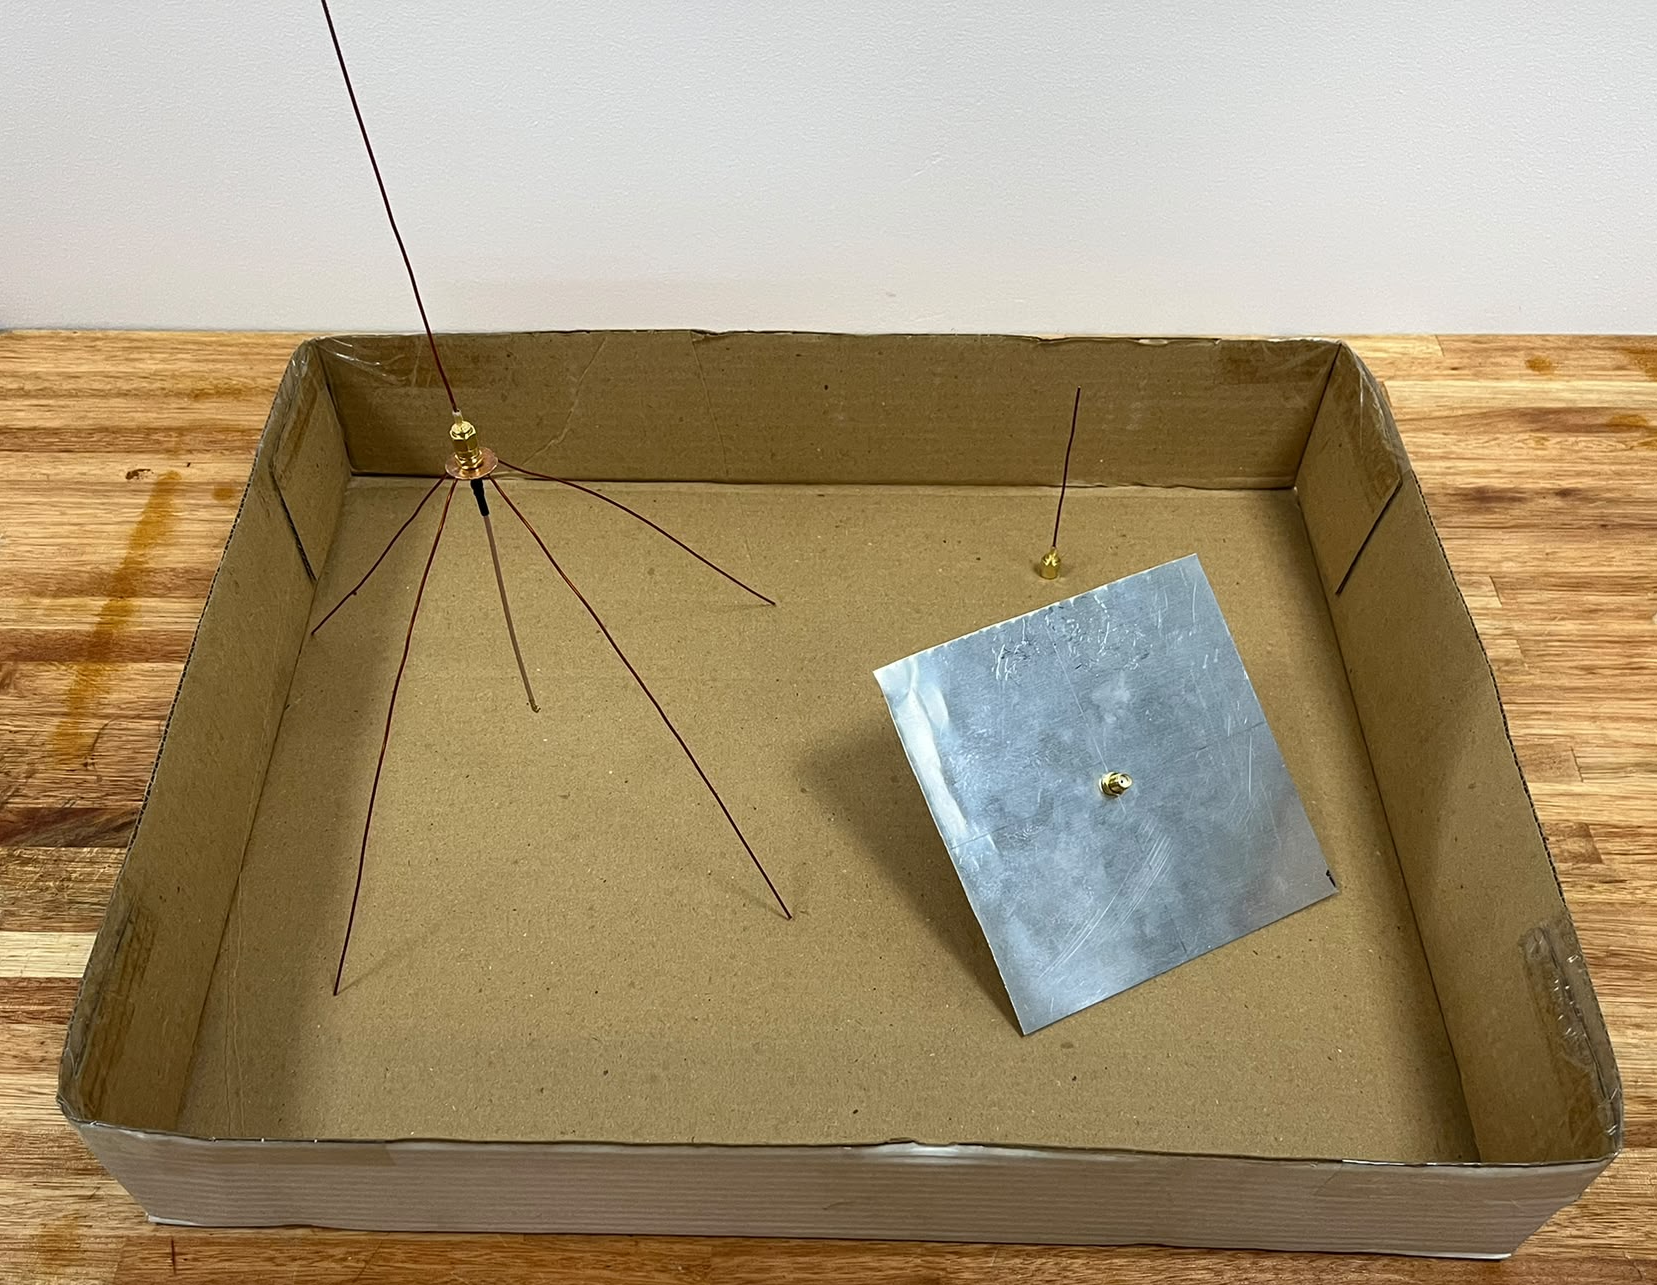
\includegraphics[width=3.6823in,keepaspectratio]{./imagenes/image73.png}

Para la antena de 433 mhz, se requirió una antena de aproximadamente 17 cm. Hacer un plano de tierra con una plancha metálica no es posible debido al tamaño, el peso y el espacio que ocupa. Se decidió que la mejor opción es utilizar radiales.

Para construir los radiales de la antena de 433 mhz se tuvo que realizar varias iteraciones. Para la primera se cortó una arandela de cobre y se le soldaron 4 radiales. Al usar cobre de 1 mm de diámetro, los radiales eran fáciles de flexionar y la soldadura no quedaba muy resistente, por lo que se rompía fácilmente. Para hacer los radiales más robustos, se cortó una arandela cuadrada y se le soldaron alambres de cobre de 2 mm de diámetro. Con esto resolvimos la flexibilidad de los radiales, pero las soldaduras seguían siendo poco resistentes.

Para la última iteración se soldaron los segmentos de alambre de cobre de 2 mm con terminales de bronce. Después, se soldaron tornillos sobre las puntas de la arandela cuadrada de cobre y se colocaron los terminales con los radiales sobre y se reforzó con más estaño. De esta manera se logró construir radiales que no sean fáciles de desprender de la arandela.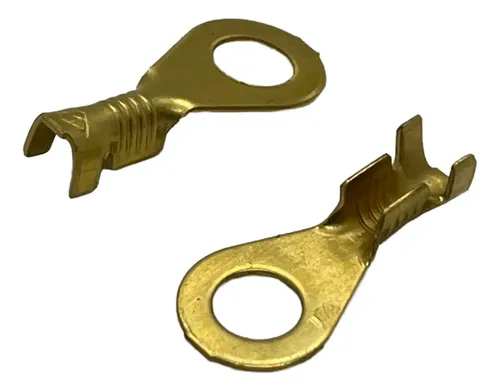
\includegraphics[width=1.7135in,keepaspectratio]{./imagenes/image3.png}

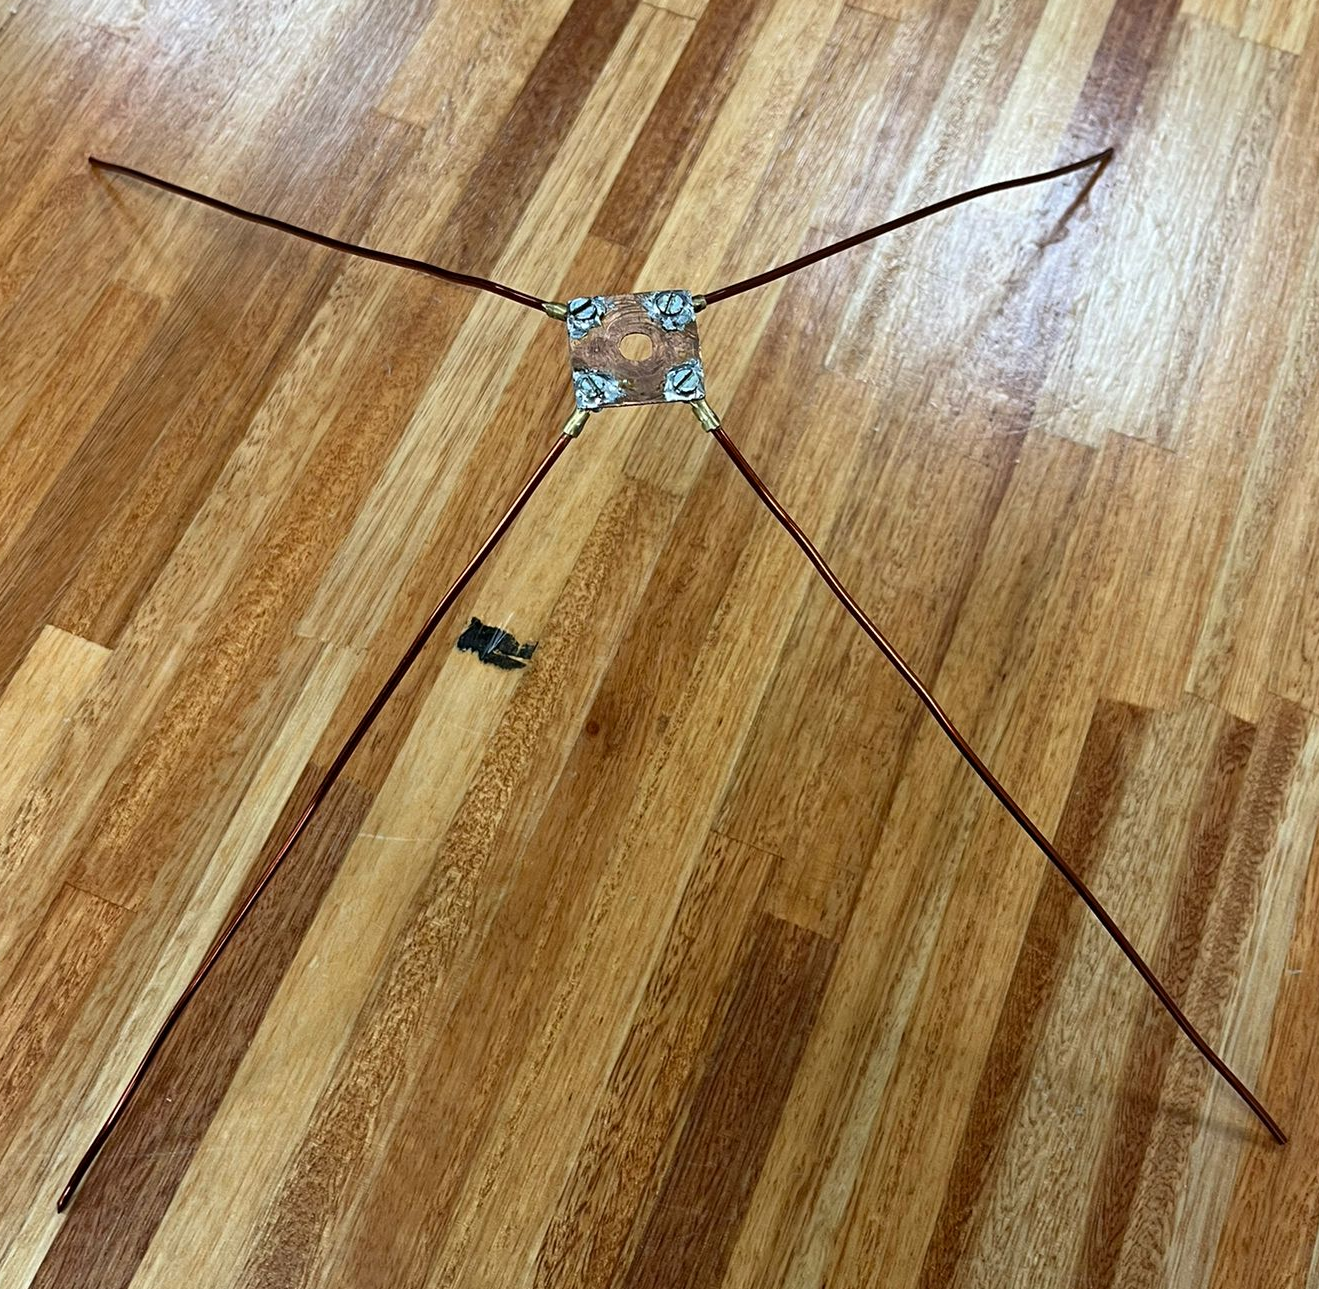
\includegraphics[width=2.0208in,keepaspectratio]{./imagenes/image61.png}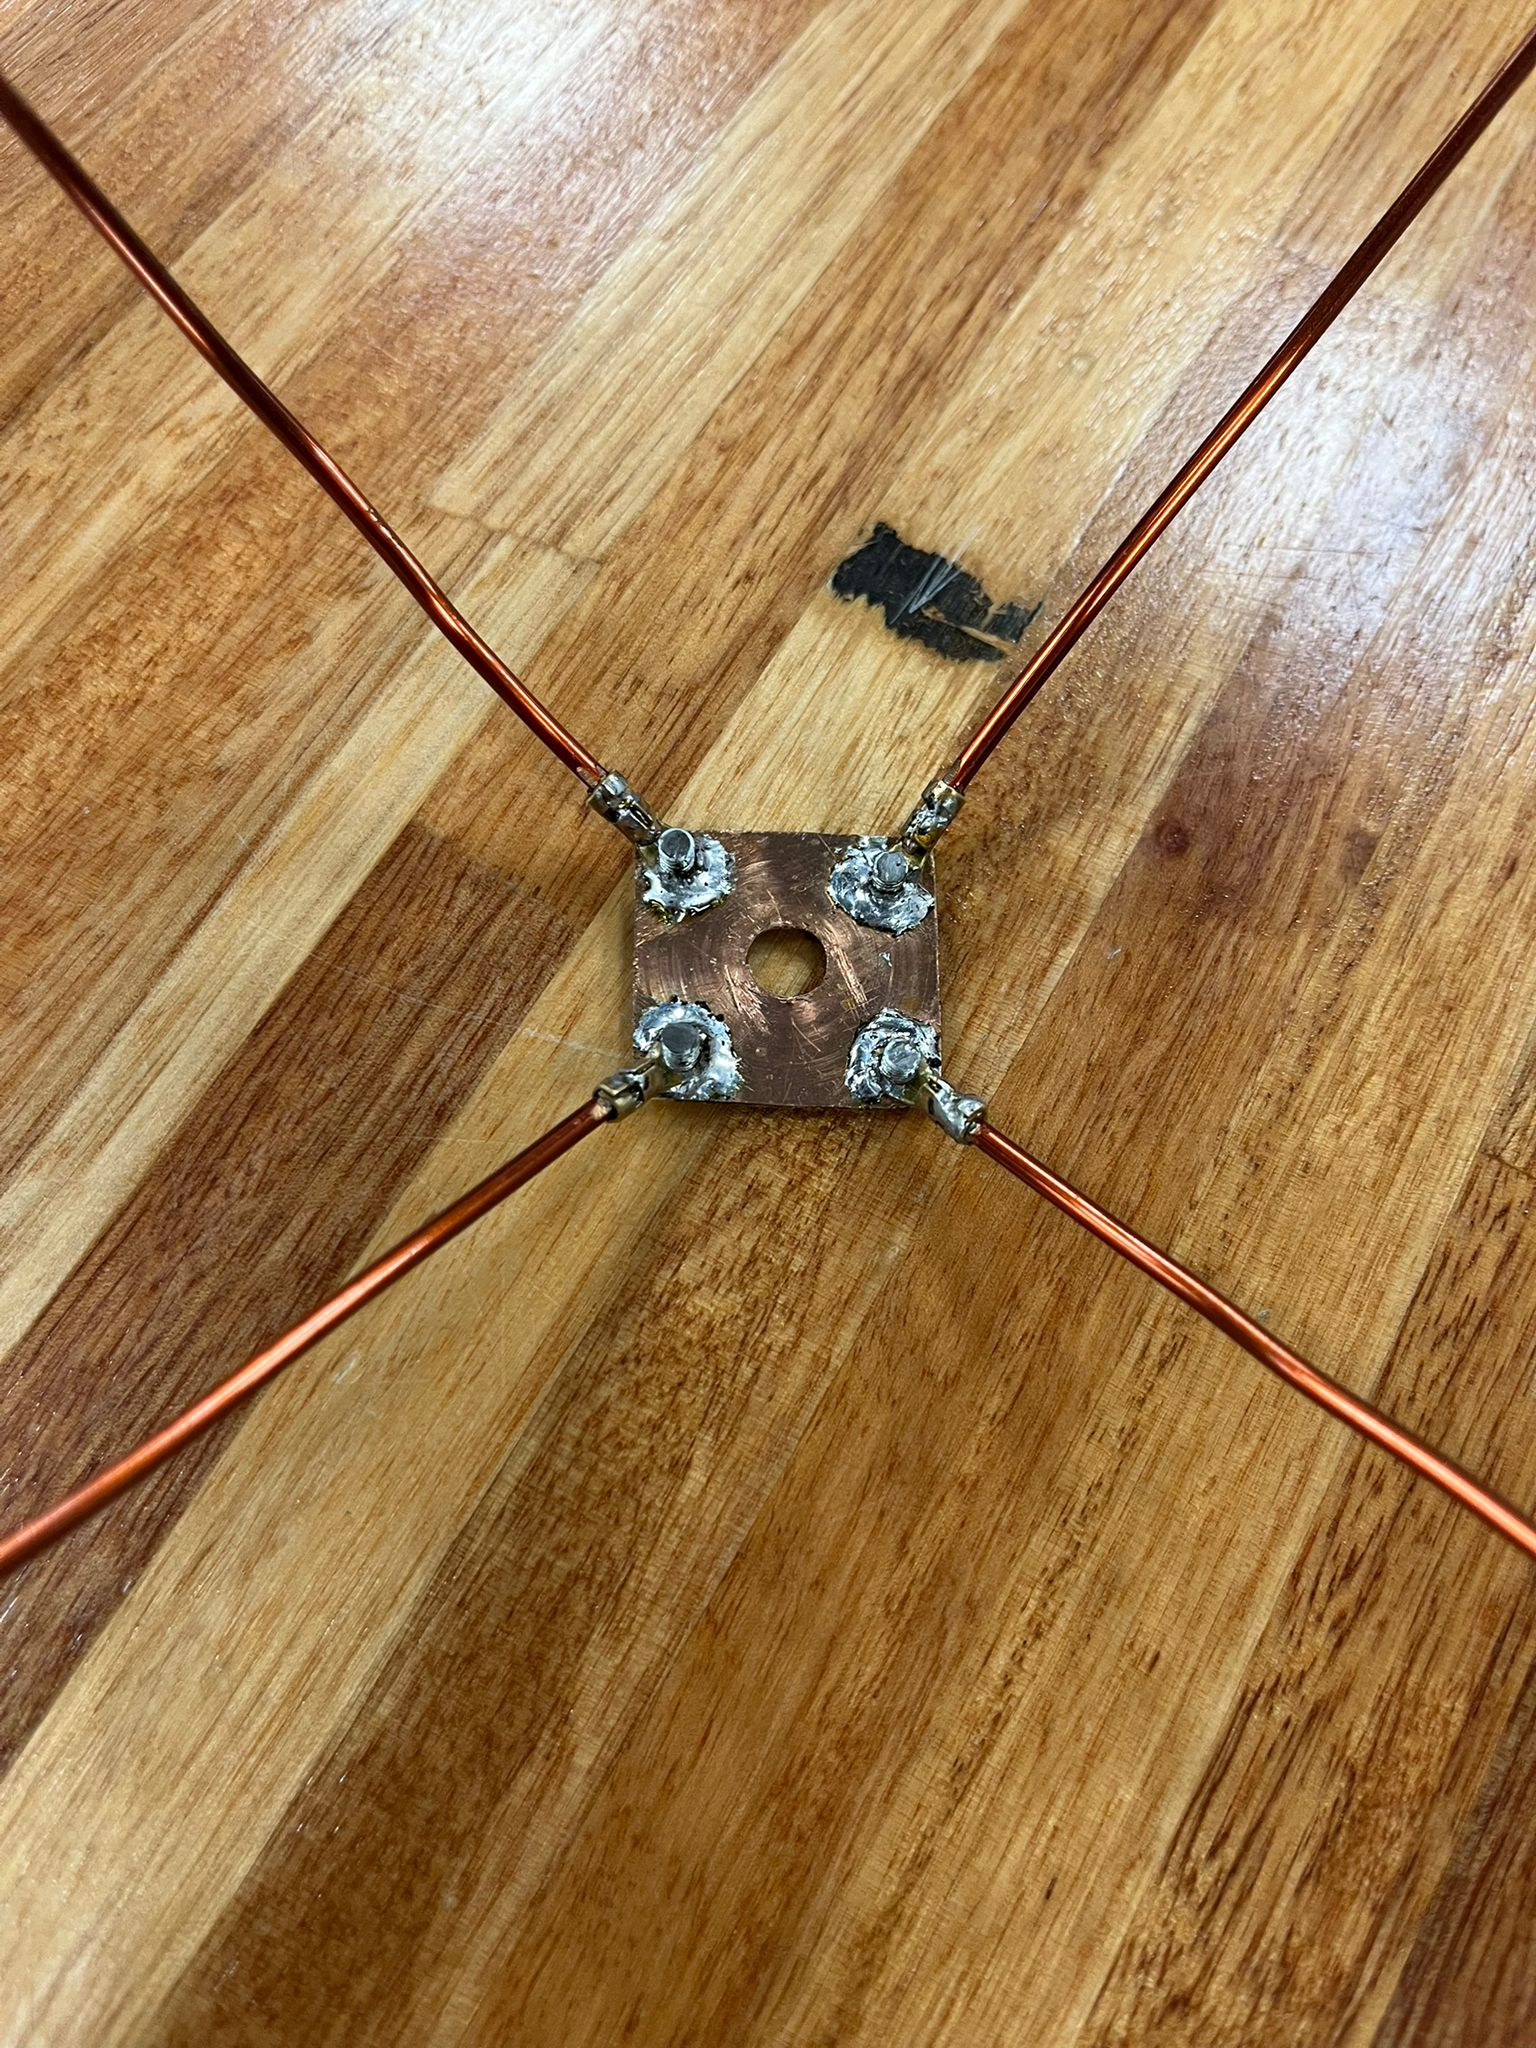
\includegraphics[width=1.4870in,keepaspectratio]{./imagenes/image83.png}

\(P_{Reflejada\ } = \ P_{Transmitida}\ .\ {(\frac{ROE\  - \ 1}{ROE\  + \ 1})}^{2}\)

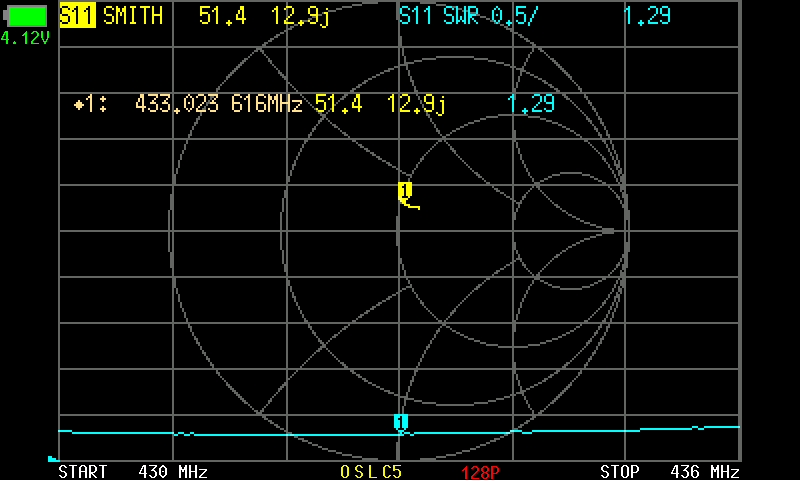
\includegraphics[width=3.5871in,keepaspectratio]{./imagenes/image41.png}

Con un SWR de 1.29 se refleja aproximadamente solo 1.62\% de la señal, lo cual indica un buen acoplamiento.

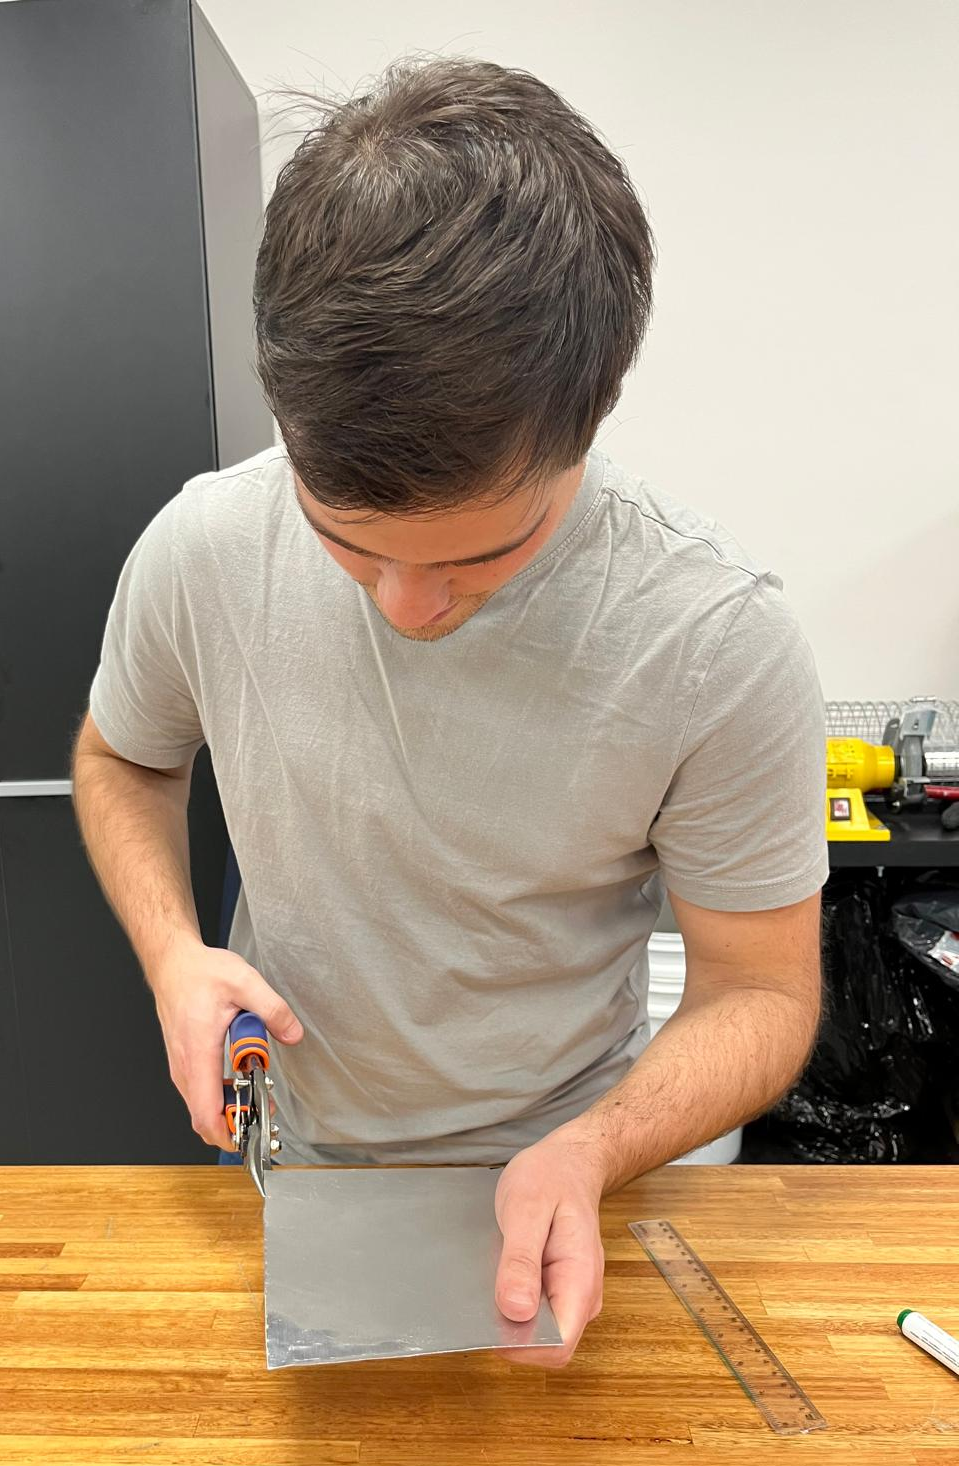
\includegraphics[width=2.2117in,keepaspectratio]{./imagenes/image29.png}

En relación a la antena de 1240 mhz, al principio se quiso construir aprovechando la cara inferior de la estructura. Para hacer el plano de tierra se cortó la base de 14x14 cm de aluminio y se realizó un orificio en el medio.

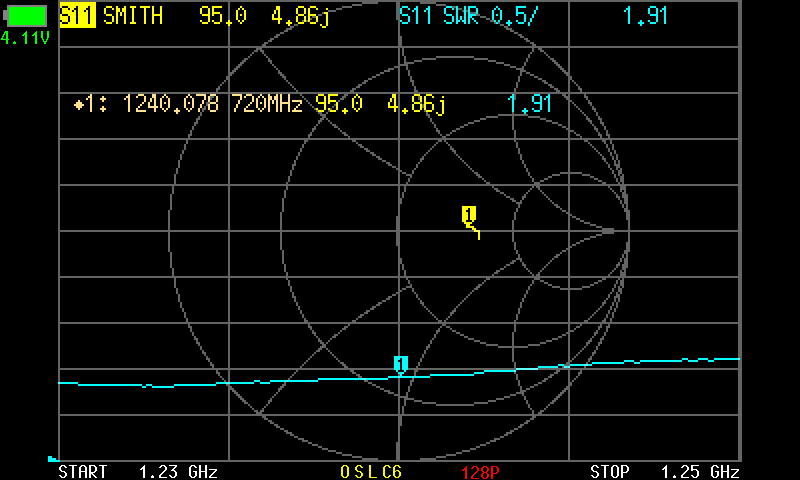
\includegraphics[width=3.4006in,keepaspectratio]{./imagenes/image64.png}

Se verificó su acoplamiento y dieron valores aceptables, pero mejorables. Con un SWR de 1.91 se refleja aproximadamente 9\% de la potencia.

Se terminó decidiendo que la antena de video se construyera con radiales debido a la flexibilidad que tiene para buscar el mejor acoplamiento posible y maximizar los valores del enlace con los recursos que se tiene.

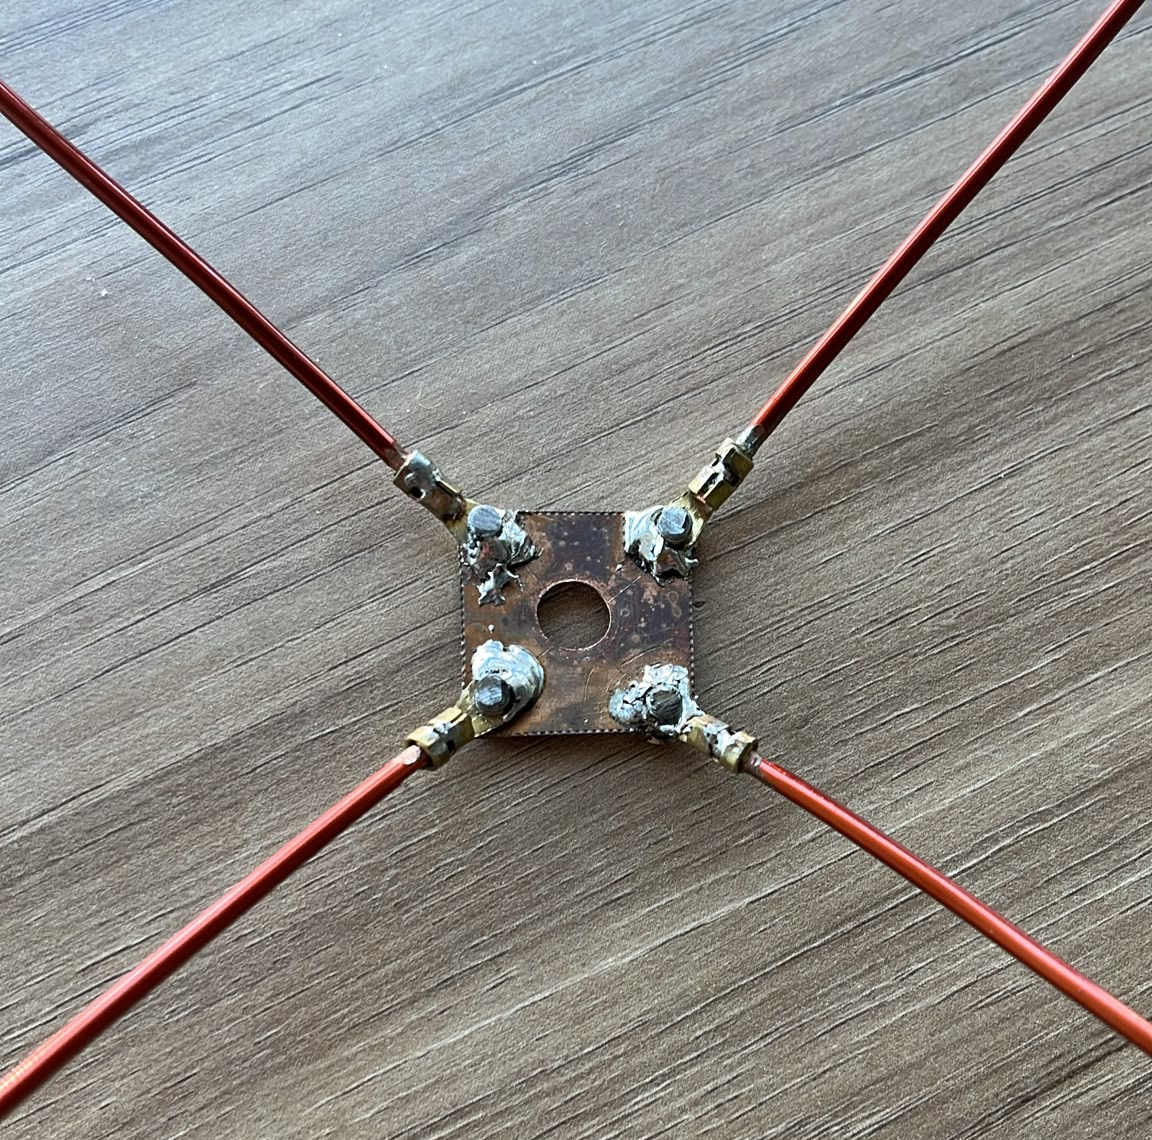
\includegraphics[width=2.2087in,keepaspectratio]{./imagenes/image22.png}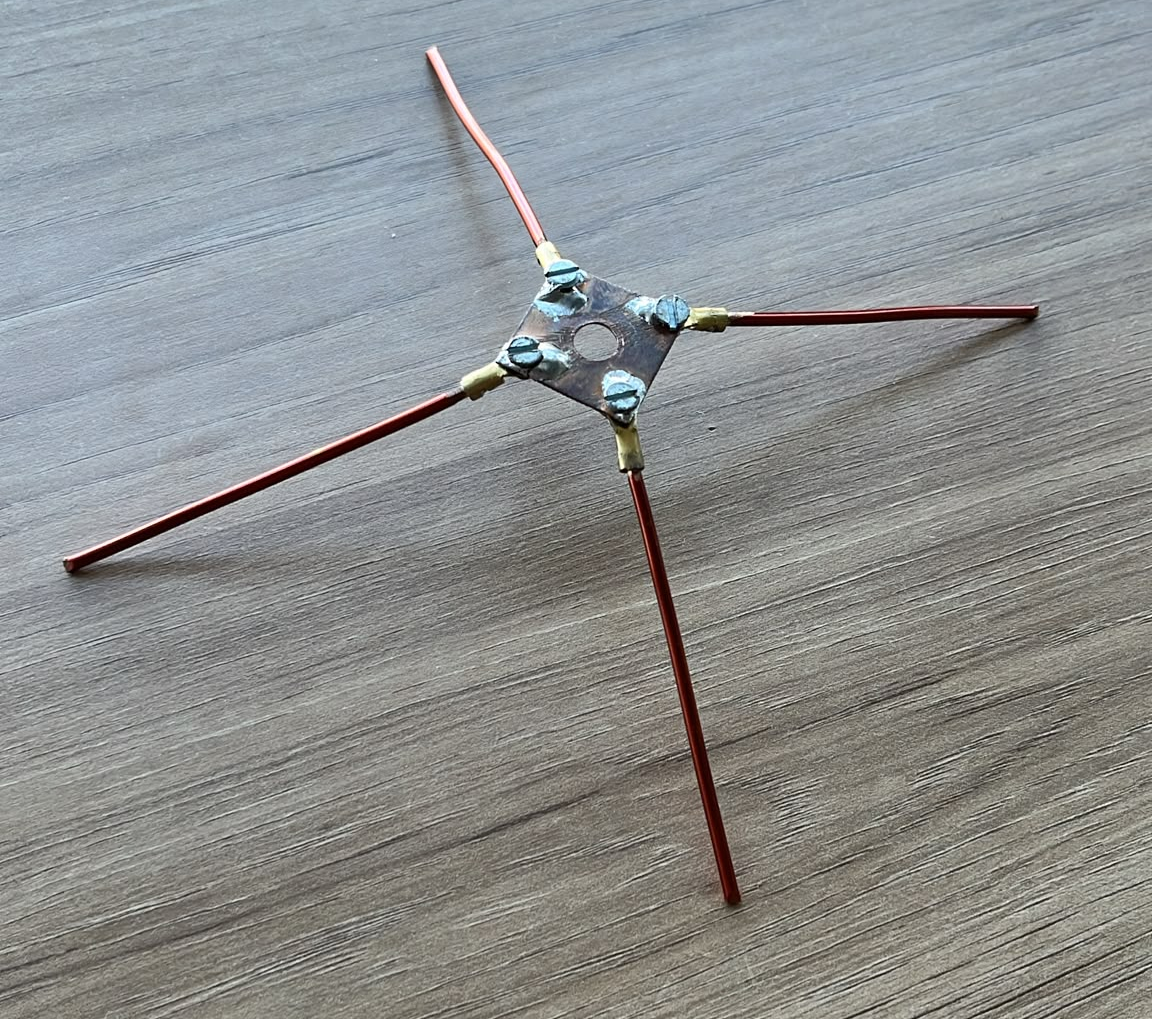
\includegraphics[width=2.4501in,keepaspectratio]{./imagenes/image28.png}

Para construir la segunda versión de la antena de video, se implementó el mismo diseño que la versión 3 de la antena de telemetría

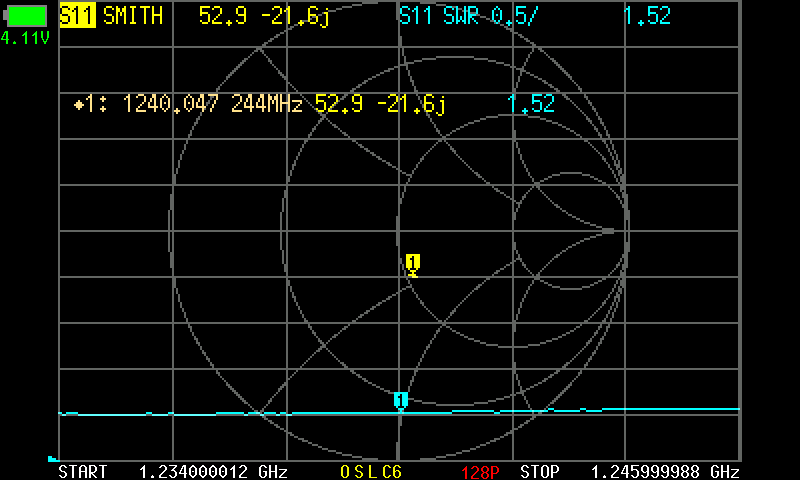
\includegraphics[width=3.6761in,keepaspectratio]{./imagenes/image6.png}

Con esta nueva versión, se logró mejorar el acoplamiento significativamente. Se pasó de tener una antena que refleja el 9\% de la potencia incidente, a tener una que solo refleja aproximadamente 3\%.

\textbf{5.2 Ubicación}

Usando la segunda versión de los radiales, se verificó el efecto que tiene la estructura metálica del payload sobre las antenas. En primer lugar se verificó la posibilidad de tener la antena de telemetría colineal a la de video.

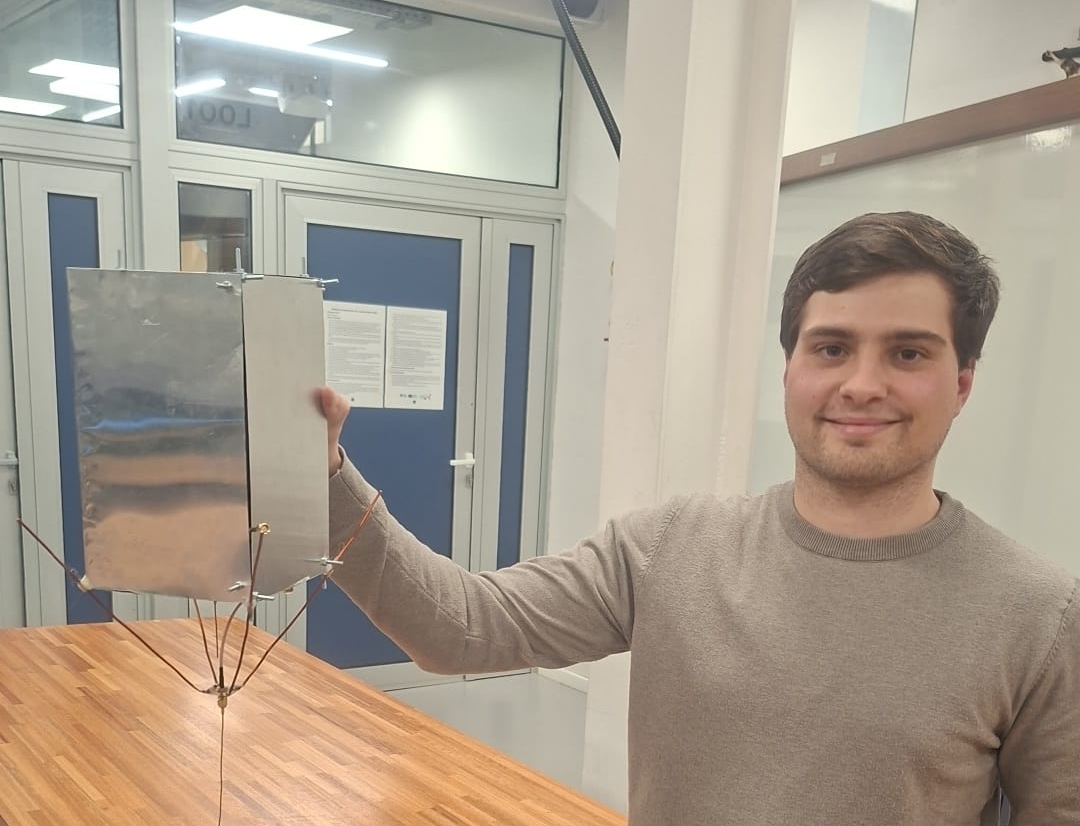
\includegraphics[width=2.4285in,keepaspectratio]{./imagenes/image48.png}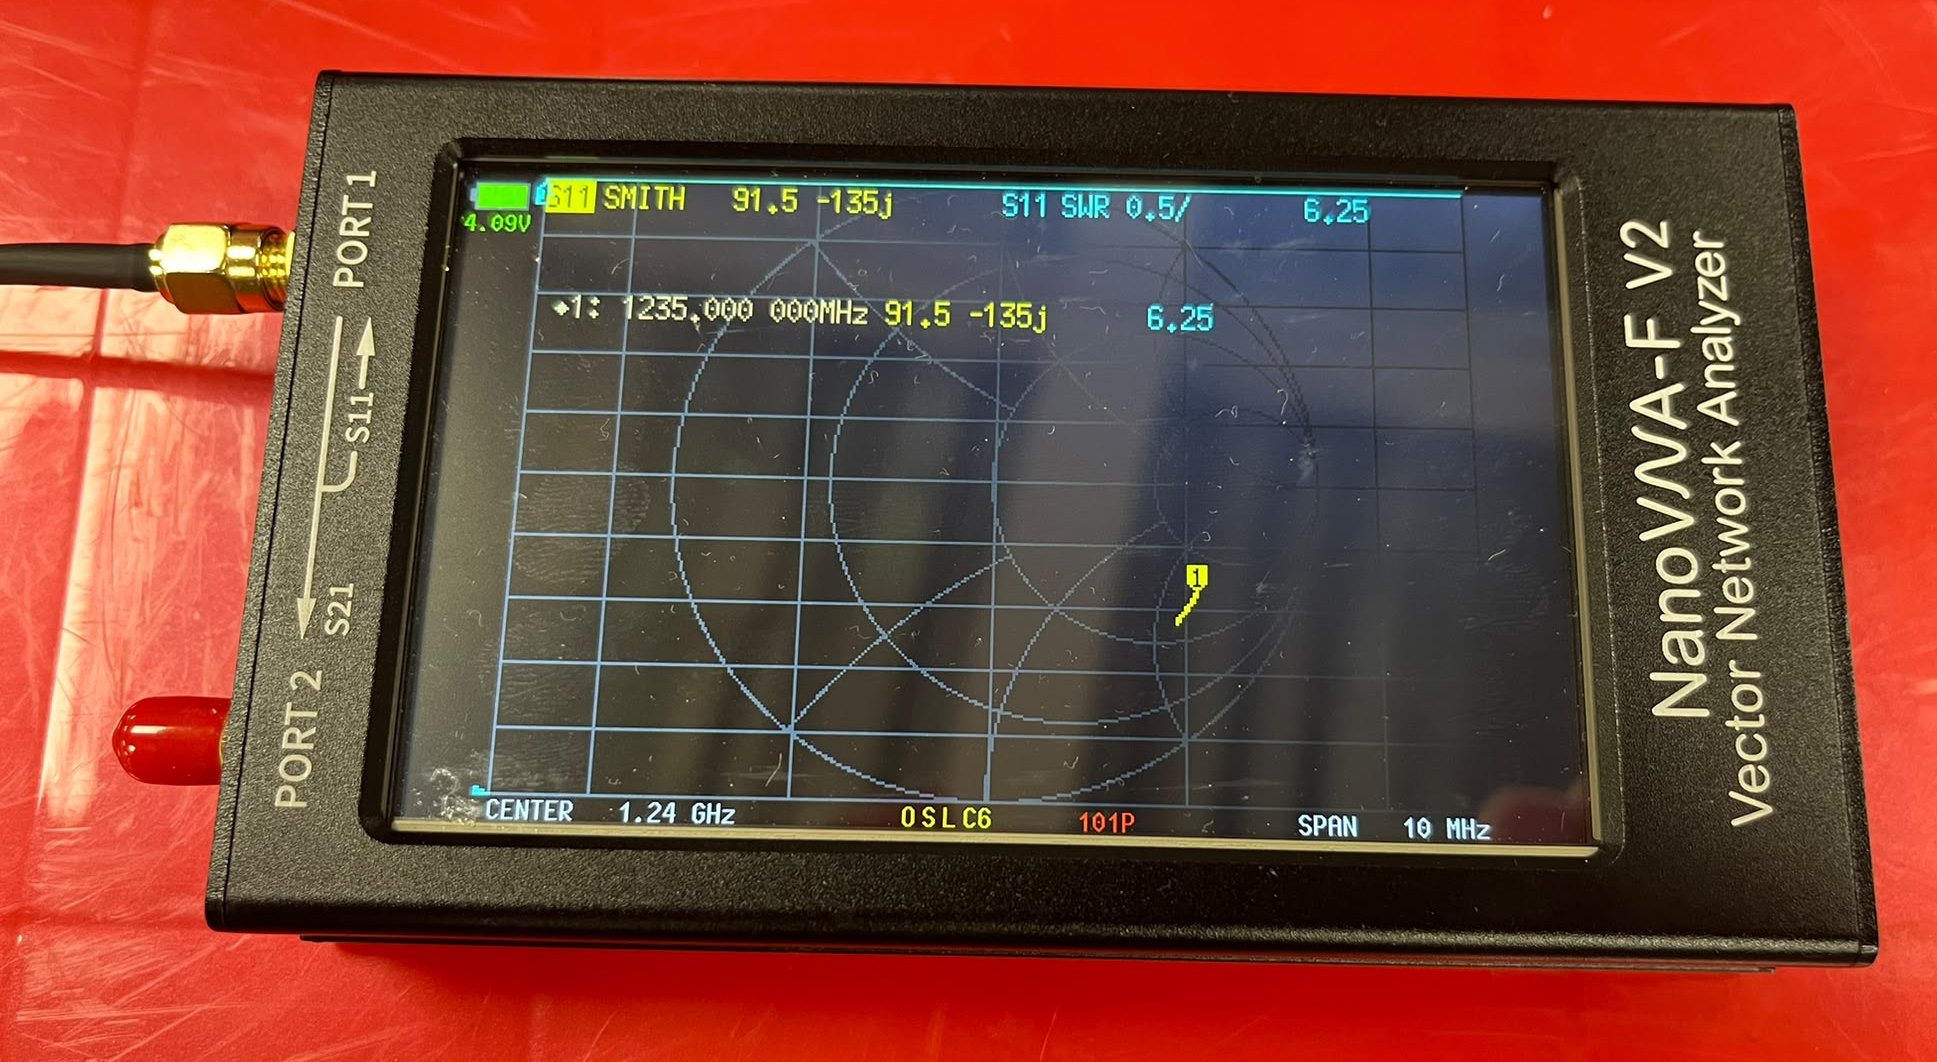
\includegraphics[width=3.3589in,keepaspectratio]{./imagenes/image91.png}

Según el resultado del VNA, tenerlas cerca, con el coaxial de telemetría pegada al radial de video afecta significativamente al acoplamiento de la antena. Con un SWR de 6.25, se refleja aproximadamente el 52\% de la potencia.

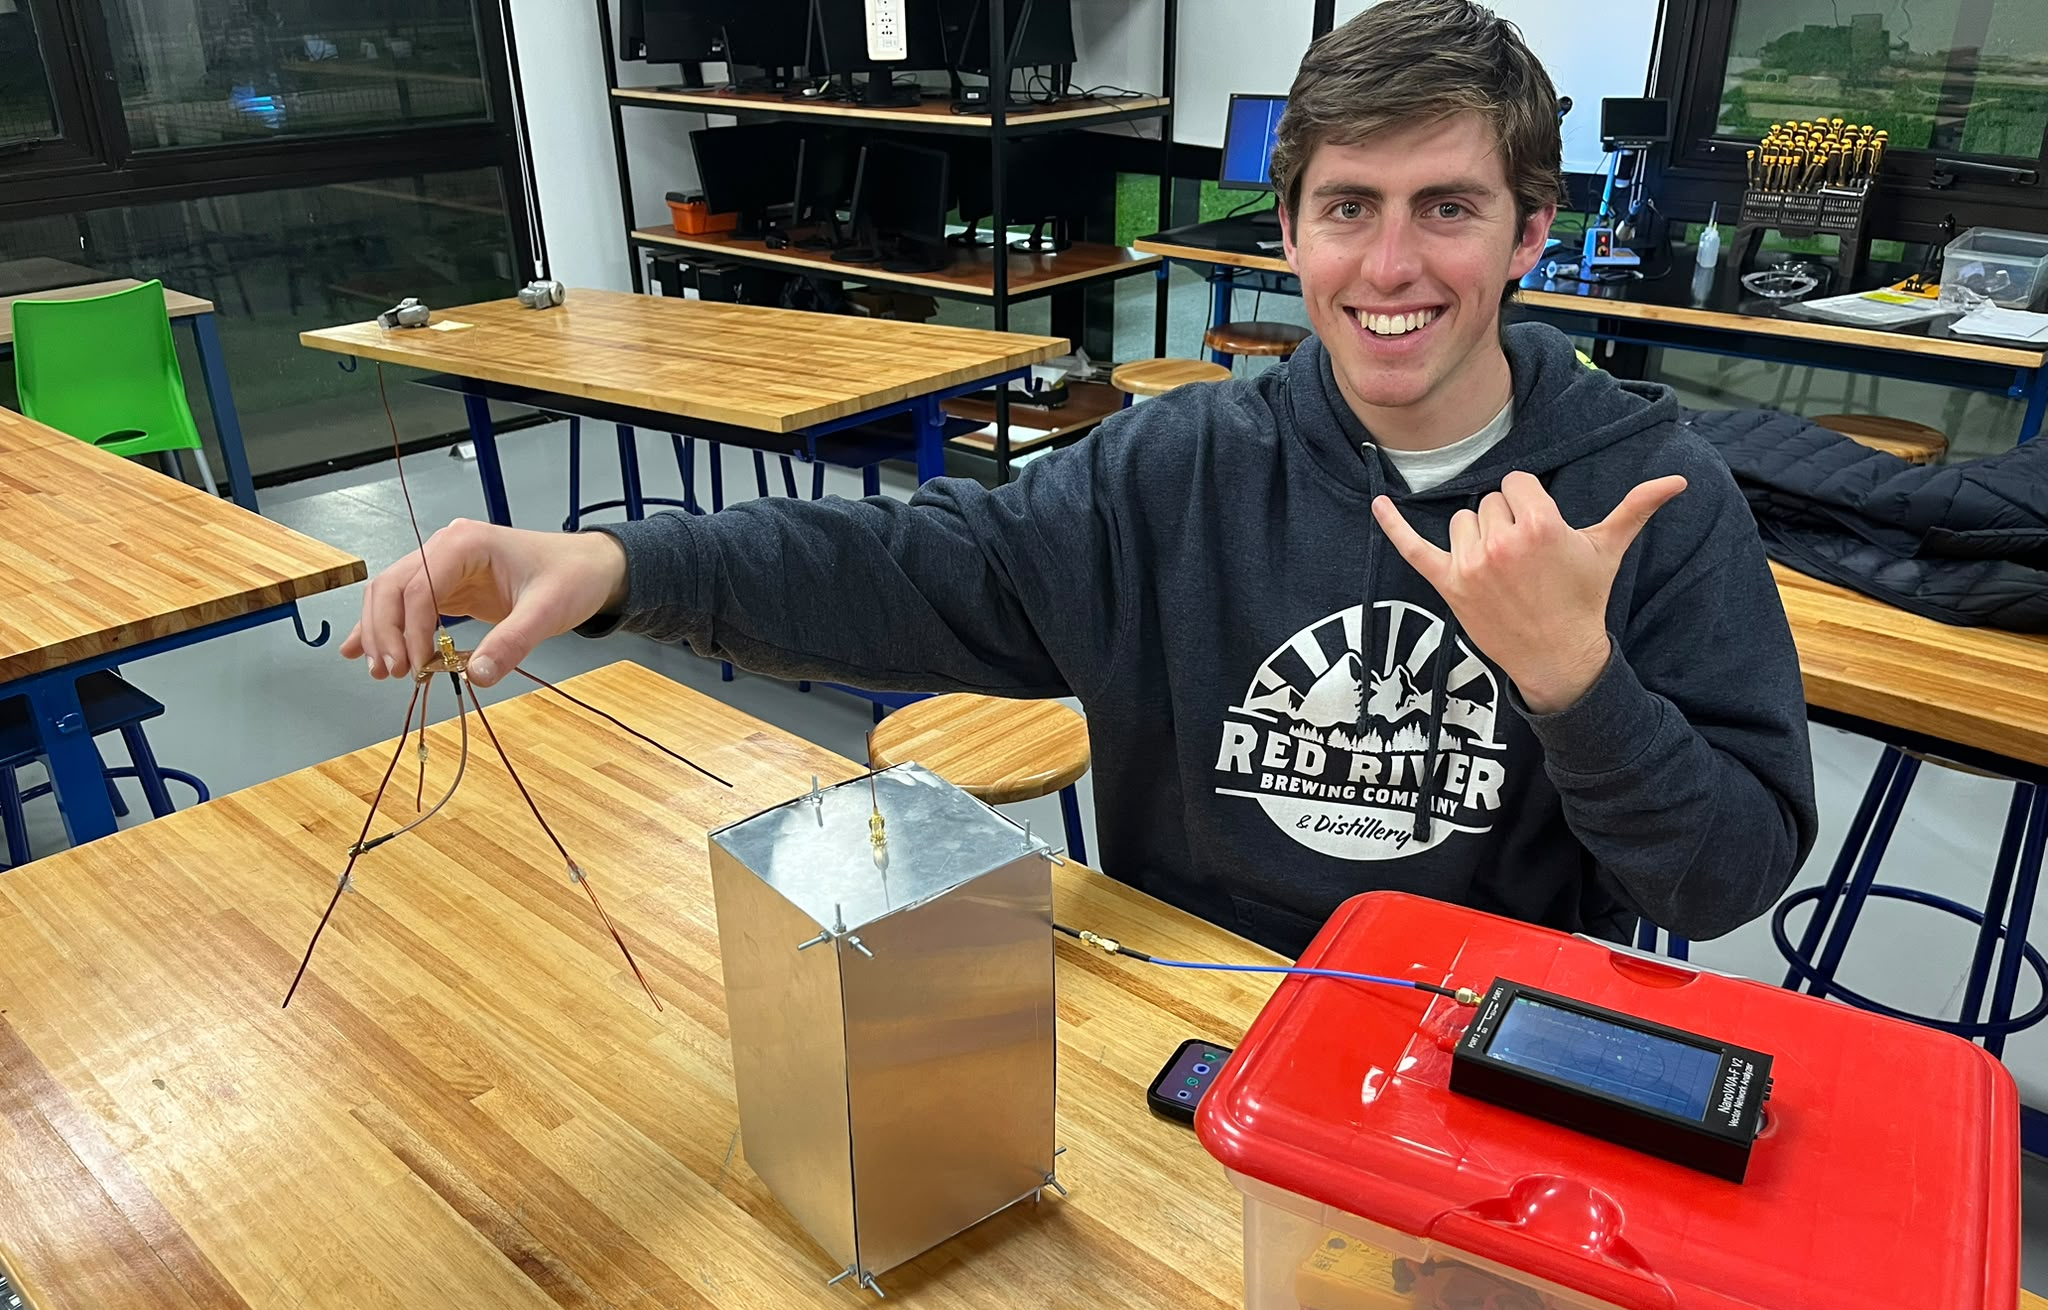
\includegraphics[width=2.6413in,keepaspectratio]{./imagenes/image30.png}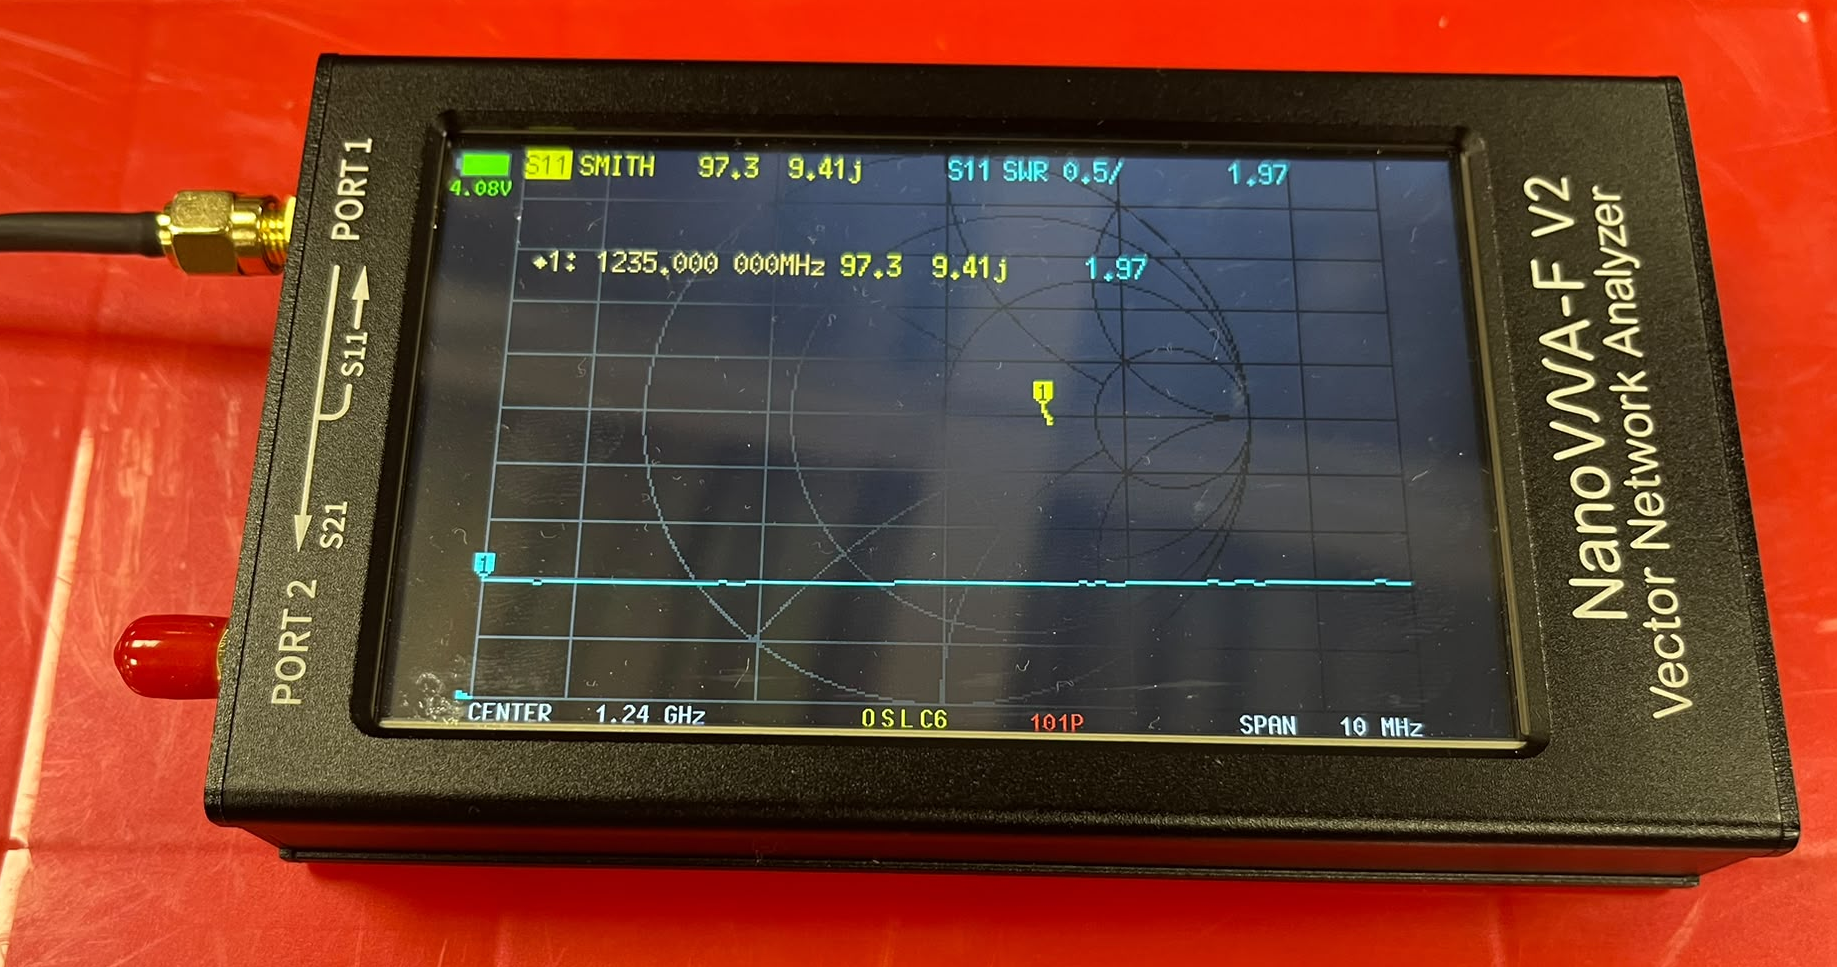
\includegraphics[width=3.1461in,keepaspectratio]{./imagenes/image69.png}

Se movió de lugar la antena de telemetría para evaluar qué otra posición puede tener para que tengan el mejor acoplamiento posible. Primero, la antena de telemetría se saco completamente y se verificó el acoplamiento de la antena de video. Se obtuvo una impedancia de 97.3 + 9.41j, generando un SWR de 1.97, el cual hace que se devuelva aproximadamente 11\% de la potencia transmitida.

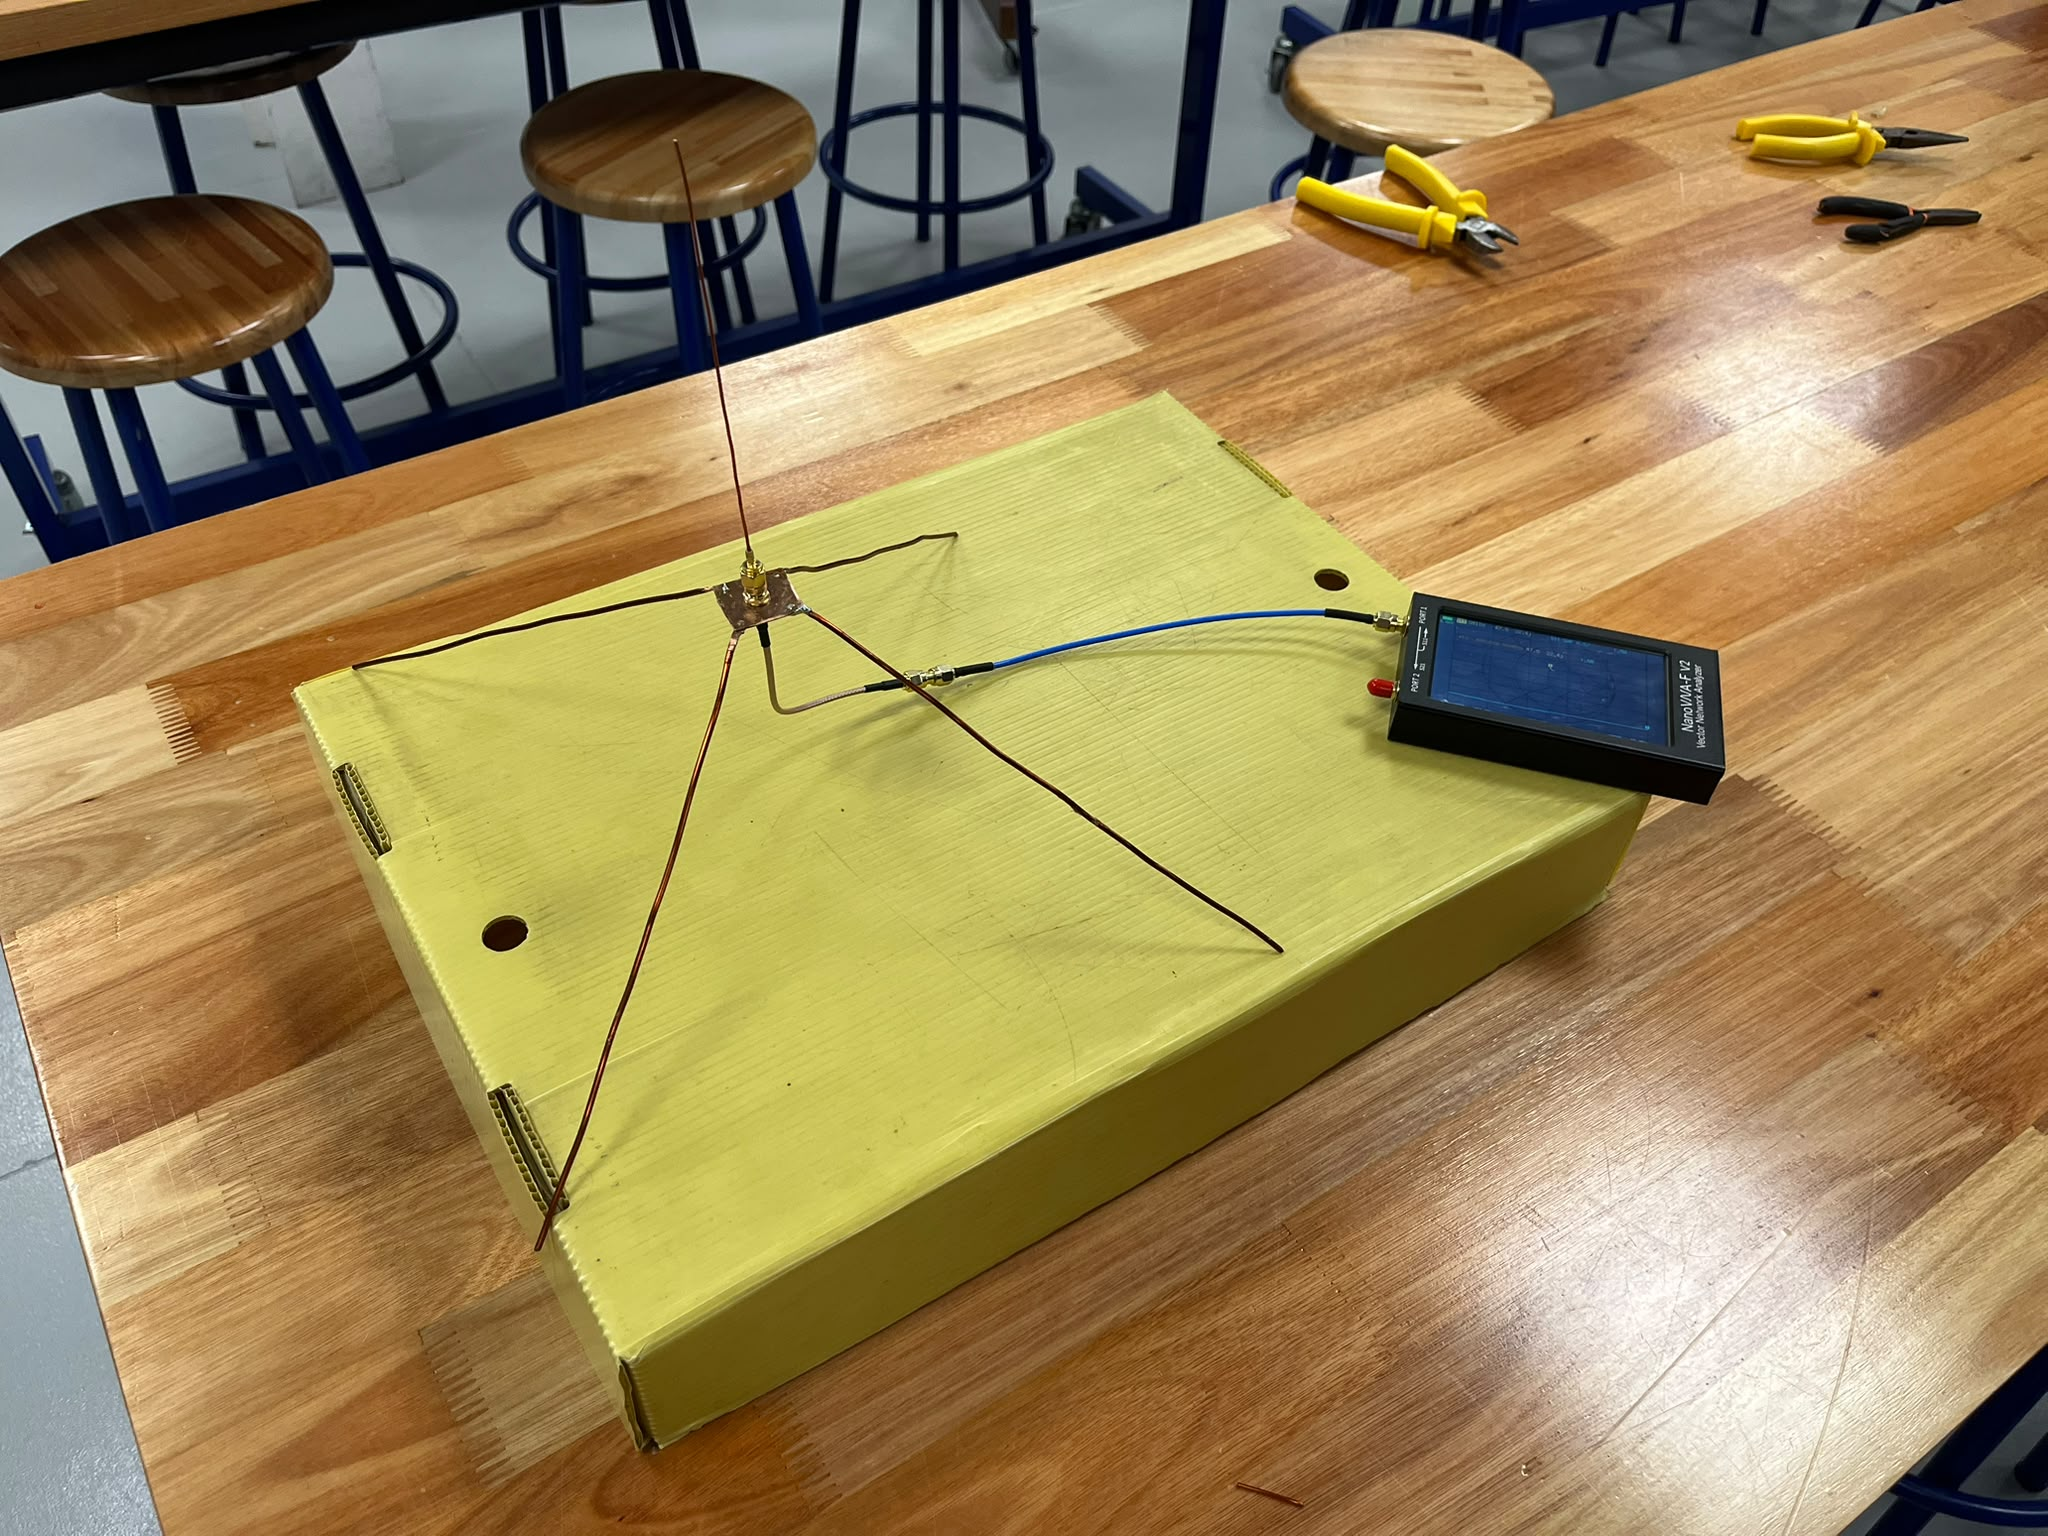
\includegraphics[width=2.4983in,keepaspectratio]{./imagenes/image16.png}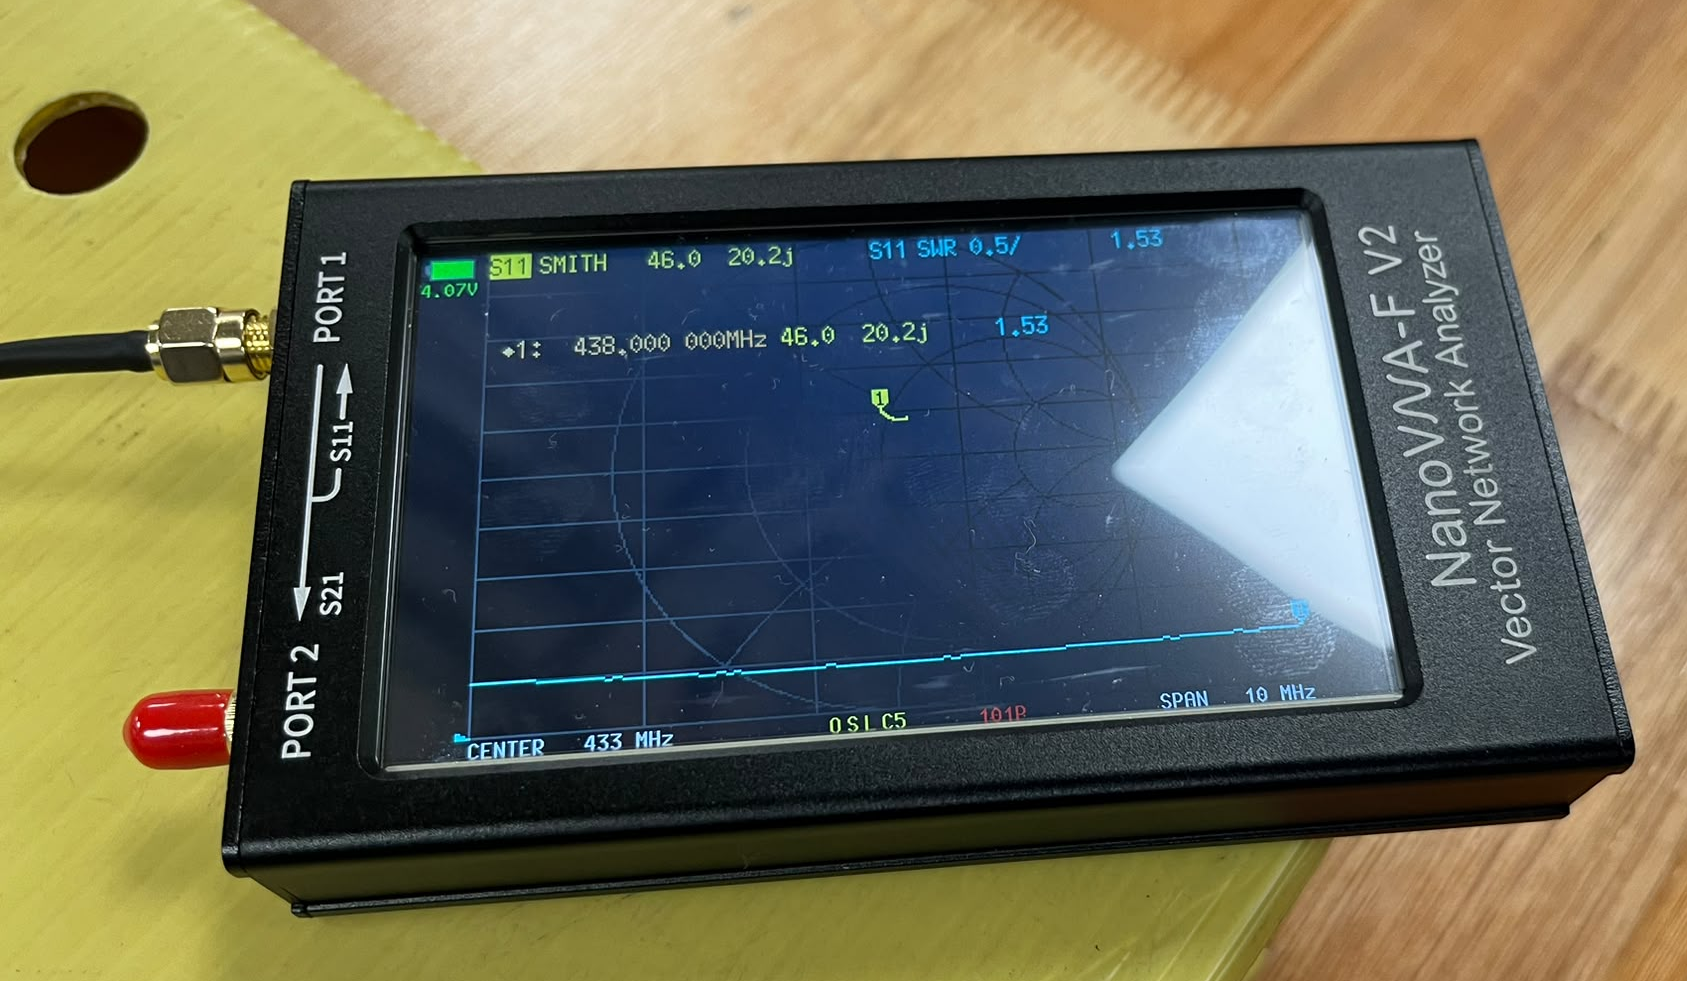
\includegraphics[width=3.2891in,keepaspectratio]{./imagenes/image13.png}

También se verificó la antena de telemetría, sin tener la estructura de aluminio cerca. Se obtuvo una impedancia de 46 + 20.2j, generando un SWR de 1.53, el cual hace que se devuelva aproximadamente 5\% de la potencia transmitida.

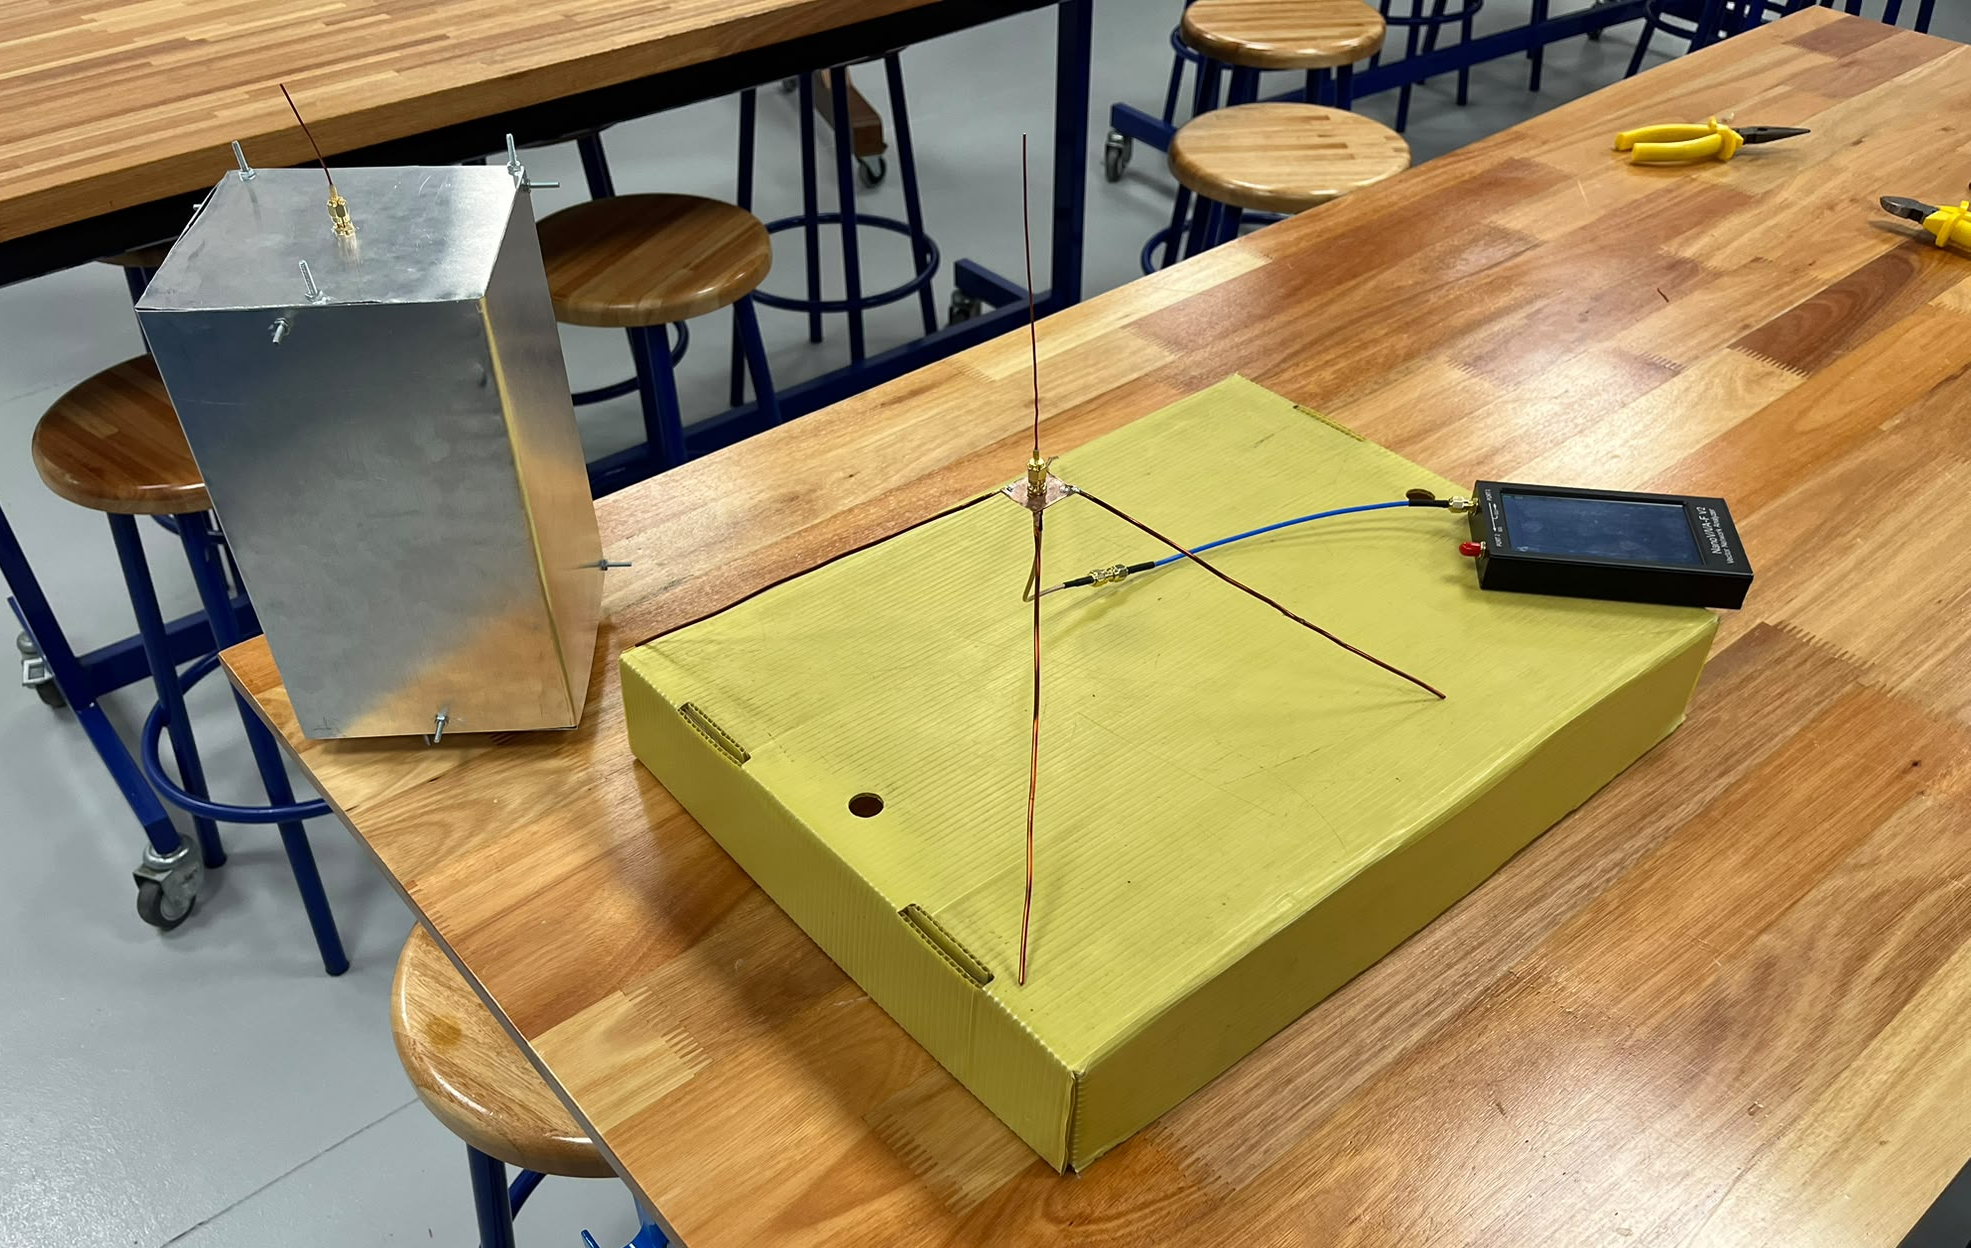
\includegraphics[width=2.5466in,keepaspectratio]{./imagenes/image47.png}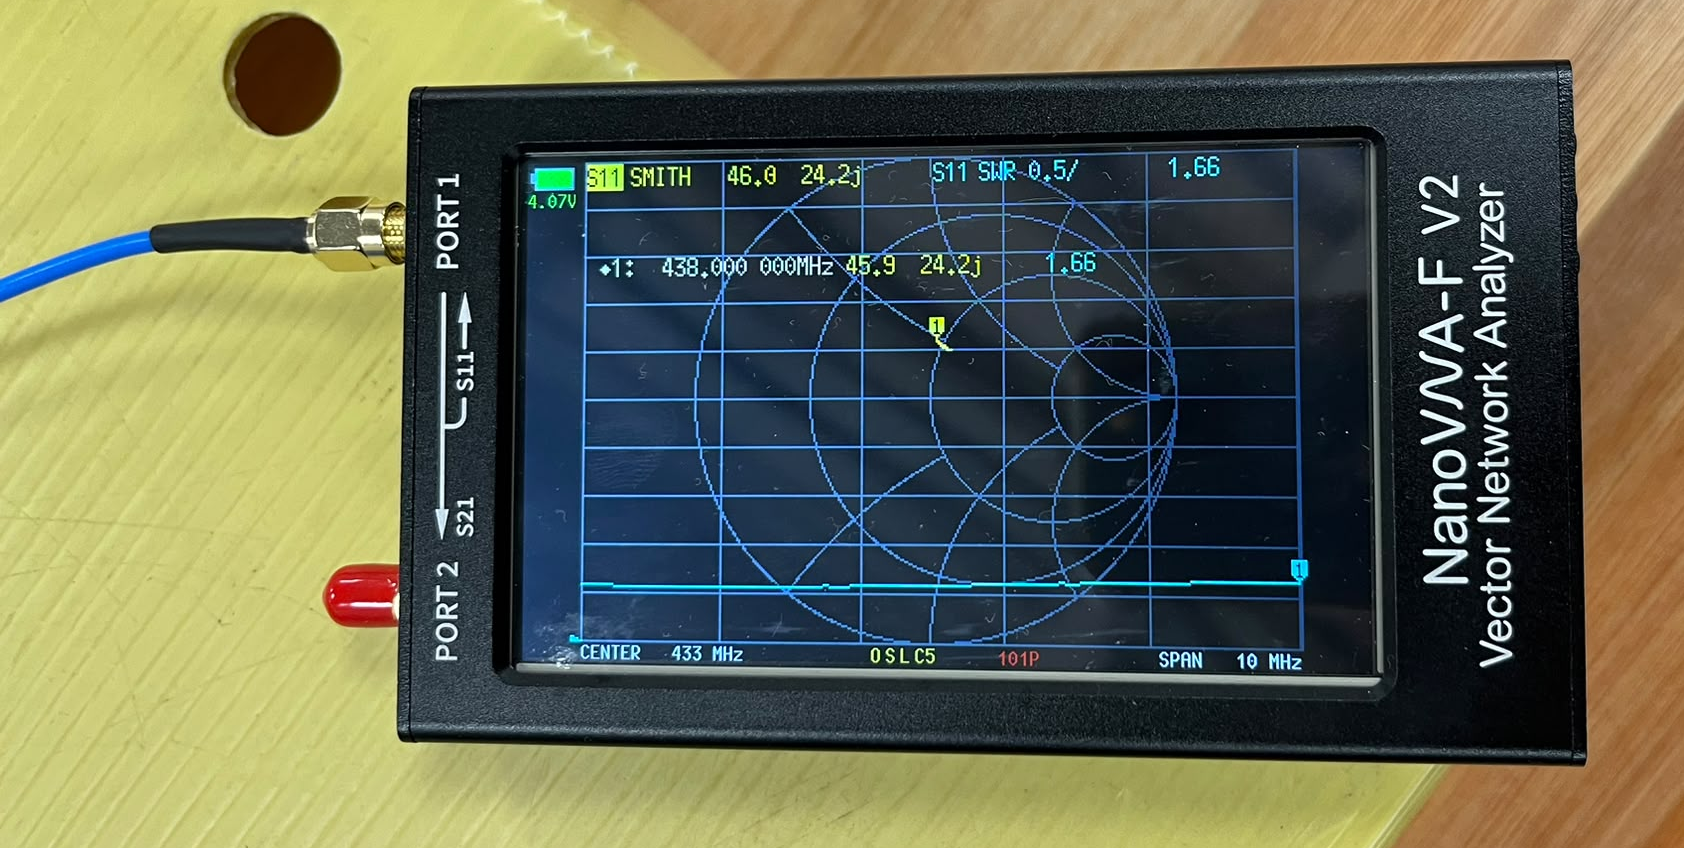
\includegraphics[width=3.2408in,keepaspectratio]{./imagenes/image71.png}

Por último, se acercó la estructura de aluminio al costado de la antena de telemetría y se verificó que el acoplamiento no empeora significativamente. Además, como las dos antenas operan en bandas diferentes, la potencia que transmite una no afecta la señal de la otra.

\section{Computadora de a bordo y software}\label{payload}

\subsection{Arquitectura de comunicación}\label{arquitectura-de-comunicaciuxf3n}

El payload está compuesto por dos placas: la placa principal y la placa de alimentación.

\textbf{Placa Principal}

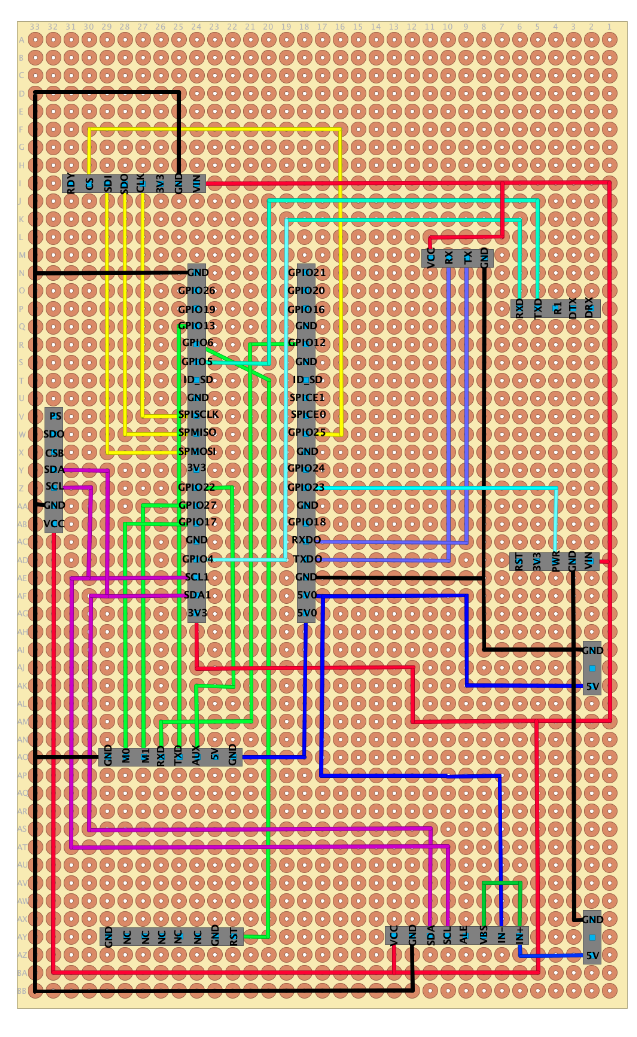
\includegraphics[width=2.1719in,keepaspectratio]{./imagenes/image94.png}

Para vincular los distintos periféricos con los pines GPIO de la placa se emplea una GPIO breakout board, lo que permite distribuir de forma ordenada las conexiones hacia los diferentes módulos. Las componentes conectados a la placa principal junto a su funcion y el detalle de conexiones se encuentran a continuacion.

\subsubsection*{U-Blox NEO-6M}\phantomsection\label{u-blox-neo-6m}

El módulo GPS U-Blox NEO-6M se encarga de recibir las coordenadas de posición del payload durante el vuelo. Se comunica con la Raspberry Pi mediante el protocolo UART0, disponible en los pines GPIO 14 y 15 (RXD0/TXD0).

{\def\LTcaptype{none} % do not increment counter
\begin{longtable}[]{@{}
  >{\centering\arraybackslash}p{(\linewidth - 4\tabcolsep) * \real{0.1815}}
  >{\centering\arraybackslash}p{(\linewidth - 4\tabcolsep) * \real{0.3051}}
  >{\centering\arraybackslash}p{(\linewidth - 4\tabcolsep) * \real{0.1510}}@{}}
\toprule\noalign{}
\endhead
\bottomrule\noalign{}
\endlastfoot
\textbf{Pin módulo} & \textbf{Conexión Raspberry Pi} & \textbf{Función} \\
VCC & 3V3 & Alimentación \\
GND & GND & Alimentación \\
RX & UART0 TX Raspberry Pi & Datos \\
TX & UART0 RX Raspberry Pi & Datos \\
\end{longtable}
}

\textbf{BC660K-GL}

El módulo BC660K-GL provee conectividad Narrowband IoT (NB-IoT), utilizada como enlace para la transmisión de datos del payload. La comunicación con la Raspberry Pi se realiza mediante UART3, habilitado en los pines GPIO 4 y 5.

{\def\LTcaptype{none} % do not increment counter
\begin{longtable}[]{@{}
  >{\centering\arraybackslash}p{(\linewidth - 4\tabcolsep) * \real{0.1670}}
  >{\centering\arraybackslash}p{(\linewidth - 4\tabcolsep) * \real{0.3196}}
  >{\centering\arraybackslash}p{(\linewidth - 4\tabcolsep) * \real{0.1606}}@{}}
\toprule\noalign{}
\endhead
\bottomrule\noalign{}
\endlastfoot
\textbf{Pin módulo} & \textbf{Conexión Raspberry Pi} & \textbf{Función} \\
TX / RX & UART3 (GPIO 4/5) & Datos \\
VIN & 3V3 & Alimentación \\
GND & GND & Alimentación \\
PWR & GPIO 23 (salida) & \\
\end{longtable}
}

\textbf{EBYTE LoRa E22-400T22S}

El módulo EBYTE LoRa E22-400T22S es el encargado de transmitir la telemetría del payload durante el vuelo. Se comunica con la Raspberry Pi a través de UART5, en los pines GPIO 12 y 13.

{\def\LTcaptype{none} % do not increment counter
\begin{longtable}[]{@{}
  >{\centering\arraybackslash}p{(\linewidth - 4\tabcolsep) * \real{0.1751}}
  >{\centering\arraybackslash}p{(\linewidth - 4\tabcolsep) * \real{0.3164}}
  >{\centering\arraybackslash}p{(\linewidth - 4\tabcolsep) * \real{0.3935}}@{}}
\toprule\noalign{}
\endhead
\bottomrule\noalign{}
\endlastfoot
\textbf{Pin módulo} & \textbf{Conexión Raspberry Pi} & \textbf{Función} \\
M0 & GPIO 17 (salida) & Configuración de modo \\
M1 & GPIO 27 (salida) & Configuración de modo \\
RXD & UART5 TX Raspberry Pi & Datos \\
TXD & UART5 RX Raspberry Pi & Datos \\
AUX & GPIO 22 (entrada) & Indica si el módulo está ocupado \\
5V & 5V & Alimentación \\
GND & GND & Alimentación \\
RST & GPIO 6 (salida) & Reset \\
\end{longtable}
}

\textbf{MS5611}

El sensor MS5611 mide presión y temperatura, y se utiliza específicamente para monitorear la temperatura interna del payload. Se comunica mediante el protocolo I2C, sobre el bus compartido I2C1 de la Raspberry Pi, en la dirección 0x77.

{\def\LTcaptype{none} % do not increment counter
\begin{longtable}[]{@{}
  >{\centering\arraybackslash}p{(\linewidth - 4\tabcolsep) * \real{0.1654}}
  >{\centering\arraybackslash}p{(\linewidth - 4\tabcolsep) * \real{0.3373}}
  >{\centering\arraybackslash}p{(\linewidth - 4\tabcolsep) * \real{0.2168}}@{}}
\toprule\noalign{}
\endhead
\bottomrule\noalign{}
\endlastfoot
\textbf{Pin módulo} & \textbf{Conexión Raspberry Pi} & \textbf{Función} \\
VCC & 3V3 & Alimentación \\
GND & GND & Alimentación \\
SDA & SDA1 (bus I2C compartido) & Datos \\
SCL & SCL1 (bus I2C compartido) & Clock \\
\end{longtable}
}

\textbf{INA226}

El sensor INA226 mide el consumo total de corriente del payload. Se instala en serie entre la placa de energía, compuesta por las baterías y el stepdown, y la Raspberry Pi, y se comunica mediante el mismo bus I2C1 compartido, en la dirección 0x40.

{\def\LTcaptype{none} % do not increment counter
\begin{longtable}[]{@{}
  >{\centering\arraybackslash}p{(\linewidth - 4\tabcolsep) * \real{0.2083}}
  >{\centering\arraybackslash}p{(\linewidth - 4\tabcolsep) * \real{0.3100}}
  >{\centering\arraybackslash}p{(\linewidth - 4\tabcolsep) * \real{0.4817}}@{}}
\toprule\noalign{}
\endhead
\bottomrule\noalign{}
\endlastfoot
\textbf{Pin módulo} & \textbf{Conexión} & \textbf{Función} \\
IN+ & Salida del stepdown (5V) & Entrada de corriente \\
IN− & 5V de la Raspberry Pi & Salida de corriente hacia la Raspberry Pi \\
VBS & Puenteado a IN+ & Lectura de voltaje \\
SDA & SDA1 (bus I2C compartido) & Datos \\
SCL & SCL1 (bus I2C compartido) & Clock \\
VCC & 3V3 & Alimentación \\
GND & GND & Alimentación \\
\end{longtable}
}

\textbf{MAX31865}

El sensor MAX31865 mide temperatura y se comunica con la Raspberry Pi mediante el protocolo SPI, utilizando los pines SPI\_CLK, SPI\_MOSI y SPI\_MISO.

{\def\LTcaptype{none} % do not increment counter
\begin{longtable}[]{@{}
  >{\centering\arraybackslash}p{(\linewidth - 4\tabcolsep) * \real{0.2216}}
  >{\centering\arraybackslash}p{(\linewidth - 4\tabcolsep) * \real{0.2794}}
  >{\centering\arraybackslash}p{(\linewidth - 4\tabcolsep) * \real{0.2971}}@{}}
\toprule\noalign{}
\endhead
\bottomrule\noalign{}
\endlastfoot
\textbf{Pin módulo} & \textbf{Conexión Raspberry Pi} & \textbf{Función} \\
CS & GPIO 25 (salida) & Chip select SPI \\
SDI / SDO / CLK & Bus SPI & Datos y clock \\
VCC & 3V3 & Alimentación \\
GND & GND & Alimentación \\
\end{longtable}
}

\textbf{Terminales Borne}

La placa cuenta con dos terminales borne que conectan la placa de alimentación con el resto del sistema.

\begin{itemize}
\item
  \textbf{Borne 1:} conecta al IN+ y al GND de la Raspberry Pi.
\item
  \textbf{Borne 2:} conectado al IN− y al GND del Borne 1.
\end{itemize}

\textbf{Otras conexiones}

Además de los módulos anteriores, el payload incorpora un Pluto SDR, utilizado como radio para la transmisión de video. Este dispositivo se conecta a la Raspberry Pi mediante USB. La Raspberry Pi Camera se conecta por el puerto CSI, sin usar pines GPIO del header.

\subsection{Configuración Raspberry Pi}\label{configuraciuxf3n-raspberry-pi}

Para habilitar el uso de las interfaces UART, SPI e I2C se debe cambiar el archivo de configuración de la Raspi ``/boot/firmware/config.txt''.

dtparam=i2c\_arm=on

dtparam=spi=on

dtparam=uart0=on

\subsection{Arquitectura de software}\label{arquitectura-de-software}

El firmware engloba los subsistemas de adquisición de telemetría, transmisión de telemetría a la estación terrena, transmisión de video a la estación terrena, control del mecanismo de liberación de globo (paracaídas/corte), lógica de modos de operación, almacenamiento local de telemetría, información de vuelo y video, y gestión de energía y batería. Todo esto siendo lo más tolerante a fallos posible.

\subsubsection{Esquema General}\label{esquema-general}

El software de payload corre en Python 3 y se ejecuta como un único proceso en la Raspberry Pi. Al arrancar crea una sesión de almacenamiento, inicializa los sensores y los transmisores, y lanza distintos hilos de la clase Thread de la librería threading que corren en paralelo dentro del proceso.

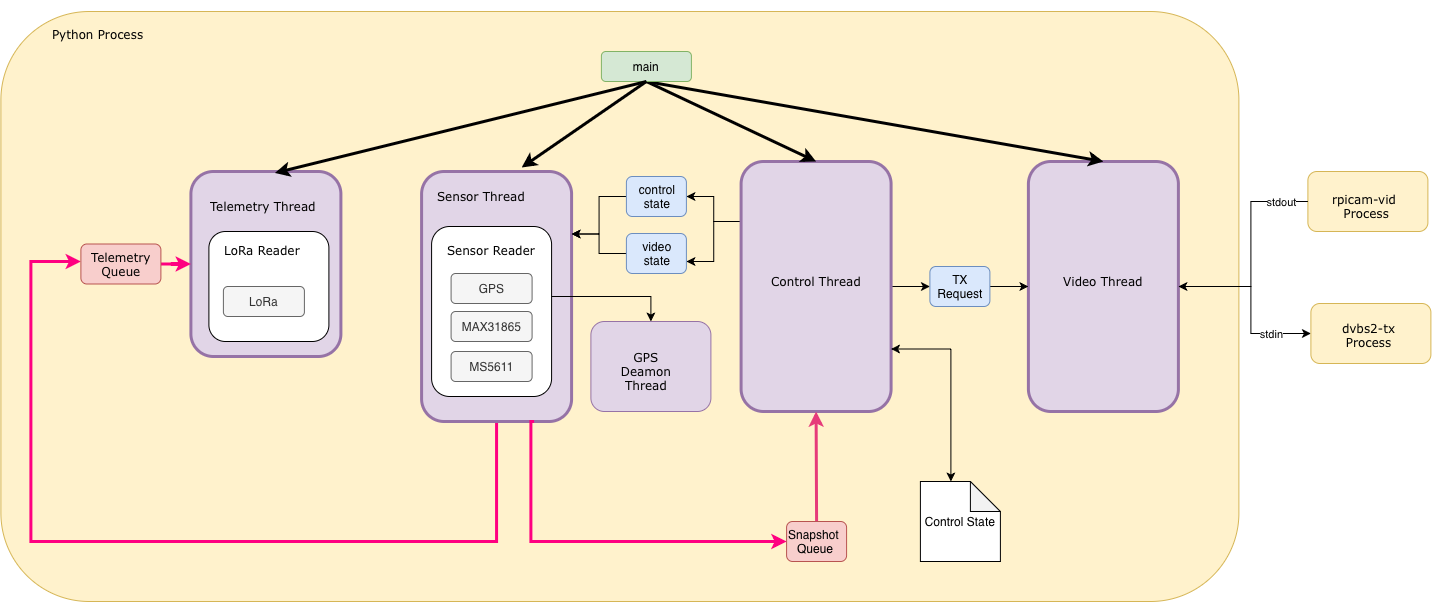
\includegraphics[width=\linewidth,keepaspectratio]{./imagenes/image9.png}

Dentro del programa principal se manejan cuatro hilos de trabajo:

\begin{itemize}
\item
  Sensor Thread
\item
  Telemetry Thread
\item
  Video Thread
\item
  Control Thread
\end{itemize}

Dichos hilos se comunican a través de colas y de variables. La colas de la libreria queue son de tamaño 1, a lo que un nuevo elemento en la cola sobrescribe al que ya existe. Las dos Colas de la clase Queue de la librería queue implementadas son:

\begin{itemize}
\item
  Cola de Paquete: Sensor Thread lee los datos de los sensores y los deja disponibles para que Telemetry Thread los consuma.
\item
  Cola de Estado: Sensor Thread pública la altitud, latitud y la longitud del payload para que el Control Thread tome las decisiones de vuelo.
\end{itemize}

Variables compartidas:

\begin{itemize}
\item
  Control Thread es dueño de las variables que guardan el estado actual del payload (fase de vuelo o si se está transmitiendo video). Esta variable la lee Sensor Thread para incluirla en el paquete que luego se envía a la Estación Terrena. Se implementa con mecanismo de Lock para evitar que Sensor Thread lea el valor mientras Control Thread lo está actualizando, lo que podría dar una lectura inconsistente o a medio escribir.
\item
  Control Thread modifica el flag que indica que se debe transmitir video. Esta se lee por Video Thread, que comienza o detiene la transmisión de video.
\end{itemize}

Además, un hilo auxiliar de GPS, lanzado por el Sensor Thread, lee las tramas NMEA por UART en background y guarda la última posición válida calculada por el receptor (fix), de forma que el Sensor Thread pueda consultarla sin quedar bloqueado esperando al módulo GPS en cada ciclo.

Después hay dos subprocesos externos, que los lanza el Video Thread con la librería subprocess:

\begin{itemize}
\item
  rpicam-vid: corre la cámara de la Raspberry y entrega el stream MPEG-TS. Está activo mientras el Video Thread graba.
\item
  dvbs2-tx: alimenta el ADALM-Pluto SDR para el downlink DVB-S2.
\end{itemize}

\subsubsection{Sensor Thread - Adquisición de Telemetría}\label{sensor-thread---adquisiciuxf3n-de-telemetruxeda}

El Sensor Thread es el responsable de llamar a Sensor Reader, la clase que expone los servicios de inicializar los sensores, leer un ciclo completo de mediciones y liberar el hardware en caso de reinicio o finalización de la adquisición de telemetría. Cada 5 segundos, a la que llamamos frecuencia de adquisición, el hilo obtiene los valores de los sensores, arma con esos datos una línea de telemetría y la guarda en el almacenamiento local. Al armar el paquete, el Sensor Thread también le pide al Control Thread su estado actual (fase de vuelo y si se está transmitiendo video) y lo incluye como dos campos adicionales del paquete. Si algún valor no está disponible en el momento de armar el paquete, ese campo queda vacío y el paquete se arma igual, sin interrumpirse.

Los datos adquiridos en cada ciclo son:

\begin{itemize}
\item
  Temperatura exterior: Lectura del sensor de temperatura exterior (rango −70 °C a +60 °C)
\item
  Temperatura interior: Lectura del sensor de temperatura interior (rango −20 °C a +70 °C)
\item
  Presión atmosférica: Lectura del barómetro (rango 0,5 hPa a 1100 hPa) cada 5 s con precisión ±0,5 hPa.
\item
  GPS: Adquirir Latitud, Longitud, Altitud, Hora UTC, Fecha, Velocidad sobre el suelo, Rumbo de movimiento, Número de satélites, HDOP, Estado de fix GPS.
\item
  Corriente Consumida: Leer consumo de corriente de la batería.
\end{itemize}

A partir de los datos de los sensores se calculan las siguientes magnitudes.

\begin{itemize}
\item
  Altitud barométrica: Calcular la altitud barométrica a partir de la presión atmosférica medida por el barómetro
\item
  Potencia consumida: Calcular la potencia consumida del sistema a partir del voltaje y la corriente medidos en la batería
\end{itemize}

Una vez armado el paquete, el Sensor Thread lo deja disponible para el resto del sistema en dos colas de tamaño 1: una que consume el Telemetry Thread, con el paquete completo para transmitir por LoRa, y otra que consume el Control Thread, con los valores de los sensores para tomar las decisiones de vuelo. Al ser de tamaño 1, si el consumidor correspondiente no llegó a leer el dato anterior, este se descarta y se deja el más reciente en su lugar. De esta forma, el Sensor Thread nunca queda bloqueado esperando a que el Telemetry Thread o el Control Thread procesen la información.

Ante fallos tanto en la inicialización de los sensores como en el vuelo se reinician los sensores a nivel de software. Si después de reiterados intentos no se logra su funcionamiento correcto se catalogan como no disponibles ya que se asume una desconexión o daño físico de estos.

\textbf{Hilo INA226}

El monitoreo de la batería se realiza mediante un sensor INA226 gestionado por un hilo de ejecución dedicado. Al arrancar, el módulo Sensor Reader inicializa el INA226 y lanza un hilo de tipo daemon encargado de su lectura.

El hilo del INA226 muestrea a 100 Hz. En cada iteración lee el voltaje de bus y la corriente, y acumula la carga consumida:

\(Q_{mAh} = \frac{\sum_{}^{}I \cdot \Delta t}{3.6}\)

donde \(I\) se expresa en amperios y \(\Delta t\) en segundos. El último voltaje medido y la carga acumulada se almacenan en variables compartidas con Sensor Thread protegidas por un Lock. De esta forma, el Sensor Thread no interviene en el control del bus I²C y se evitan accesos concurrentes.

El Sensor Thread obtiene los datos del INA226 a través de dos métodos: get\_voltage(): devuelve el último voltaje medido y take\_mah() que devuelve la carga acumulada desde la consulta anterior y reinicia el acumulador a cero.

Con estos valores se construye el paquete de datos. En disco se guarda, cada 5 s, la carga de ese intervalo junto con el acumulado desde el arranque del payload. En el paquete para la transmisión LoRa solo se envia la carga acumulada desde que comenzo el vuelo

\subsubsection{Telemetry Thread - Transmisión LoRa}\label{telemetry-thread---transmisiuxf3n-lora}

El Telemetry Thread es el responsable de llamar a LoRa Sender, la clase que expone los servicios de inicializar el módulo EBYTE LoRa E22-400T22S, transmitir un paquete y reiniciar el módulo LoRa en caso de que deje de responder. El hilo consume el paquete publicado en la cola por el Sensor Thread y lo transmite por LoRa cada 10 segundos, intervalo al que llamamos frecuencia de transmisión. Para cada envío se arma la trama de telemetría con las últimas lecturas de los sensores disponibles. El armado de la trama se puede ver en la tabla (PONER ARMADO DE LA TRAMA o REFRENCIA A LA TABLA)

Tanto en la inicialización como durante el vuelo se realiza un chequeo del estado del módulo LoRa, verificando que se pueda acceder a la configuración que proporciona o esperando un timeout en el pin AUX. Si se detecta que el módulo no responde, se reinicia por software hasta 3 veces. Si aún así no se logra reiniciarlo, se utiliza el pin RST (Reset), que lo reinicia físicamente.

(INTEGRIDAD DE DATOS)

\subsubsection{Video Thread - Captura y Transmisión de Video}\label{video-thread---captura-y-transmisiuxf3n-de-video}

Este hilo es responsable de controlar los módulos necesarios para la filmación y transmisión de video.

Al iniciarse, se crea una flag (Event de la librería threading) que indica si el payload debe transmitir video. Está flag existe porque la decisión de transmitir video es controlada desde otros hilos del sistema.

El hilo gestiona dos pipes: uno de lectura para Python, que conecta la salida del subproceso de cámara con el Video Thread, y otro de escritura para Python, que conecta el Video Thread con la entrada del subproceso de transmisión.

En su loop principal, el Video Thread lee los bytes disponibles desde el pipe de lectura (salida del subproceso de cámara) y los guarda en el archivo de destino en el almacenamiento local para tener una copia del video una vez recuperado el payload. Luego verifica el estado de la flag de transmisión. Si está encendida, vuelca esos mismos bits en el pipe de escritura, que es leído por el subproceso de transmisión.

\textbf{Subproceso de captura y compresión (cámara)}

Se inicializa la cámara en un subproceso, que comienza la captura y compresión del video en H.264 dentro de un contenedor MPEG-TS, con una resolución de 720×480, un frame rate de 30 cuadros por segundo y un bitrate máximo de 1.2 Mbps, escribiendo la salida en el pipe de lectura del Video Thread).

\textbf{Subproceso de transmisión (Pluto SDR)}

El subproceso de transmisión es dvbs2-tx, que recibe el flujo MPEG-TS por stdin (alimentado por el pipe de escritura del Video Thread) y lo envía al Pluto SDR vía USB, con los parámetros especificados para la transmisión. (VERIFICAR QUE ESTEN TODOS)

\subsubsection{Control Thread}\label{control-thread}

Este módulo es el componente responsable de gestionar los cambios de estado y las decisiones operativas en función del tiempo de vuelo y de las variables del payload (posición, altura, velocidad y consumo).

Para su diseño, se consideraron los siguientes requerimientos operativos:

\begin{itemize}
\item
  Por Velocidad:

  \begin{itemize}
  \item
    Se deberá detectar si el globo se encuentra en fase de ascenso o descenso a partir de la velocidad vertical del \emph{payload}.
  \end{itemize}
\item
  Por Altura:

  \begin{itemize}
  \item
    La transmisión de video deberá iniciarse al alcanzar aproximadamente los 15 km de altura durante el ascenso. Asimismo, se deberá informar el estado de esta funcionalidad, distinguiendo entre: sin transmisión, transmisión en menos de 5 minutos, y transmisión en curso.
  \item
    El módulo NB-IoT deberá activarse al detectarse que el payload se encuentra a menos de 1000 metros de la superficie durante el descenso.
  \item
    El sistema deberá detectar de forma fehaciente el momento del aterrizaje.
  \end{itemize}
\item
  Por Tiempo:

  \begin{itemize}
  \item
    La transmisión de video deberá iniciarse a los 45 minutos de vuelo, en caso de que el payload no haya alcanzado los 15 km de altura para ese momento.
  \item
    La transmisión de video deberá mantenerse activa durante un intervalo de 20 a 30 minutos.
  \item
    El mecanismo de liberación del globo deberá accionarse al superarse un tiempo máximo de vuelo configurado.
  \end{itemize}
\item
  Por Posición (GPS):

  \begin{itemize}
  \item
    La posición GPS actual deberá verificarse continuamente frente al área geográfica permitida de vuelo durante el ascenso.
  \end{itemize}
\end{itemize}

Las restricciones mencionadas se pueden ver reflejadas en los diagramas de flujo de toma de decisiones.

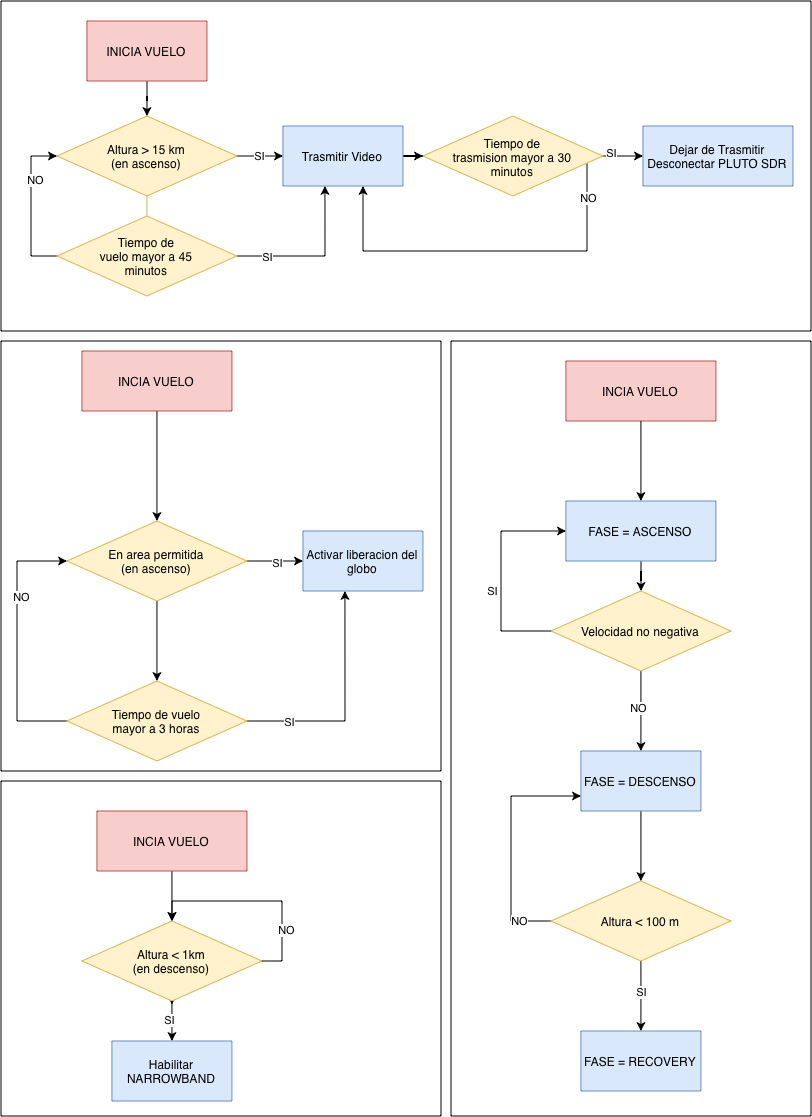
\includegraphics[width=4.9493in,keepaspectratio]{./imagenes/image40.png}

El control del payload se organiza mediante dos máquinas de estado que operan en paralelo:

\begin{itemize}
\item
  Fase de Vuelo: Define la etapa global en la que se encuentra la misión mediante la secuencia
\item
  Transmisión de Video: Define de manera independiente si el payload se encuentra transmitiendo video
\end{itemize}

Ambas máquinas de estado, la fase de vuelo y el estado de la transmisión de video, pueden variar de forma independiente. Por ejemplo, es posible que la transmisión de video se active cuando el globo ya haya iniciado su descenso tras la explosión, o que continúe operando durante dicha etapa.

\textbf{Fase de vuelo}

En cada ciclo, el sistema toma la altitud (GPS) y el timestamp de la última lectura, y evalúa la transición correspondiente según el estado actual. Los estados posibles y sus transiciones son:

\begin{itemize}
\item
  \textbf{INIT (I):} si la altitud y el timestamp recibidos son válidos, se considera que el vuelo ha comenzado. Se registra el timestamp y la altitud de lanzamiento, se transiciona a ASCENT
\item
  \textbf{ASCENT (A):} En cada ciclo de control, se calcula la altura del payload y se registra la maxima altura alcanzada. Si la altura es 1000 metros menor que la altura maxima, se asume que el payload ya comenzó su ascenso y se transiciona a DESCENT
\item
  \textbf{DESCENT (D):} se verifica si la altitud actual está por debajo 100 m. De ser así, se transiciona a \textbf{RECOVERY}
\item
  \textbf{RECOVERY (R):} Se permanece en este estado hasta encontrar el payload en el fin de la mision.
\end{itemize}

\textbf{Transmisión de video}

De forma independiente a la fase de vuelo, el sistema gestiona un ciclo propio para la transmisión de video, compuesto por tres estados: sin transmisión, pre-transmisión y transmisión activa.

Mientras no se haya completado la transmisión, el sistema evalúa dos condiciones para iniciar el proceso: que el payload se encuentre en ascenso y haya superado los 13.500 metros de altitud aproximadamente, o bien que hayan transcurrido 40 minutos desde el inicio del vuelo sin haber alcanzado dicha altura. Al cumplirse cualquiera de estas condiciones, se pasa al estado de pre-transmisión. Este estado de pre-transmisión permite avisarle a la estación terrena que se está próximo a trasmitir video.

Transcurridos 5 minutos desde ese instante, el Control Thread le indica al Video Thread que comience a transmitir.

Una vez cumplidos 30 minutos de transmisión continua, el Control Thread le indica al Video Thread que detenga la transmisión, marca la transmisión como finalizada y pasa al estado IDLE ya no se vuelve a evaluar el reinicio de la transmisión.

\textbf{Liberación del globo}

Mientras el payload se encuentre en fase de ascenso, se verifica en cada ciclo si la posición geográfica actual del payload se encuentra fuera del área de vuelo permitida, o si el tiempo total de vuelo ha superado las 3 horas. Ante cualquiera de estas dos condiciones, se acciona el mecanismo de liberación del globo y se registra el evento, para que no se siga evaluando estas condiciones.

\textbf{Activación de telemetría de respaldo}

Durante la fase de descenso, se verifica en cada ciclo si la altitud del payload se encuentra en 1000 metros o menos sobre la superficie. Al cumplirse esta condición, se activa el NarrowBand IoT con el objetivo de transmitir por la Red IoT la localización del payload tras el aterrizaje, ya que se pierde la línea de vista para la transmisión de telemetría por LoRa

\subsubsection{Almacenamiento Local}\label{almacenamiento-local}

El payload guarda en disco dos tipos de información, según si cambian o no entre reinicios: los datos de sesión (uno por arranque) y el estado de vuelo (persistente, único para todo el vuelo).

\subsubsection*{Datos de sesión}\phantomsection\label{datos-de-sesiuxf3n}

Cada arranque del sistema genera un conjunto nuevo de tres archivos, todos identificados con el mismo identificador de sesión.

\begin{itemize}
\item
  \textbf{Logs}: Guarda el registro de eventos del sistema escrito por todos los hilos del sistema a medida que ocurren sus propios eventos..
\item
  \textbf{Telemetría}: Guarda un paquete por cada ciclo de muestreo.
\item
  \textbf{Video}: Guarda el stream de video continuo de la cámara a medida que la cámara va entregando cada bloque de datos en formato TS. La grabación continúa incluso si el enlace de trasmicion está apagado.
\end{itemize}

\subsubsection*{Estado de vuelo}\phantomsection\label{estado-de-vuelo}

A diferencia de los tres anteriores, este archivo es único y persiste entre reinicios: no se crea uno nuevo por sesión, sino que se actualiza sobre el mismo archivo durante todo el vuelo. La escritura es atómica, se escribe primero una copia temporal, se fuerza su escritura física a disco, y recién entonces se reemplaza el archivo definitivo. Esto garantiza que un corte de energía a mitad de la escritura nunca deja un archivo corrupto.

\subsubsection{Gestión de Energía y Apagado de Componentes}\label{gestiuxf3n-de-energuxeda-y-apagado-de-componentes}

Gestion de Energia: Apagar SDR: Desactivar la conexion a ADALM-Pluto SDR cuando sea necesario reducir consumo (en el descenso)

\textbf{Otros Requerimientos}

\begin{itemize}
\item
  Arranque el sistema cuando se enciende la Raspi, retomando el estado en el que estaba antes de prenderse
\end{itemize}

\section{Sistema de energía}\label{sistema-de-energuxeda}

\subsection{Energy Budget}\label{energy-budget}

PONER TABLA

\subsection{Baterias}\label{baterias-1}

Los equipos de los proyectos Horus y SF-HAB utilizaron pilas primarias Energizer Lithium AA debido a su buen desempeño a bajas temperaturas \cite{ref19,ref20,ref44}. Estas baterías son de tipo primario y utilizan un sistema químico basado en litio y disulfuro de hierro (Li-FeS₂). Presentan un rango de temperatura de operación de -40 °C a 60 °C \cite{ref100} comparable al de las baterías presentadas en \cite{ref39}. Entre sus principales ventajas se encuentran \cite{ref100}:

\begin{itemize}
\item
  \textbf{Voltaje consistente:} presentan una curva de voltaje relativamente plana, típicamente entre 1,3 V y 1,5 V durante la mayor parte de su vida útil. Cuando le queda muy poca energía (después de entregar aproximadamente 3000 - 3500 mAh), el voltaje experimenta una caída muy rápida y pronunciada. Las pruebas de rendimiento de la industria consideran que la batería está "agotada" o con poca carga funcional cuando alcanza los 0.8 voltios.
\item
  \textbf{Alto desempeño de potencia:} está diseñada para soportar una demanda de corriente continua de hasta 2.5 amperios y pulsos de hasta 4.0 amperios (en ciclos de 2 segundos encendida y 8 segundos apagada).
\item
  \textbf{Alta capacidad bajo carga alta:} mantiene la capacidad aunque aumente la descarga.
\end{itemize}

Además, ofrecen una mayor capacidad energética por kilogramo que las baterías de ion-litio 18650 utilizadas por \cite{ref2} con valores de aproximadamente 300 Wh/kg y 180 Wh/kg, respectivamente \cite{ref101}.

Por otro lado, si bien las baterías de cloruro de tionilo-litio (LiSOCl₂) ofrecen la mayor energía utilizable por kilogramo \cite{ref102} y permiten operar a temperaturas más bajas \cite{ref39} presentan el problema de la pasivación. Este fenómeno consiste en la formación de una película aislante sobre la superficie del ánodo de litio, producto de la reacción entre el cloruro de tionilo y el litio. En aplicaciones que requieren pulsos de corriente elevados, esta capa de pasivación puede limitar el desempeño de la batería \cite{ref103}.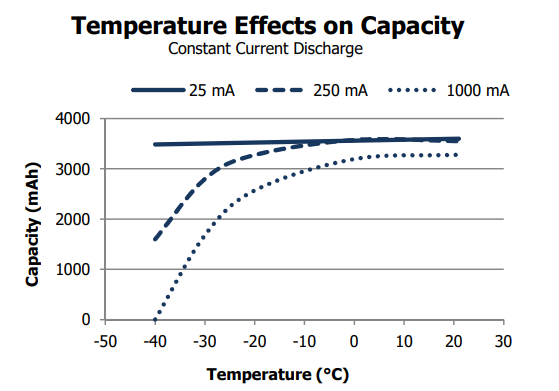
\includegraphics[width=3.3281in,keepaspectratio]{./imagenes/image34.png}

Hablando con Richard Corbo, quien tuvo varias expediciones a Antártida, nos comentó que la capacidad de la batería se reduce drásticamente a temperaturas muy bajas. Contó que su celular se quedaba sin batería mucho antes de lo normal, principalmente porque las temperaturas eran muy bajas. Viendo el datasheet de las baterías L91, se puede observar este comportamiento, a medida que baja la temperatura, baja la capacidad. Este fenómeno ocurre en las baterías en general porque, a temperaturas bajas, la actividad química disminuye \cite{ref104}.

Se seleccionaron las baterías Energizer Lithium AA porque presentan un desempeño adecuado y cuentan con antecedentes de uso exitoso en proyectos amateur de globos estratosféricos. Además, se va a emplear un mecanismo para que la temperatura de las baterías no baje significativamente con respecto a la temperatura ambiente en la superficie.

\subsection{Banco de baterias}\label{banco-de-baterias}

Para el sistema de componentes se debe generar un suministro de 5V con una capacidad de aproximadamente 9000 mAh, utilizando las baterías de 1.5V con una capacidad de 3000mAh. Para aumentar el voltaje del banco de baterías se van a juntar baterías en serie. Como no es posible hacer un banco de 5V utilizando baterías de 1.5V se va a utilizar un conversor reductor o elevador para ajustar el voltaje. Para maximizar la eficiencia en la conversión y minimizar la acumulación de calor, la mejor opción es el conversor reductor.

Se debe tomar en cuenta que a mayor demanda de corriente, el voltaje disminuye debido al aumento de la resistencia interna de la celda \cite{ref105}. Además, antes de haber entregado 3000 - 3500 mAh, presenta una caída en voltaje de aproximadamente 10 - 15\% (teniendo una descarga de entre 600 - 1000 mA). Para tomar en cuenta la disminución de voltaje debido a la elevada carga y la disminución de la capacidad, se va a prever un margen de voltaje mayor.

Con un banco de 6V, se prevé una caída de hasta 5.1 - 5.4V. Estos voltajes no dejan un margen suficientemente alto para mitigar otras posibles causas de caída en voltaje (temperatura, picos de consumo inesperados, etc). Además, debe quedar suficiente energía para que el sistema de encontrado del dispositivo quede activo durante X horas posteriores a aterrizar. Para un banco de 7.5V se puede prever una caída de hasta 6.375 - 6.75V, dejando un buen margen en caso de imprevistos. Se determina que se va a construir un banco con 5 baterías en serie.

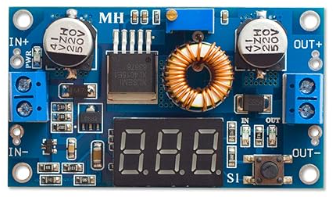
\includegraphics[width=2.8698in,keepaspectratio]{./imagenes/image21.png}

El conversor HiLetgo XL4015 (5A) tiene una eficiencia de hasta 96\% (Dependiendo del voltaje de entrada/salida, corriente y presión atmosférica) \cite{ref106}. Suponiendo una eficiencia de aproximadamente 93\%, la potencia que entrega el banco de baterías se calcula haciendo \(P_{Salida} = \ P_{entrada}\ .\ 0.93\). Para la salida se requieren 15W (5V, 3000mA como máximo). Entonces, la potencia de entrada son aproximadamente \(16.1W\). Con un banco de 7.5V, las baterías van a descargar aproximadamente 2.15A.

Para aumentar la capacidad, se conectan sub bancos (conjunto de baterías en serie) de baterías en paralelo. Además, ayuda a repartir la carga entre todos los sub bancos. Para complir con los requerimientos, se utilizara un banco de 5S3P. Esta configuración permite distribuir la carga y tener margen por caídas de voltaje.

En el laboratorio se verificó el correcto funcionamiento del reductor utilizando una fuente y un medidor. Se calibró girando el tornillo del trimpot.

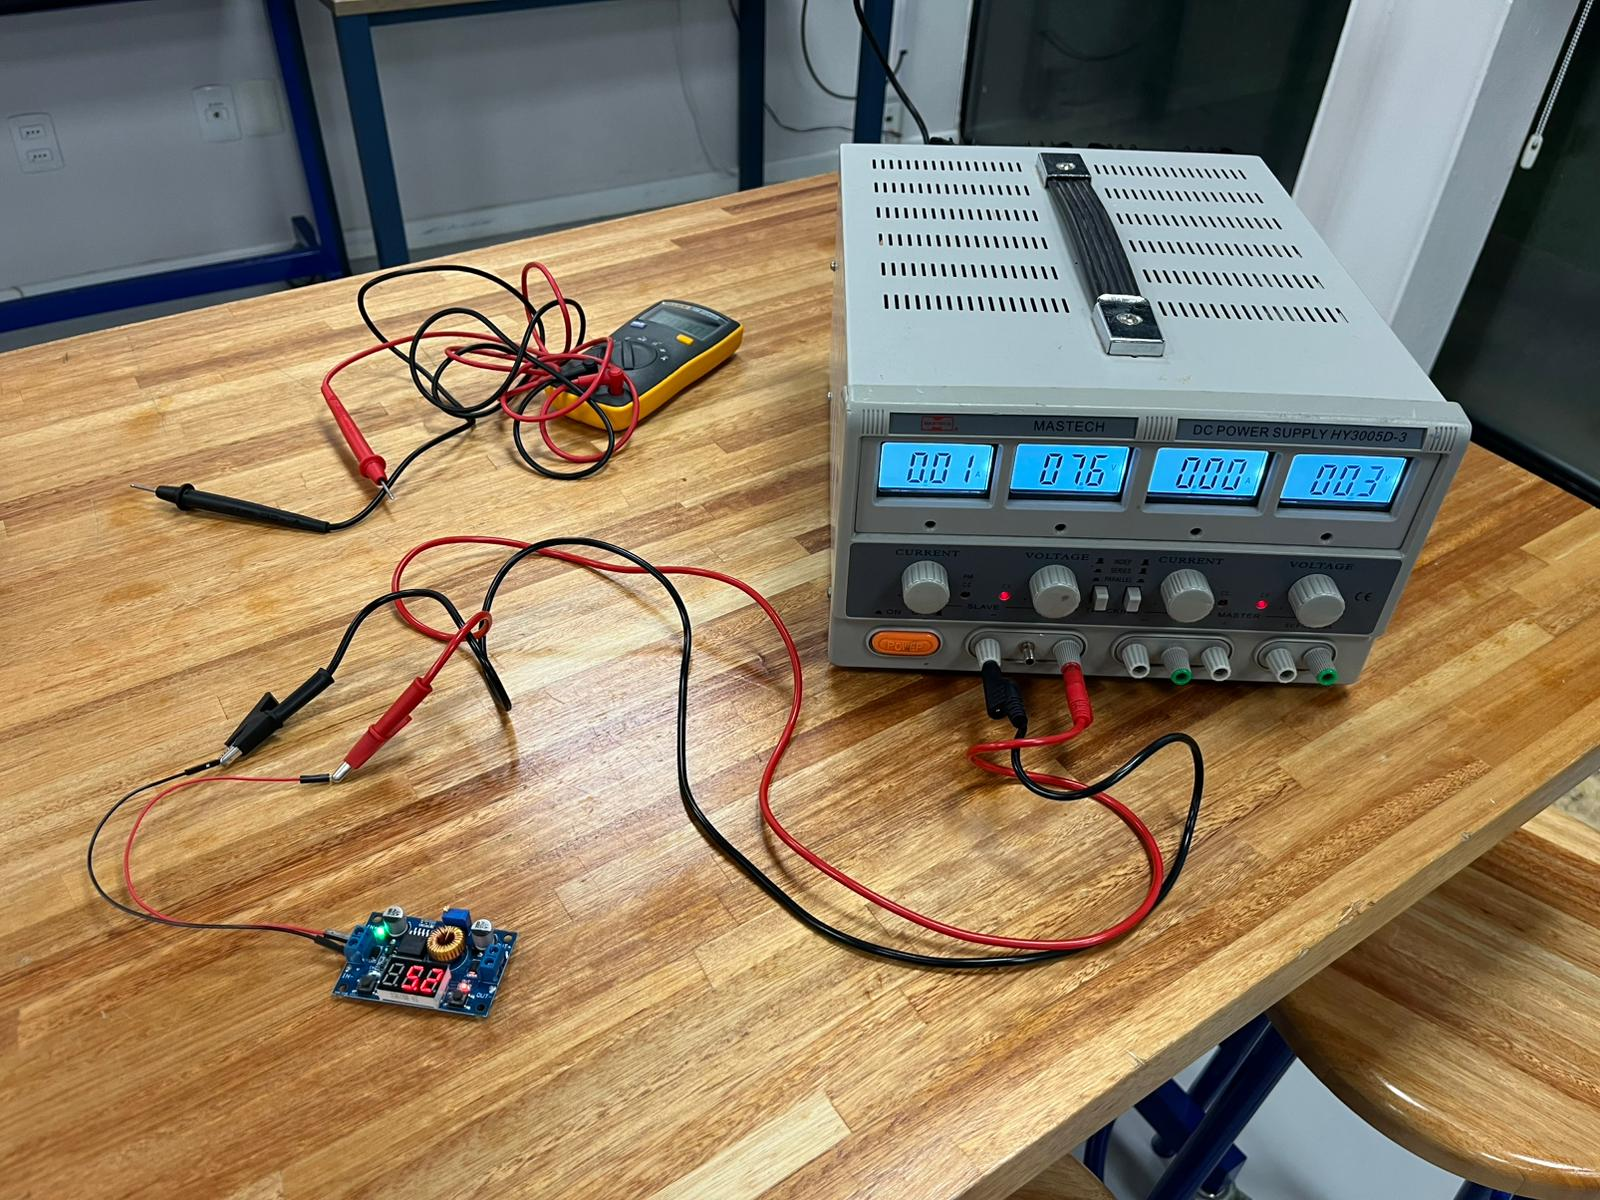
\includegraphics[width=2.8899in,keepaspectratio]{./imagenes/image72.png}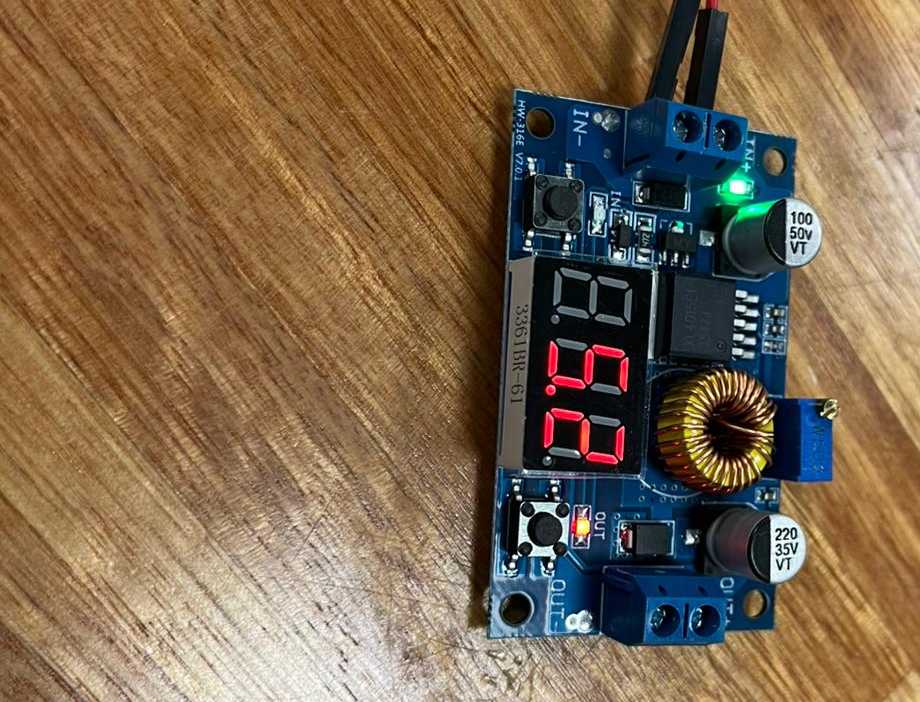
\includegraphics[width=2.8975in,keepaspectratio]{./imagenes/image8.png}

\subsection{Arquitectura}\label{arquitectura}

\section{Estructura e integración}\label{estructura-integracion}

\subsection{Materiales y estructura}\label{materiales-estructura}

En \cite{ref2} utilizaron una carcasa de aluminio 6061 para la disipación de calor que genera un transmisor de 5Ghz. Utilizaron el aluminio porque es ligero. Además, esqueletizaron algunas caras para disminuir aún más el peso del sistema. En las caras restantes, se fijaron los componentes utilizando separadores de aluminio. Proporcionando un camino directo de conducción para transferir el calor generado por los componentes hacia el aluminio.

Adicionalmente, las caras de mayor superficie que no fueron esqueletizadas presentaban una superficie altamente reflectiva. De este modo, la carcasa no sólo disipa el calor generado internamente, sino que también reduce la absorción del calor incidente en forma de luz.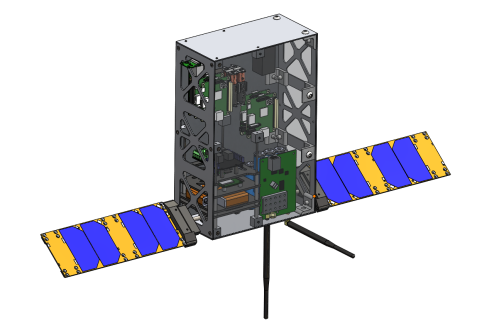
\includegraphics[width=2.7267in,keepaspectratio]{./imagenes/image35.png}

En \cite{ref32} utilizaron aluminio para el exterior y poliestireno expandido para el interior de la estructura. El aluminio les permitió tener un diseño fuerte y robusto, pero a costo sobre el presupuesto de peso. Por otro lado, les fue conveniente por lo liviano que es. Además, porque es barato y proporciona cierto aislamiento térmico que el aluminio no ofrece. \cite{ref2} no explica específicamente porque combina las dos, pero se supone que redujeron la cantidad de aluminio y adicionaron poliestireno para mantener la durabilidad y mejorar el aislamiento térmico que es importante para componentes como las baterías.

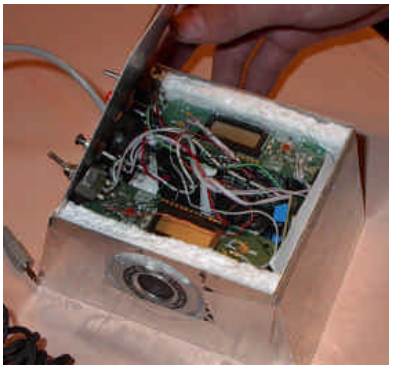
\includegraphics[width=2.7284in,keepaspectratio]{./imagenes/image63.png}

En \cite{ref3} utilizaron poliestireno expandido para la capa interna de la estructura para proporcionar aislación térmica. Para el prototipo no utilizaron aluminio, pero igualmente construyeron una estructura de aluminio como los establece el estándar del CubeSat para hacer pruebas en el laboratorio. Aclararon que las opciones más comunes para CubeSats son los tipos 5005, 5052, 6061, 7075 de aluminio. Terminaron usando PLA para la capa externa.

Para la estructura se implementará un sistema de gestión térmica pasivo y activo. El pasivo no implica el uso de energía, es de bajo costo, volumen y riesgo. En Uruguay no es posible conseguir aluminios de los tipos que establece el estándar CubeSat sin invertir más de lo que se está dispuesto, por lo que se va a resolver con aluminio que se venden en joyerías. Se utilizará aluminio para la capa externa con el objetivo de darle rigidez, absorber y retener el calor generado por componentes, y reducir el calor incidente. Para mantener la temperatura interior dentro de los valores operativos de los componentes, se utilizará una capa de Poliestireno Expandido. Los componentes que más generan calor (amplificadores, transmisores, etc) y que sobrevivan temperaturas bajas, se colocarán contra el aluminio para disipar el calor por conducción. Para el sistema activo, se utilizará el calor que genera el transmisor LoRa E22-400T22S. Se implementará un disipador para aumentar/mantener la temperatura de las baterías. Además, se rodearán con una capa de Poliestireno adicional para asegurar que se contenga la temperatura.

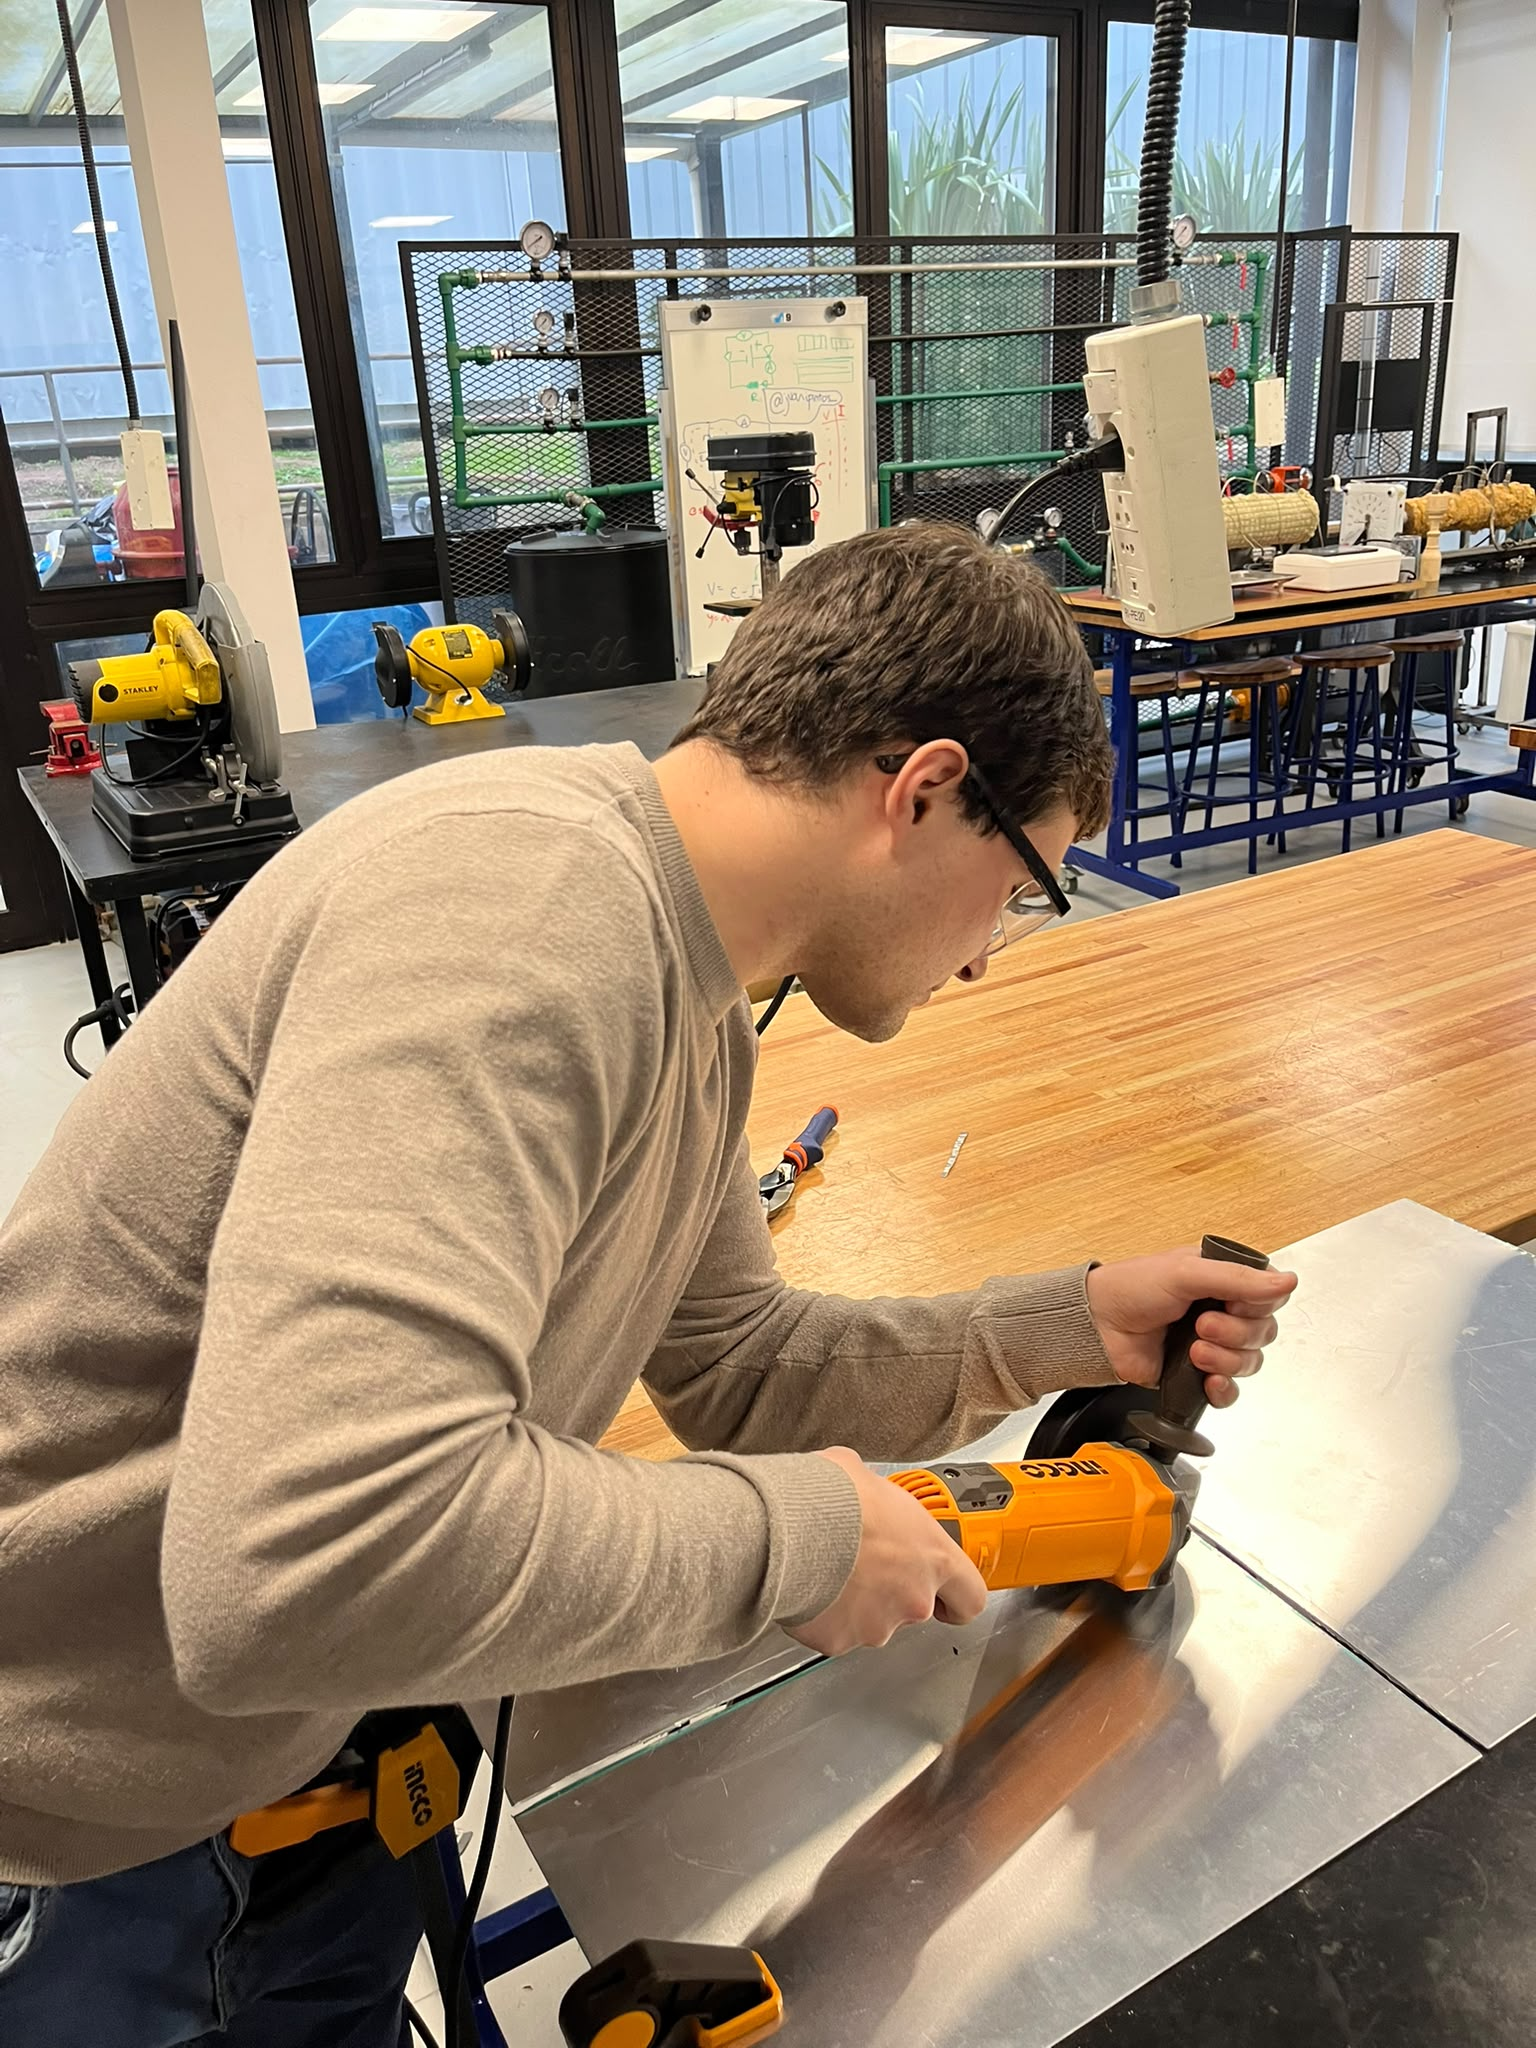
\includegraphics[width=2.8482in,keepaspectratio]{./imagenes/image56.png}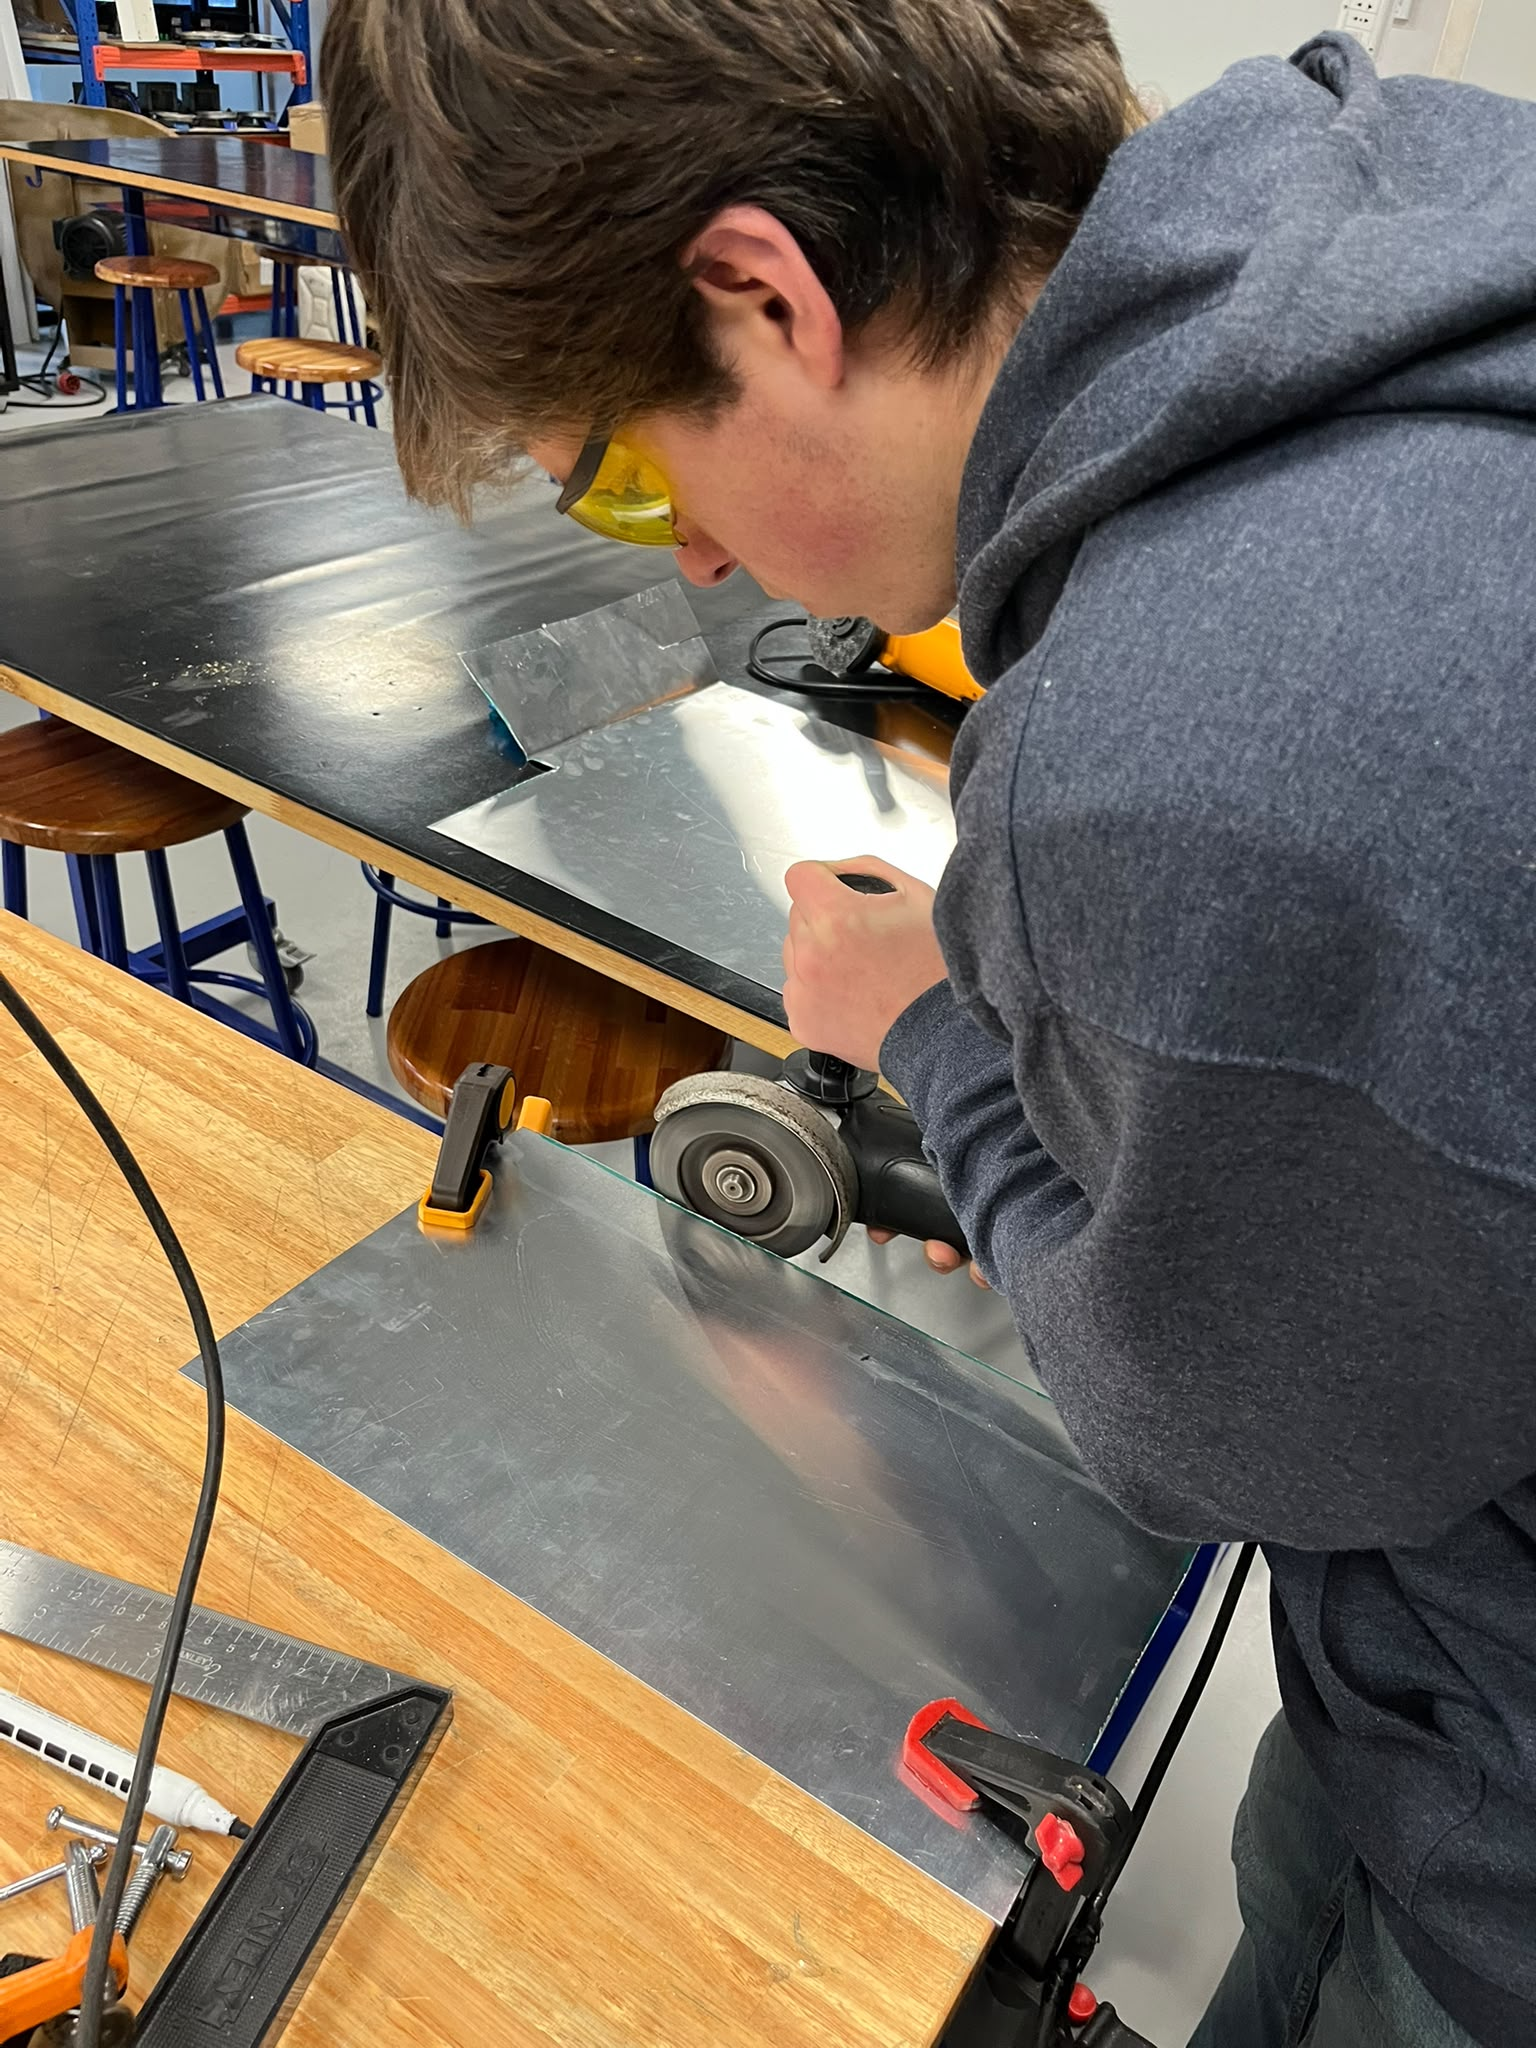
\includegraphics[width=2.8329in,keepaspectratio]{./imagenes/image75.png}

\subsection{Diseño térmico}\label{diseno-termico}

\pendiente{Diseño térmico.}

\subsection{Transición de protoboard a placa soldada}\label{transiciuxf3n-de-protoboard-a-placa-para-soldar}

Una vez teniendo el sistema de telemetría funcionando en una protoboard, se adquirieron placas para soldar y cables con núcleo sólido para tener el sistema con conexiones permanentes y rígidas. Además, se adquirió un adaptador de pines para la RasPi, para así no tener que soldar sobre la misma y mejorar la prolijidad. Una vez finalizadas las soldaduras iniciales, se verificó el funcionamiento de la transmisión de telemetría.

Placa Payload V1:

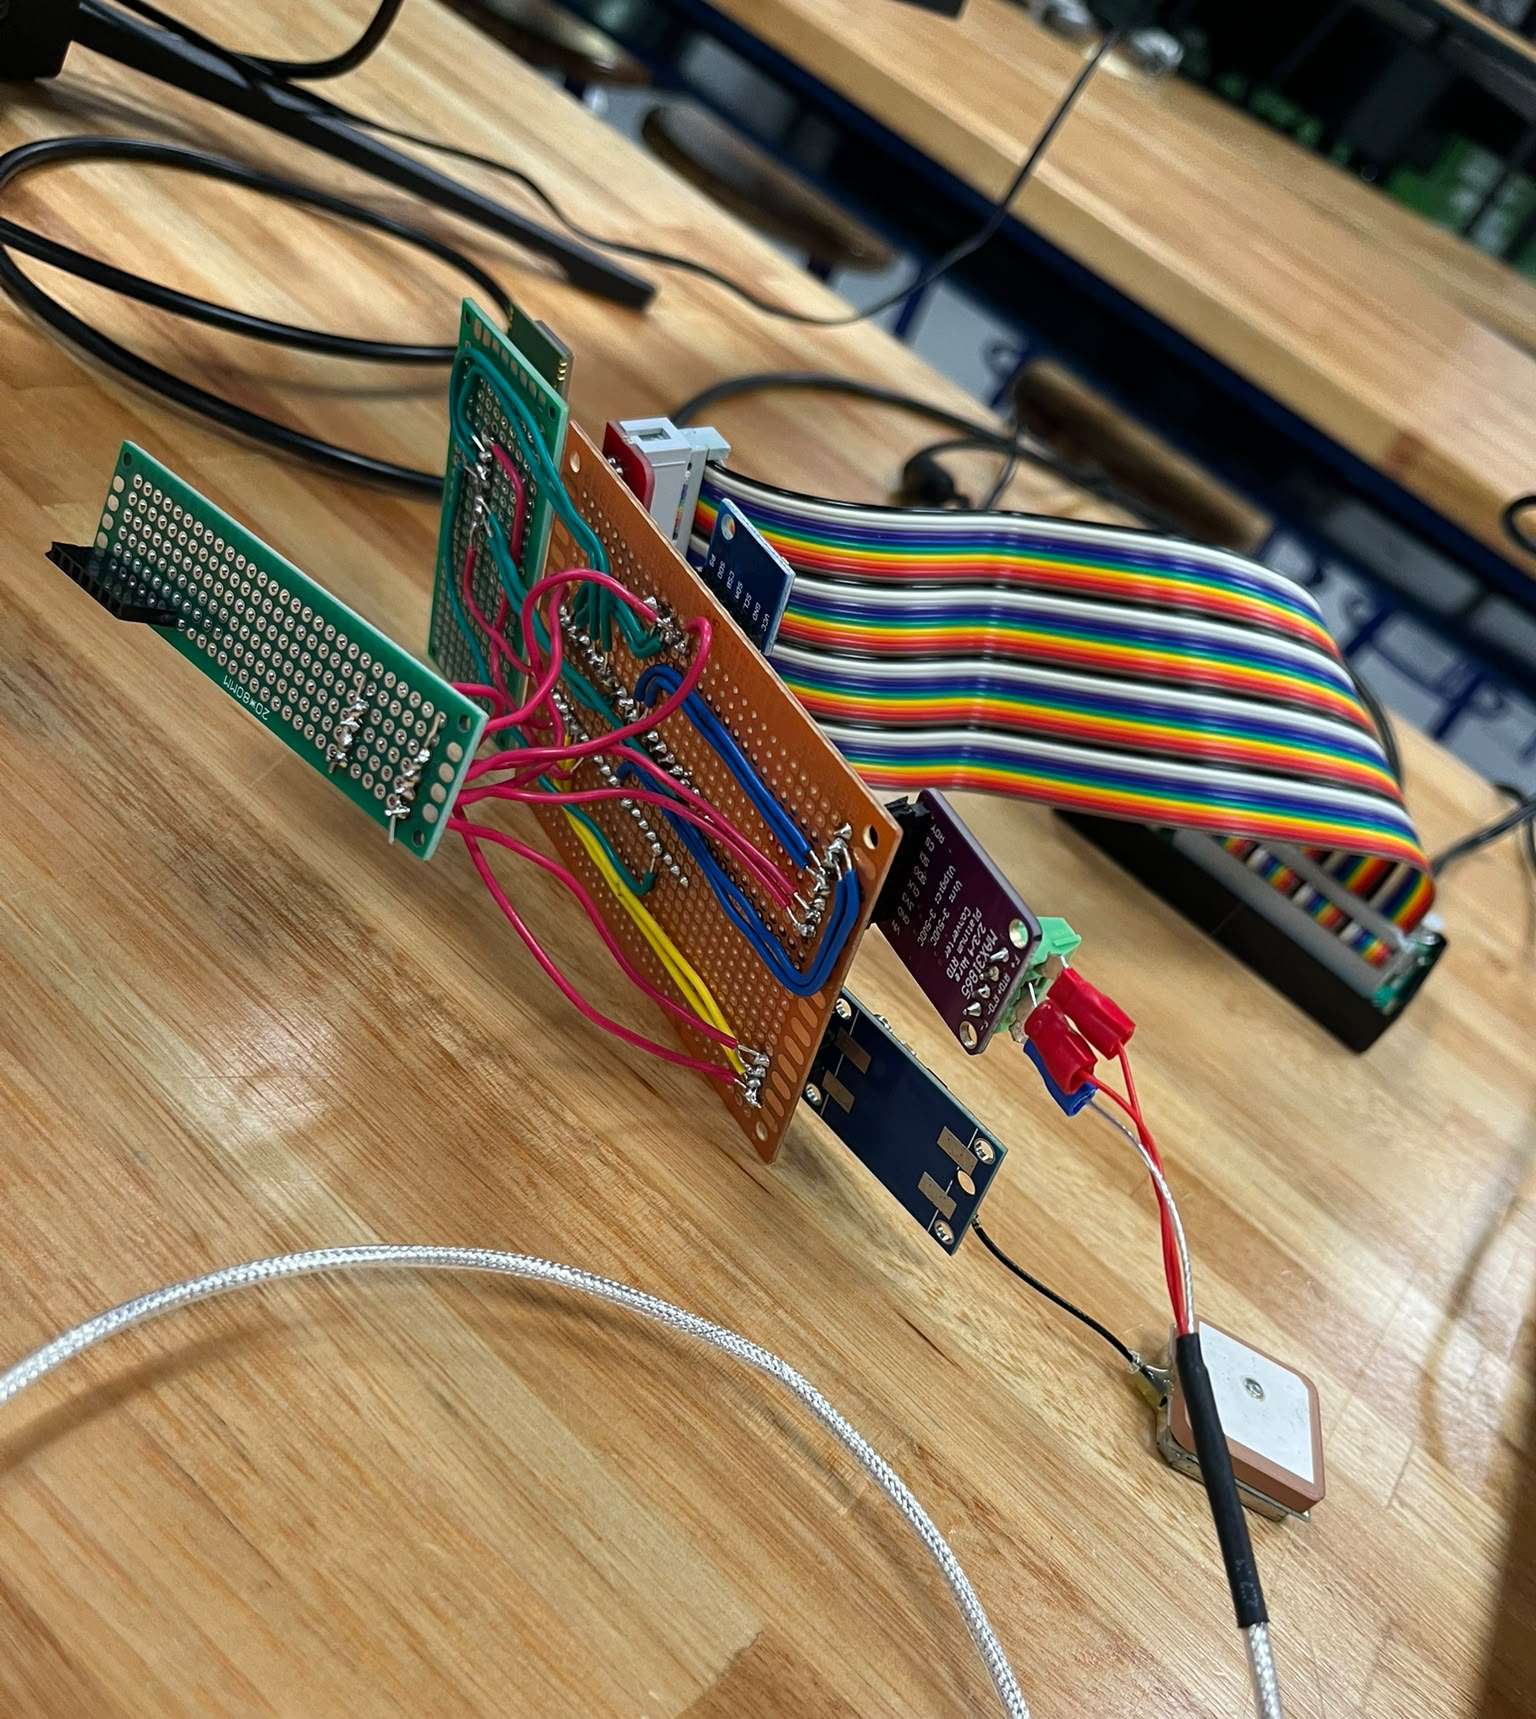
\includegraphics[width=1.5413in,keepaspectratio]{./imagenes/image24.png}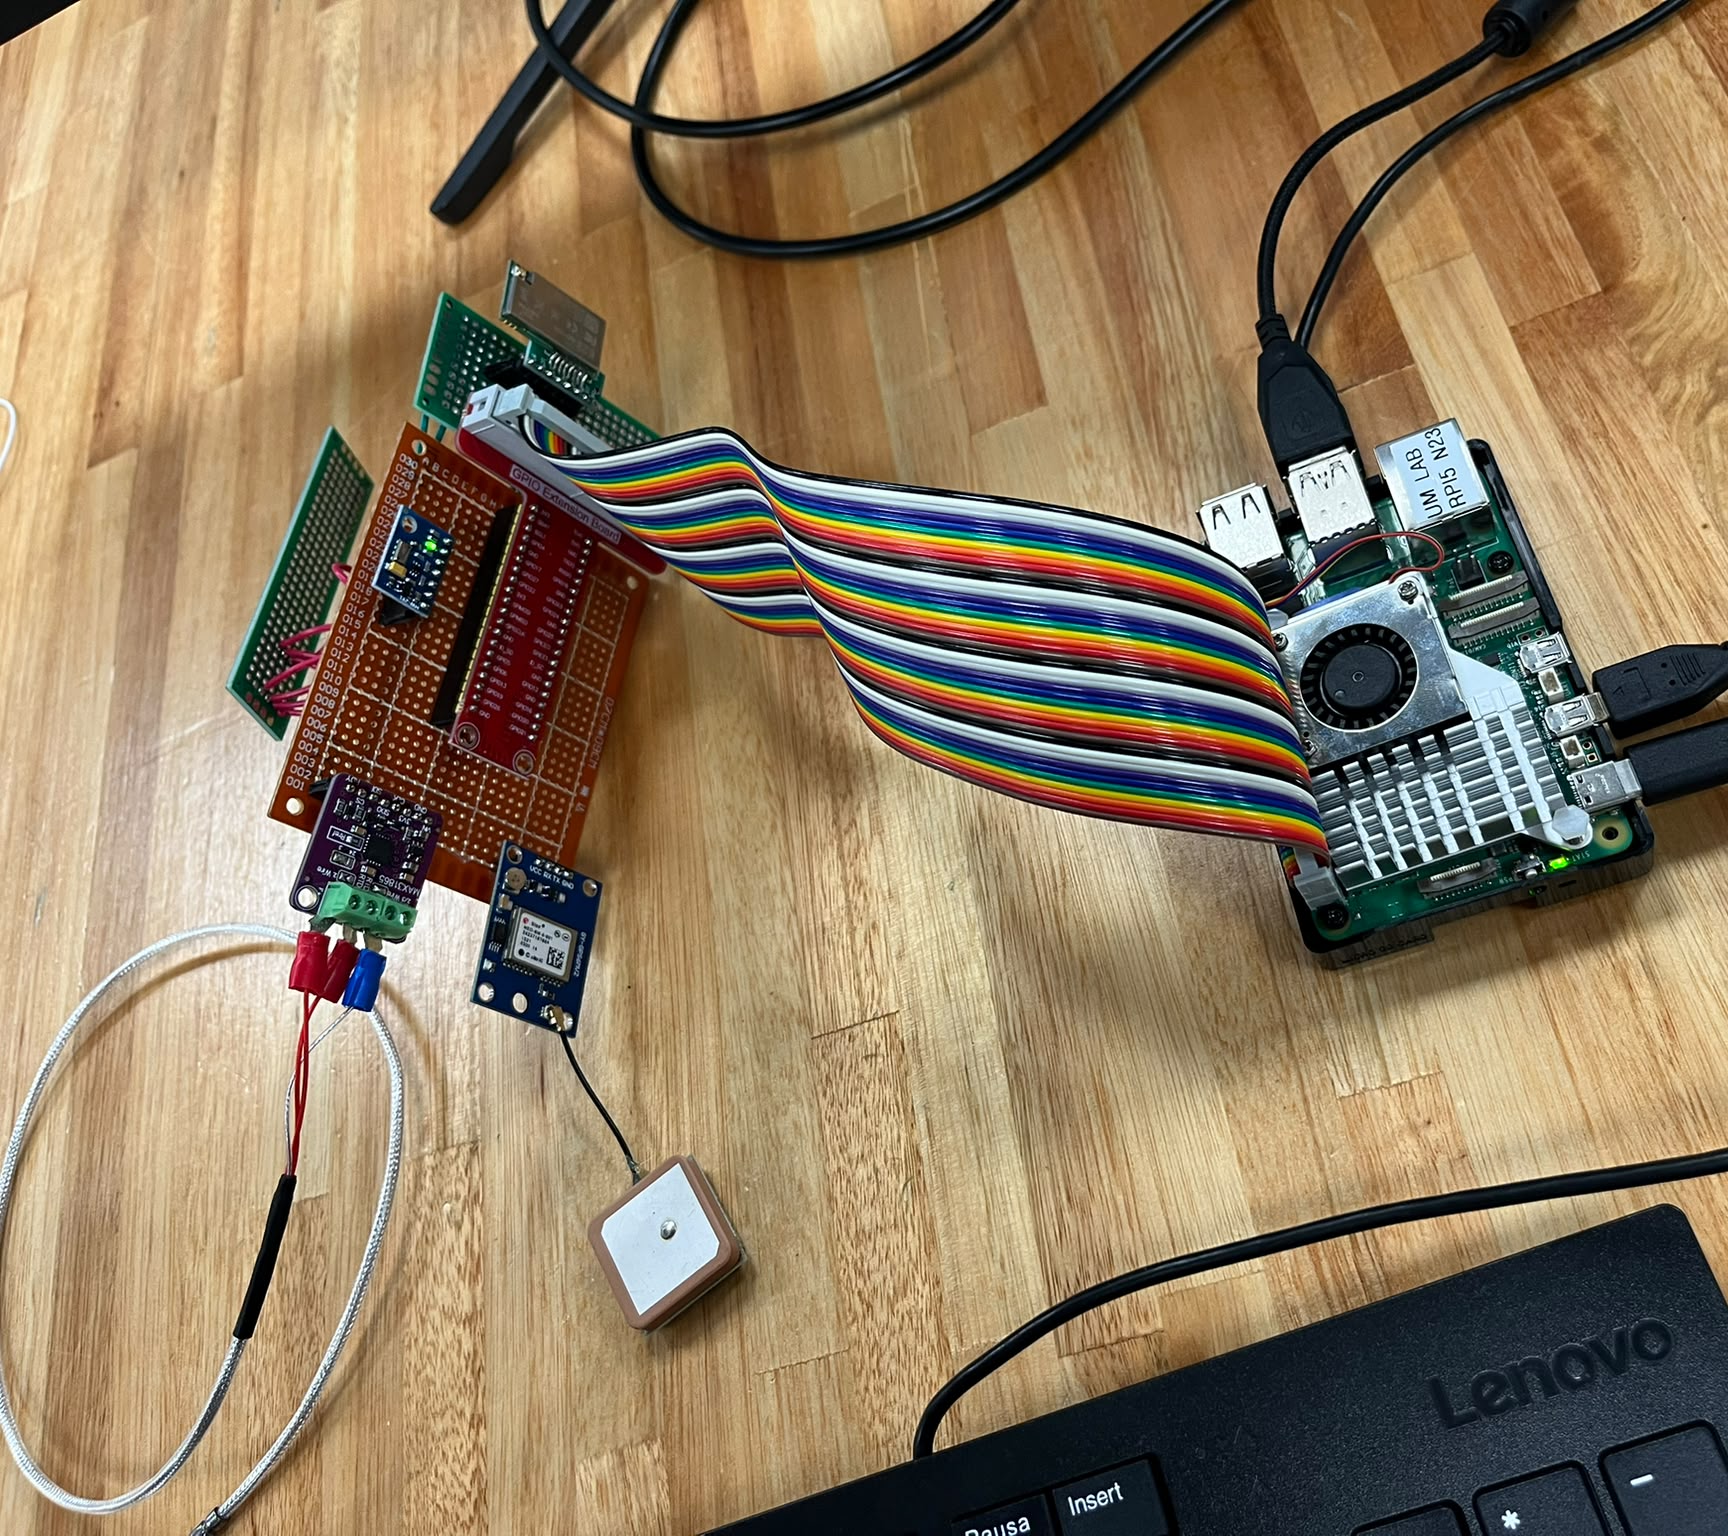
\includegraphics[width=1.9839in,keepaspectratio]{./imagenes/image23.png}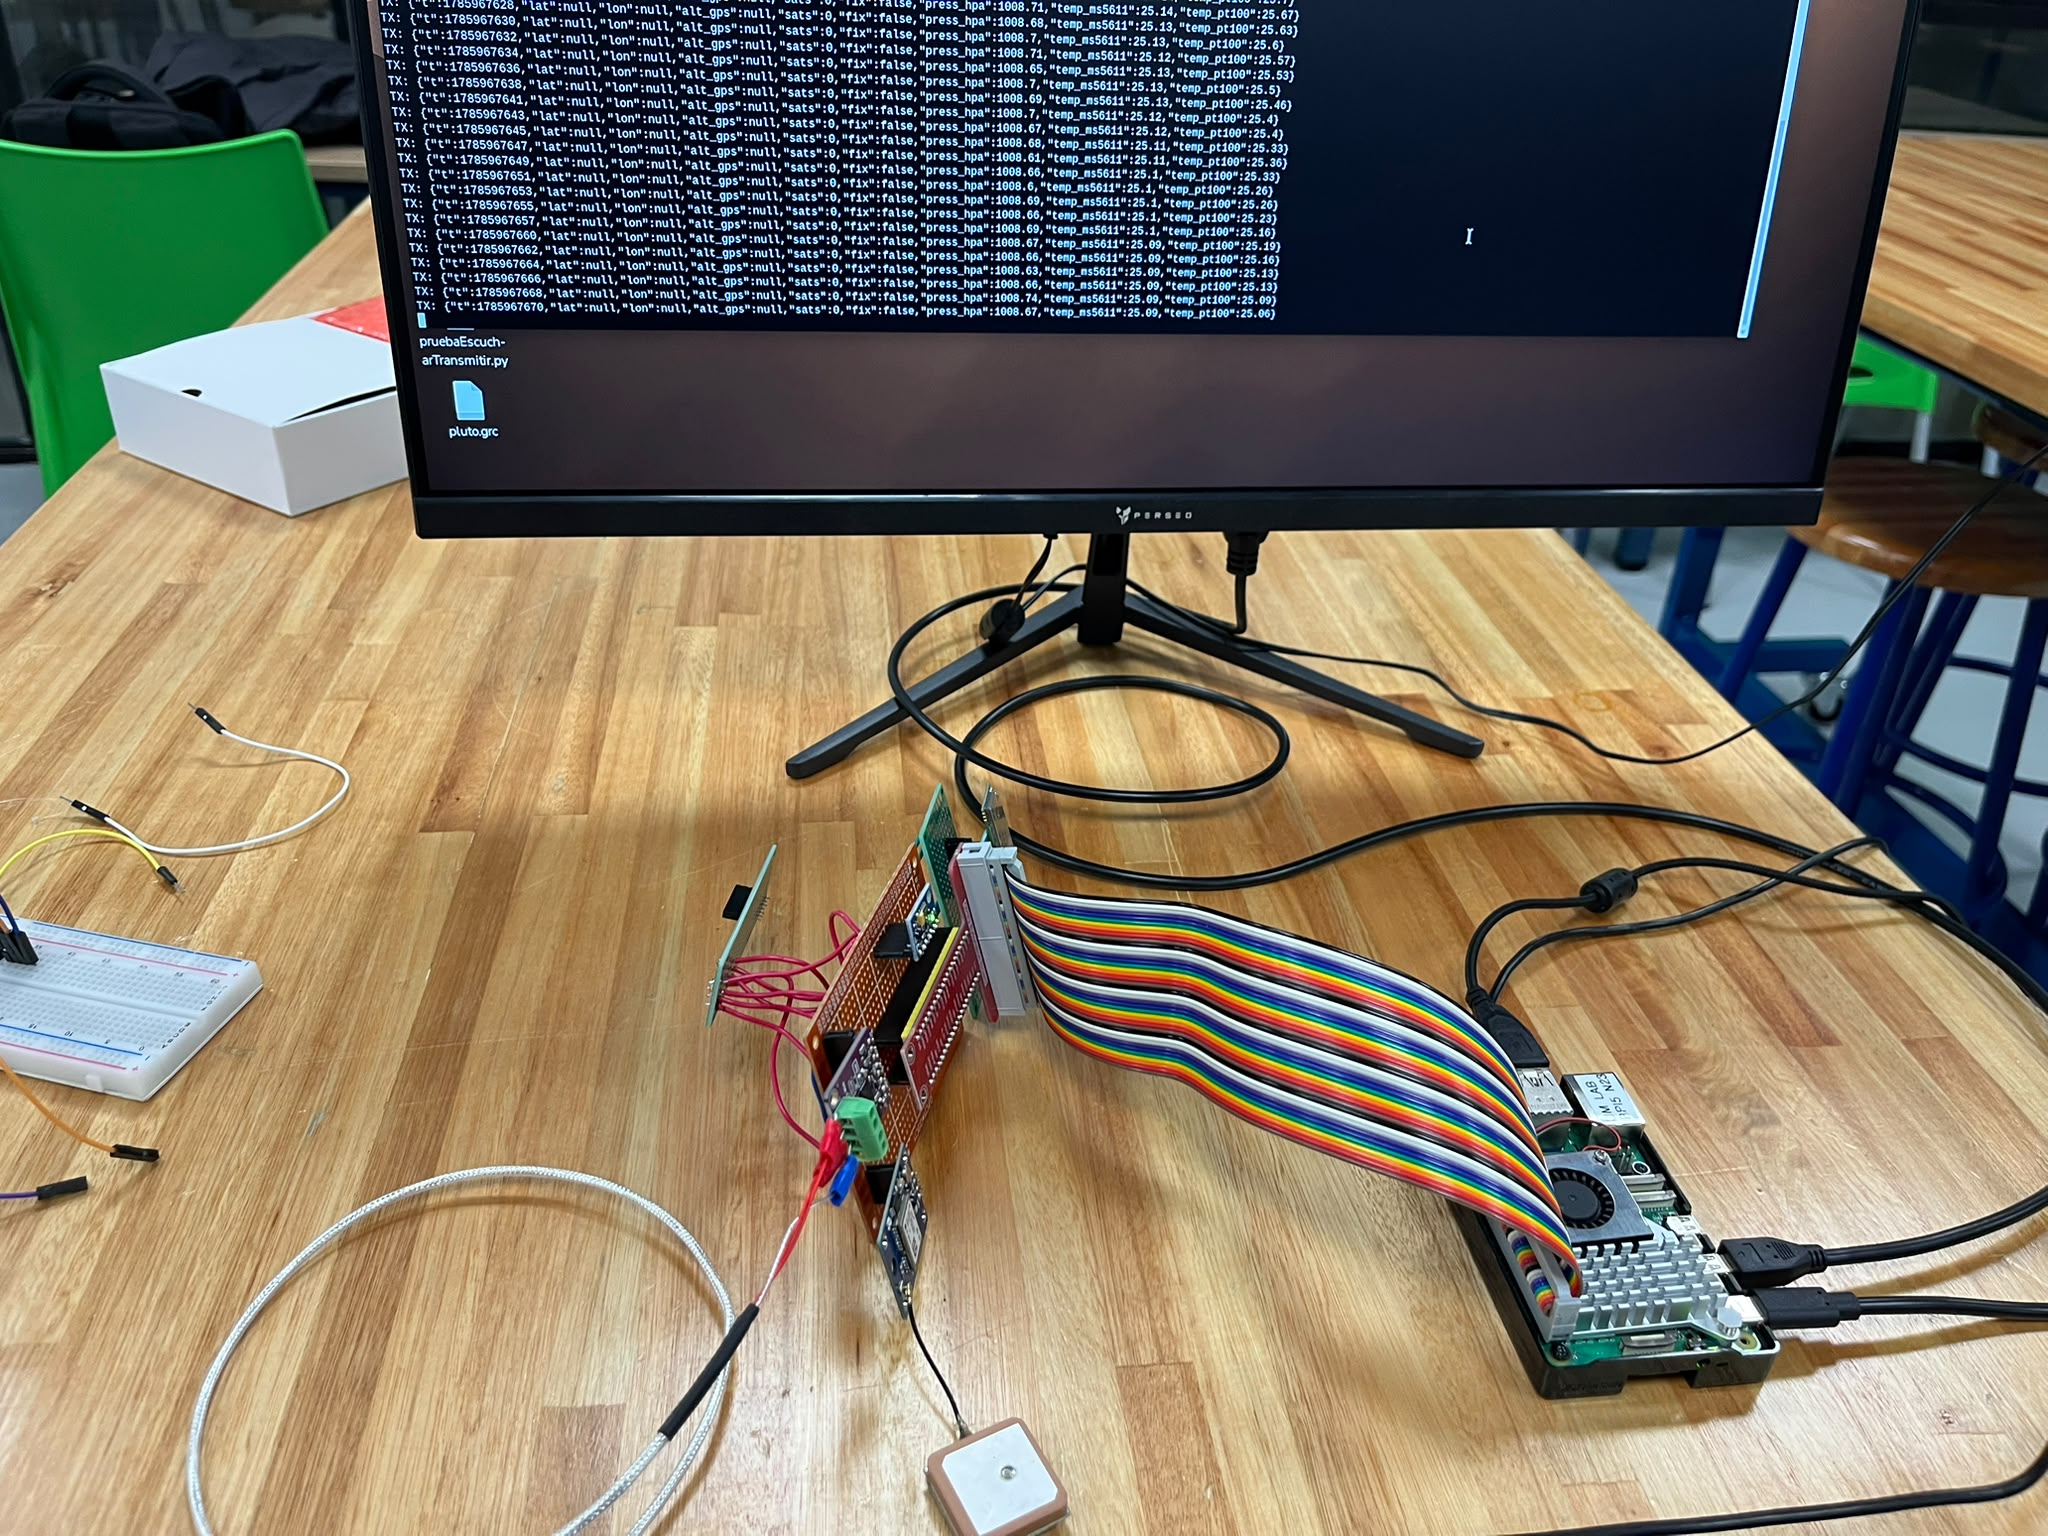
\includegraphics[width=2.2622in,keepaspectratio]{./imagenes/image87.png}

Placa Payload V2:

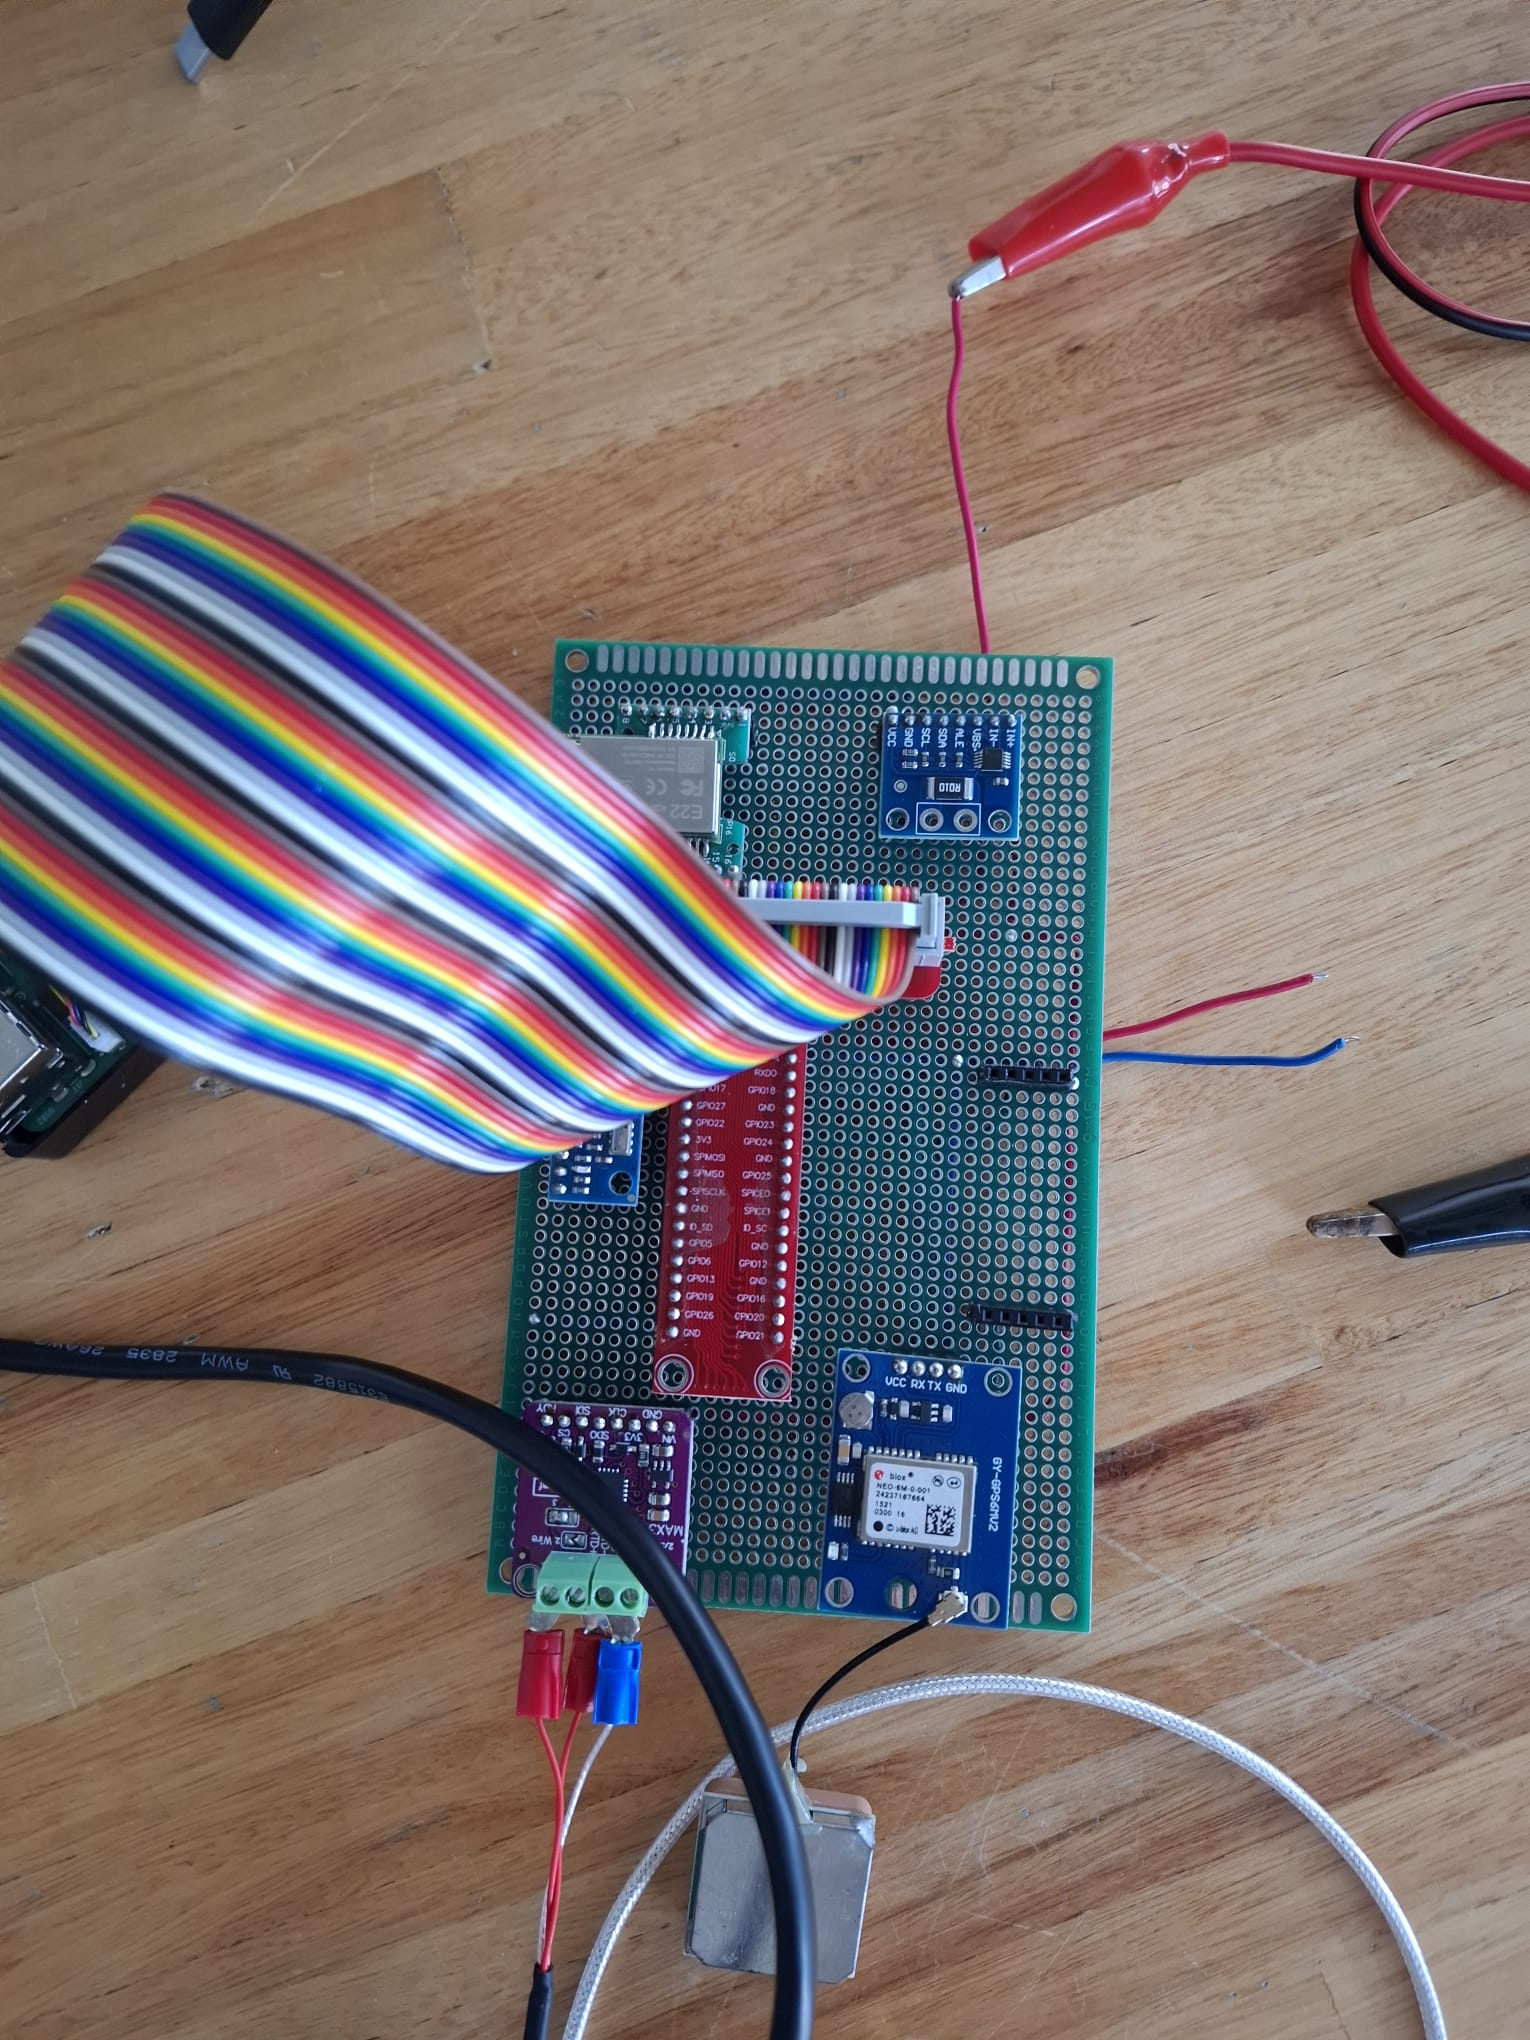
\includegraphics[width=2.0807in,keepaspectratio]{./imagenes/image95.jpg}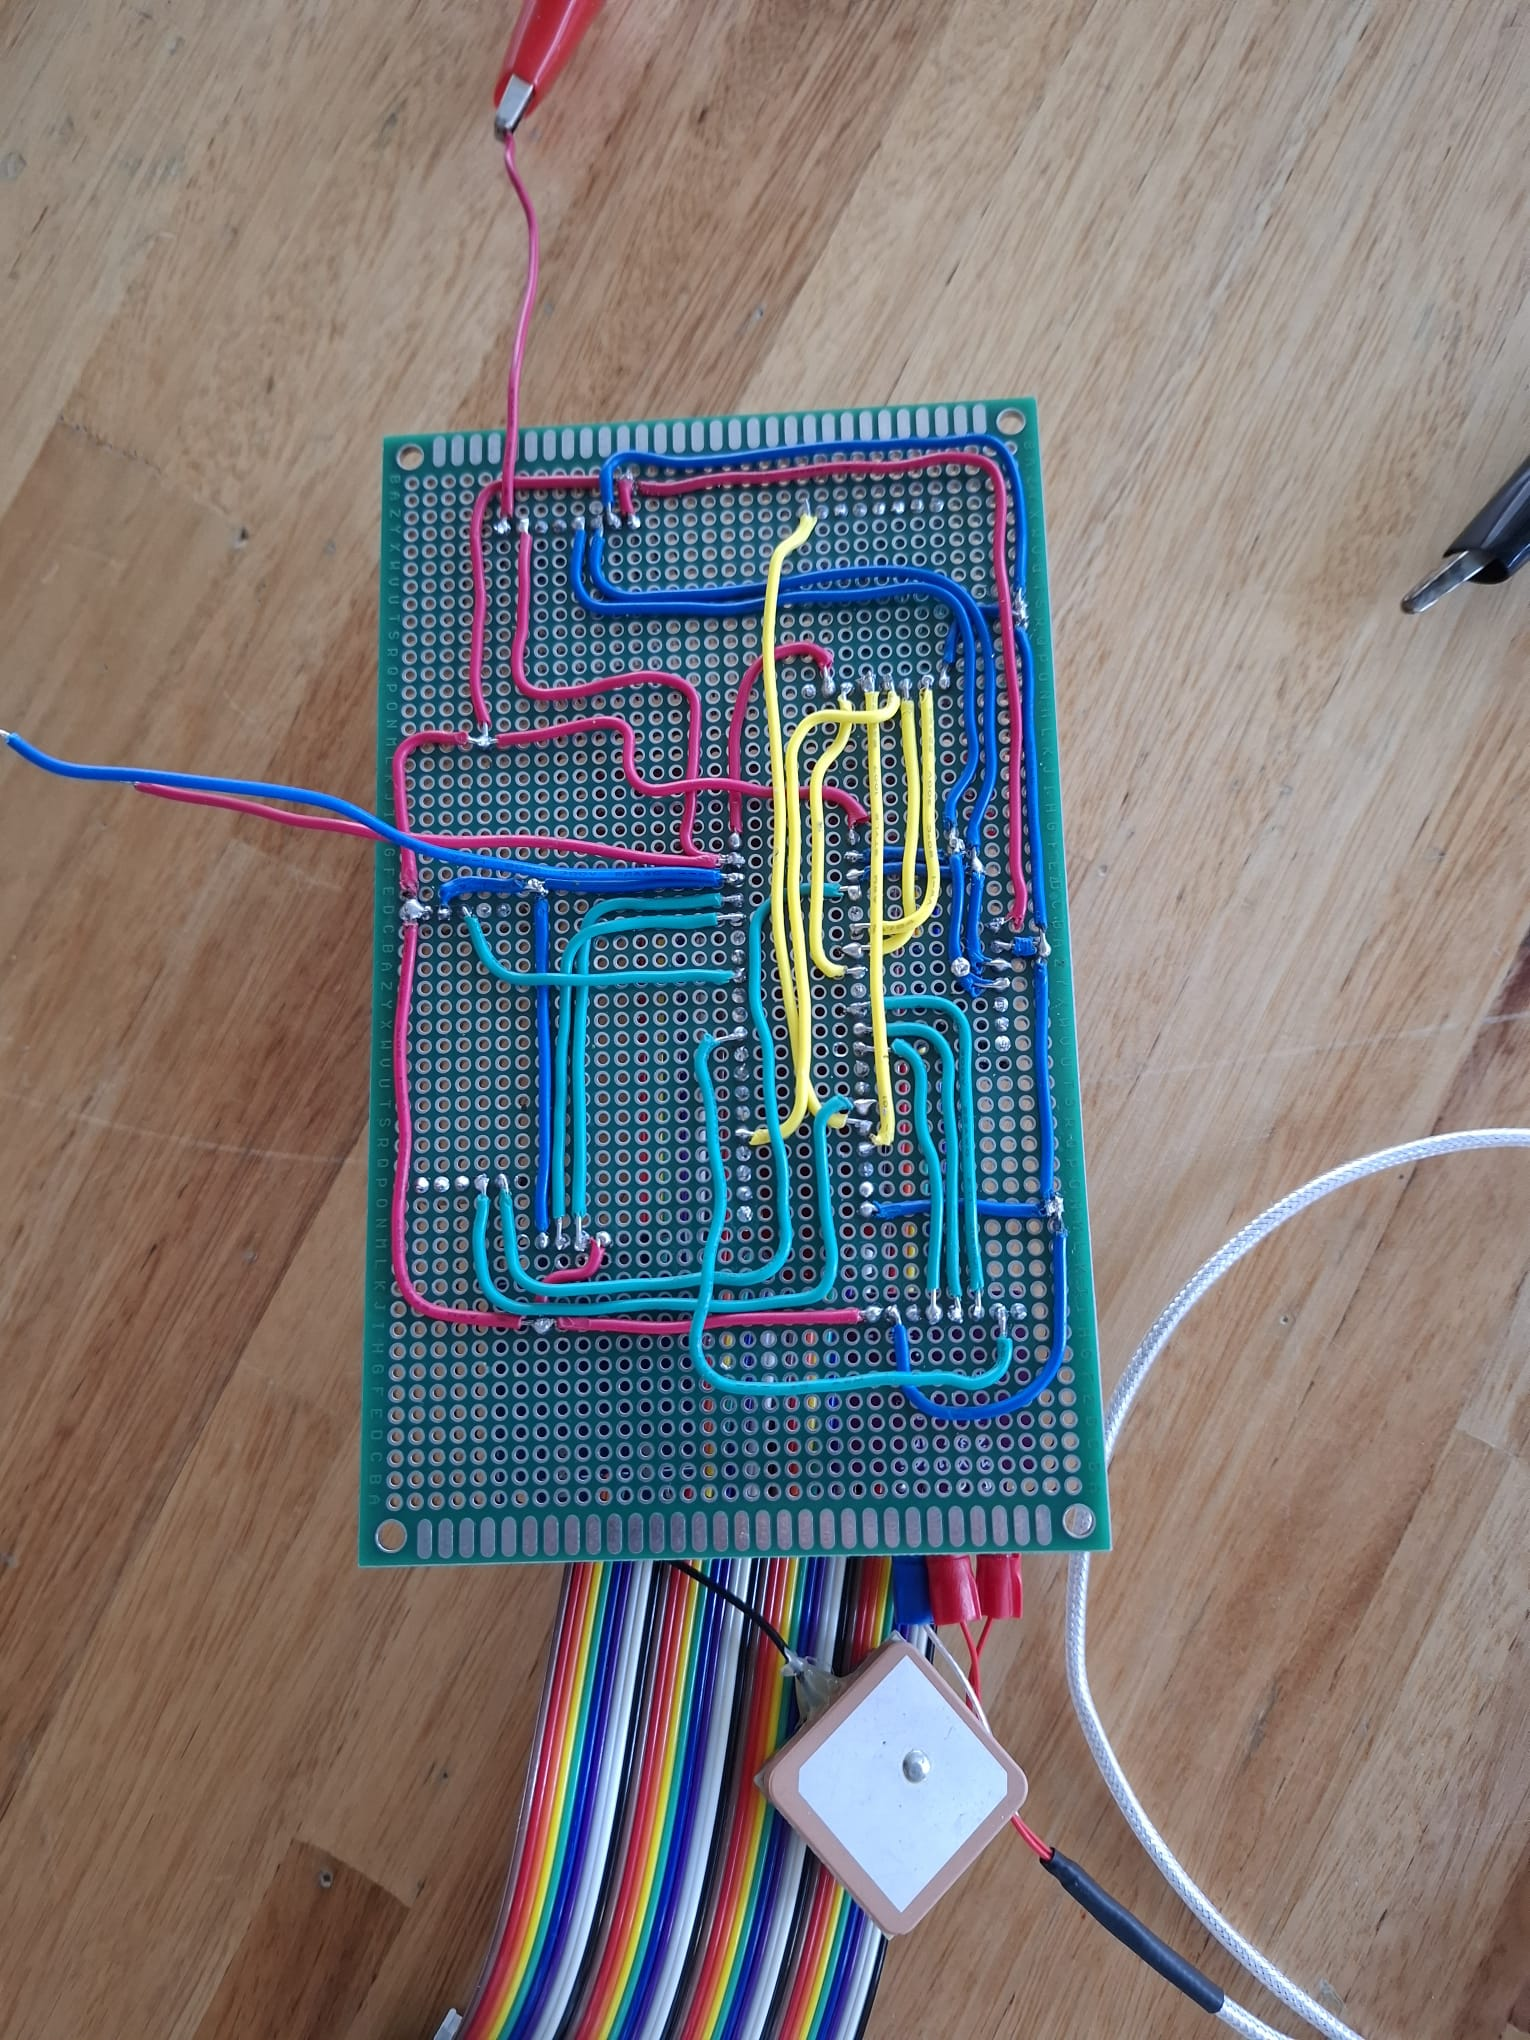
\includegraphics[width=2.0677in,keepaspectratio]{./imagenes/image74.jpg}

\section{Globo, descenso y recuperación}\label{lanzamiento}

\subsection{Weight budget}\label{weight-budget}

\subsection{Selección del globo}\label{seleccion-globo-cap}

\subsubsection{Opciones de globos}\label{opciones-de-globos}

Existen distintos tipos de globos según la altitud a la que se quiera llegar y el peso del payload. También hay distintos proveedores con precios y condiciones de envío muy diferentes. Como el presupuesto es una restricción del proyecto, la selección se hizo comparando todas estas variables.

Se compararon tres tipos de proveedores: Strato Flights, High Altitude Science y Kaymont. Son referentes mundiales en el mundo de los globos estratosféricos.

Strato Flights ofrece seis modelos de globo, desde el Pilot Balloon (payload de 30 g y altitud promedio 11,5 km) hasta el Weather Balloon 3000 (payload máximo de 3000 g y altitud 40 km). Los precios van de 15 € a 800 € según el modelo. A esto hay que sumarle el costo del envío que puede ser de hasta 60 € dependiendo el destino. El tiempo de entrega es en todos los casos entre 3 y 5 días \cite{ref76}.

Por otro lado, High Altitude Science tiene una escala de precios más baja. El globo de 350 g cuesta 40 USD. El más grande de su catálogo es el de 1500 g y cuesta 160 USD. El costo del envío depende del destino, pero solo envían a Europa y Estados Unidos. Según su información técnica el globo de 1200 g supera los 35 km de altitud \cite{ref75}.

Por último, Kaymont tiene los precios más accesibles de los tres. Un globo capaz de transportar entre 900 y 1800 g de payload cuesta 100 USD, muy por debajo de lo que cobran los otros dos proveedores. El envío a Uruguay cuesta 85 USD, mientras que a Florida, Estados Unidos, baja a 10 USD. Kaymont también ofrece una gama más amplia de tamaños de globo. Esto da flexibilidad si el peso del payload cambiará durante el desarrollo del proyecto \cite{ref76}.

\subsubsection{Selección del globo}\label{selecciuxf3n-del-globo}
El globo elegido para este proyecto es el Kaymont de 1000 gramos, fabricado por Totex (Japon) en látex natural biodegradable. Sus especificacion principales son \cite{ref77}:

\begin{itemize}
\item
  Peso del globo: 1000 g
\item
  Material: látex natural, sin conservantes. 100 \% biodegradable en 24 a 36 meses.
\item
  Gas de inflado: helio o hidrogeno grado UHP 5
\item
  Payload recomendado: 2-4 lb (907 - 1814 g), con un máximo estructural de 40 lb
\item
  Velocidad de ascenso recomendada por el fabricante: \textasciitilde5m/s
\item
  Diámetro de reventón: 25,8 ft (\textasciitilde7,9 m)
\item
  Altura de reventón estimada con el payload recomendado: 28.956-32.200 m
\end{itemize}

La decisión se tomó principalmente por la restricción del presupuesto. Comparando los tres proveedores para un payload como el que requiere este proyecto, los 100 USD de Kaymont era bastante más barato que los otros proveedores. Incluso, por temas de envío a Uruguay, éste era el que mayor facilitaba su llegada.

Además, el globo de 1000 g de Kaymont es una opción validada en la práctica. Es utilizado para el relevamiento de datos en altura por las bases del Space Force de Estados Unidos. Su velocidad de ascenso recomendada por el fabricante (\textasciitilde5 m/s) coincide con la velocidad objetivo definida para el vuelo \cite{ref77}. Esto simplifica el cálculo del lift necesario analizado en la sección anterior.

\subsection{Selección del gas: helio o hidrógeno}\label{evaluaciuxf3n-de-helio-e-hidruxf3geno}

Tanto el helio como el hidrógeno son los únicos gases de uso práctico para globos de gran altitud ya que son elementos muy livianos y tienen la densidad más baja en comparación con el aire. Algunos países como Estados Unidos, Reino Unido o Alemania permiten el uso de hidrógeno para globos libres recreativos. La elección no es solo técnica, sino también regulatoria y depende de la normativa de cada país.

\subsubsection{Capacidad de sustentación}\label{capacidad-de-sustentaciuxf3n}

Desde el punto de vista físico, el hidrógeno es un poco mejor, teniendo aproximadamente entre un 8\% y un 10\% más de poder de sustentación que el helio \cite{ref78}. Esto significa que para una misma masa de payload se necesitaría un volumen de globo un poco menor, o que sobra algo más de margen para subir con la misma cantidad de gas.

\subsubsection{Seguridad}\label{seguridad}

La diferencia más importante entre los dos gases no es la sustentación sino la seguridad. El hidrógeno es altamente inflamable y puede encenderse con fuentes de energía muy bajas, como la electricidad estática. El helio no puede incendiarse ni propagar fuego. Un caso histórico de referencia es el desastre de Hindenburg, como un ejemplo de los riesgos del hidrógeno como gas para elevar \cite{ref78}.

Por eso organismos como la NASA descartan directamente el hidrógeno en sus programas de globos. Aunque el hidrógeno permite más sustentación con el mismo volumen que el helio, la NASA usa solo helio para inflar sus globos debido a las preocupaciones de seguridad \cite{ref79}.

Al ser un proyecto universitario, consideramos que la seguridad es más importante que la capacidad de elevación. A pesar de ser más accesible económicamente, consideramos que el uso de hidrógeno sería un riesgo innecesario. Si expertos como los trabajadores de la NASA deciden no usar el hidrógeno por razones de seguridad, se prefiere seguir su ejemplo. Nunca se trabajó con el hidrógeno u otros gases inflamables, y se recomienda que para usarlo hay que ser expertos en el tema.

\subsection{Lift y velocidades de ascenso y descenso}\label{lift}


El lift es la fuerza total hacia arriba que aporta el helio. Parte de ese lift se consume en sostener el peso del globo y del payload. La fuerza sobrante es lo que hace subir al sistema y se le llama lift positivo.

Si se carga solo el helio justo para sostener el peso, el lift positivo queda en cero. Entonces el globo se queda flotando en equilibrio sin subir o bajar. Por eso hay que poner más helio que el mínimo.

Las calculadoras de vuelo determinan que la carga del helio se hace con esta cuenta \cite{ref74}:

\((peso\ del\ globo\  + \ peso\ del\ payload\  + \ lift\ positivo\ deseado)\  \div \ capacidad\ de\ \text{elevación}\)

\(\ del\ helio\  = \ helio\ a\ cargar\ (en\ pies\ \text{cúbicos})\ \)

Para la capacidad de elevación del helio se usan 27.82 g por pie cúbico a nivel del mar. El lift positivo es el que controla la velocidad de ascenso. Cuanto más lift positivo, el ascenso es más rápido, pero como implica más helio, también lleva a que explote más bajo. Por eso el helio se ajusta para lograr una velocidad de ascenso objetivo.

\subsubsection{Velocidad de ascenso y descenso}\label{velocidad-de-ascenso-y-descenso}

Descenso tradicional (no controlado): En los lanzamientos convencionales, después del estallido del globo, la carga útil cae inicialmente a velocidades extremadamente altas de 40 a 60 m/s en la estratosfera. A los 20 km de altura, el paracaídas reduce la velocidad a \textless{} 40 m/s, y por debajo de los 10 km disminuye a \textless{} 20 m/s. Esta caída descontrolada y veloz es perjudicial para muchos instrumentos y reduce de manera drástica la resolución vertical de los datos obtenidos \cite{ref72}.

Descenso controlado ideal: Para realizar mediciones científicas de alta precisión, la velocidad ideal de descenso debe ser controlada y similar a la de ascenso, es decir, de aproximadamente 5 m/s \cite{ref72}.

Para mantener la precisión de los sensores y minimizar los daños causados a la estructura, se hará un descenso controlado de aproximadamente 5 m/s. La tendencia es que la velocidad de ascenso sea también de 5 m/s \cite{ref72}. Además, es necesario usar la mayor velocidad posible para disminuir la distancia que recorre el globo.

\subsection{Paracaídas}\label{paracaidas}

Para poder recuperar el payload se definió la velocidad de descenso de aproximadamente 5 m/s. Es importante que las líneas del paracaídas no se enreden entre sí para que pueda abrirse completamente. Con un payload de \hl{1.6 kg (ajustar cuando estemos seguros)}, se evaluaron dos alternativas. Rocketman High Altitude Balloon Parachute tiene un paracaídas de 4 ft (1,2 m) que es ideal para las características del proyecto. También el paracaídas de 58'\,' (1,5 m) de High Altitude Science puede servir.

Los dos alcanzan una velocidad de descenso de entre 5 y 5,5 m/s para un payload de entre 1,5 y 1,8 kg. La mayor diferencia está en la eficiencia y el peso del paracaídas. El Rocketman logra lo mismo pero con menos de la mitad del peso y del area de tela que el modelo de High Altitude Science (99 kg vs 190 kg y 0,95 \(m^{2}\) vs 1,77 \(m^{2}\) respectivamente). Por otro lado, el de Rocketman cuesta la mitad de precio que el de High Altitude Science \cite{ref97,ref98}.

También se consideró fabricar un paracaídas casero con tela, hilo y líneas de nylon, pero se descartó por varios motivos. Primero, no se iban a poder hacer ensayos de caídas reales, por lo que se iba a estar seguro si funcionaba. No se iba a poder confirmar que efectivamente bajara a una velocidad de 5 m/s. El payload corre mucho riesgo de romperse en caso de bajar más rápido, o de caer fuera del país si desciende muy lento. Segundo, los paracaídas comerciales evaluados, usan patrones de corte y costura optimizados para evitar enredos. Tratar de reproducir esto sin experiencia previa es muy riesgoso ya que puede fallar al abrirse. Además, a diferencia de un componente electrónico que se puede probar acá en la tierra, el paracaídas se valida solo en el vuelo real bajando desde decenas de kilómetros de altura. Por último, usar un paracaídas comercial con especificaciones y datos de prueba publicados permite justificar el diseño del sistema de recuperación con datos verificables, en vez de tener estimaciones propias.

Se seleccionó el Rocketman High Altitude Balloon Parachute de 4 ft. Cumple con el objetivo de velocidad de aterrizaje. Tiene la mejor relación arrastre/peso de las opciones evaluadas minimizando el peso total del sistema. Su diseño de 4 líneas y material ripstop reduce el riesgo de enredo y garantiza una apertura estable. Además, es una empresa confiable que realizó sistemas de recuperación para empresas reconocidas como Nasa o SpaceX \cite{ref98}. Se descartó la opción de High Altitude Science por tener el doble de peso y también por costar el doble de precio.

\subsection*{Sistema de Liberacion del globo}\phantomsection\label{sistema-de-liberacion-del-globo}

En caso de que la carga útil detecte que sale de la zona permitida o el vuelo cumplió su tiempo máximo, se implementó un sistema de corte, utilizados en proyectos anteriores como {[}Ur06{]} y {[}CFL09{]}, en donde se usa un filamento de nicrom, que calentándose corta la tanza a la cual está atada el globo estratosférico, liberándolo y comenzando el descenso.

El circuito está compuesto por un filamento de nicrom NiCr en una cantidad de 80/20 con 0,15 mm de diámetro que está enrollado 3 cm alrededor de la tanza. Este está conectado a cables que lo llevan a la placa del circuito y que se conectan a una batería de polímero de litio de 3,3 V dedicada para este circuito, un MOSFET de canal N IRL44 y dos resistencias. El filamento se conecta entre el positivo de la batería y el drain del MOSFET, mientras que el source se conecta a GND. Esto se ve en el siguiente circuito.

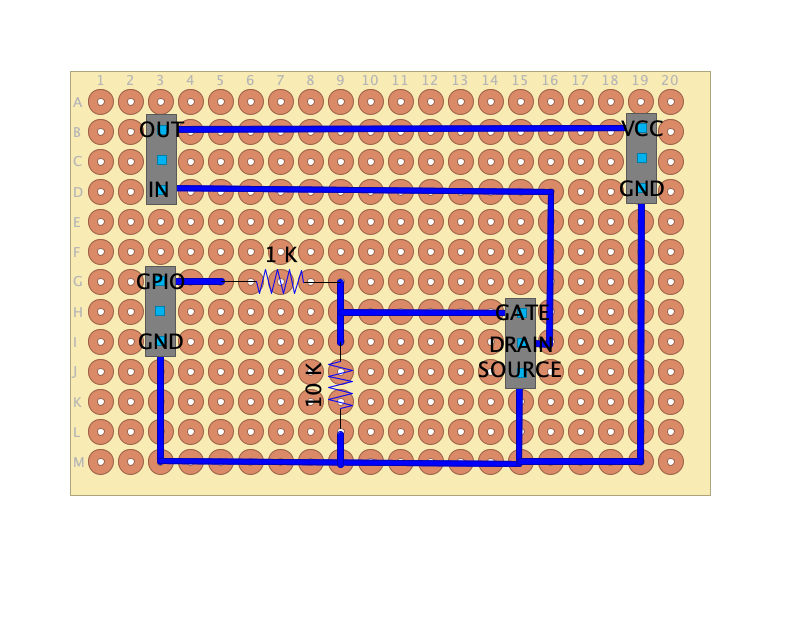
\includegraphics[width=2.6719in,keepaspectratio]{./imagenes/image55.png}

El MOSFET actúa como un interruptor controlado por voltaje. Cuando el voltaje entre gate y source es nulo, no existe camino de conducción entre drain y source y el filamento no recibe corriente. Cuando dicho voltaje supera el umbral del dispositivo que es de entre 1,0 V y 2,0 V, se forma un canal que une drain y source con muy baja resistencia, cerrando el circuito del filamento.

El gate del MOSFET se conecta a un pin GPIO de la Raspberry Pi a través de una resistencia serie de 1 kΩ. Dado que el gate se comporta como un capacitor, cada conmutación del GPIO produciría un pico de corriente elevado para cargarlo o descargarlo. Esta resistencia limita dicho pico a aproximadamente 3,3 mA, valor inferior a la corriente que puede entregar un pin GPIO, protegiendo así a la Raspberry Pi y amortiguando posibles oscilaciones en la línea del gate. Entre el gate y GND se ubica una resistencia de pull-down de 10 kΩ, cuya función es definir el estado del gate cuando el GPIO no lo está controlando. Cuando el GPIO fuerza 3,3 V, el gate alcanza aproximadamente 3 V según el divisor formado por ambas resistencias, lo que asegura el encendido del MOSFET con un consumo en el pin de apenas 0,3 mA. En operación normal el GPIO permanece en nivel bajo y el filamento no conduce corriente. Cuando el software de vuelo determina que debe realizarse el corte, pone el GPIO en nivel alto. El MOSFET pasa a conducir y cierra el circuito batería--filamento--drain--source--GND. La corriente calienta el filamento hasta fundir la cuerda, liberando la carga útil.

\subsection{Comunicación post-aterrizaje}\label{sistema-de-comunicaciuxf3n-post-aterrizaje}

Uno de los objetivos del proyecto es volver a encontrar el dispositivo para lograr obtener todos los datos guardados localmente además de en un futuro poder reutilizarlo. Para ello se decidió utilizar NB-IoT. Se necesita que el dispositivo envíe paquetes de datos muy pequeños. Solo necesitamos que nos envíe las coordenadas GPS para poder encontrarlo. Por eso esta tecnología es la ideal. Además, el canal angosto permite chips de radio más simples, reduce el consumo energético, y permite que la señal recorra distancias más largas o penetre lugares que otros canales no podrían.

Es altamente probable que el dispositivo aterrice en una zona rural muy lejos de una ciudad. Esta tecnología permite igualmente poder tener conectividad a través de la red de Antel. Vamos a aprovechar la altura que va a tener el dispositivo e intentar conectarse a la red antes de tocar la superficie. La línea de vista es mejor en el aire que ya estando en la tierra. Por eso la idea es que cuando esté descendiendo y alcance una altura de alrededor de los 500 metros ya esté mandando datos. A esa altura hay línea de vista directa con varias torres de Antel, sin montes, valles, ni obstáculos. También va a tener tiempo suficiente para enviar varios mensajes antes de tocar el suelo.

\textbf{Fase 1: Descenso (\textgreater1000 m)}

Durante el descenso, el dispositivo va a seguir en modo silencio total para conservar la batería. El GPS va a estar corriendo para ir calculando la posición, pero no transmite nada el módulo de NB-IoT. Solo se transmite la telemetría a través de LoRa.

\textbf{Fase 2: Trigger de altitud (1000 m)}

El altímetro detecta que se cruza el umbral de 1000 m sobre el nivel del suelo. En ese momento:

\begin{enumerate}
\def\labelenumi{\arabic{enumi}.}
\item
  Se activa el módulo NB-IoT Quectel BC660K-GL
\item
  El GPS toma un fix de posición
\item
  Se envían ráfagas repetidas de mensajes con coordenadas GPS, altitud y estado de batería cada 2 minutos.
\item
  El dispositivo tiene visión despejada de las antenas celulares.
\item
  Cuando se confirma la transmisión a través de NB-IoT, se apaga la transmisión por LoRa para consumir menos energía.
\end{enumerate}

Decidimos activar el módulo NB-IoT a los 1000 metros, ya que demora tiempo (entre 5 y 30 segundos dependiendo de la cobertura) el proceso de conexión. Por lo tanto, va a tener tiempo de conectarse a la red mientras todavía tiene buena visibilidad, y ya estará listo y conectado cuando pase por los 500 m enviando datos. La ventaja de empezar la conexión antes es que si la primera torre no responde, va a tener tiempo de reintentar con otra antes de quedar en el suelo.

\textbf{Fase 3: Post-aterrizaje (superficie)}

Después de llegar a tierra, el dispositivo continúa enviando cada 10 minutos hasta recuperarlo o se agote la batería. Puede llegar a pasar que continúe cambiando su ubicación si alguien o algo lo mueve. Por lo tanto es necesario seguir recibiendo la ubicación hasta encontrarlo. Gracias al buen link budget de NB-IoT, aunque quede en un monte o en un valle, hay muchas chances de obtener señal.

\subsection{Procedimiento de localización y recuperación}\label{localizacion-recuperacion}

\pendiente{Procedimiento de localización y recuperación.}

\parte{Parte V: Segmento terrestre}

\section{Estación terrena}\label{arquitectura-recepciuxf3n-de-telemetruxeda-y-video}


Según \cite{ref40} el sistema de recepción se compone de la antena, seguido de otros componentes como amplificadores, diplexores, atenuadores, entre otros. Finalizando con un filtro pasa banda, seguido de un LNA y por último el receptor.

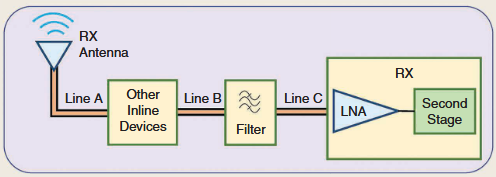
\includegraphics[width=5.1667in,keepaspectratio]{./imagenes/image7.png}

La arquitectura que se utilizará es la siguiente:

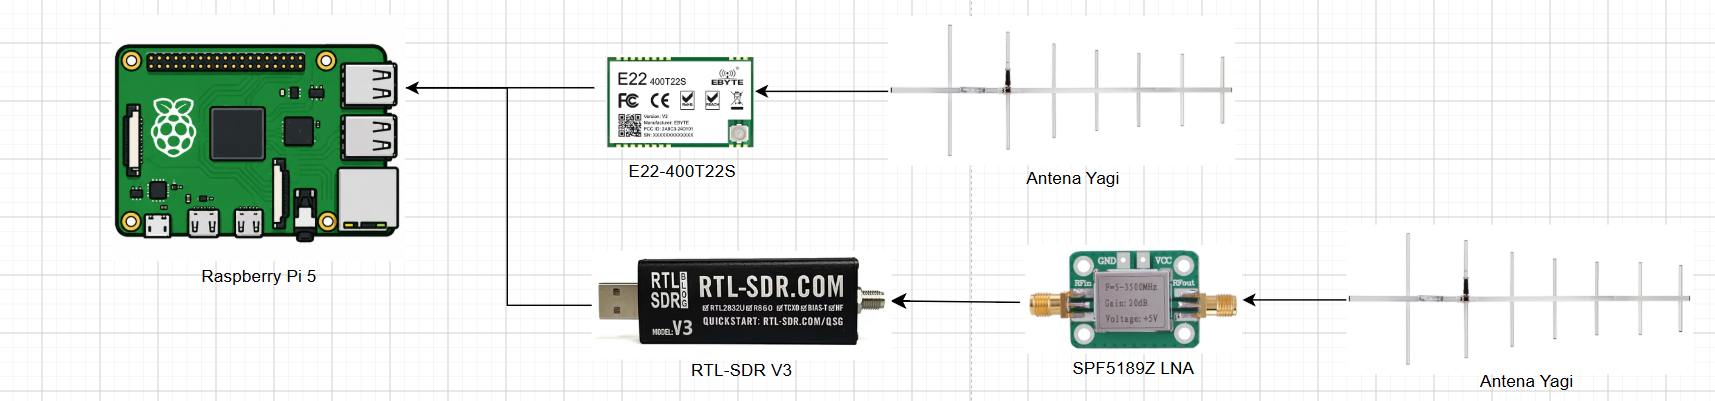
\includegraphics[width=\linewidth,keepaspectratio]{./imagenes/image36.png}

AGREGAR FILTRO

\subsection{Arquitectura general}\label{estaciuxf3n-terrena}

Para construir la estación terrena se seleccionaron materiales económicos. Se adquirieron tubos de PVC, conexiones de tubo en forma de T y L, tornillos para fijar las conexiones, y planchas de madera para la base. Adicionalmente, se construyó para que se pueda modificar el tilt y azimut manualmente.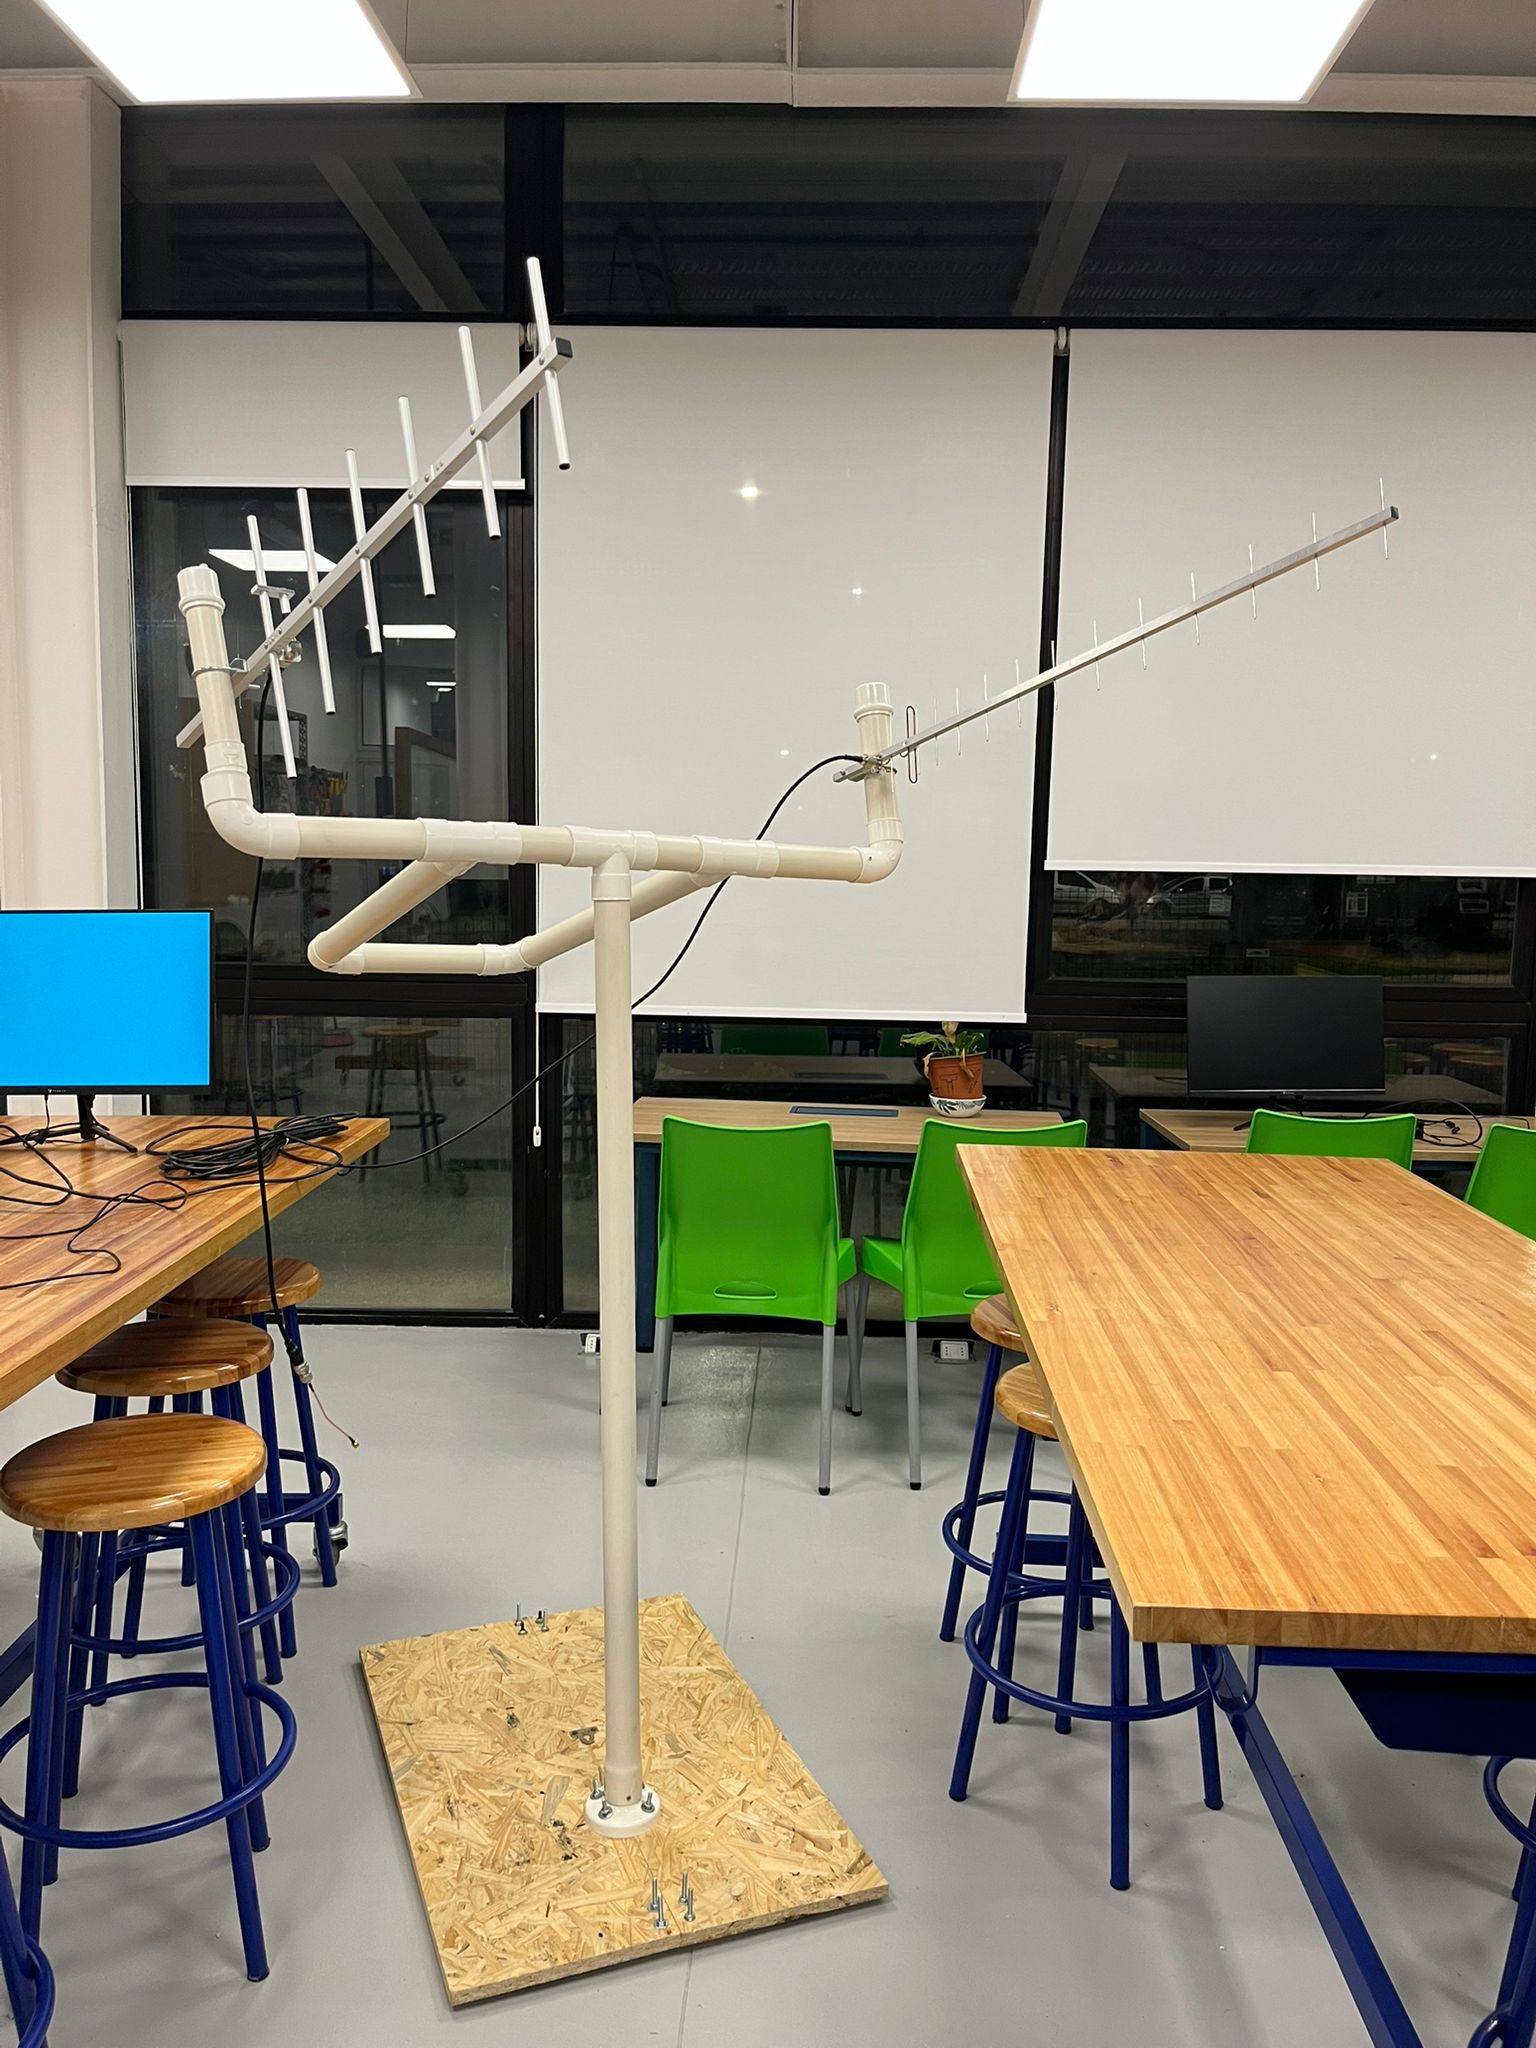
\includegraphics[width=2.5573in,keepaspectratio]{./imagenes/image37.png}

Para el hardware, se compró una caja de electricidad y se adaptó para fijar cada componente. El módulo LoRa, las luces LED, y el LNA, se soldaron sobre una placa.

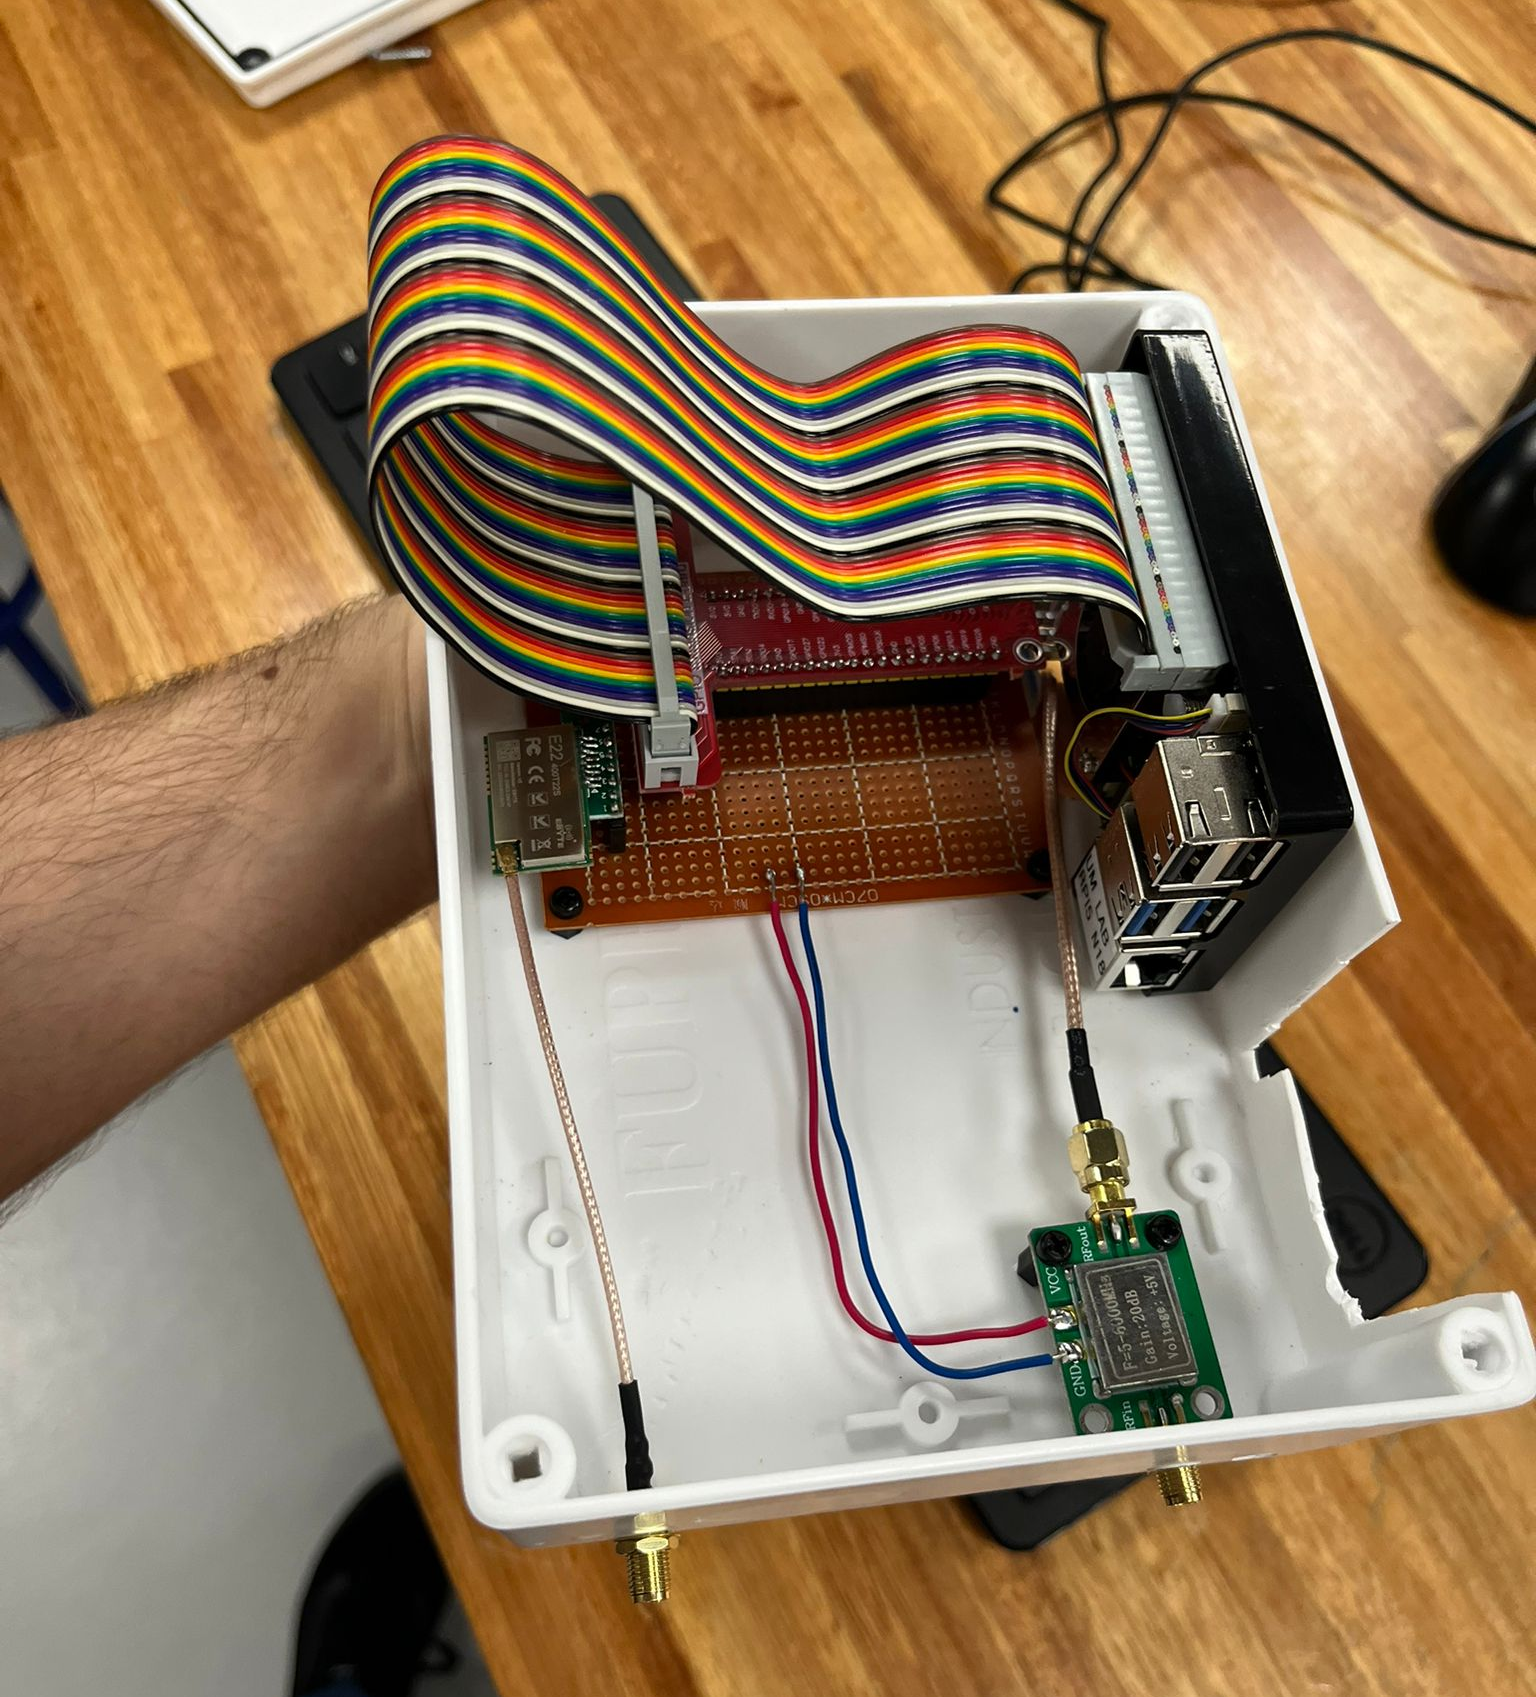
\includegraphics[width=1.7135in,keepaspectratio]{./imagenes/image92.png}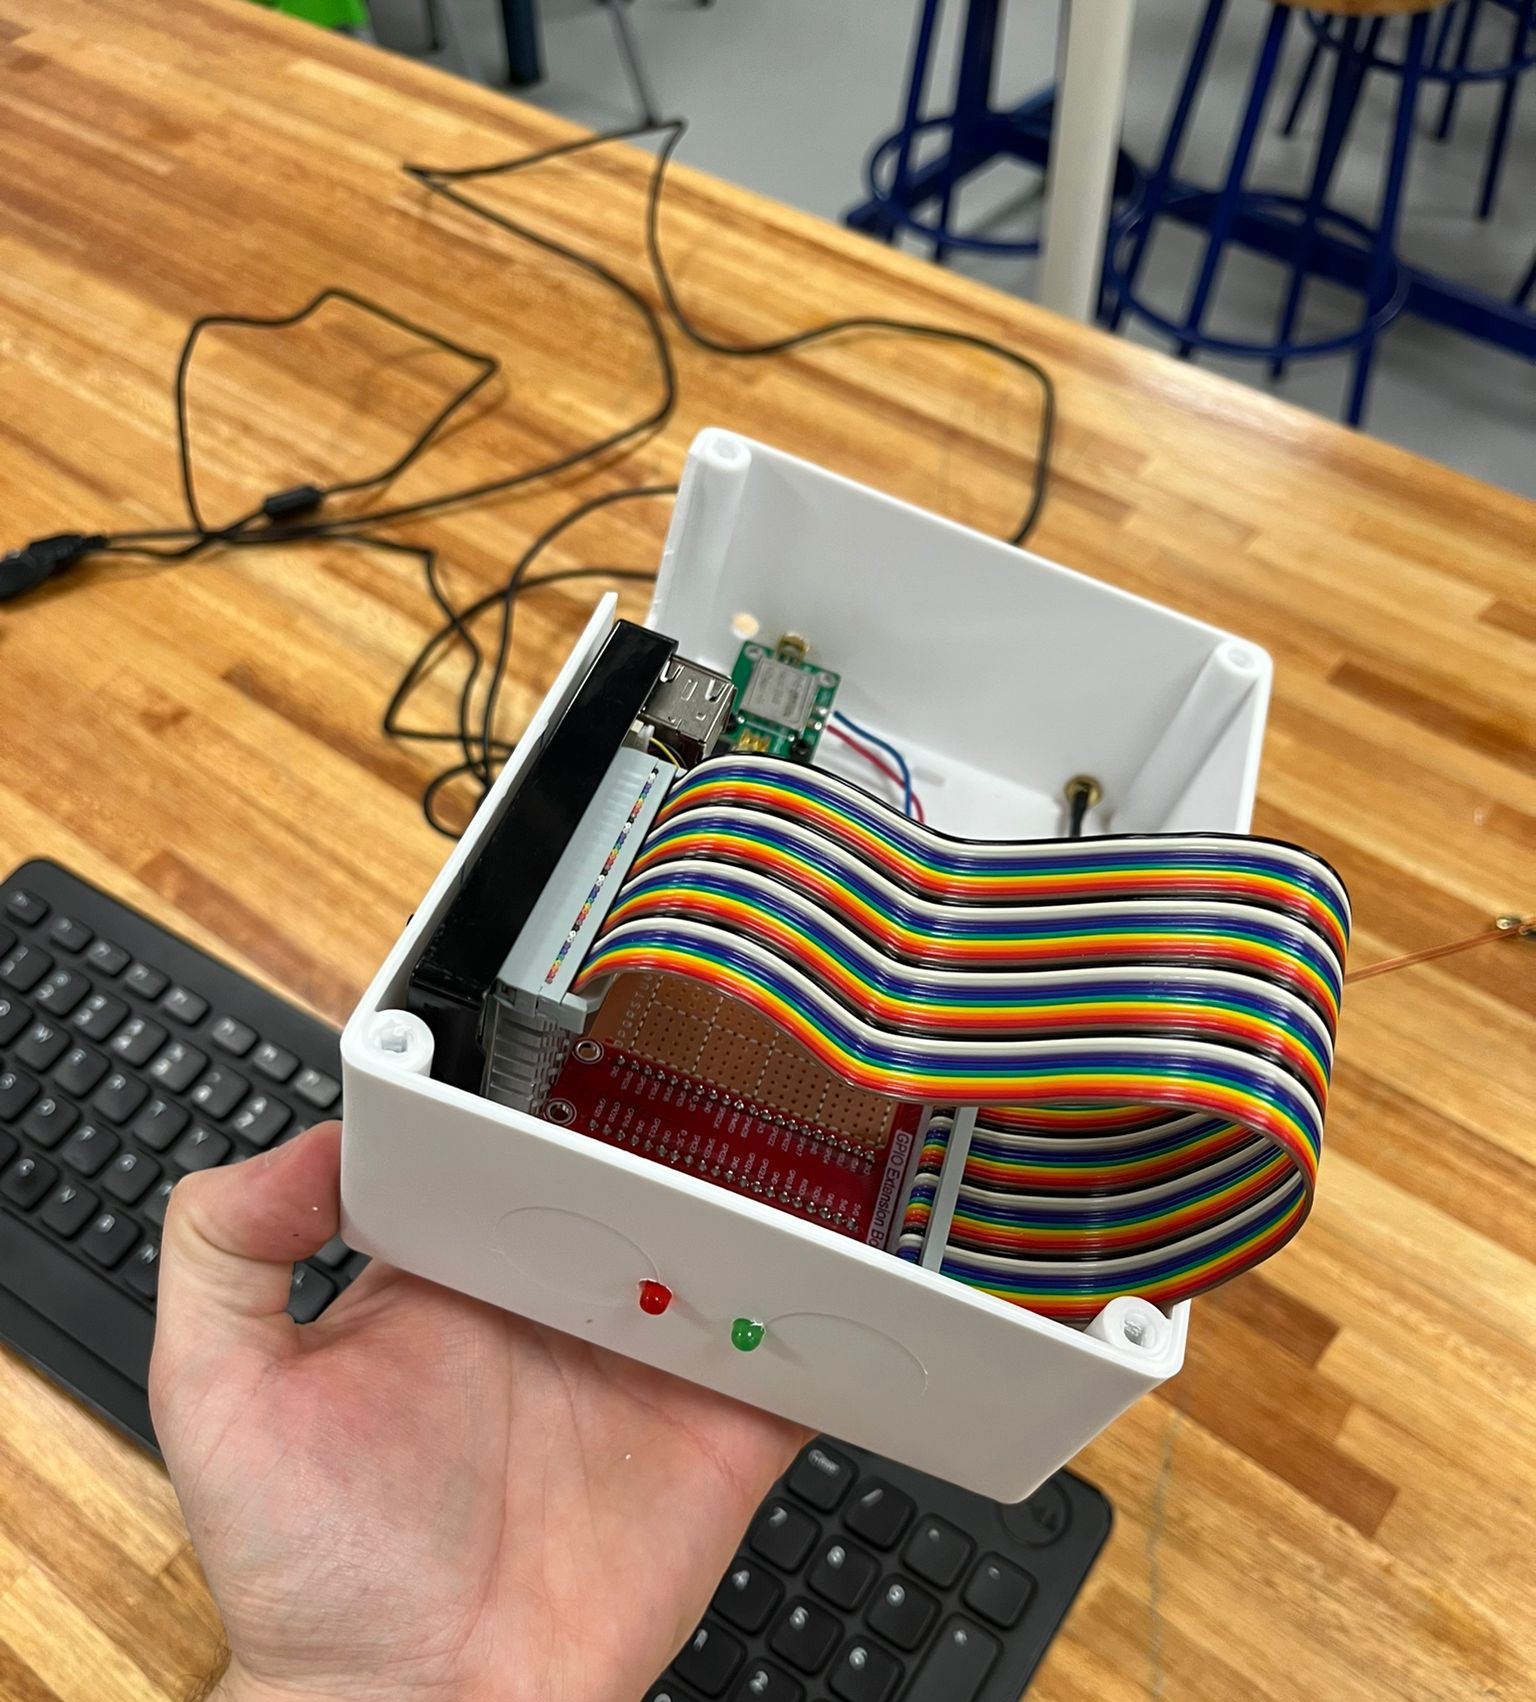
\includegraphics[width=1.7116in,keepaspectratio]{./imagenes/image10.png}

Una vez todo fijo a la caja, se colocó en la estructura de la estación terrena y se verificó su correcto funcionamiento.

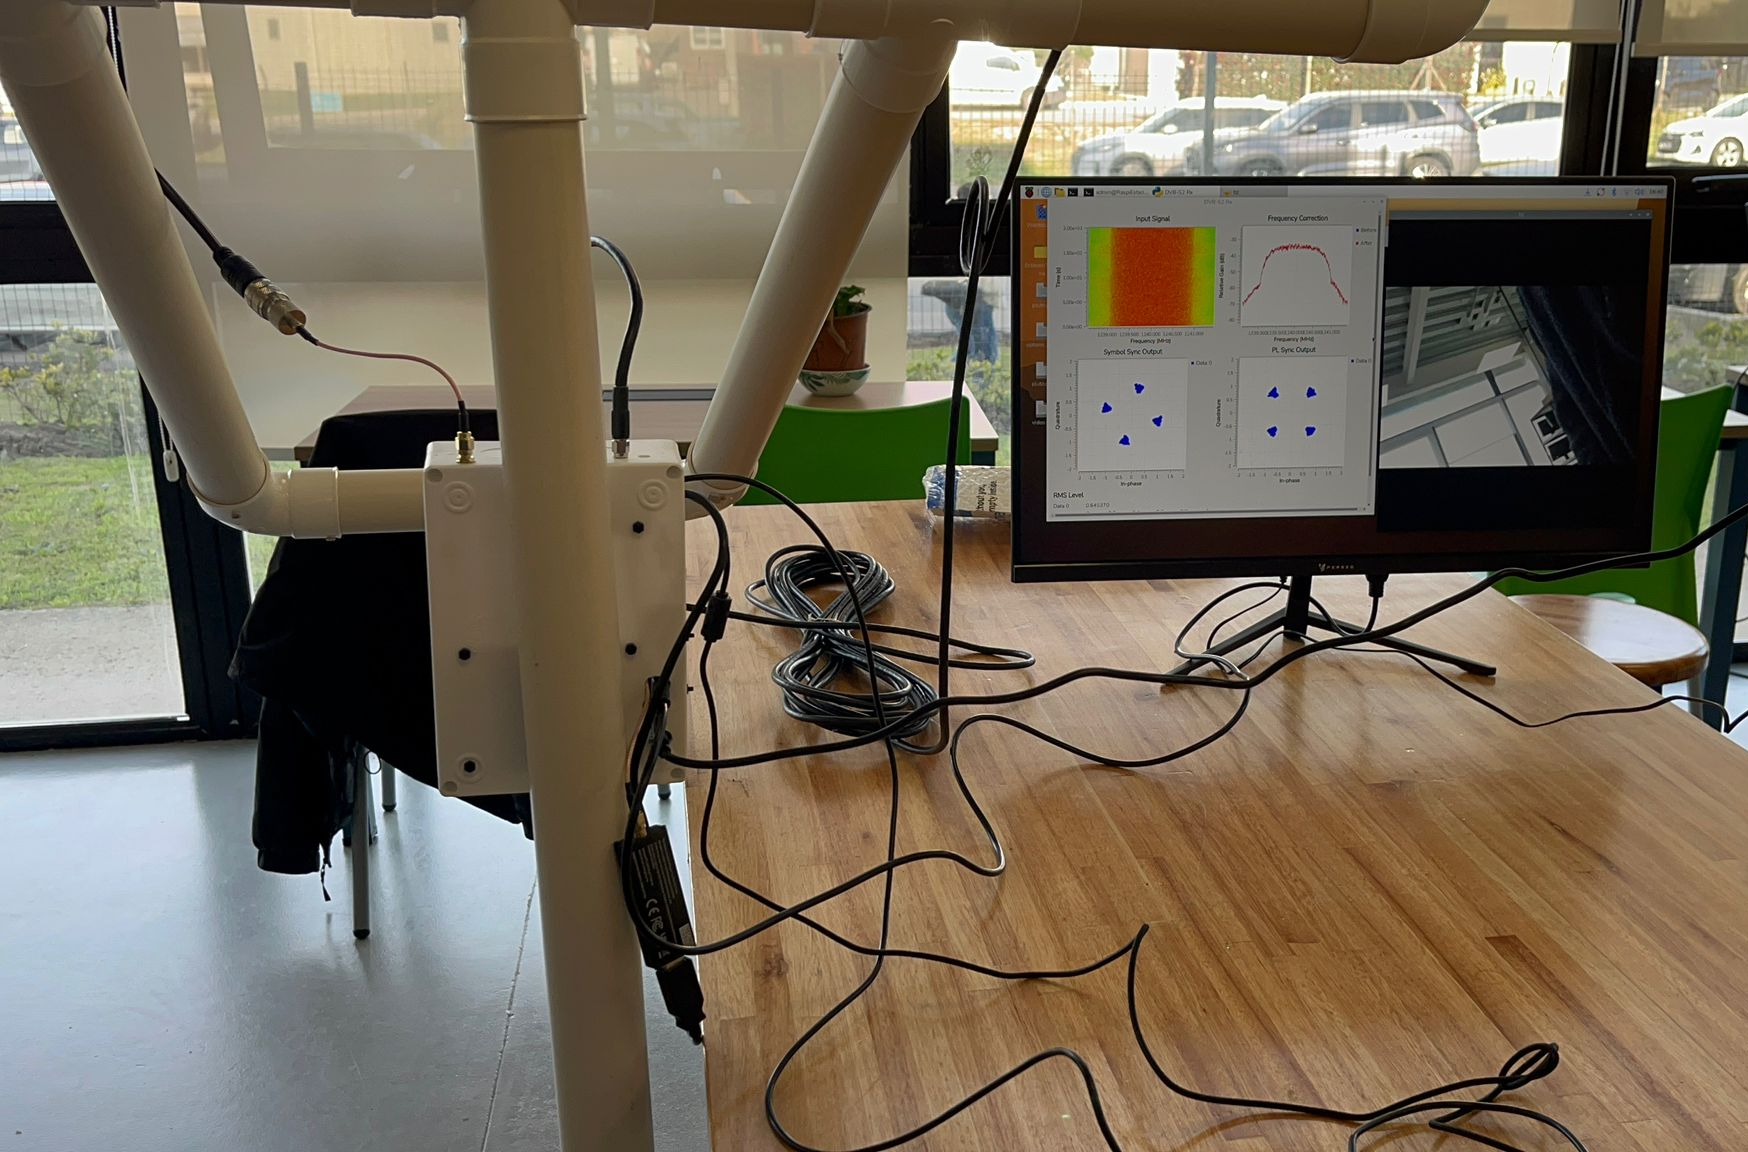
\includegraphics[width=4.2500in,keepaspectratio]{./imagenes/image11.png}

\subsection{Antenas de recepción}\label{antenas-recepciuxf3n-de-video-y-telemetruxeda}

En la estación terrena, se determinó que la mejor opción es tener una antena de ganancia media o alta. Las antenas Yagi-Uda son muy utilizadas en proyectos similares \cite{ref2,ref44,ref71}. La estación terrena se encuentra en un lugar fijo y estable en la Tierra. A diferencia del globo, que está en movimiento constante y girando, la antena de la estación terrena no necesita ser omnidireccional. Esto permite utilizar antenas altamente directivas que concentran su sensibilidad en una dirección específica, captando señales mucho más débiles. De esta forma, compensar la baja ganancia y la radiación débil del transmisor del globo, logrando un buen enlace aunque la antena del globo sea simple y de baja ganancia.

La antena Yagi-Uda se trata de un arreglo parasitario, lo que significa que solo un elemento está conectado directamente al transmisor, mientras que los demás (parásitos) reirradian energía inducida por el campo electromagnético del primero. Se compone por tres elementos: reflector, excitado y director. El elemento excitado es típicamente un dipolo plegado. El reflector se coloca detrás del elemento excitado, en dirección opuesta a la radiación deseada, permitiendo cancelar o reducir la señal hacia atrás. Suele ser 3\% más largo que la longitud de media onda en el conductor. Los elementos directores se colocan delante del elemento excitado en la dirección de máxima radiación. El primer director es típicamente un 3\% más corto que el elemento excitado. Al añadir más directores, se incrementa la ganancia y se estrecha el haz de la señal \cite{ref70}. 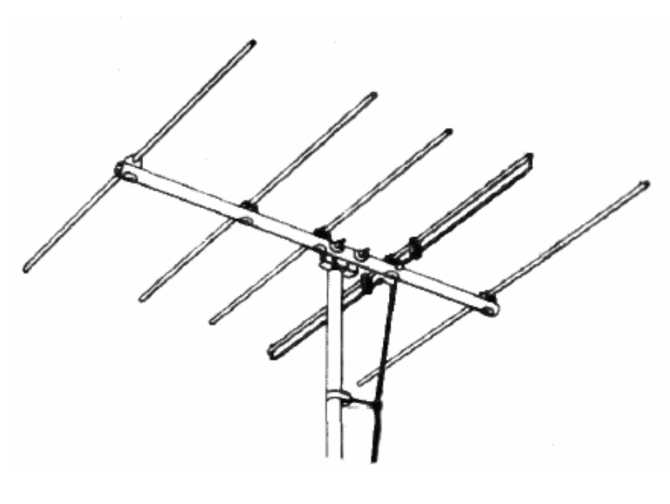
\includegraphics[width=2.5938in,keepaspectratio]{./imagenes/image20.png}

Los elementos se montan paralelos entre sí sobre un botalón (boom). El espaciamiento típico varía entre 0.1λ y 0.25λ. Un espaciamiento mayor suele mejorar el ancho de banda y la ganancia, pero requiere un boom más largo. La impedancia de una antena Yagi es mucho más baja que la de un dipolo común debido a la fuerte interacción eléctrica con sus elementos parásitos (reflector y directores) \cite{ref70}.

\subsubsection{Antenas adquiridas}\label{antenas-adquiridas}

Se verificó el acoplamiento de las antenas Yagi adquiridas.

Telemetria:

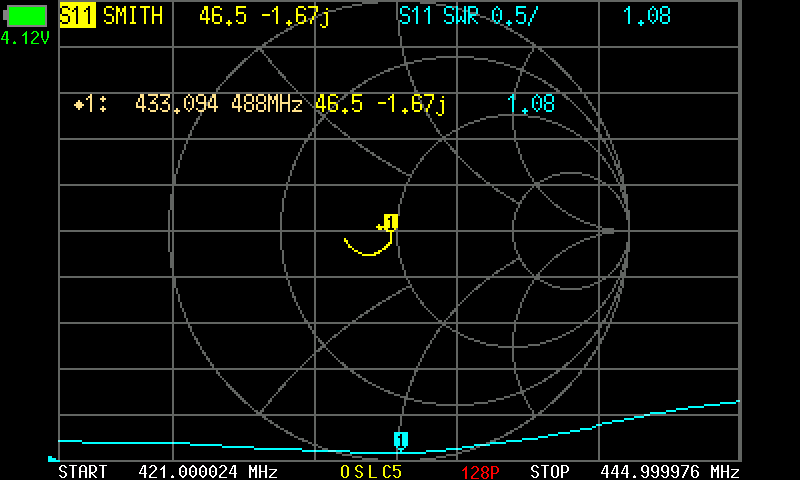
\includegraphics[width=\linewidth,keepaspectratio]{./imagenes/image12.png}

Video:

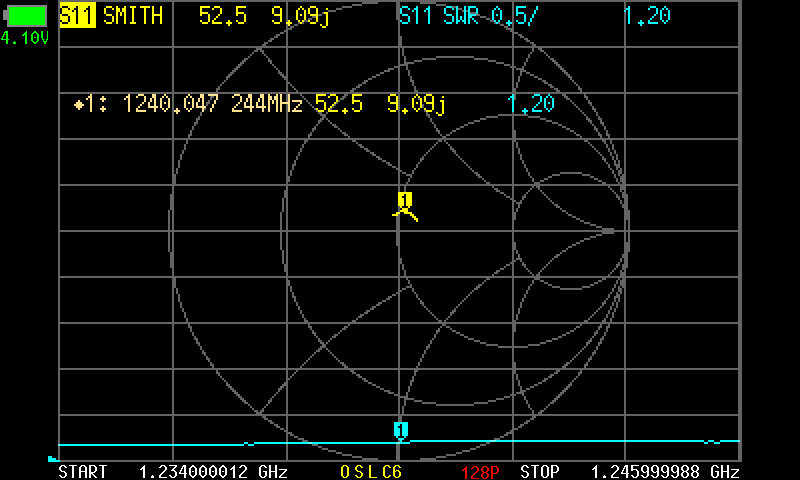
\includegraphics[width=\linewidth,keepaspectratio]{./imagenes/image2.png}

Las dos antenas obtuvieron muy buenos acoplamientos, ambas reflejan menos del 1\% de la potencia que les incide.

\subsection{LNA y filtro pasa banda}\label{lna-filtro}
\subsubsection{Amplificador de bajo ruido}\label{amplificador-de-bajo-ruido-1}

El RTL-SDR tiene un piso de ruido típico entre 3 - 4 dB \cite{ref63}. Se adquiere el LNA SPF5189Z diseñado para operar entre 50MHz y 4000MHz. En 1240 mhz, el piso de ruido es de entre 0.6 (25°C) y 0.8 dB (85°C). La ganancia es ligeramente superior a 16 dB, dependiendo de la temperatura, y tiene una P1dB de 22.5 dBm \cite{ref64}.

El efecto que tiene el LNA es el siguiente:

\(T_{R}\  = \ T_{LNA} + \frac{T_{segunda\ etapa}}{G_{LNA}}\) \cite{ref40} Es decir, la temperatura de ruido se reduce según la ganancia del LNA. En este caso, el piso de ruido final queda en:

\(T_{R}\  = \ 0.7 + \frac{4}{16}\  = \ 0.95\ dB\)

\subsubsection{Filtro pasa banda}\label{filtro-pasa-banda}
Para rechazar interferencias fuera de banda, evitar saturación e intermodulación, y limitar el ruido. Se adquirió el filtro pasabanda ZX75BP-1205-S+ de MiniCircuits:
\begin{itemize}
    \item Banda: 1155 -1255 Mhz
    \item Máxima potencia de entrada: 10 W
    \item Impedancia: 50 ohm
\end{itemize}

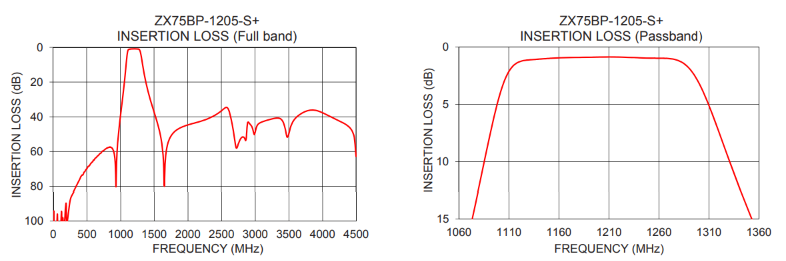
\includegraphics[width=\linewidth,keepaspectratio]{./imagenes/respuesta-filtro.png}


\subsection{Receptor y demodulación}\label{receptor-cap}
\subsubsection{Receptor}\label{receptor}

Para recibir el video, se evaluaron varias opciones. \cite{ref49} compara distintos tipos de SDR, de distinto precio, frecuencias de operación y resolución de ADC.

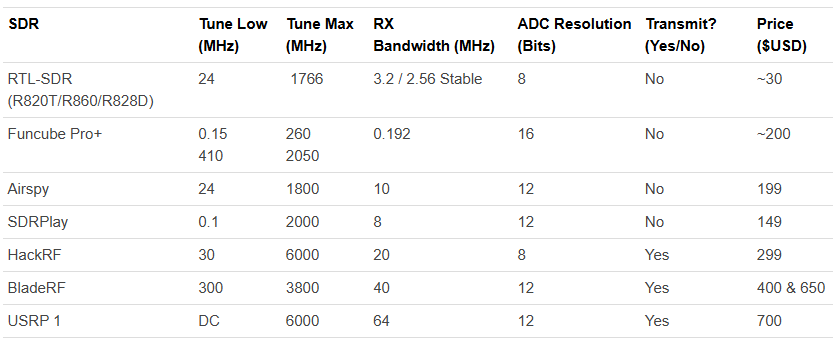
\includegraphics[width=\linewidth,keepaspectratio]{./imagenes/image5.png}

\cite{ref43} \hl{destaca al RTL-SDR como un receptor de ultra bajo costo que es ideal para el análisis espectral básico, muy utilizado en proyectos de globos para recibir telemetría y datos de GPS.}

\hl{El RTL-SDR ha sido utilizado como receptor de video digital en diversos proyectos experimentales. El proyecto OH3VHH-1 recibió transmisiones DVB-S1 desde un globo estratosférico} \cite{ref51}\hl{, el Horus Project empleó RTL-SDR para la recepción de DATV de gran altitud} \cite{ref52}\hl{, y radioaficionados utilizaron este mismo dispositivo para recibir las transmisiones DVB-S de la Estación Espacial Internacional (ISS)} \cite{ref53}\hl{.}

\hl{Se adquirió un RTL-SDR V3 por su muy bajo costo comparado con las otras opciones. Además, su ancho de banda de operación estable de 2.56 Mhz es ideal para lo que requerimos para el video. También cuenta con una comunidad muy amplia y mucha documentación disponible.}

El receptor de telemetría es el mismo módulo \hl{EBYTE LoRa E22-400T22S.}

\subsubsection{Librería gr-dvbs2rx}\label{libreria-gr-dvbs2rx}

Para resolver la transmisión en DVB-S2, se utilizará la librería gr-dvbs2rx. Es un módulo de GNU Radio externo con implementaciones completas de transmisor y receptor DVB-S2 para radio definida por software (SDR). Incluye una biblioteca compartida con los bloques esenciales (PL, FEC, BBFRAME) de procesamiento de señales para procesar las muestras IQ de entrada y recuperar un flujo de transporte MPEG (TS) en la salida \cite{ref66}.

Además, proporciona la aplicación dvbs2-tx para la transmisión. Al igual que la aplicación de recepción, conecta los bloques de procesamiento de transmisión. Las aplicaciones de transmisión y recepción son altamente personalizables mediante las opciones de línea de comandos y admiten el uso de dispositivos SDR (RTL-SDR, USRP, PlutoSDR y BladeRF) como interfaces de entrada/salida \cite{ref66}.

\section{Dashboard}\label{dashboard}

\textbf{\hfill\break
}

\parte{Parte VI: Validación y cierre}

\section{Pruebas del sistema}\label{pruebas-de-transmisiuxf3n-de-video-y-telemetruxeda}

\subsection{Métricas de evaluación}\label{muxe9tricas-para-evaluar-calidad-de-video-y-desempeuxf1o-de-los-enlaces.}

\subsection{Pruebas de laboratorio}\label{laboratorio}

En primer lugar, después de varios intentos, se lograron las transmisiones de video y telemetría en el laboratorio, a menos de 10 metros de distancia.

Telemetria: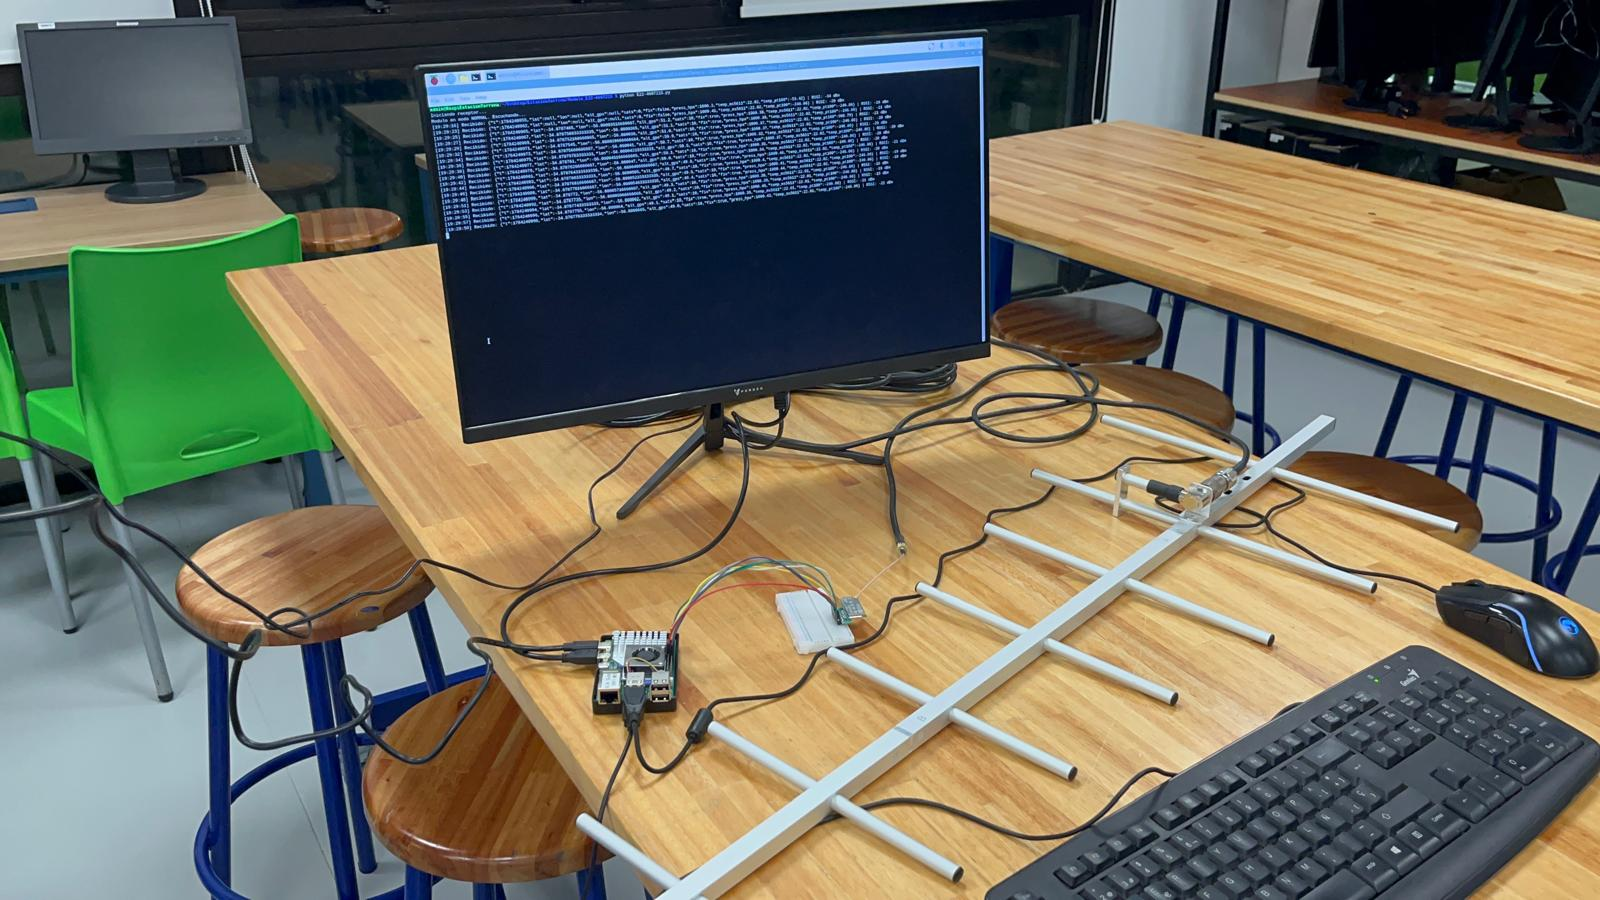
\includegraphics[width=3.0497in,keepaspectratio]{./imagenes/image88.png}

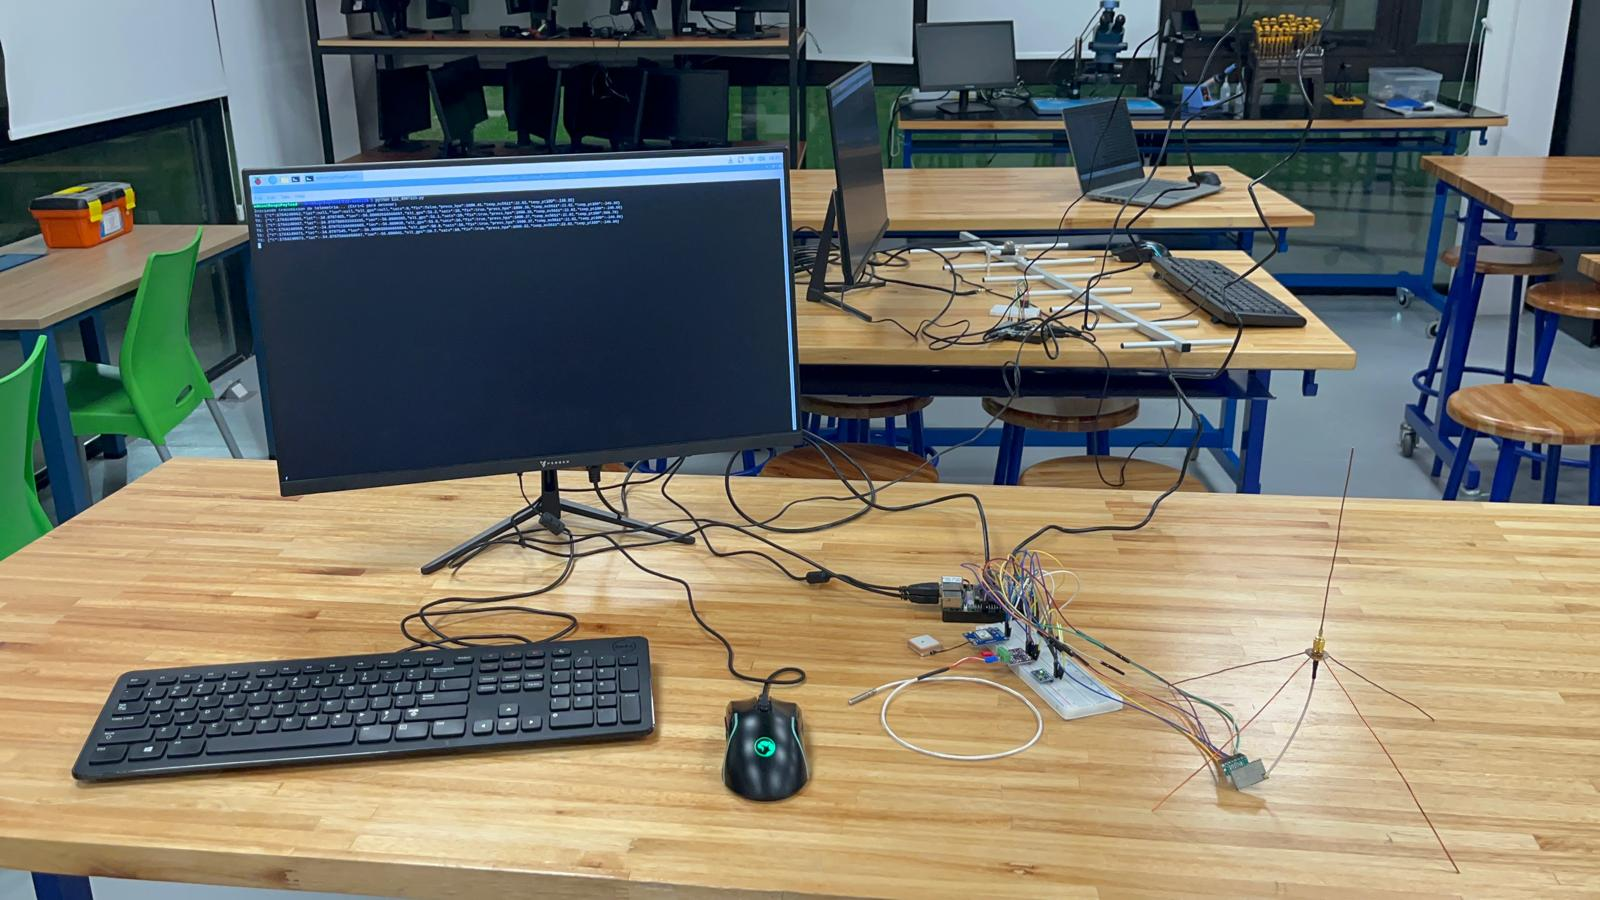
\includegraphics[width=3.0473in,keepaspectratio]{./imagenes/image17.png}

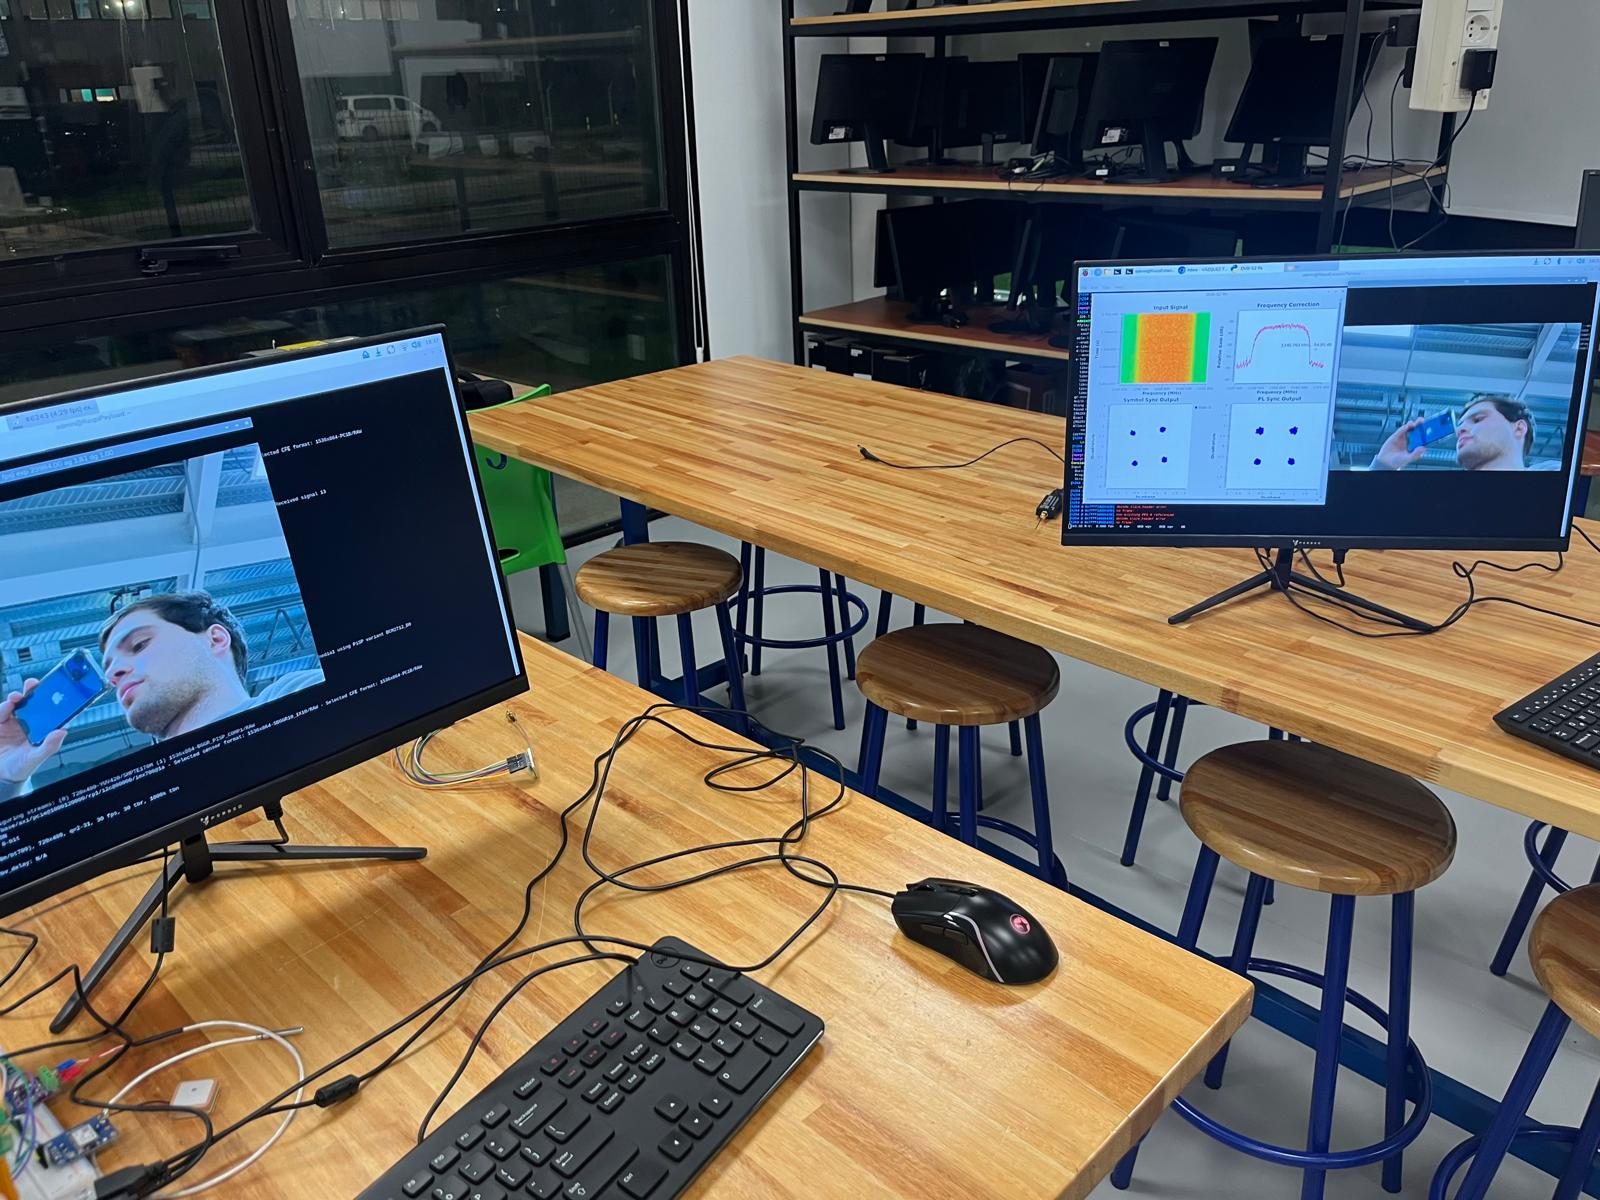
\includegraphics[width=2.7031in,keepaspectratio]{./imagenes/image96.png}

Video:

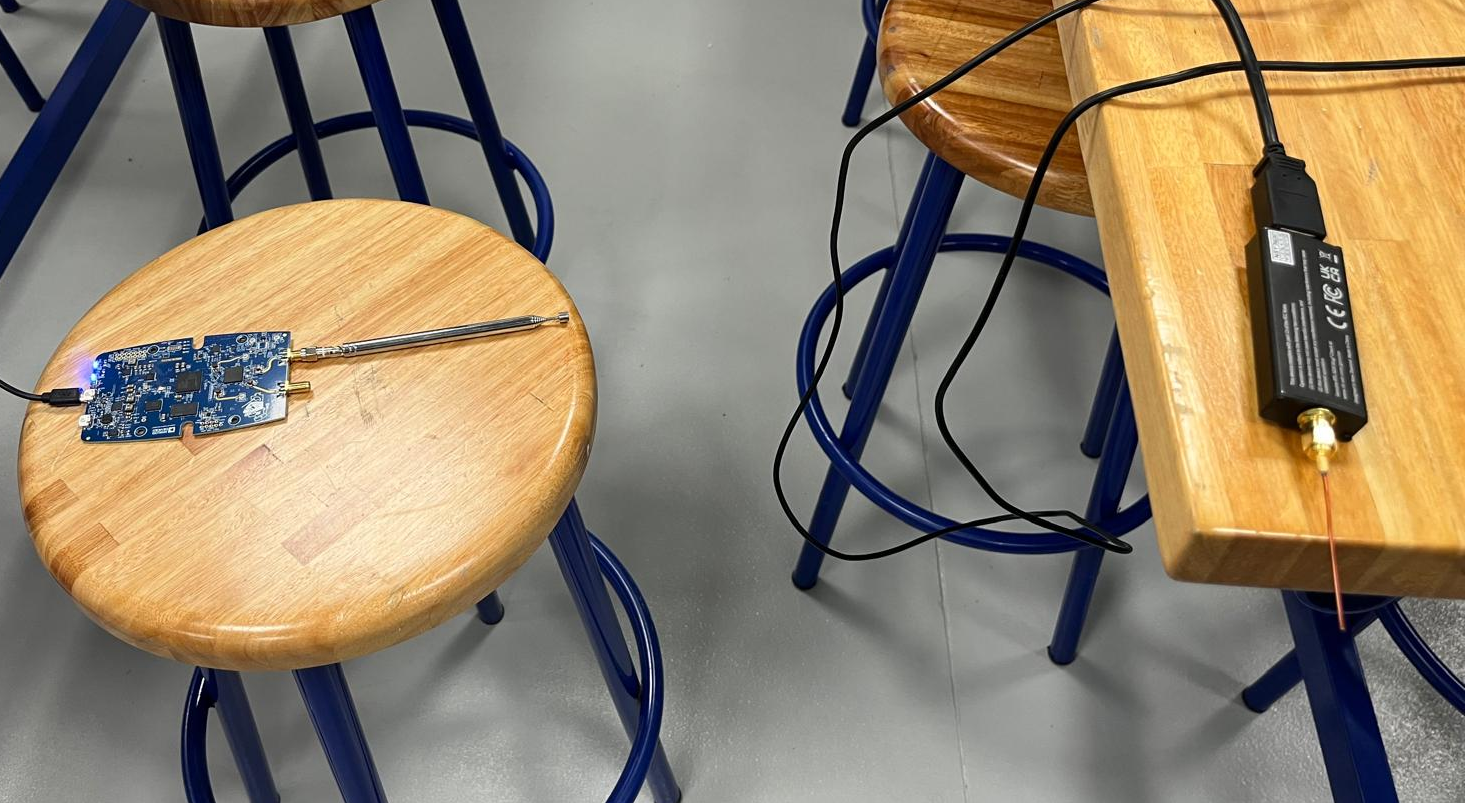
\includegraphics[width=2.9479in,keepaspectratio]{./imagenes/image39.png}

\subsection{Pruebas a corta distancia}\label{corta-distancia}

Después, se verificó el funcionamiento de los enlaces en simultáneo a una distancia de aproximadamente 50 metros. En esta prueba se utilizaron las dos antenas yagi en el lado de la estación terrena, y dos antenas monopolo del lado.

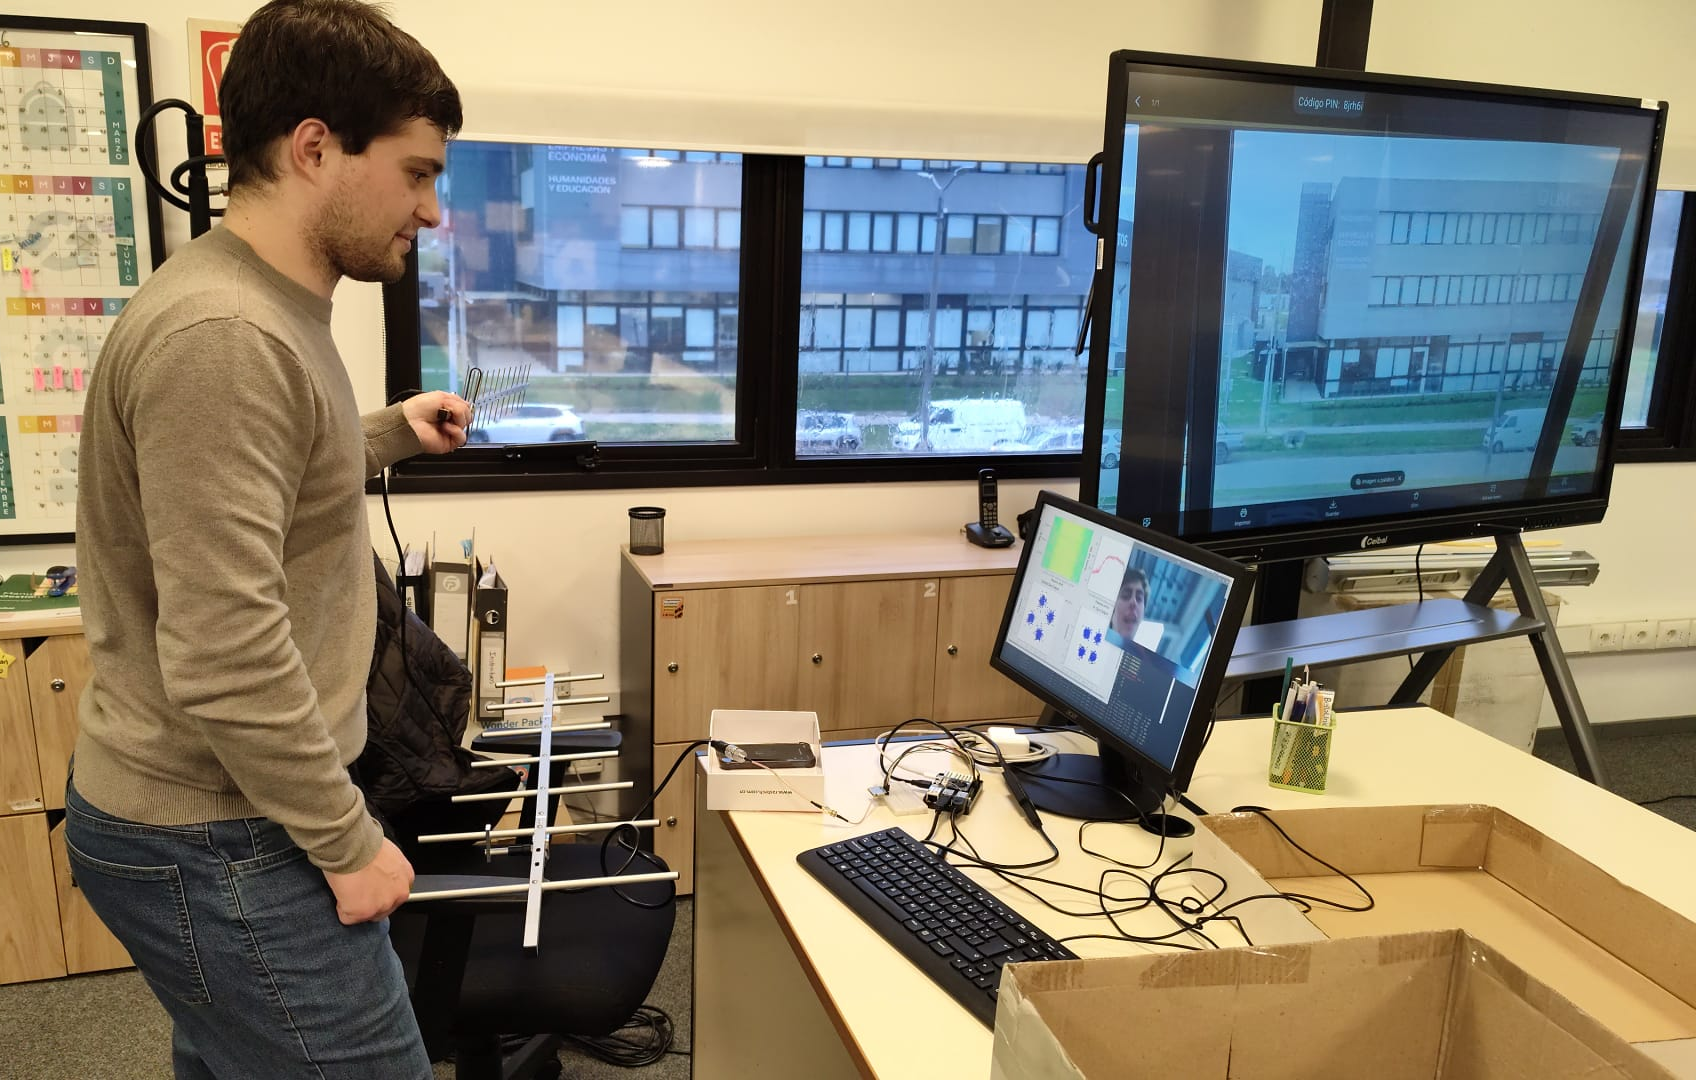
\includegraphics[width=2.7781in,keepaspectratio]{./imagenes/image43.png}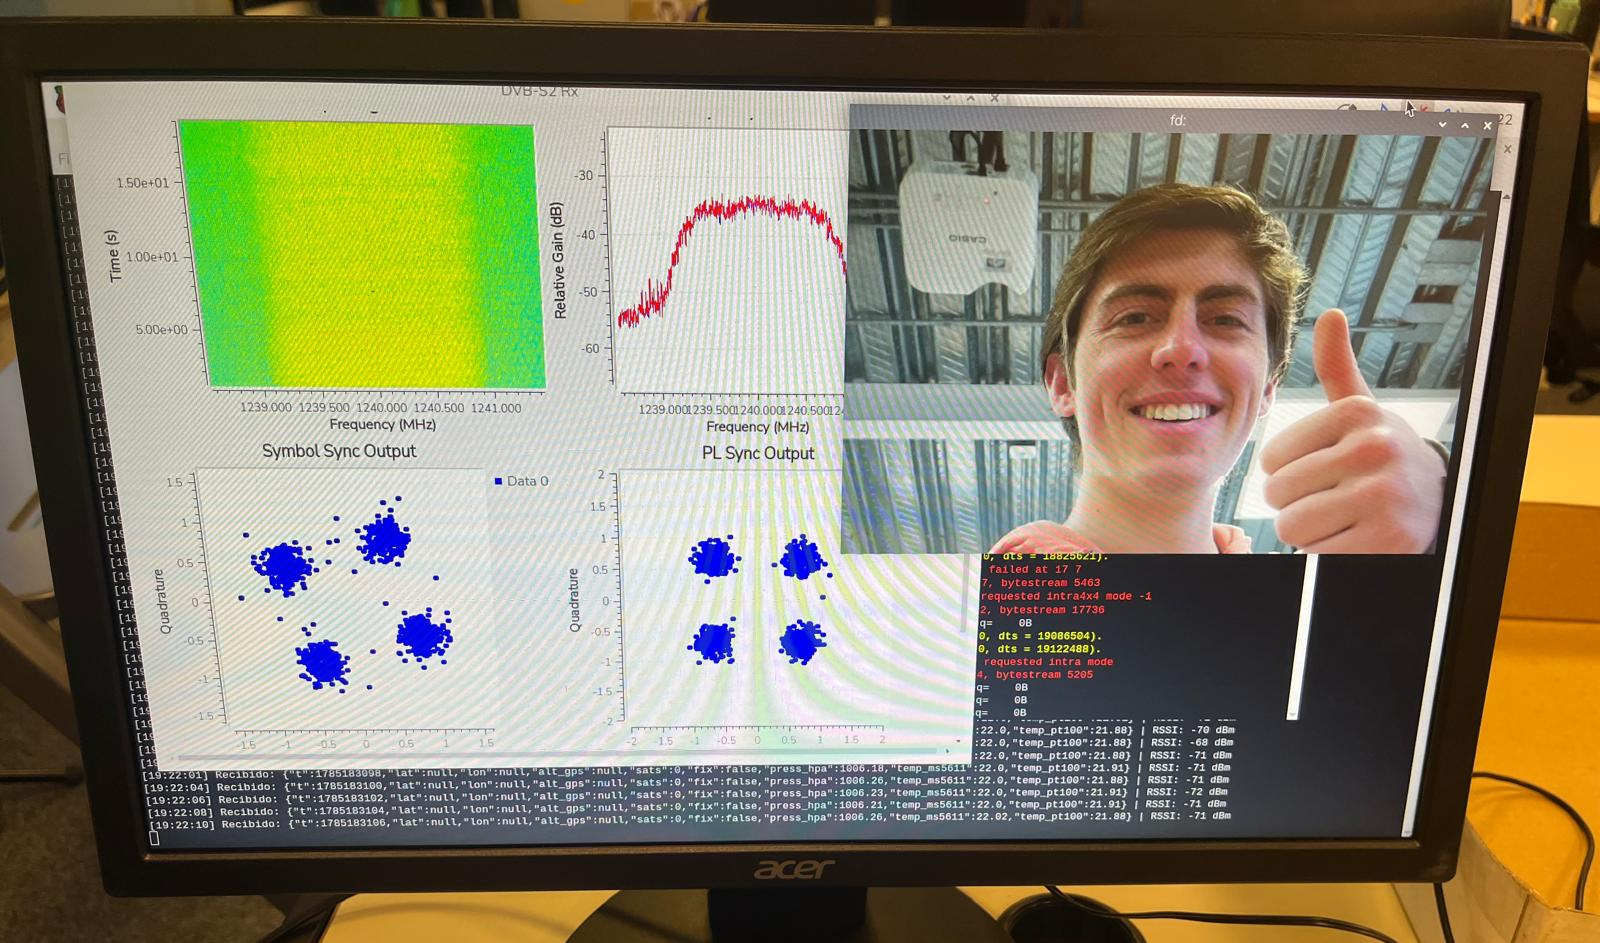
\includegraphics[width=3.0093in,keepaspectratio]{./imagenes/image98.png}

\subsection{Simulación de larga distancia en pasillo}\label{simulaciuxf3n-larga-distancia-en-pasillo-de-la-universidad}

Utilizando un medidor de potencia, se verificó la potencia con la que salía la señal de video. La prueba dio una potencia de entre 0 y 1 dBm. El ADALM-PLUTO SDR tiene una máxima potencia de salida de 7 dBm. Se puede variar la potencia de la señal alterando la escala de las muestras de los símbolos QPSK.

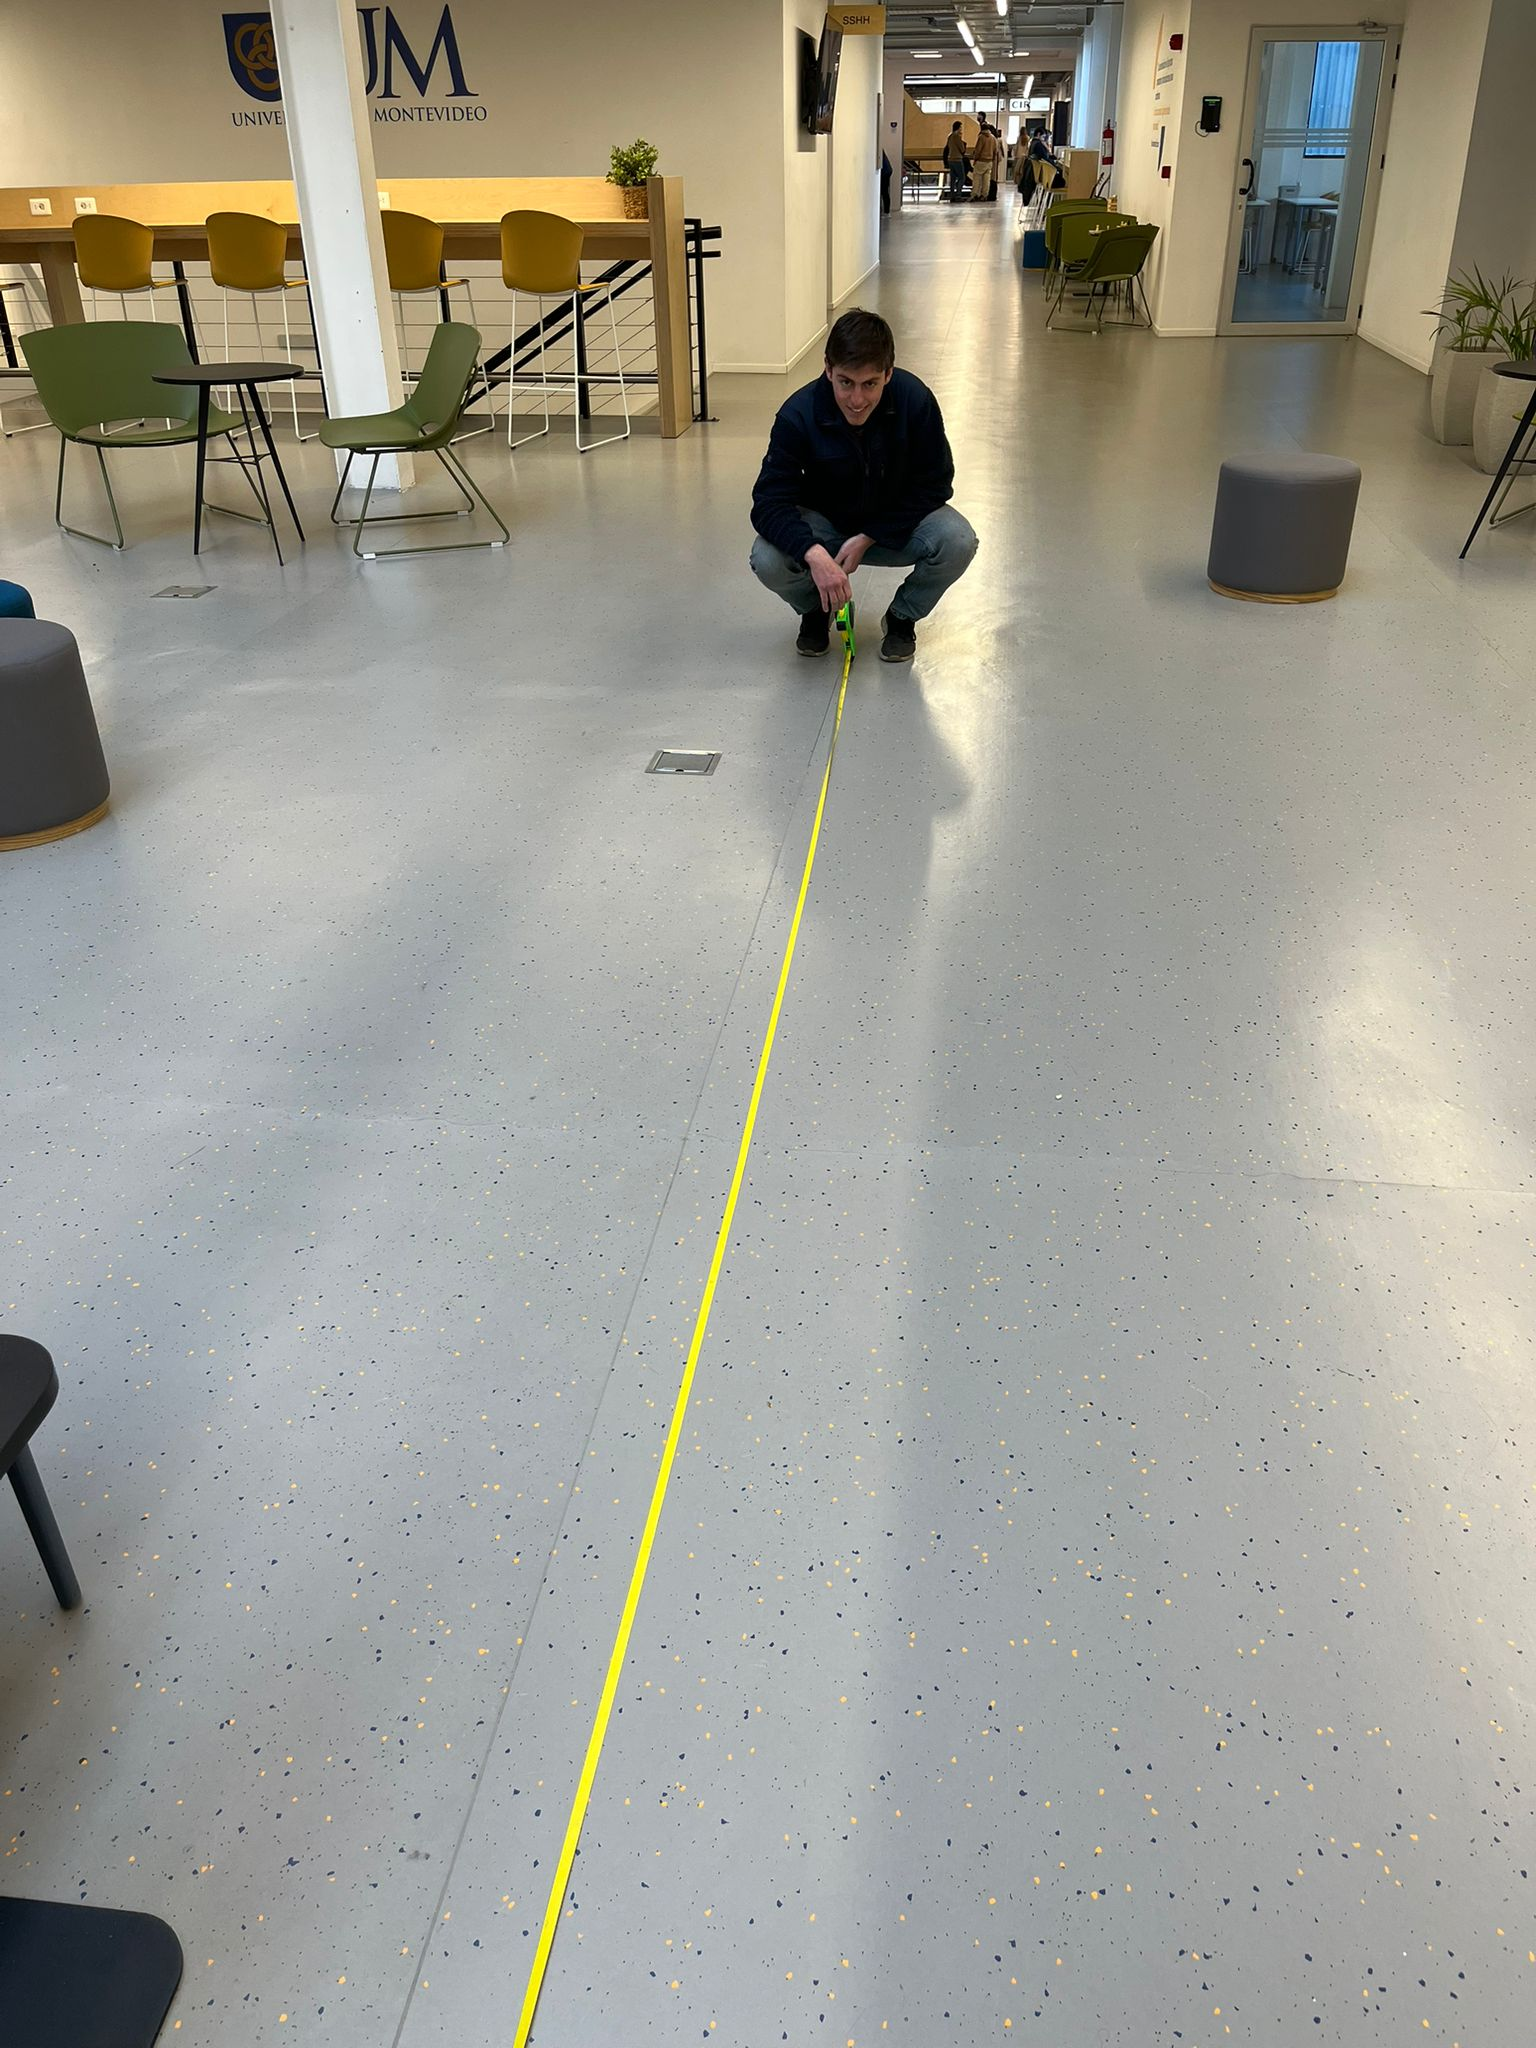
\includegraphics[width=1.7656in,keepaspectratio]{./imagenes/image58.png}

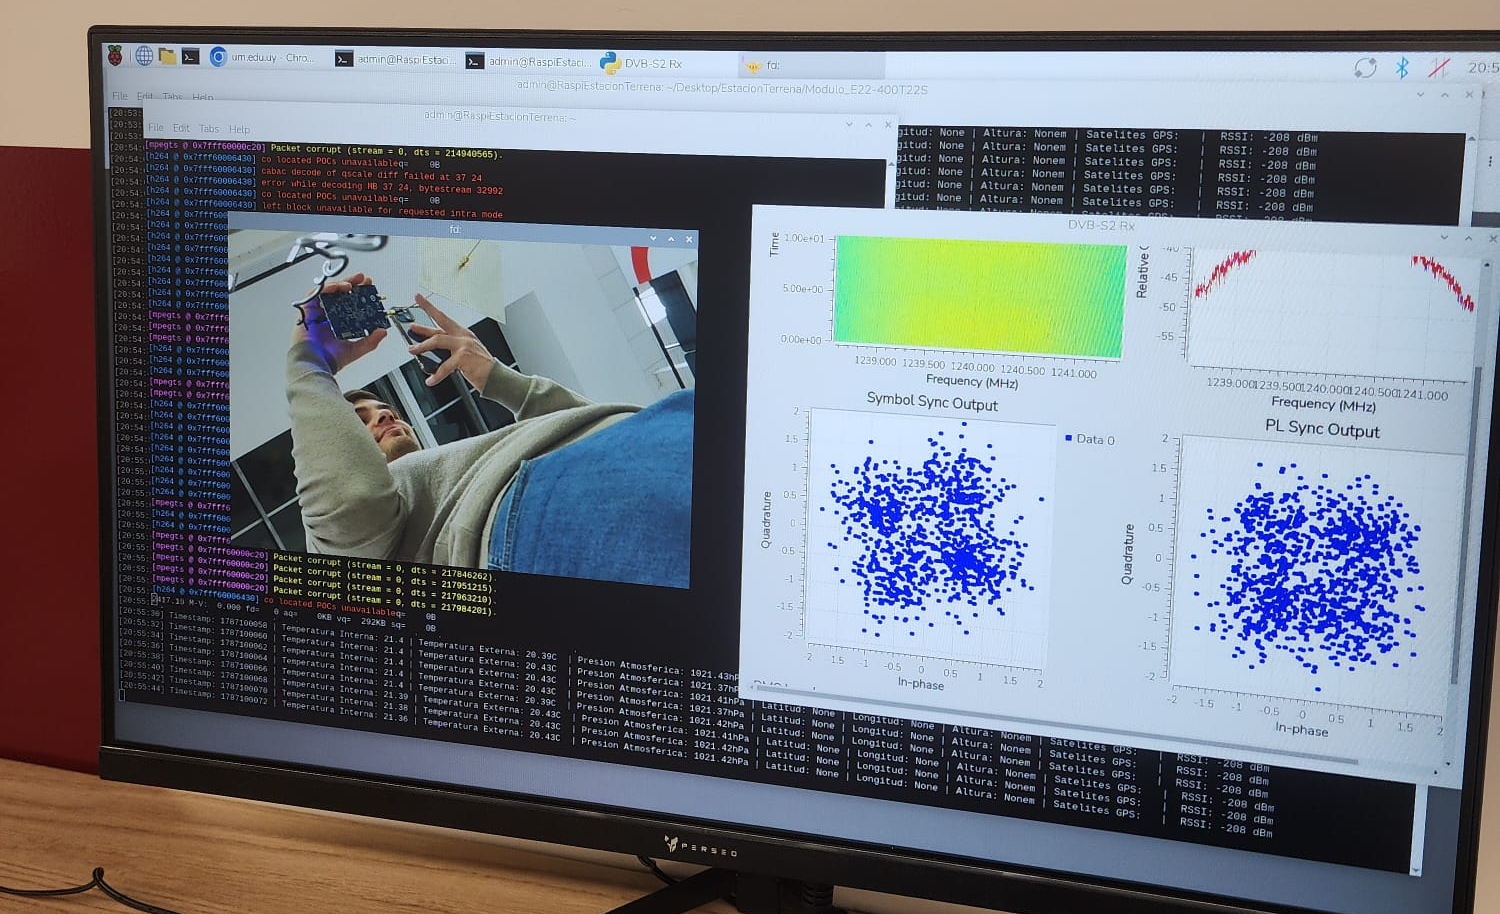
\includegraphics[width=3.7510in,keepaspectratio]{./imagenes/image44.png}

Se realizó una prueba de larga distancia preliminar en el pasillo de la universidad con línea directa. La señal que salía del transmisor tenía una potencia de entre 0 y 1 dBm. Simulando una atenuación inicial de aproximadamente 30 dB. Entre el transmisor y el receptor habían aproximadamente 65 metros, por lo que en 1240 mhz suma 70 dB de atenuación. Del lado del receptor se conectaron atenuadores pasivos entre la antena y el LNA. Se tenía un atenuador de 10 dB y otros dos de 20 dB. Se logró recibir video teniendo una atenuación total de 150 dB, pero se observó una pérdida notoria en los fotogramas. A medida que se retiran los atenuadores, disminuyen las pérdidas.

\subsection{\texorpdfstring{\textbf{Simulación con separación de 2,5 km}}{Simulación con separación de 2,5 km}}\label{simulaciuxf3n-larga-distancia-con-separaciuxf3n-de-2.5-km}

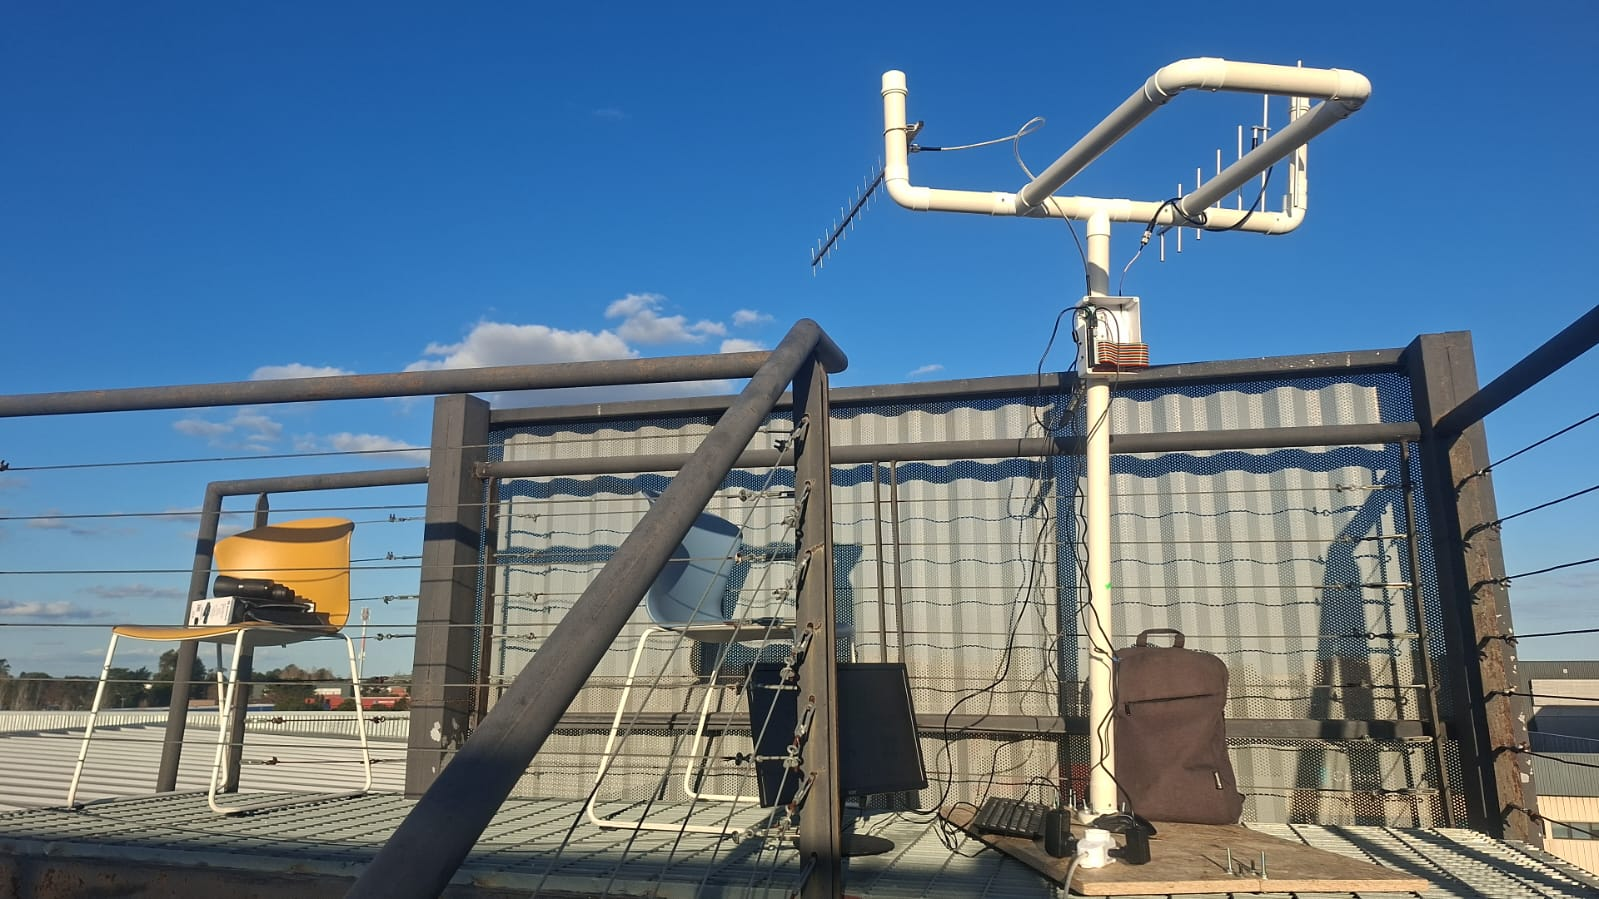
\includegraphics[width=3.3106in,keepaspectratio]{./imagenes/image97.png}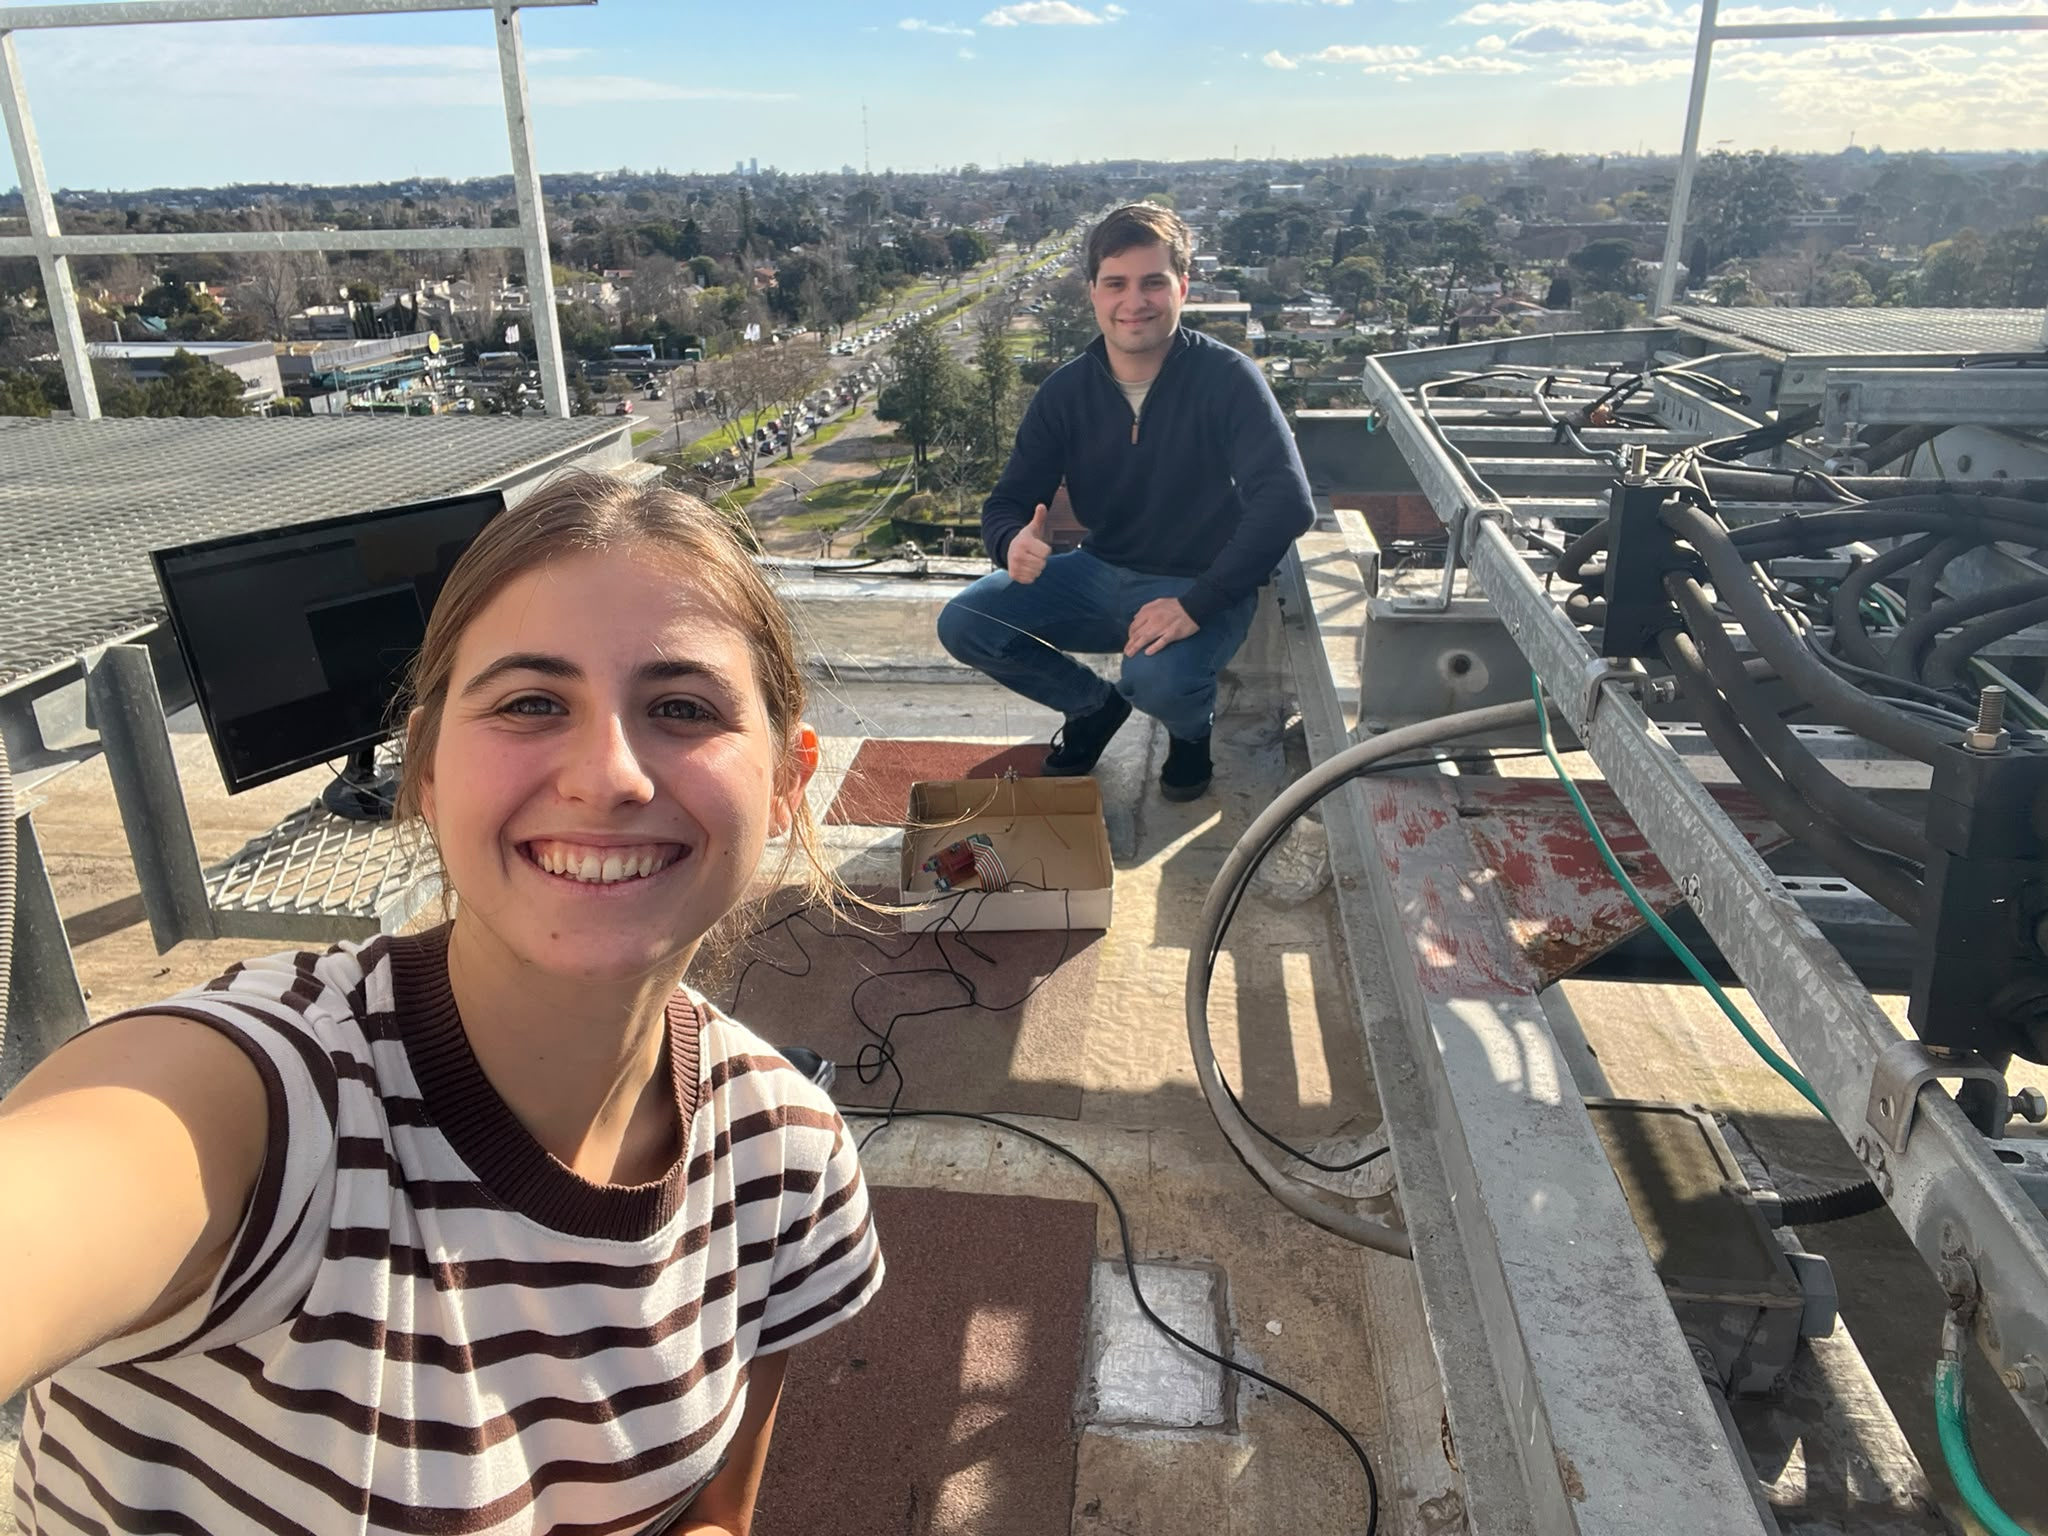
\includegraphics[width=2.4768in,keepaspectratio]{./imagenes/image52.png}

Entre el techo de un edificio y el techo de la facultad se realizó la tercera prueba de larga distancia. Se logró recibir telemetría sin atenuadores, con una pérdida de espacio libre de 93 dB. También se recibió telemetría con 50 dB de atenuación adicional. Por otro lado, se recibió vídeo sin atenuación con una pérdida de espacio libre de 103 dB. Se adiciono 10 dB de atenuación y se logró recibir video, pero después de un rato de pruebas, se dejó de recibir video con y sin atenuación. Se sospecha que se debió a una falla con un cable que se descubrió en una prueba posterior.

\subsection{Simulación con separación de 8,2 km}\label{simulaciuxf3n-larga-distancia-con-separaciuxf3n-de-8.2-km}
Se realizó una cuarta prueba de larga distancia entre la plaza Virgilio y el faro de punta carretas. Adicionalmente, el objetivo de la prueba era verificar que las antenas funcionan a largas distancias. Para el enlace de telemetría, se tenían 103,45 dB de atenuación de espacio libre a 8,2 kilómetros y se adiciono 40 dB con atenuadores.

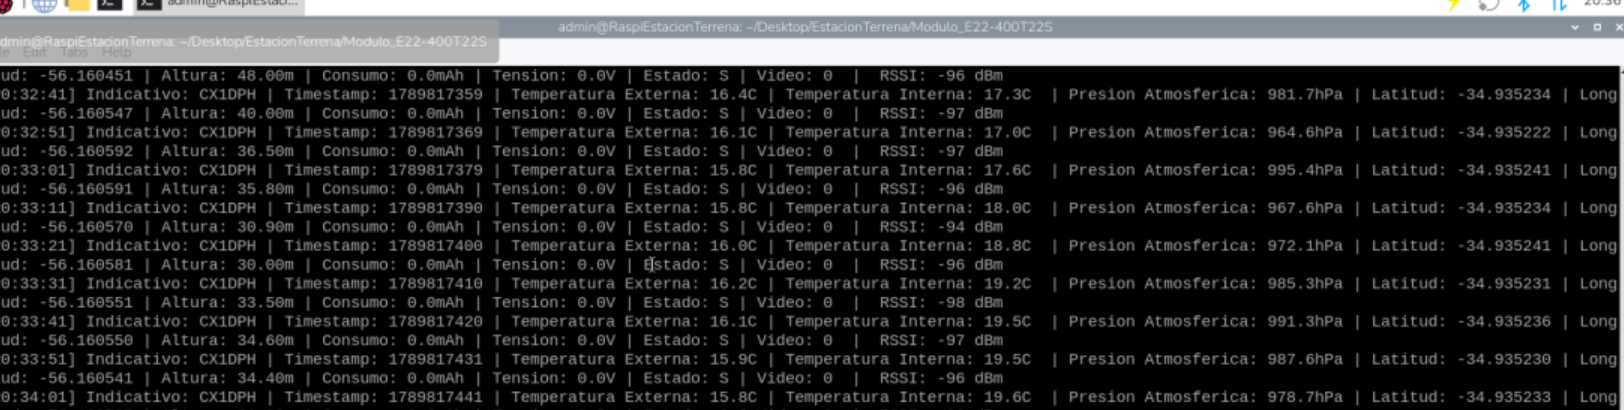
\includegraphics[width=3.7510in,keepaspectratio]{./imagenes/prueba-4-sin-atenuadores.png}

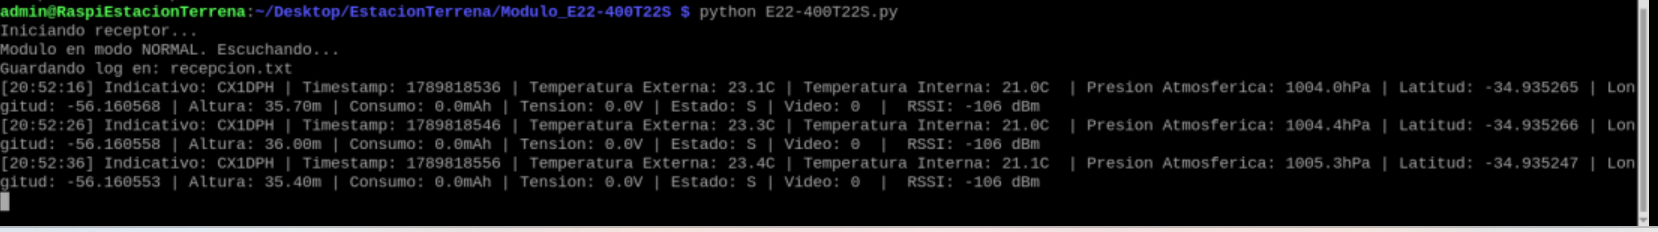
\includegraphics[width=3.7510in,keepaspectratio]{./imagenes/prueba-4-con-atenuadores.png}

Para el enlace de video, se tenían 112.58 dB de atenuación de espacio libre. Se logró recibir video, agregando 20 dB de atenuación, es decir, simulando una distancia de 82 kilómetros. Solo se tenian atenuadores de 10 y 20 dB, no se logro recibir video con mas atenuacion.

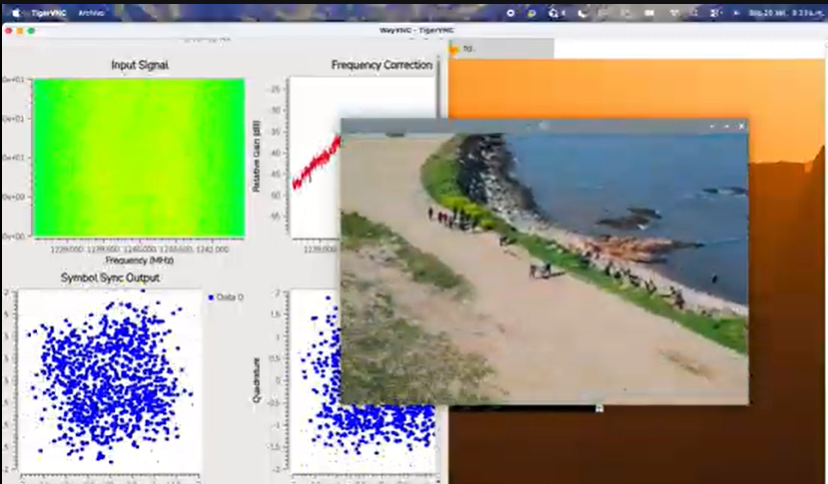
\includegraphics[width=3.7510in,keepaspectratio]{./imagenes/prueba-4-video-con-atenuadores.png}


\section{Vuelo y resultados}\label{vuelo-resultados}

\pendiente{Vuelo y resultados.}

\section{Conclusiones y trabajo futuro}\label{conclusiones}

\pendiente{Conclusiones y trabajo futuro.}

\section*{Referencias y anexos}
\phantomsection\label{referencias}
\addcontentsline{toc}{section}{\textbf{Referencias y anexos}}

\printbibliography[heading=none]

\end{document}
